\documentclass[12pt, a4paper, oneside]{report}

% --- Packages ---
\usepackage[utf8]{inputenc}
\usepackage[T1]{fontenc}
\usepackage[indonesian]{babel}
\usepackage[scaled=1.00375]{newtxtext}
\usepackage[scaled=1.00375]{newtxmath} % Word Times New Roman
\usepackage{geometry}
\usepackage[nodisplayskipstretch]{setspace}
\usepackage{titlesec}
\usepackage{enumitem}
\usepackage{fancyhdr}
\usepackage{caption}
\usepackage{subcaption}
\usepackage{tocloft}
\usepackage{indentfirst}
\usepackage{graphicx}
\graphicspath{{images/}}
\usepackage[export]{adjustbox}
\usepackage{float}
\usepackage{tikz}
\usepackage[most]{tcolorbox}
\usetikzlibrary{positioning, calc, backgrounds, fit, shapes, shapes.geometric, 
                shapes.misc, arrows.meta, decorations.pathreplacing, shadows}
\usepackage[edges]{forest}
\usepackage{everypage}
\usepackage{calc}
\usepackage{etoolbox}
\usepackage[style=english]{csquotes}
\usepackage{siunitx}
\usepackage{multirow}
\usepackage{colortbl}
\usepackage{tabularx}
\usepackage{booktabs}
\usepackage{tabularray,tblr-extras}
\usepackage{listings}
\usepackage{minted}
\usepackage{hyperref}
% \usepackage{microtype}

% Konfigurasi untuk mematikan hyphenation (pemenggalan kata)
% Agar perilaku mirip default MS Word (kata dipindah utuh ke baris baru)
\tolerance=1
\emergencystretch=\maxdimen
\hyphenpenalty=10000
\hbadness=10000
\frenchspacing

\usemintedstyle{colorful}
\setminted{
    fontsize=\scriptsize,
    breaklines=true,
    frame=none,
    bgcolor=background
}

\colorlet{punct}{red!60!black}
\definecolor{background}{HTML}{EEEEEE}
\definecolor{delim}{RGB}{20,105,176}
\colorlet{numb}{magenta!60!black}

% \lstdefinelanguage{json}{
%     basicstyle=\normalfont\ttfamily\footnotesize,
%     numbers=left,
%     numberstyle=\scriptsize,
%     stepnumber=1,
%     numbersep=8pt,
%     showstringspaces=false,
%     breaklines=true,
%     frame=lines,
%     backgroundcolor=\color{background},
%     literate=
%      *{0}{{{\color{numb}0}}}{1}
%       {1}{{{\color{numb}1}}}{1}
%       {2}{{{\color{numb}2}}}{1}
%       {3}{{{\color{numb}3}}}{1}
%       {4}{{{\color{numb}4}}}{1}
%       {5}{{{\color{numb}5}}}{1}
%       {6}{{{\color{numb}6}}}{1}
%       {7}{{{\color{numb}7}}}{1}
%       {8}{{{\color{numb}8}}}{1}
%       {9}{{{\color{numb}9}}}{1}
%       {:}{{{\color{punct}{:}}}}{1}
%       {,}{{{\color{punct}{,}}}}{1}
%       {\{}{{{\color{delim}{\{}}}}{1}
%       {\}}{{{\color{delim}{\}}}}}{1}
%       {[}{{{\color{delim}{[}}}}{1}
%       {]}{{{\color{delim}{]}}}}{1},
% }

\sisetup{
    range-phrase = {--},
    range-units = single
}

\setlength{\headheight}{52pt}

% --- Bibliography (APA 7) ---
\usepackage[
    backend=biber, 
    style=apa, 
    uniquelist=false,
    sortcites=true,
    sorting=nyt,
    date=year,
    labeldate=year,
    alldates=year,
    urldate=short,
    maxcitenames=3,
]{biblatex}
% \usepackage[
%     backend=biber, 
%     style=apa, 
% ]{biblatex}
\addbibresource{Thesis.bib}

\DeclareSourcemap{
  \maps[datatype=bibtex]{
    \map{
      \step[fieldset=addendum, null]
      \step[fieldset=note, null]
    } 
  }
}

% Custom Indonesian support for APA 7
\DeclareLanguageMapping{indonesian}{indonesia}

% --- Margins ---
\geometry{
    top=4cm,
    bottom=3cm,
    left=4cm,
    right=3cm
}

% --- Paragraph Indentation ---
\setlength{\parindent}{1cm}

% Mengatur indentasi paragraf agar menyesuaikan dengan hierarki heading
% Nilai ini mungkin perlu disesuaikan agar pas dengan panjang teks judul (x.x, x.x.x, dst)
\pretocmd{\chapter}{\setlength{\parindent}{1cm}}{}{}
\pretocmd{\section}{\setlength{\parindent}{1cm}}{}{}
\pretocmd{\subsection}{\setlength{\parindent}{1.25cm}}{}{}
\pretocmd{\subsubsection}{\setlength{\parindent}{1.5cm}}{}{}

% --- List Styling ---
% Mengatur indentasi list agar label sejajar dengan indentasi paragraf
\setlist[enumerate]{leftmargin=*, labelindent=\parindent, align=left}
\setlist[itemize]{leftmargin=*, labelindent=\parindent, align=left}

% --- Line Spacing ---
\newcommand{\wordonespacing}{0.955212}  
\newcommand{\wordonehalfspacing}{1.432818}
\setstretch{\wordonehalfspacing}

% --- Custom Commands ---
\newcommand{\imgplaceholder}[1]{%
    \fbox{%
        \begin{minipage}{0.8\textwidth}
            \centering
            \vspace{2cm}
            Gambar Placeholder:\\
            \texttt{\detokenize{#1}}
            \vspace{2cm}
        \end{minipage}%
    }%
}

\newcommand*{\myonehalfvspace}{20.775861pt}

% --- Chapter Titles ---
\titleformat{\chapter}[block]
  {\bfseries\normalsize\centering\setstretch{\wordonespacing}}
  {\MakeUppercase{\chaptername\ \Roman{chapter}}\\}
  {0pt}
  {\MakeUppercase}

\titlespacing*{\chapter}{0pt}{0pt}{\baselineskip}

% --- Float placement tuning ---
% Source - https://tex.stackexchange.com/a/77811
% Posted by Dr. Manuel Kuehner, modified by community. See post 'Timeline' for change history
% Retrieved 2026-02-24, License - CC BY-SA 4.0

\setcounter{topnumber}{2}
\setcounter{bottomnumber}{2}
\setcounter{totalnumber}{4}
\renewcommand{\topfraction}{0.85}
\renewcommand{\bottomfraction}{0.85}
\renewcommand{\textfraction}{0.15}
\renewcommand{\floatpagefraction}{0.8}
\renewcommand{\textfraction}{0.1}
% \setlength{\floatsep}{5pt plus 2pt minus 2pt}
% \setlength{\textfloatsep}{5pt plus 2pt minus 2pt}
% \setlength{\intextsep}{5pt plus 2pt minus 2pt}

% --- Section Titles ---
\setcounter{secnumdepth}{5}
\renewcommand{\thechapter}{\Roman{chapter}}
\renewcommand{\thesection}{\arabic{chapter}.\arabic{section}}
\renewcommand{\thefigure}{\arabic{chapter}.\arabic{figure}}
\renewcommand{\thetable}{\arabic{chapter}.\arabic{table}}
\renewcommand{\theequation}{\arabic{chapter}.\arabic{equation}}

\titleformat{\section}
  {\bfseries\normalsize}
  {\thesection}
  {1em}
  {}

\titlespacing*{\section}{0pt}{0pt}{0pt}

\titleformat{\subsection}
  {\bfseries\normalsize}
  {\thesubsection}
  {1em}
  {}

\titlespacing*{\subsection}{0pt}{0pt}{0pt}

\titleformat{\subsubsection}
  {\bfseries\normalsize}
  {\thesubsubsection}
  {1em}
  {}

\titlespacing*{\subsubsection}{0pt}{0pt}{0pt}

\titleformat{\paragraph}
  {\bfseries\normalsize}
  {\theparagraph}
  {1em}
  {}

\titlespacing*{\paragraph}{0pt}{0pt}{0pt}

\titleformat{\subparagraph}
  {\bfseries\normalsize}
  {\thesubparagraph}
  {1em}
  {}

\titlespacing*{\subparagraph}{0pt}{0pt}{0pt}

% --- Page Numbering ---
\fancypagestyle{frontmatter}{
    \fancyhf{}
    \fancyfoot[C]{\thepage}
    \renewcommand{\headrulewidth}{0pt}
}

\fancypagestyle{mainbody}{
    \fancyhf{}
    \fancyhead[R]{\thepage}
    \renewcommand{\headrulewidth}{0pt}
}

% Redefine plain style for chapter pages (automatically used on first page of chapters)
\fancypagestyle{plain}{
    \fancyhf{}
    \fancyfoot[C]{\thepage}
    \renewcommand{\headrulewidth}{0pt}
}

% --- Captions ---
\captionsetup[table]{font=normalsize, position=top, justification=centering, aboveskip=0pt, skip=6pt, labelsep=period, belowskip=0pt}
\captionsetup[figure]{font=normalsize, position=bottom, justification=centering, skip=6pt, labelsep=period, belowskip=-5pt}
\DefTblrTemplate{caption-sep}{default}{.\enspace}
\DefTblrTemplate{caption}{default}{%
  {\normalsize\centering
  \UseTblrTemplate{caption-tag}{default}%
  \UseTblrTemplate{caption-sep}{default}%
  \UseTblrTemplate{caption-text}{default}\par}%
}
\DefTblrTemplate{capcont}{default}{}
\DefTblrTemplate{contfoot}{default}{}
\SetTblrOuter[longtblr]{presep=10pt, postsep=10pt}

% --- Reduce spacing after and before floats ---
\setlength{\floatsep}{5pt plus 2pt minus 2pt}
\setlength{\textfloatsep}{5pt plus 2pt minus 2pt}
\setlength{\intextsep}{5pt plus 2pt minus 2pt}

% % Custom command for source in figures/tables
% \newcommand{\source}[1]{\par\vspace{2pt}\centering \footnotesize Sumber: #1 \par}

% --- Table of Contents ---
\AddEverypageHook{\addtocontents{toc}{
\protect\cftsetpnumwidth{\widthof{\thepage}-.2em}
}}
\AddEverypageHook{\addtocontents{lof}{
\protect\cftsetpnumwidth{\widthof{\thepage}-.2em}
}}
\AddEverypageHook{\addtocontents{lot}{
\protect\cftsetpnumwidth{\widthof{\thepage}-.2em}
}}
\AddEverypageHook{\addtocontents{equ}{
\protect\cftsetpnumwidth{\widthof{\thepage}-.2em}
}}
\setcounter{tocdepth}{4}
\addto\captionsindonesian{
    \renewcommand{\contentsname}{DAFTAR ISI}
    \renewcommand{\listfigurename}{DAFTAR GAMBAR}
    \renewcommand{\listtablename}{DAFTAR TABEL}
}

% Remove vertical space between chapters in LOF and LOT
\makeatletter
\patchcmd{\@chapter}{\addtocontents{lof}{\protect\addvspace{10pt}}}{}{}{}
\patchcmd{\@chapter}{\addtocontents{lot}{\protect\addvspace{10pt}}}{}{}{}
\makeatother

\renewcommand{\cftdotsep}{0.5}
\renewcommand{\cftchapleader}{\cftdotfill{\cftdotsep}} % Add dots to chapters in TOC
\renewcommand{\cftchappresnum}{BAB }
\setlength{\cftchapnumwidth}{0pt}
\renewcommand{\cfttoctitlefont}{\hfill\bfseries\normalsize}
\renewcommand{\cftaftertoctitle}{\hfill}
\setlength{\cftbeforetoctitleskip}{0pt}
\setlength{\cftaftertoctitleskip}{0pt}
\setlength{\cftbeforechapskip}{0pt}

\setlength{\cftsecindent}{0.39cm}
\setlength{\cftsubsecindent}{0.78cm}
\setlength{\cftsubsubsecindent}{1.17cm}
\setlength{\cftparaindent}{1.56cm}

\renewcommand{\cftloftitlefont}{\hfill\bfseries\normalsize}
\renewcommand{\cftafterloftitle}{\hfill}
\setlength{\cftbeforeloftitleskip}{0pt}
\setlength{\cftafterloftitleskip}{0pt}

\renewcommand{\cftlottitlefont}{\hfill\bfseries\normalsize}
\renewcommand{\cftafterlottitle}{\hfill}
\setlength{\cftbeforelottitleskip}{0pt}
\setlength{\cftafterlottitleskip}{0pt}

% Configuration for List of Figures and List of Tables entries
\renewcommand{\cftfigpresnum}{Gambar }
\renewcommand{\cfttabpresnum}{Tabel }
\setlength{\cftfigindent}{0pt}  % Align to left margin
\setlength{\cfttabindent}{0pt}  % Align to left margin
\setlength{\cftfignumwidth}{0pt} 
\setlength{\cfttabnumwidth}{0pt} 

% Use natural width for numbers (Word-like spacing)
\makeatletter
\renewcommand{\numberline}[1]{\@cftbsnum #1\@cftasnum\space}
\makeatother

% --- Daftar Lampiran Configuration ---
\newcommand{\listlampiranname}{DAFTAR LAMPIRAN}
\newlistof{lampiran}{lamp}{\listlampiranname}

\renewcommand{\cftlamptitlefont}{\hfill\bfseries\normalsize}
\renewcommand{\cftafterlamptitle}{\hfill}
\setlength{\cftbeforelamptitleskip}{0pt}
\setlength{\cftafterlamptitleskip}{0pt}

\newcommand{\buatlampiran}[1]{%
    \refstepcounter{lampiran}%
    \section*{Lampiran \thelampiran \ #1}%
    \addcontentsline{lamp}{lampiran}{Lampiran \thelampiran \ #1}%
}

% --- Daftar Persamaan Configuration ---
\newcommand{\listequationsname}{DAFTAR PERSAMAAN}
\newlistof{equations}{equ}{\listequationsname}
\newcommand{\daftarpersamaan}[1]{%
    \addcontentsline{equ}{equations}{Persamaan \theequation\quad #1}%
}

\renewcommand{\cftequtitlefont}{\hfill\bfseries\normalsize}
\renewcommand{\cftafterequtitle}{\hfill}
\setlength{\cftbeforeequtitleskip}{0pt}
\setlength{\cftafterequtitleskip}{0pt}

% --- Abstract Environment ---
%TODO: Ini bakal diganti nanti metode penelitiannya. janlup diupdate
\newenvironment{abstract-id}{
    \clearpage
    \setstretch{\wordonespacing}
    \fontsize{11pt}{13pt}\selectfont
}{
    \par
}

\newenvironment{abstract-en}{
    \clearpage
    \setstretch{\wordonespacing}
    \fontsize{11pt}{13pt}\selectfont
    \itshape
}{
    \par
}

% --- Metadata ---
\newcommand{\thesistitle}{INTEGRASI RETRIEVAL-AUGMENTED GENERATION DAN DETEKSI OBJEK MULTIMODAL PADA SISTEM AGENTIK UNTUK IDENTIFIKASI PENYAKIT TANAMAN}
\newcommand{\thesistitleen}{INTEGRATION OF RETRIEVAL-AUGMENTED GENERATION AND MULTIMODAL OBJECT DETECTION IN AN AGENTIC SYSTEM FOR PLANT DISEASE IDENTIFICATION}
\newcommand{\authorname}{Andakara Athaya Sidiq}
\newcommand{\studentid}{2200822}
\newcommand{\prody}{PROGRAM STUDI S1 TEKNIK KOMPUTER}
\newcommand{\faculty}{UNIVERSITAS PENDIDIKAN INDONESIA}
\newcommand{\campus}{KAMPUS UPI DI CIBIRU}
\newcommand{\thesisyear}{2026}

% --- Advisor and Program Head ---
\newcommand{\advisorone}{Dr. Eng. Munawir, S.Kom., M.T.}
\newcommand{\advisoronenip}{920200819851205101}
\newcommand{\advisortwo}{Muhammad Taufik Dwi Putra, S.Tr.Kom., M.T.I.}
\newcommand{\advisortwonip}{920200819940117101}
\newcommand{\programhead}{Anugrah Adiwilaga, S.ST., M.T.}
\newcommand{\programheadnip}{920200819880813101}

\begin{document}

% --- Front Matter ---
\pagestyle{frontmatter}

% Title Page
\begin{titlepage}
    \centering
    \setstretch{\wordonehalfspacing}
    \thispagestyle{empty} % No page number on title page
    {\bfseries \MakeUppercase{\thesistitle} \par}
    \vfill
    \includegraphics[width=4cm]{logo_upi.png}\par
    \vspace{\baselineskip}
    {\bfseries SKRIPSI \par}
    \vspace{\baselineskip}
    diajukan untuk memenuhi sebagian syarat untuk memperoleh gelar Sarjana Teknik Program Studi Teknik Komputer \par
    \vfill
    Oleh:\\
    \authorname\\
    \studentid
    \vfill
    {\setstretch{\wordonespacing}\bfseries \prody \\ \campus \\ \faculty \\ \thesisyear \par}
\end{titlepage}
\clearpage

\pagenumbering{roman}
\setcounter{page}{1}

% Halaman Hak Cipta
\addcontentsline{toc}{chapter}{HALAMAN HAK CIPTA}
\begin{center}
    {\bfseries HALAMAN HAK CIPTA \par}
    \vspace{0.4\baselineskip}
    {\setstretch{\wordonespacing}\bfseries \thesistitle \par}
    \vspace{3\baselineskip}
    {\setstretch{\wordonespacing} 
    Oleh\\\
    \authorname\\
    NIM \studentid
    \par}
    \vspace{2\baselineskip}
    {\setstretch{\wordonespacing}  Sebuah skripsi yang diajukan untuk memenuhi sebagian syarat memperoleh gelar Sarjana Teknik\\
    Program Studi Teknik Komputer \par}
    \vspace{\baselineskip}
    {\setstretch{\wordonespacing} \copyright\ \authorname\ \\
    Universitas Pendidikan Indonesia\\
    \thesisyear
    \par}
    \vspace{5\baselineskip}
    Hak Cipta dilindungi undang-undang.\\
    Skripsi ini tidak boleh diperbanyak seluruhnya atau sebagian,\\
    dengan dicetak ulang, difotokopi, atau cara lainnya tanpa ijin dari penulis.
\end{center}
\clearpage

% Lembar Pengajuan
\clearpage
\addcontentsline{toc}{chapter}{HALAMAN PENGESAHAN}
\begin{center}
    % \setstretch{1.1}
    {\bfseries HALAMAN PENGESAHAN SKRIPSI \par}
    \vspace{\baselineskip}
    {\bfseries \MakeUppercase{\authorname} \par}
    {\bfseries \studentid \par}
    \vspace{\baselineskip}
    {\bfseries \MakeUppercase{\thesistitle} \par}
    \vspace{\baselineskip}
    Disetujui dan Disahkan Oleh Pembimbing: \\
    Pembimbing 1 \\
    \vfill
    \advisorone \par
    NIP. \advisoronenip \\
    \vspace{\baselineskip}
    Pembimbing 2 \\
    \vfill
    \advisortwo \par
    NIP. \advisortwonip \\
    \vspace{\baselineskip}
    Mengetahui, \\
    Ketua Program Studi S-1 Teknik Komputer \\
    \vfill
    \programhead \par
    NIP. \programheadnip
\end{center}
\clearpage

% Pernyataan Bebas Plagiarisme
\clearpage
\addcontentsline{toc}{chapter}{PERNYATAAN BEBAS PLAGIARISME}
\begin{center}
    % \setstretch{1.1}
    {\bfseries PERNYATAAN BEBAS PLAGIARISME \par}
\end{center}
\vspace{\baselineskip}

\noindent Saya yang bertanda tangan di bawah ini: \par
\noindent
\begin{tabular}{@{}l p{0.2cm} l}
    Nama & : & \authorname \\
    NIM & : & \studentid \\
    Program Studi & : & Teknik Komputer \\
    Judul Karya & : & \parbox[t]{11cm}{\thesistitle}
\end{tabular}
\vspace{\baselineskip}
\begin{center}
Dengan ini menyatakan bahwa karya tulis ini merupakan hasil kerja saya sendiri. Saya menjamin bahwa seluruh isi karya ini, baik sebagian maupun keseluruhan, bukan merupakan plagiarisme dari karya orang lain, kecuali pada bagian yang telah dinyatakan dan disebutkan sumbernya dengan jelas. \par
\vspace{\baselineskip}
Jika di kemudian hari ditemukan pelanggaran terhadap etika akademik atau unsur plagiarisme, saya bersedia menerima sanksi sesuai peraturan yang berlaku di Universitas Pendidikan Indonesia.\par
\end{center}

\vfill
\begin{center}
    Bandung, 15 Januari \thesisyear \\
    \vspace{2.5cm}
    \authorname
\end{center}
\vspace{1.5cm}
\clearpage

% Kata Pengantar
\chapter*{KATA PENGANTAR}
\addcontentsline{toc}{chapter}{KATA PENGANTAR}

Puji syukur ke hadirat Allah Swt. atas segala rahmat dan karunia-Nya, sehingga penulis dapat menyelesaikan skripsi berjudul “Integrasi \textit{Retrieval-Augmented Generation} dan Deteksi Objek \textit{Multimodal} pada Sistem Agentik Untuk Identifikasi Penyakit Tanaman”. Penyusunan skripsi ini dilakukan untuk memenuhi sebagian syarat memperoleh gelar Sarjana pada Program Studi S1 Teknik Komputer, Universitas Pendidikan Indonesia.

Penulis menyadari bahwa terselesaikannya karya ini tidak terlepas dari dukungan, bimbingan, dan bantuan berbagai pihak. Oleh karena itu, pada kesempatan ini penulis menyampaikan terima kasih kepada:

\begin{enumerate}[label=\arabic*., leftmargin=*, nosep]
    \item Allah Swt. yang telah melimpahkan kesehatan, kekuatan, dan kelancaran dalam setiap tahapan penyelesaian skripsi ini.
    \item Keluarga tercinta atas doa, motivasi, serta dukungan moril dan materil yang senantiasa diberikan.
    \item Bapak Anugrah Adiwilaga, S.ST., M.T., selaku Ketua Program Studi S1 Teknik Komputer atas dukungan dan fasilitas selama masa perkuliahan.
    \item Bapak \advisorone, selaku Dosen Pembimbing I, yang telah meluangkan waktu dan pikiran untuk memberikan bimbingan, arahan, serta kesempatan yang sangat berharga bagi penulis untuk dapat menyelesaikan skripsi ini.
    \item Bapak \advisortwo, selaku Dosen Pembimbing II, yang telah memberikan banyak arahan, motivasi, serta saran-saran membangun yang membantu penulis dalam menyempurnakan skripsi ini.
    \item Bapak dan Ibu Dosen Program Studi Teknik Komputer serta seluruh civitas akademik Universitas Pendidikan Indonesia di Kampus Cibiru atas jasa dan kebaikannya selama masa perkuliahan.
    \item Rekan-rekan mahasiswa Teknik Komputer angkatan 2022 yang telah menjadi teman seperjuangan selama masa perkuliahan.
    \item Semua pihak yang tidak dapat penulis sebutkan satu per satu, yang telah memberikan bantuan baik secara langsung maupun tidak langsung dalam penyelesaian skripsi ini.
\end{enumerate}

Penulis menyadari bahwa skripsi ini masih memiliki banyak kekurangan. Oleh karena itu, kritik dan saran yang membangun sangat diharapkan demi perbaikan di masa mendatang. Semoga karya ini dapat memberikan manfaat bagi perkembangan ilmu pengetahuan dan pembaca sekalian.

\vspace{1cm}
\begin{flushright}
    Bandung, 15 Januari \thesisyear \\
    \vspace{1.5cm}
    \authorname
\end{flushright}

% Abstrak
\begin{abstract-id}
    \addcontentsline{toc}{chapter}{ABSTRAK}
    \begin{center}
        {\bfseries \MakeUppercase{\thesistitle} \par}
        \vspace{2em}
        \authorname \\
        \studentid \\
        \vspace{2em}
        {\bfseries ABSTRAK}
    \end{center}
    \vspace{-0.5em}
    Penyakit tanaman merupakan ancaman utama bagi produktivitas pertanian global. Keterbatasan metode identifikasi tradisional mendorong kebutuhan akan solusi berbasis teknologi cerdas yang cepat dan akurat. Penelitian ini bertujuan mengembangkan sistem agentik untuk identifikasi penyakit tanaman dengan mengintegrasikan deteksi \textit{multimodal} melalui \textit{Vision-Language Models} (VLM) dan kerangka kerja \textit{Retrieval-Augmented Generation} (RAG). Metode penelitian yang digunakan adalah \textit{Design and Development} (D\&D). Sistem dibangun menggunakan ekosistem LangChain dengan mengadopsi pola \textit{Reasoning and Acting} (ReAct) pada agen \textit{Large Language Models} (LLM) dari keluarga model Gemini. Komponen sistem meliputi YOLOv11 untuk deteksi daun, OWLv2 sebagai deteksi \textit{open-vocabulary}, SCOLD yang mengadopsi arsitektur CLIP untuk pengambilan gambar–teks penyakit tanaman, serta mekanisme RAG untuk pengambilan informasi dari basis pengetahuan dan internet. Hasil penelitian menunjukkan bahwa varian YOLOv11s memberikan keseimbangan terbaik dengan mAP50 sebesar \qty{89}{\percent} dan latensi median \qty{47}{ms}. Konfigurasi RAG yang menggabungkan gemini-embedding-001, BM25, dan rerank-2.5 dari Voyage AI mencapai skor NDCG@5 sebesar \qty{95.6}{\percent}, MRR@5 sebesar \qty{95.9}{\percent}, dan \textit{Recall}@5 sebesar \qty{98.0}{\percent}. Evaluasi sistem agentik pada data di dalam distribusi menunjukkan rata-rata \textit{agent goal accuracy} \qty{96}{\percent} dan \textit{disease accuracy} \qty{90}{\percent}, dengan metrik pendukung lainnya di atas \qty{90}{\percent}. Pada data di luar distribusi, sistem mencapai \textit{agent goal accuracy} \qty{81}{\percent} dan \textit{disease accuracy} \qty{70}{\percent}, dengan metrik pendukung lainnya di atas \qty{88}{\percent}. Pengujian \textit{black-box} menunjukkan seluruh fungsionalitas antarmuka sistem berjalan sesuai harapan. Integrasi ini menghasilkan sistem identifikasi penyakit tanaman yang fleksibel, adaptif, dan mampu memberikan rekomendasi penanganan yang faktual.
    
    \vspace{1em}
    \noindent {\bfseries Kata Kunci:} Identifikasi Penyakit Tanaman, Sistem Agentik, \textit{Large Language Models}, \textit{Vision-Language Models}, \textit{Retrieval-Augmented Generation}
\end{abstract-id}

\begin{abstract-en}
    \addcontentsline{toc}{chapter}{ABSTRACT}
    \begin{center}
        {\bfseries \MakeUppercase{\thesistitleen} \par}
        \vspace{2em}
        \authorname \\
        \studentid \\
        \vspace{2em}
        {\bfseries ABSTRACT}
    \end{center}
    \vspace{-0.5em}
    Plant diseases pose a major threat to global agricultural productivity. The limitations of traditional identification methods drive the need for fast and accurate intelligent technology-based solutions. This study aims to develop an agentic system for plant disease identification by integrating multimodal detection via \textit{Vision-Language Models} (VLMs) and the \textit{Retrieval-Augmented Generation} (RAG) framework. The research method employed is \textit{Design and Development} (D\&D). The system is built using the LangChain ecosystem, adopting the \textit{Reasoning and Acting} (ReAct) pattern in \textit{Large Language Model} (LLM) agents from the Gemini model family. System components include YOLOv11 for leaf detection, OWLv2 for \textit{open-vocabulary} detection, the SCOLD model—which adopts the CLIP architecture—for plant disease image-text retrieval, and a RAG mechanism for retrieving information from knowledge bases and the internet. The results indicate that the YOLOv11 \textit{small} model variant offers the best balance, with an mAP50 of \qty{89}{\percent} and a p50 latency of \qty{47}{ms}. The RAG configuration combining gemini-embedding-001, BM25, and rerank-2.5 from Voyage AI achieved NDCG@5 of \qty{95.6}{\percent}, MRR@5 of \qty{95.9}{\percent}, and \textit{Recall}@5 of \qty{98.0}{\percent}. Evaluation of the agentic system on in-distribution data showed an average \textit{agent goal accuracy} of \qty{96}{\percent} and \textit{disease accuracy} of \qty{90}{\percent}, with other supporting metrics above \qty{90}{\percent}. On out-of-distribution data, the system achieved an \textit{agent goal accuracy} of \qty{81}{\percent} and \textit{disease accuracy} of \qty{70}{\percent}, with other supporting metrics above \qty{88}{\percent}. \textit{Black-box} testing demonstrated that all system interface functionalities performed as expected. This integration results in a flexible and adaptive plant disease identification system capable of providing factual treatment recommendations.
    
    \vspace{1em}
    \noindent {\bfseries Keywords:} Plant Disease Identification, Agentic System, Large Language Models, Vision-Language Models, Retrieval-Augmented Generation.
\end{abstract-en}

\clearpage
\begingroup
\setlength{\cftaftertoctitleskip}{0pt}
\begin{singlespace}
\tableofcontents
\end{singlespace}
\clearpage

% Daftar Tabel
\addcontentsline{toc}{chapter}{\listtablename}
{%
\renewcommand{\addvspace}[1]{}%
\listoftables
}
\clearpage

% Daftar Gambar
\addcontentsline{toc}{chapter}{\listfigurename}
{%
\renewcommand{\addvspace}[1]{}%
\listoffigures
}
\clearpage

% Daftar Persamaan
\addcontentsline{toc}{chapter}{\listequationsname}
{%
\renewcommand{\addvspace}[1]{}%
\listofequations
}
\clearpage

% Daftar Lampiran
\addcontentsline{toc}{chapter}{\listlampiranname}
{%
\renewcommand{\addvspace}[1]{}%
\listoflampiran
}
\clearpage



\clearpage

\endgroup
\clearpage

% --- Main Body ---
\pagenumbering{arabic}
\pagestyle{mainbody}

\chapter{PENDAHULUAN}

\section{Latar Belakang Penelitian}
Penyakit merupakan salah satu faktor utama yang memengaruhi produktivitas dan kualitas tanaman. Secara garis besar, penyakit tanaman dapat diklasifikasikan menjadi dua kategori, yakni penyakit abiotik dan penyakit biotik \parencite{bhargavaPlantLeafDisease2024}. Penyakit abiotik disebabkan oleh faktor lingkungan non-hidup, seperti kondisi tanah, suhu, atau kelembaban yang tidak ideal, yang dapat melemahkan tanaman dan membuatnya lebih rentan. Sementara itu, penyakit biotik disebabkan oleh organisme hidup penyebab penyakit (patogen), seperti jamur, bakteri, atau virus. Penyakit abiotik umumnya lebih responsif terhadap perbaikan kondisi lingkungan seperti penyesuaian penyiraman dan pemberian nutrisi, sedangkan penyakit biotik lebih sulit ditangani karena membutuhkan identifikasi yang akurat terhadap patogen penyebabnya \parencite{bhargavaPlantLeafDisease2024}. 

\textcite{fao2020climate} melaporkan penyakit tanaman menjadi salah satu ancaman utama kerugian hasil panen, di mana sekitar \qtyrange{20}{40}{\percent} hasil panen global hilang setiap tahunnya akibat serangan hama dan penyakit tanaman. \textcite{gullinoPositioningPlantHealth2024} menyebutkan bahwa tekanan lingkungan, khususnya perubahan iklim, semakin memperparah ancaman ini. Hal ini karena pemanasan global dan perubahan pola cuaca mengubah siklus hidup patogen serta sebaran geografisnya, menyebarkan penyakit ke wilayah-wilayah baru, dan memperbesar risiko wabah penyakit. Kondisi ini menunjukkan bahwa penyakit tanaman merupakan ancaman serius bagi produktivitas pertanian, yang menuntut perhatian dan upaya pengendalian. Upaya pengendalian ini diawali dengan identifikasi yang tepat terhadap gejala yang muncul pada tanaman.

Patogen penyebab penyakit tanaman biasanya menyerang daun terlebih dahulu sebelum menginfeksi seluruh tanaman \parencite{sharmaClassificationPlantLeaf2020}. Gejala penyakit tanaman yang paling mudah dikenali oleh mata manusia umumnya berupa bercak pada daun, meskipun ada penyakit yang tidak menampakkan gejala pada daun sama sekali dan ada pula yang baru terlihat pada tahap lanjut setelah tanaman mengalami kerusakan signifikan \parencite{upadhyayDeepLearningComputer2025}. Dalam praktik tradisional berarti identifikasi penyakit dilakukan dengan mengamati gejala tersebut secara visual oleh petani atau ahli yang memakan waktu dan bergantung pada ketersediaan tenaga ahli \parencite{bhargavaPlantLeafDisease2024}. Teknik laboratorium dapat memastikan identifikasi patogen penyebab penyakit secara spesifik, namun membutuhkan biaya yang relatif mahal dan memerlukan peralatan khusus serta keahlian tinggi \parencite[Sahu dkk., 2021 dalam ][]{upadhyayDeepLearningComputer2025}. Keterbatasan metode identifikasi tradisional dan laboratorium mendorong kebutuhan akan pendekatan baru yang lebih cepat, akurat, dan dapat diakses secara luas dalam mendeteksi penyakit tanaman.

Terobosan dalam \textit{artificial intelligence} (AI) kini mendorong identifikasi penyakit tanaman melalui pendekatan \textit{deep learning} dan \textit{computer vision} \parencite{upadhyayDeepLearningComputer2025}. \textit{Computer vision} adalah bidang AI yang memungkinkan komputer memahami informasi dari data visual seperti gambar atau video. Dalam identifikasi penyakit tanaman, teknologi ini dimanfaatkan untuk mengenali gejala visual melalui ciri seperti perubahan warna, bentuk area gejala, dan tekstur guna membedakan tanaman sehat dan terinfeksi. Seiring perkembangannya, \textit{computer vision} sering dikombinasikan dengan \textit{deep learning} \parencite{bhargavaPlantLeafDisease2024, upadhyayDeepLearningComputer2025}. Daun merupakan bagian tanaman yang paling memperlihatkan gejala penyakit, sehingga sebagian besar penelitian memanfaatkan gambar daun sebagai data pelatihan. Model \textit{deep learning} dilatih untuk mengenali pola visual, termasuk variasi warna, bentuk, dan tekstur daun yang menjadi indikator penyakit \parencite{ramanjotPlantDiseaseDetection2023}. Pendekatan ini memungkinkan deteksi penyakit secara otomatis tanpa ketergantungan penuh pada tenaga ahli maupun prosedur laboratorium yang kompleks.

\textcite{upadhyayDeepLearningComputer2025} memaparkan berbagai teknik \textit{deep learning} telah diterapkan untuk identifikasi penyakit tanaman. Teknik-teknik ini meliputi \textit{image recognition} (pengenalan citra) untuk klasifikasi jenis penyakit, \textit{object detection} (deteksi objek) untuk mendeteksi keberadaan penyakit, hingga \textit{vision-language models} (VLMs) yang mengintegrasikan pemrosesan informasi visual dan tekstual. Arsitektur VLM umumnya terdiri dari dua komponen utama, yaitu \textit{vision encoder} untuk mengekstraksi fitur dari data citra dan \textit{language model} untuk memproses informasi tekstual serta fitur visual yang telah diekstraksi \parencite{bordesIntroductionVisionLanguageModeling2024}. VLM sering dibangun di atas kemampuan \textit{large language models} (LLMs) \parencite{bordesIntroductionVisionLanguageModeling2024, quocVisionLanguageFoundationModel2025}, yaitu model AI yang dilatih pada data teks dalam skala masif untuk memahami, meringkas, dan menghasilkan bahasa. Sinergi ini memungkinkan sistem memproses data multimodal, yaitu data yang menggabungkan berbagai modalitas informasi seperti citra dan teks secara bersamaan. Identifikasi penyakit tidak hanya terbatas pada label klasifikasi visual, tetapi juga dapat disertai konteks deskriptif yang komprehensif.

Penerapan teknologi ini didorong oleh paradigma \textit{foundation models}, yaitu model yang dilatih pada skala data sangat masif dan beragam agar dapat diadaptasi untuk berbagai tugas hilir (\textit{downstream tasks}) \parencite{bommasaniOpportunitiesRisksFoundation2022}. Model-model ini, seperti GPT-3 dari \textcite{brownLanguageModelsAre2020} untuk pemrosesan teks atau CLIP dari \textcite{radfordLearningTransferableVisual2021} untuk tugas \textit{vision-language}, dirancang sebagai dasar yang dapat disesuaikan untuk berbagai aplikasi spesifik \parencite{radfordLearningTransferableVisual2021, liuSwinTransformerHierarchical2021}. Berkat kemunculan \textit{foundation models}, LLM telah diadopsi secara luas di berbagai domain. Kini prinsip tersebut dapat diperluas melalui VLM untuk menangani tantangan identifikasi penyakit tanaman sebagai perkembangan dari metode sebelumnya.

Tantangan utama pada identifikasi penyakit tanaman apabila melalui \textit{image recognition} terletak pada keterbatasan model konvensional. Model berbasis \textit{convolutional neural network} (CNN) masih lazim digunakan berkat kemampuannya mengekstraksi fitur secara efektif \parencite{gulmezComprehensiveReviewConvolutional2025}. Akan tetapi, CNN umumnya dilatih melalui \textit{supervised learning} untuk memetakan gambar ke kelas-kelas penyakit yang telah ditentukan sebelumnya \parencite{pacalSystematicReviewDeep2024}. Pendekatan ini menghasilkan klasifikasi yang kaku karena terbatas pada label yang tersedia selama pelatihan. Selain itu, model CNN memerlukan data latih dalam jumlah besar agar mampu mencapai performa tinggi \parencite{liuCrossModalDataFusion2025}. Pengumpulan citra penyakit tanaman dari berbagai jenis dengan kualitas yang memadai sulit dilakukan serta membutuhkan biaya dan waktu yang signifikan. Ketika jenis penyakit baru perlu ditambahkan, model harus dilatih ulang dengan data tambahan, yang berimplikasi pada kebutuhan komputasi tinggi.

Di lain sisi, pada \textit{object detection}, penelitian sebelumnya memperlihatkan bahwa YOLO (\textit{You Only Look Once}) masih mendominasi sebagai arsitektur utama untuk deteksi penyakit tanaman \parencite{ranaDetectionPlantDiseases2025}. Model ini mengadopsi pendekatan regresi tunggal yang memprediksi \textit{bounding box} dan probabilitas kelas secara langsung dari seluruh citra dalam satu langkah, sehingga sangat efisien untuk aplikasi \textit{real-time} \parencite[Redmon dkk., 2016 dalam][]{ranaDetectionPlantDiseases2025}. Dalam konteks identifikasi penyakit tanaman, YOLO telah mengalami perkembangan signifikan. YOLOv11 sebagai versi terbaru menawarkan peningkatan akurasi dan kecepatan inferensi dibandingkan pendahulunya \parencite{ranaDetectionPlantDiseases2025}. Analisis komprehensif \textcite{ramosComprehensiveAnalysisYOLO2025} membandingkan berbagai arsitektur YOLO, termasuk YOLOv8, YOLOv9, YOLOv10, YOLOv11, dan YOLOv12, untuk identifikasi penyakit daun tomat. Hasil analisis menunjukkan YOLOv11 memiliki performa paling efektif, dengan varian YOLOv11x mencapai mAP@50 sebesar 93,6\% dan mAP@50:95 sebesar 79,0\%. Dalam aplikasinya, YOLO umum diimplementasikan dalam skema \textit{two-stage detection} untuk penyakit tanaman \parencite{abhiramNovelTwoStageDeep2024a, yaoTwoStageDetectionAlgorithm2024}. Tahap pertama mendeteksi lokasi gejala pada daun dan tahap kedua mengklasifikasikan jenis penyakitnya. Pendekatan ini memungkinkan deteksi yang lebih presisi dengan kecepatan tinggi. Meskipun unggul dalam kecepatan, YOLO masih menghadapi tantangan serupa dengan CNN konvensional, yaitu ketergantungan pada data latih berlabel dalam jumlah besar dan kesulitan dalam mendeteksi penyakit yang tidak termasuk dalam kelas pelatihan \parencite{pacalSystematicReviewDeep2024}.

Pendekatan VLMs muncul sebagai solusi alternatif yang menjanjikan untuk mengatasi keterbatasan metode konvensional. Pada \textit{image recognition}, \textcite{radfordLearningTransferableVisual2021} mengembangkan CLIP (\textit{Contrastive Language-Image Pre-training}) yang memperkenalkan kemampuan \textit{zero-shot learning} dengan menggabungkan representasi visual dan teks melalui \textit{pre-training} pada skala data masif. \textit{Zero-shot learning} merupakan kemampuan model untuk mengenali kelas baru tanpa melihat contoh dari kelas tersebut selama pelatihan. Melalui \textit{zero-shot learning}, CLIP dapat mengklasifikasikan gambar tanpa memerlukan \textit{fine-tuning} pada kelas tertentu. Dalam domain penyakit tanaman, \textcite{quocVisionLanguageFoundationModel2025} mengembangkan SCOLD (\textit{Soft-target COntrastive learning for Leaf Disease identification}), model \textit{foundation vision-language} yang terinspirasi arsitektur CLIP. SCOLD dikembangkan bersama dataset LeafNet berisi pasangan gambar-teks yang secara khusus dirancang untuk identifikasi penyakit tanaman secara multimodal. Selain itu, \textcite{weiBenchmarkingInthewildMultimodal2024} juga mengembangkan dataset PlantWild berisi pasangan gambar-teks dan \textit{baseline} adopsi model CLIP untuk identifikasi penyakit tanaman. Dari dataset PlantWild, \textcite{weiSnapDiagnoseAdvanced2024} mengembangkan Snap and Diagnose untuk membangun sistem \textit{image retrieval} yang mendukung \textit{input} gambar dan teks, sehingga memungkinkan identifikasi penyakit melalui pencarian gambar serupa secara multimodal.

Selain itu pada \textit{object detection}, \textcite{pengLeafDiseaseImage2022} menunjukkan kombinasi YOLO untuk deteksi objek daun dengan \textit{deep metric learning} untuk \textit{image retrieval} mencapai akurasi 97,84\% pada \textit{closed-set identification} dan 89,09\% pada \textit{open-set identification}. Peng dkk. menekankan bahwa pendekatan ini dapat menggabungkan keunggulan YOLO dalam deteksi \textit{real-time} dengan kemampuan \textit{image retrieval} untuk mengatasi tantangan penambahan kelas baru. Sistem hanya perlu menambahkan gambar baru ke \textit{database retrieval} tanpa melatih ulang model, berbeda dengan metode klasifikasi konvensional yang memerlukan pelatihan ulang.

Pada perkembangan terbaru, transformasi signifikan terjadi dengan munculnya model \textit{vision-language} untuk \textit{object detection}. \textcite{liuGroundingDINOMarrying2025} mengembangkan Grounding DINO dengan menggabungkan detektor DINO berbasis Transformer dengan \textit{pre-training} yang memungkinkan deteksi berbasis \textit{prompt} teks bahasa natural. Grounding DINO membuka kemampuan \textit{open-vocabulary detection}, yakni deteksi objek berdasarkan deskripsi teks fleksibel tanpa batas kelas yang ditentukan sebelumnya. Hal ini memungkinkan deteksi objek baru tanpa data latih tambahan. Penelitian \textcite{singhFarmerChatScalingAIPowered2024} dan \textcite{weiBenchmarkingInthewildMultimodal2024} menunjukkan adaptasi Grounding DINO untuk deteksi tanaman dapat mencapai performa unggul bahkan dengan data terbatas. Selain Grounding DINO, \textcite{mindererScalingOpenVocabularyObject2024} memperkenalkan OWLv2 sebagai perkembangan dari OWL-ViT dengan teknik \textit{self-training} OWL-ST. OWLv2 menunjukkan performa superior dalam \textit{open-vocabulary detection}, di mana varian G/14 mencapai 47,2\% AP pada kelas \textit{rare} dataset LVIS, melampaui model sebelumnya secara signifikan. Lebih lanjut, evaluasi oleh \textcite{wuEvaluatingPerformanceOpenVocabulary2026} menunjukkan bahwa OWLv2 memiliki robustitas yang lebih baik dibandingkan Grounding DINO dan Detic dalam menghadapi degradasi kualitas citra, namun penggunaannya untuk deteksi penyakit tanaman masih belum banyak dieksplorasi.

Setelah berbagai pendekatan berbasis VLM dikembangkan, perkembangan terbaru menunjukkan upaya integrasi model deteksi objek berbasis \textit{deep learning} dengan LLM untuk identifikasi penyakit tanaman. Pada implementasi paling sederhana, \textcite{sbDesignImplementationAIPowered2024} mengembangkan sistem untuk deteksi penyakit tanaman sekaligus memberikan rekomendasi penanganan. Sistem ini memanfaatkan YOLOv5 untuk mengidentifikasi penyakit dan diintegrasikan dengan LLM dari Gemini API yang digunakan secara langsung untuk menghasilkan respons percakapan tentang penyakit tanaman. Akan tetapi, LLM digunakan secara langsung tanpa adanya augmentasi tambahan yang dapat membawa keterbatasan. \textcite{minaeeLargeLanguageModels2025} menekankan bahwa adopsi LLM pada domain tertentu memerlukan augmentasi agar dapat menghindari risiko halusinasi dan keluaran yang tidak konsisten. Salah satu pendekatan yang paling fleksibel untuk menghindari masalah ini adalah dengan memberikan sistem akses \textit{retrieval} (pencarian) ke data eksternal.

Oleh karena itu, pendekatan integratif ini selanjutnya dikembangkan oleh \textcite{mondalVisionMeetsLanguage2025} dengan menggabungkan deteksi objek dari YOLOv8 untuk identifikasi penyakit tanaman kopi secara cepat serta LLM yang diberi akses pengambilan ke \textit{knowledge base} (basis pengetahuan) tentang penyakit tanaman kopi. Akses tersebut diimplementasikan melalui kerangka \textit{retrieval-augmented generation} (RAG) sehingga respon LLM dilandasi dokumen rujukan yang relevan dan mampu menyajikan rekomendasi penanganan. Kendati demikian, pendekatan tersebut masih menyisakan keterbatasan berupa alur dari deteksi YOLOv8 ke bagian pengambilan dan generasi jawaban ditetapkan secara tetap, sehingga perilaku sistem relatif kaku dan kurang adaptif.

Menurut \textcite{anthropicBuildingEffectiveAgents2024}, sistem yang memanfaatkan LLM dengan pengambilan atau kapabilitas tambahan lain yang alurnya sudah ditentukan sejak awal dapat dikategorikan sebagai \textit{agentic system} (sistem agentik) berbasis \textit{workflow} (alur kerja). Kapabilitas tambahan tersebut disebut sebagai \textit{external tools} (alat eksternal) yang diintegrasikan untuk membantu LLM menyelesaikan tugas tertentu. Alternatif yang lebih adaptif dibandingkan \textit{workflow} adalah LLM \textit{agent} (agen), yakni sistem yang memungkinkan LLM memilih dan menggunakan alat secara fleksibel sesuai konteks tugas. Salah satu implementasi ini adalah pola \textit{reasoning and acting} (ReAct) yang diperkenalkan oleh \textcite{yaoReActSynergizingReasoning2023}. Agen LLM yang diimplementasikan dengan pola ReAct memungkinkan LLM melakukan penalaran terlebih dahulu (\textit{reasoning}) sebelum memutuskan tindakan (\textit{acting}) dengan memanggil dan menggunakan alat eksternal. ReAct telah menjadi salah satu bentuk implementasi agen paling populer \parencite{yuSurveyAgentWorkflow2025}, seiring dengan munculnya LLM modern yang mendukung penggunaan alat eksternal, seperti keluarga Gemini 2.5 \parencite{comaniciGemini25Pushing2025} dan Gemini 3 \parencite{google2025}. Dengan demikian, sistem agentik yang mengadopsi pola ReAct dapat menjadi solusi untuk mengembangkan sistem yang lebih adaptif dan fleksibel.

Akan tetapi, peningkatan fleksibilitas pada sistem agentik ini turut membawa kompleksitas baru dalam proses validasi. Evaluasi kinerja sistem agentik berbasis LLM menghadirkan tantangan tersendiri karena luarannya berupa bahasa alami yang kompleks, cair, dan tidak terstruktur \parencite{liuGEvalNLGEvaluation2023}. Metrik evaluasi heuristik BLEU (\textit{Bilingual Evaluation Understudy}) dan ROUGE (\textit{Recall-Oriented Understudy for Gisting Evaluation}) kurang bisa menangkap nuansa semantik dan koherensi dari jawaban yang dihasilkan \parencite{saiSurveyEvaluationMetrics2022}. Penilaian oleh manusia sejatinya merupakan standar emas untuk menangkap nuansa tersebut, namun proses ini cenderung lambat, mahal, dan sulit dilakukan dalam skala besar. Oleh karena itu, pendekatan \textit{LLM-as-a-judge} diperkenalkan sebagai solusi alternatif untuk memanfaatkan kemampuan LLM yang kuat dalam menilai kualitas luaran model lain menyerupai penilaian manusia \parencite{liGenerationJudgmentOpportunities2025}. Akan tetapi, penggunaan LLM sebagai evaluator juga tidak luput dari kelemahan, seperti adanya bias posisi (\textit{positional bias}) di mana model cenderung memfavoritkan jawaban yang muncul pada urutan pertama \parencite{wangLargeLanguageModels2024}. Untuk mengatasi keterbatasan tersebut dan meningkatkan akurasi evaluasi, berbagai kerangka kerja (\textit{framework}) telah dikembangkan. \textcite{liuGEvalNLGEvaluation2023} memperkenalkan G-Eval yang memanfaatkan teknik \textit{chain-of-thought} (CoT) untuk penilaian yang lebih selaras dengan preferensi manusia. Selain itu, \textit{framework} seperti RAGAS \parencite{esRagasAutomatedEvaluation2025} dan DeepEval \parencite{ipDeepeval2026} kini tersedia untuk mengevaluasi komponen sistem agentik dengan lebih andal dan terukur.

Berdasarkan tantangan dan peluang yang telah diuraikan, penelitian ini mengusulkan pengembangan sistem agentik untuk identifikasi penyakit tanaman. Sistem ini akan mengintegrasikan VLM sebagai alat pada sistem untuk mengatasi keterbatasan pendekatan konvensional. Secara spesifik, penelitian ini akan mengadopsi model \textit{foundation} seperti SCOLD untuk identifikasi penyakit berbasis \textit{image-text retrieval} atau pencarian gambar dan teks, serta mengombinasikan YOLO dengan OWLv2 untuk membantu deteksi objek tanaman dalam identifikasi penyakit. Lebih lanjut, mekanisme \textit{retrieval-augmented generation} (RAG) akan dimanfaatkan untuk memberikan akses ke basis pengetahuan yang relevan. Keseluruhan kapabilitas ini akan diintegrasikan ke dalam sebuah agen LLM yang dirancang dengan pola \textit{reasoning and acting} (ReAct), memungkinkannya untuk memilih dan menggunakan alat secara adaptif dalam proses identifikasi hingga pemberian rekomendasi penanganan. Selain itu, sistem ini akan dilengkapi dengan antarmuka berbasis web untuk memfasilitasi interaksi pengguna. Untuk mengevaluasi performa sistem agentik yang dikembangkan, penelitian ini akan menggunakan pendekatan \textit{LLM-as-a-judge} dengan kriteria evaluasi yang relevan. Melalui integrasi ini, penelitian ini diharapkan dapat menghasilkan sistem identifikasi penyakit tanaman yang tidak hanya akurat dan komprehensif, tetapi juga fleksibel dan adaptif dalam menangani berbagai kasus identifikasi penyakit tanaman.

\section{Rumusan Masalah Penelitian}
Berdasarkan uraian latar belakang, maka permasalahan yang akan dibahas dalam penelitian ini dapat dirumuskan sebagai berikut: 
\begin{enumerate}[nosep]
    \item Bagaimana pengembangan sistem agentik yang mengintegrasikan deteksi multimodal, mekanisme \textit{Retrieval-Augmented Generation} (RAG), dan pola \textit{Reasoning and Acting} (ReAct) untuk identifikasi penyakit tanaman?
    \item Bagaimana perancangan dan pengembangan antarmuka pengguna berbasis web dilakukan untuk memfasilitasi interaksi dengan sistem agentik?
    \item Bagaimana evaluasi performa sistem agentik dilakukan melalui pendekatan \textit{LLM-as-a-judge}?
\end{enumerate}

\section{Tujuan Penelitian}
Tujuan dari penelitian ini adalah: 
\begin{enumerate}[nosep]
    \item Mengembangkan sistem agentik yang mengintegrasikan deteksi multimodal, mekanisme RAG, dan pola ReAct untuk identifikasi penyakit tanaman.
    \item Merancang dan mengembangkan antarmuka pengguna berbasis web untuk memfasilitasi interaksi dengan sistem agentik.
    \item Mengevaluasi performa sistem agentik yang dikembangkan dengan pendekatan \textit{LLM-as-a-judge}.
\end{enumerate}

\section{Ruang Lingkup Penelitian}
Ruang lingkup yang menjadi batasan penelitian ini adalah: 
\begin{enumerate}[nosep]
    \item Karakteristik penyakit tanaman yang diidentifikasi oleh sistem mengikuti cakupan dan variasi gejala yang tersedia dalam dataset penyakit tanaman yang digunakan sebagai rujukan penelitian.
    \item Sistem yang dikembangkan tidak sepenuhnya mendukung bahasa Indonesia karena beberapa proses internal dan keluarannya dioptimalkan untuk bahasa Inggris menyesuaikan dataset yang digunakan. Akan tetapi, keluaran akhir sistem tetap dapat disajikan dalam bahasa Indonesia.
    \item Evaluasi sistem dibatasi pada metode \textit{offline evaluation} menggunakan dataset terkurasi untuk \textit{benchmarking} dan deteksi regresi, sedangkan evaluasi \textit{online} melalui interaksi pengguna secara \textit{real-time} belum dilakukan.
    \item Evaluasi lapangan secara langsung dengan data \textit{real-time} atau validasi jangka panjang pada praktik pertanian belum dilakukan.
    \item Luaran penelitian berupa sistem prototipe sebagai bukti konsep (\textit{proof of concept}) dan bukan merupakan aplikasi yang siap untuk komersialisasi.
\end{enumerate}

\section{Manfaat Penelitian} 
Penelitian ini diharapkan dapat memberikan kontribusi, baik dari segi pengembangan ilmu pengetahuan maupun penerapan praktis di lapangan.

\subsection{Manfaat Teoritis}
Penelitian ini berkontribusi pada pengembangan ilmu pengetahuan terkait integrasi model deteksi objek multimodal dan sistem agentik. Kajian ini memperkaya literatur mengenai penerapan pola ReAct serta RAG di bidang pertanian. Selain itu, metodologi \textit{LLM-as-a-judge} yang diterapkan dapat menjadi referensi validasi sistem agentik dengan luaran bahasa alami.

\subsection{Manfaat Praktis}
Selain manfaat teoritis, penelitian ini diharapkan memberikan manfaat praktis, antara lain:
\begin{enumerate}[nosep]
    \item Bagi petani, sistem yang dikembangkan diharapkan dapat dimanfaatkan sebagai asisten cerdas untuk mendeteksi penyakit tanaman secara dini dan akurat. Informasi diagnosis serta rekomendasi penanganan yang diberikan berpotensi membantu pengambilan keputusan yang lebih cepat tanpa ketergantungan penuh pada tenaga ahli.
    \item Bagi masyarakat umum, teknologi ini diharapkan dapat digunakan untuk memperoleh wawasan mengenai kondisi kesehatan tanaman. Hal ini berpotensi mendukung kemandirian masyarakat dalam merawat tanaman di lingkungan sekitar serta meningkatkan kesadaran akan pentingnya pengendalian penyakit tanaman.
    \item Bagi peneliti dan pengembang sistem, arsitektur sistem agentik yang diusulkan dapat menjadi rujukan bagi pengembangan solusi teknologi serupa di masa depan. Pendekatan integrasi berbagai model kecerdasan buatan serta kerangka evaluasi yang diterapkan dapat diadopsi dan disempurnakan untuk berbagai kasus penggunaan lain.
\end{enumerate}




%TODO: semua yg ada di judul wajib ada subbabnya di bab 2. termasiuk multimodal dan deteksi objek

\chapter{TINJAUAN PUSTAKA}
\section{Penyakit Tanaman}
Penyakit tanaman secara fundamental didefinisikan sebagai gangguan atau penyimpangan dari kondisi fisiologis normal yang disebabkan oleh interaksi berkelanjutan dengan faktor eksternal, yang bermanifestasi pada perubahan morfologi, fisiologi, maupun perilaku tanaman \parencite{vishnoiPlantDiseaseDetection2021}. \textcite{muhammadComprehensiveReviewCrop2025} memperluas definisi ini dengan terminologi cekaman (\textit{crop stress}), yakni segala kondisi eksternal yang memberikan dampak negatif terhadap metabolisme, pertumbuhan, dan produktivitas tanaman. Segala bentuk gangguan yang memengaruhi vitalitas tanaman tersebut menuntut adanya pemahaman ilmiah yang komprehensif.

Disiplin ilmu yang mempelajari fenomena ini adalah Fitopatologi (\textit{Phytopathology}). Berdasarkan etimologinya, istilah ini berasal dari bahasa Yunani \textit{phyton} (tanaman), \textit{pathos} (penyakit), dan \textit{logos} (pengetahuan) \parencite{bhargavaPlantLeafDisease2024}. Bhargava dkk. menjelaskan bahwa Fitopatologi bukan sekadar ilmu pengenalan penyakit, melainkan sebuah sistem terpadu yang mencakup empat tujuan utama, yaitu etiologi yang berfokus pada studi sumber atau penyebab penyakit, patogenesis yang mempelajari mekanisme perkembangan penyakit, epidemiologi yang mengkaji interaksi antara populasi inang, patogen, dan lingkungan, serta manajemen yang merancang strategi pengendalian untuk memitigasi kerugian. Fitopatologi mengintegrasikan berbagai subdisiplin ilmu seperti bakteriologi, virologi, mikologi, hingga biologi molekuler dan meteorologi untuk memahami dinamika kesehatan tanaman secara holistik.

Identifikasi penyebab cekaman pada tanaman secara mendasar dimulai dengan mengklasifikasikannya ke dalam dua kategori utama, yaitu faktor abiotik dan faktor biotik \parencite{bhargavaPlantLeafDisease2024, muhammadComprehensiveReviewCrop2025, georgePresentFutureDeep2025}. Visualisasi klasifikasi cekaman ini disajikan pada Gambar \ref{fig:taxonomy_plant_disease}. Cekaman abiotik dipicu oleh faktor lingkungan non-hidup seperti suhu ekstrem, salinitas tanah, dan ketidakseimbangan nutrisi yang bertindak sebagai stresor fisik pengganggu homeostasis tanaman \parencite{muhammadComprehensiveReviewCrop2025}. Secara karakteristik, cekaman abiotik bersifat tidak menular dengan sebaran di lahan yang cenderung seragam mengikuti kondisi fisik lingkungan, serta gejala yang muncul secara serentak pada banyak individu. Diagnosis untuk kategori ini umumnya dilakukan melalui analisis tanah, cuaca, dan jaringan tanaman. Sebaliknya, cekaman biotik disebabkan oleh organisme hidup parasit seperti jamur (\textit{fungi}), bakteri, virus, dan nematoda, maupun serangan hama yang dapat berperan sebagai vektor pembawa penyakit. Berbeda dengan faktor abiotik, cekaman biotik memiliki sifat menular yang menyebar secara bertahap seiring siklus hidup patogen, dengan pola sebaran di lahan yang cenderung berkelompok (\textit{patchy}) atau menyebar secara radial. Identifikasi cekaman biotik memerlukan pengamatan visual terhadap tanda, kultur, atau teknik molekuler.
\begin{figure}[ht]
\centering
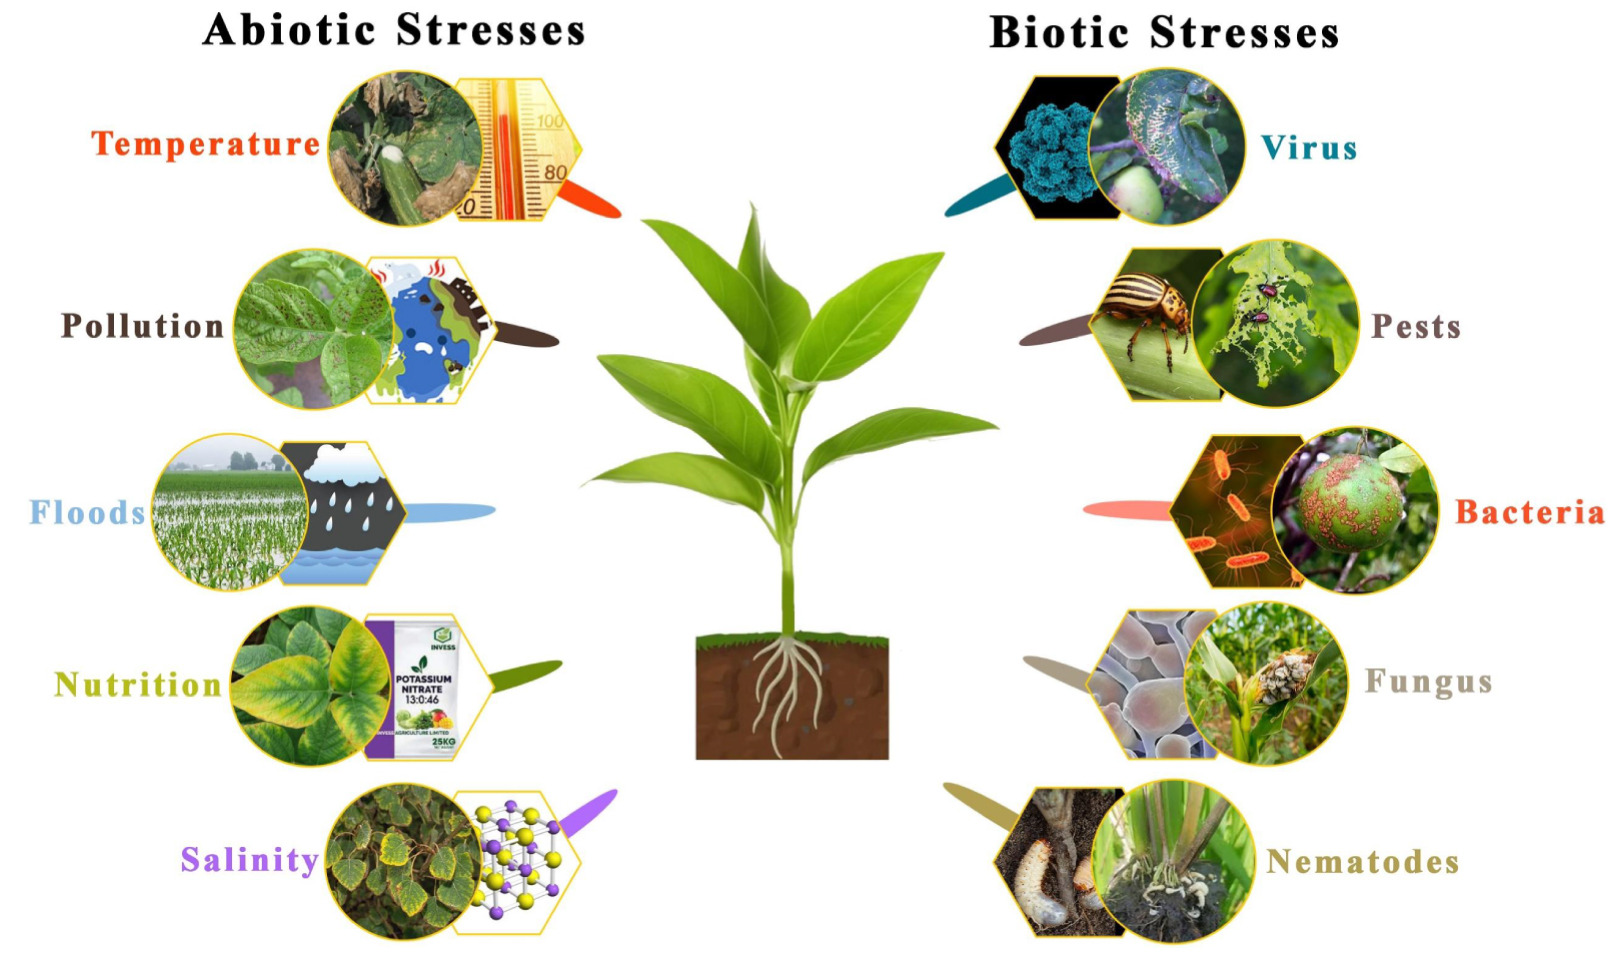
\includegraphics[width=\textwidth]{bab2/abioticvsbiotic.jpg}
\caption[Klasifikasi cekaman biotik dan abiotik pada tanaman]{Klasifikasi cekaman biotik dan abiotik pada tanaman \parencite{georgePresentFutureDeep2025}}
\label{fig:taxonomy_plant_disease}
\end{figure}

% Terjadinya penyakit biotik yang sukses memerlukan interaksi kompleks yang dikenal sebagai Segitiga Penyakit (\textit{Disease Triangle}). Konsep ini menjelaskan bahwa infeksi hanya akan terjadi jika terdapat pertemuan antara inang yang rentan (\textit{susceptible host}), patogen yang virulen (\textit{virulent pathogen}), dan kondisi lingkungan yang mendukung (\textit{favorable environment}) (Bhargava dkk., 2024). Ketiadaan salah satu komponen tersebut akan menggagalkan proses patogenesis.

Dalam proses identifikasi, membedakan antara gejala dan tanda merupakan langkah fundamental bagi identifikasi yang akurat. Gejala merujuk pada respon internal atau perubahan fisiologis tanaman akibat gangguan, seperti klorosis (menguning), nekrosis (kematian jaringan), atau distorsi bentuk \parencite{muhammadComprehensiveReviewCrop2025}. Sementara itu, tanda (\textit{signs}) adalah bukti fisik keberadaan patogen, seperti kumpulan benang jamur (miselium), lendir bakteri (\textit{ooze}), atau keberadaan hama itu sendiri \parencite{bhargavaPlantLeafDisease2024}. Pengenalan visual terhadap indikator-indikator ini, baik yang bersifat makroskopis maupun mikroskopis, menjadi basis utama pengembangan sistem deteksi otomatis berbasis kecerdasan buatan. 

\section{\textit{Artificial Intelligence}}
\textit{Artificial Intelligence} (AI) atau kecerdasan buatan merupakan cabang ilmu komputer yang berfokus pada pengembangan sistem yang mampu melakukan tugas-tugas yang biasanya memerlukan kecerdasan manusia, seperti pengenalan pola, penalaran, pembelajaran, dan pengambilan keputusan \parencite{russell2020artificial}. Dalam perkembangannya, Russell dan Norvig mengategorikan AI ke dalam empat dimensi utama, yakni sistem yang berpikir seperti manusia, sistem yang bertindak seperti manusia, sistem yang berpikir secara rasional, dan sistem yang bertindak secara rasional. Dimensi terakhir ini yang menjadi landasan bagi pengembangan sistem cerdas yang mampu memecahkan masalah kompleks secara otonom.

Berdasarkan mekanisme operasionalnya, sistem yang menerapkan AI dapat diklasifikasikan menjadi dua paradigma utama, yakni \textit{rule-based system} (sistem berbasis aturan), dan \textit{machine learning system} (sistem pembelajaran mesin) \parencite{cholletDeepLearningPython2026}. \textit{Rule-based system} merepresentasikan paradigma pemrograman klasik, yang bekerja dengan mengikuti sekumpulan instruksi atau aturan yang didefinisikan secara manual oleh pemrogram untuk memproses data menjadi jawaban. Meskipun pendekatan ini sangat andal pada domain yang terstruktur, ia memiliki keterbatasan dalam menangani data yang kompleks dan tidak terduga. Sebaliknya, \textit{machine learning} memperkenalkan paradigma baru yang membalikkan proses tersebut. Sistem ini tidak diprogram secara eksplisit dengan aturan, melainkan dilatih untuk mempelajari aturan tersebut secara otomatis dari data. Perbandingan alur kerja antara kedua paradigma tersebut dapat digambarkan pada Gambar \ref{fig:comparison_rule_learning}. 

\begin{figure}[H] 
\centering
\begin{subfigure}[b]{0.8\textwidth}
    \centering
    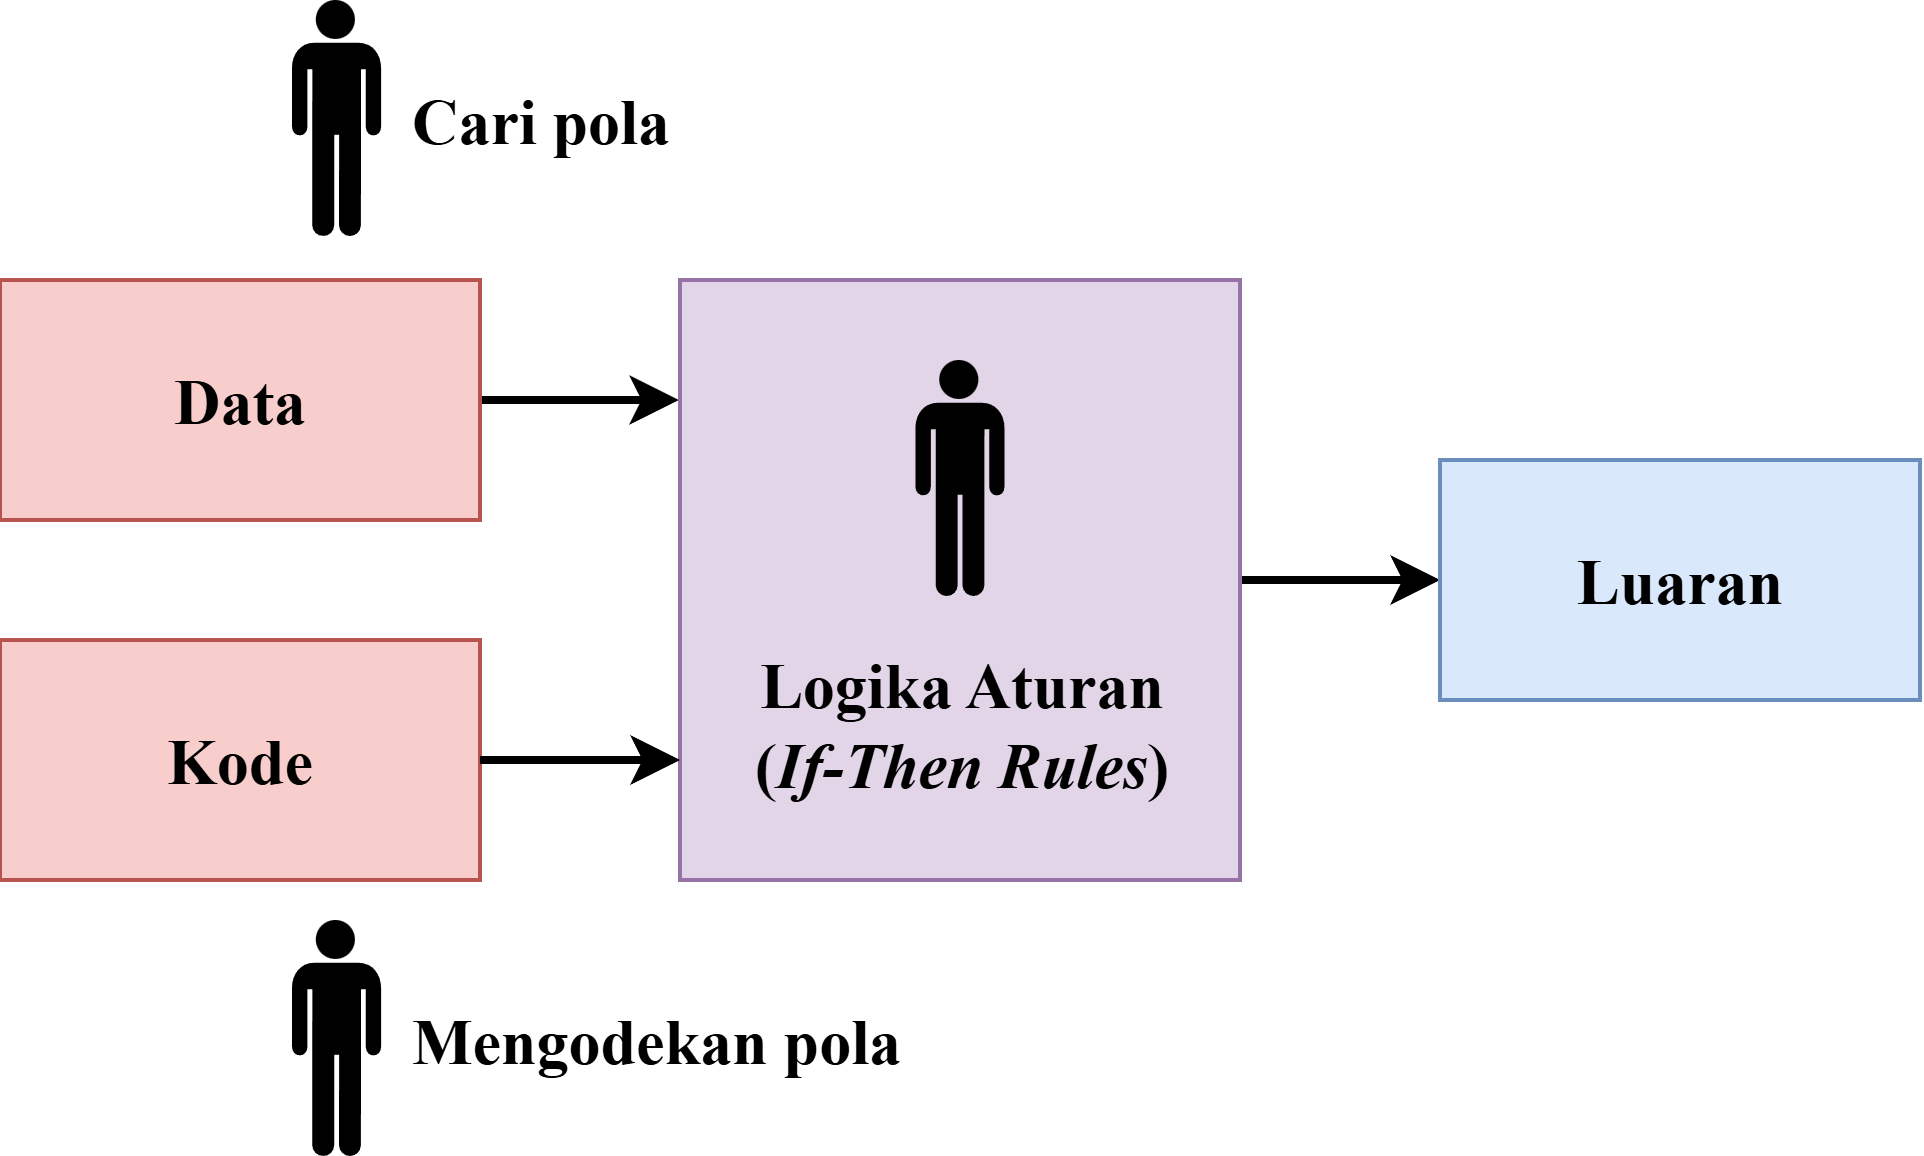
\includegraphics[width=\textwidth]{bab2/rulebasedsystem.png}
    \caption{}
    \label{fig:rule_based}
\end{subfigure}
\vspace{0.5cm}
\begin{subfigure}[b]{0.8\textwidth}
    \centering
    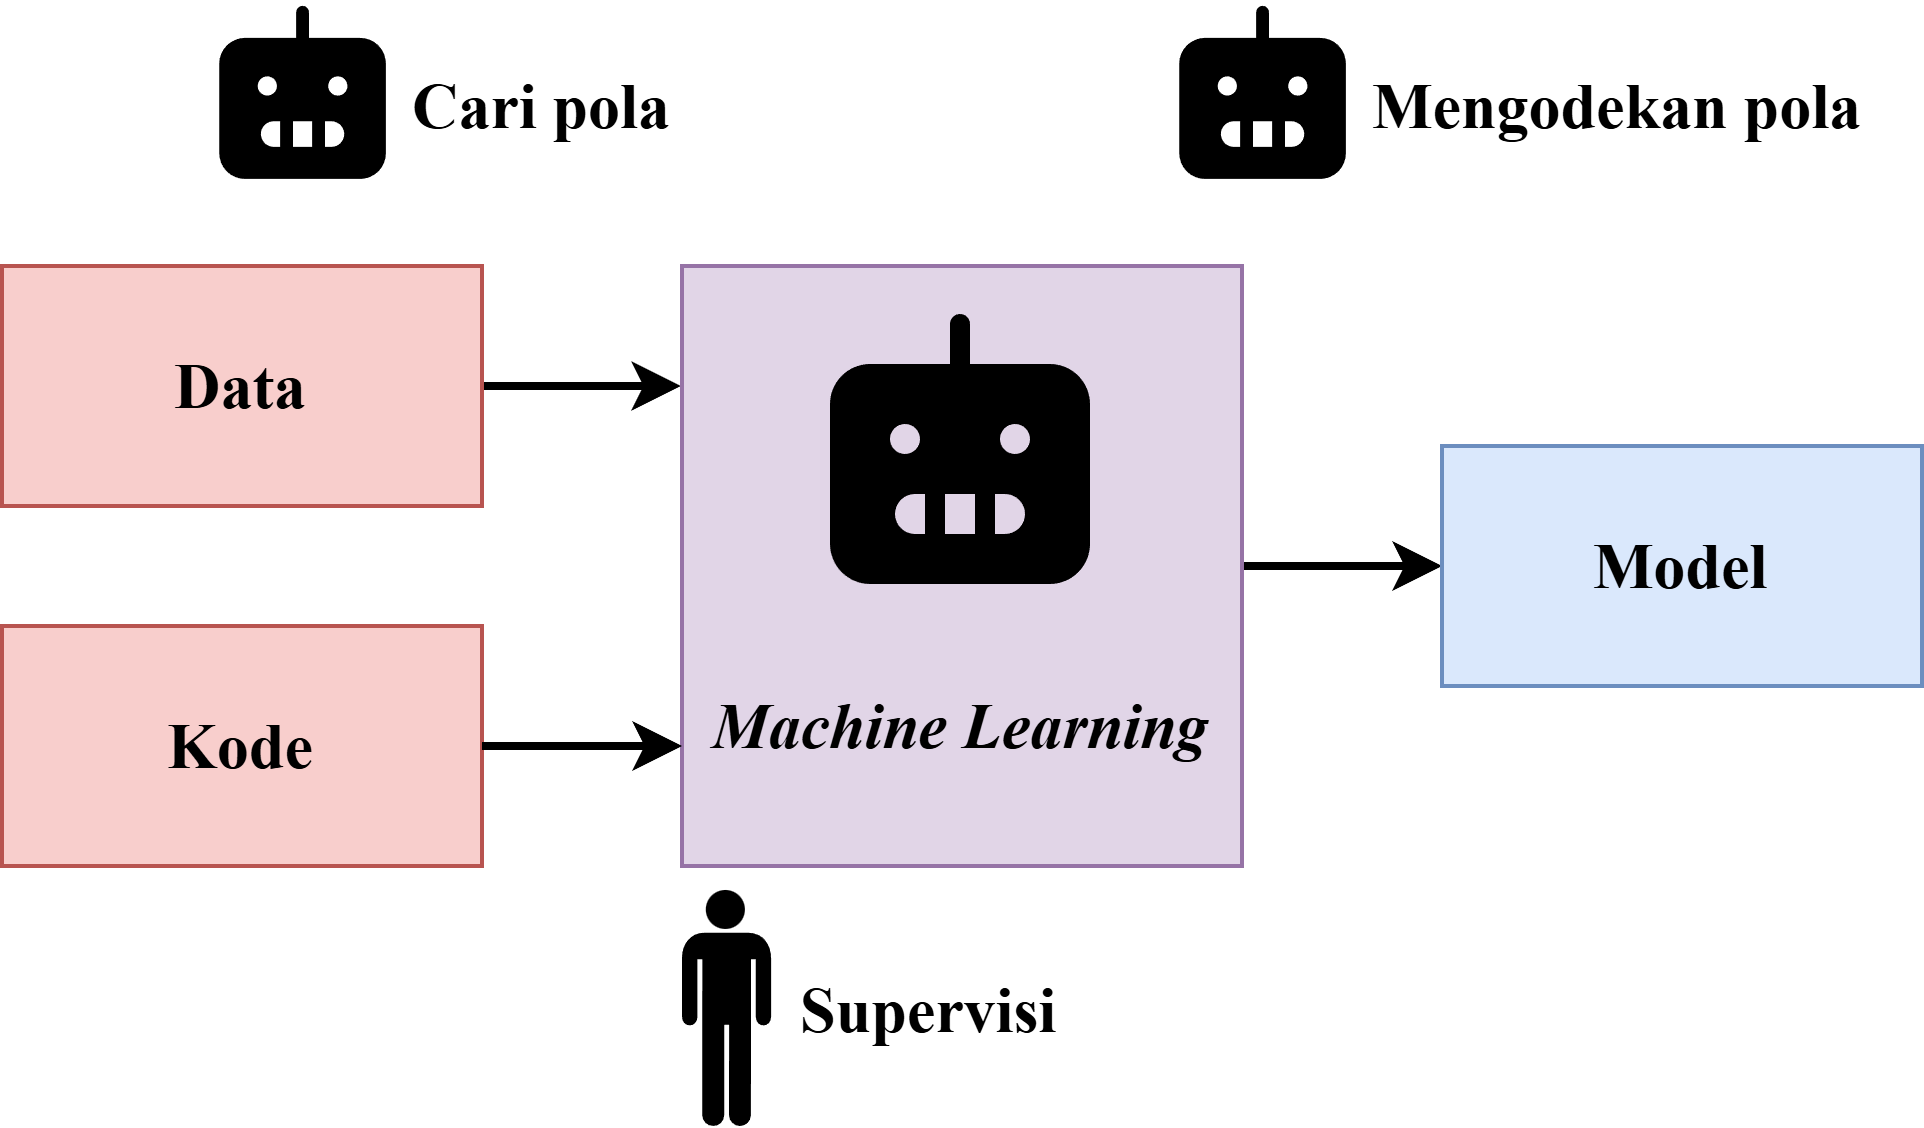
\includegraphics[width=\textwidth]{bab2/learningbasedsystem.png}
    \caption{}
    \label{fig:learning_based}
\end{subfigure}
\caption[Perbandingan paradigma \textit{rule-based system} dan \textit{machine learning system}]{Perbandingan paradigma \textit{rule-based system} dan \textit{machine learning system}: (a) \textit{Rule-based system} memproses data berdasarkan aturan untuk menghasilkan jawaban, sedangkan (b) \textit{Machine learning system} mempelajari aturan dari data dan jawaban yang diberikan.}
\label{fig:comparison_rule_learning}
\end{figure}

Sistem \textit{machine learning} dilatih dengan dihadapkan pada banyak contoh yang relevan, di mana ia menemukan struktur statistik yang memungkinkannya membuat aturan untuk mengotomatisasi tugas \parencite{cholletDeepLearningPython2026}. Fleksibilitas ini menjadi kunci dalam aplikasi praktis seperti identifikasi penyakit tanaman, di mana karakteristik visual gejala seringkali terlalu kompleks untuk dipetakan secara manual ke dalam aturan logika yang kaku \parencite{pacalSystematicReviewDeep2024}. Untuk mengoptimalkan proses akuisisi pengetahuan tersebut, algoritma \textit{machine learning} dikembangkan ke dalam berbagai metode yang disesuaikan dengan karakteristik data yang tersedia.

Secara umum, algoritma \textit{machine learning} dikelompokkan ke dalam empat kategori utama berdasarkan jenis data dan metode pembelajarannya \parencite{sarkerMachineLearningAlgorithms2021}. Visualisasi dari kategori-kategori tersebut disajikan pada Gambar \ref{fig:taxonomy_ml}. Keempat kategori tersebut dijabarkan sebagai berikut:
\begin{enumerate}[nosep]
    \item \textit{Supervised Learning}: Pendekatan di mana model dilatih menggunakan \textit{dataset} yang memiliki label eksplisit, yang terdiri dari pasangan masukan dan luaran yang benar. Tujuannya adalah untuk memetakan fungsi dari masukan ke luaran sehingga model dapat melakukan prediksi atau klasifikasi pada data baru yang belum pernah dilihat sebelumnya.
    \item \textit{Unsupervised Learning}: Pendekatan ini bekerja pada data yang tidak memiliki label atau anotasi sebelumnya. Fokus utamanya adalah untuk menemukan struktur, pola, atau hubungan tersembunyi di dalam data tanpa adanya panduan luaran yang spesifik, seperti pada tugas klasterisasi atau asosiasi.
    \item \textit{Semi-supervised Learning}: Kategori ini merupakan hibrida yang memanfaatkan \textit{dataset} berlabel dalam jumlah kecil bersama dengan \textit{dataset} tidak berlabel dalam jumlah besar selama proses pelatihan. Pendekatan ini dapat digunakan dalam skenario di mana biaya anotasi data oleh pakar sangat mahal, namun data mentah tersedia secara melimpah.
    \item \textit{Reinforcement Learning}: Metode pembelajaran yang berbasis pada interaksi agen dengan lingkungan melalui mekanisme \textit{reward} (penghargaan) dan \textit{penalty} (hukuman). Agen belajar untuk mengambil serangkaian tindakan yang dapat memaksimalkan akumulasi \textit{reward} dalam jangka panjang melalui proses \textit{trial and error}.
\end{enumerate}


\begin{figure}[H]
\centering
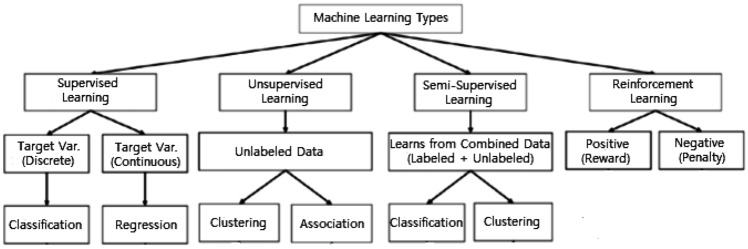
\includegraphics[width=0.8\textwidth]{bab2/kategoriml.png}
\caption[Ragam teknik \textit{machine learning}]{Ragam teknik \textit{machine learning} \parencite{sarkerMachineLearningAlgorithms2021}}
\label{fig:taxonomy_ml}
\end{figure}

% [TODO: MENTION ABOUT SELF-SUPERVISED LEARNING AS A SUBSET OF SUPERVISED LEARNING]

\section{\textit{Deep Learning}}
\textit{Deep learning} merupakan subbidang dari \textit{machine learning} yang menggunakan arsitektur \textit{artificial neural networks} (jaringan saraf tiruan) dengan banyak lapisan tersembunyi untuk mempelajari representasi data secara hierarkis \parencite{cholletDeepLearningPython2026,goodfellowDeepLearning2016, russell2020artificial}. Secara taksonomi, \textit{deep learning} merupakan bagian integral dari \textit{machine learning}, yang mana \textit{machine learning} itu sendiri berada di bawah payung besar AI. Hubungan hierarkis ini dapat divisualisasikan pada Gambar \ref{fig:hierarchy_ai_ml_dl}.
%NOTE: COPYRIGHT RED
\begin{figure}[H] 
\centering
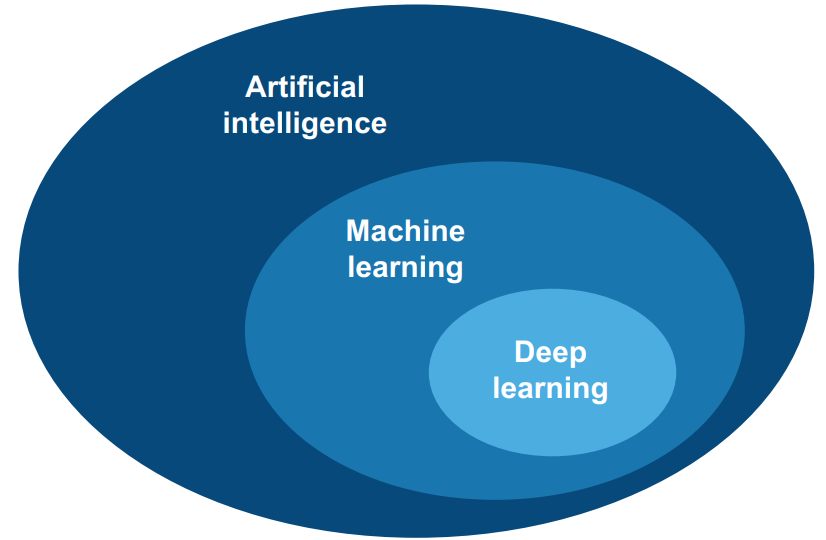
\includegraphics[width=0.45\textwidth]{bab2/hierarkiai.png}
\caption[Hierarki antara \textit{artificial intelligence}, \textit{machine learning}, \textit{representation learning}, dan \textit{deep learning}]{Hierarki antara \textit{artificial intelligence}, \textit{machine learning}, dan \textit{deep learning} \parencite{cholletDeepLearningPython2026}}
\label{fig:hierarchy_ai_ml_dl}
\end{figure}

\textit{Artificial neural networks} (ANN) merupakan fondasi utama dari \textit{deep learning} yang terinspirasi oleh struktur biologis otak manusia untuk memproses informasi melalui unit-unit komputasi yang saling terhubung \parencite{sarkerDeepLearningComprehensive2021}. Unit dasar dalam ANN adalah neuron yang menerima sinyal masukan, memberikan bobot dan bias tertentu, serta menerapkan fungsi aktivasi untuk menghasilkan luaran. Arsitektur dasar sebuah jaringan saraf terdiri dari tiga jenis lapisan utama, yaitu lapisan masukan, satu atau lebih lapisan tersembunyi, dan lapisan luaran. Secara spesifik, lapisan masukan berfungsi meneruskan data mentah ke dalam jaringan, sedangkan lapisan tersembunyi bertugas melakukan transformasi fitur melalui operasi bobot dan fungsi non-linear. Peningkatan jumlah lapisan tersembunyi akan memperdalam arsitektur jaringan, yang memungkinkan model untuk mempelajari hierarki representasi data yang lebih kompleks. Selanjutnya, hasil pemrosesan tersebut dikonversi oleh lapisan luaran menjadi nilai probabilitas atau prediksi akhir. Struktur jaringan saraf dan mekanisme operasional pada tingkat neuron diilustrasikan pada Gambar \ref{fig:nn_architecture}.

\begin{figure}[H] 
\centering
\begin{subfigure}[b]{0.8\textwidth}
    \centering
    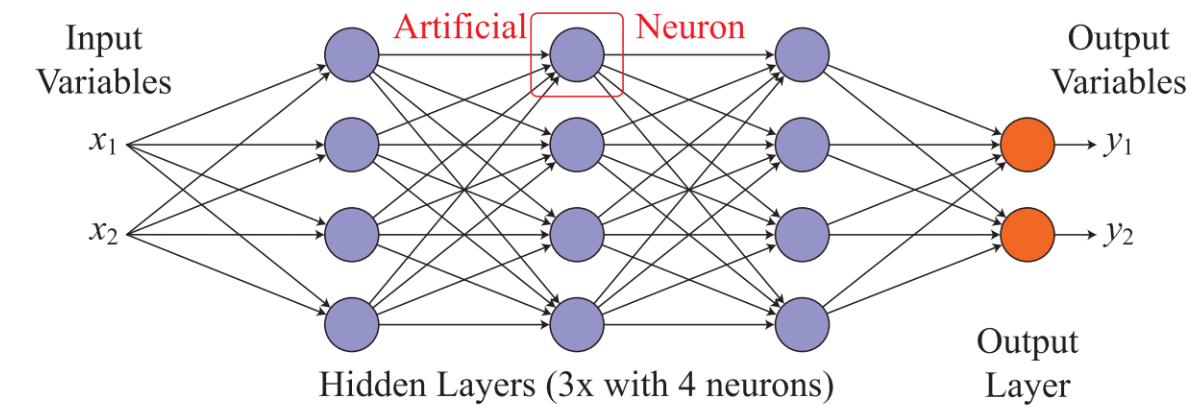
\includegraphics[width=\textwidth]{bab2/ann.png}
    \caption{}
\end{subfigure}
\vspace{0.5cm}
\begin{subfigure}[b]{\textwidth}
    \centering
    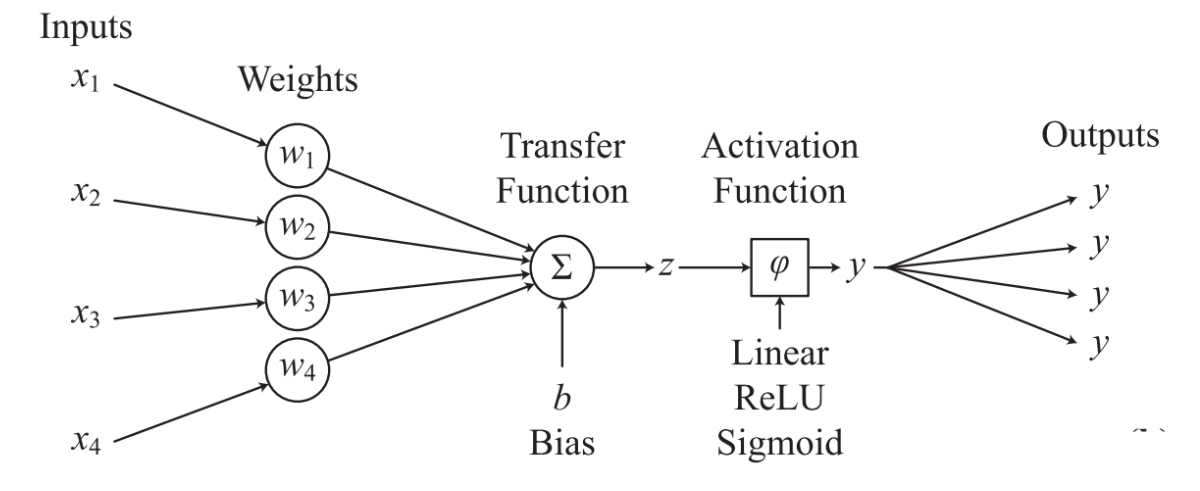
\includegraphics[width=\textwidth]{bab2/neuron.png}
    \caption{}
\end{subfigure}
\caption[Arsitektur jaringan saraf tiruan dan mekanisme kerja neuron]{Arsitektur jaringan saraf tiruan: (a) Hierarki lapisan pada ANN dan (b) Mekanisme matematis pada tingkat neuron \parencite{guillodArtificialNeuralNetwork2020}}
\label{fig:nn_architecture}
\end{figure}

Mekanisme pembelajaran pada model \textit{deep learning} berfokus pada pencarian sekumpulan nilai \textit{weights} (bobot) yang mampu memetakan masukan ke target yang benar secara akurat \parencite{cholletDeepLearningPython2026}. Spesifikasi transformasi data pada setiap lapisan ditentukan oleh bobot-bobot ini. Selama proses pelatihan, kualitas prediksi model ($Y'$) diukur menggunakan \textit{loss function} (fungsi kerugian) yang membandingkannya dengan target sebenarnya ($Y$) untuk menghasilkan skor kerugian (\textit{loss score}). Skor ini bertindak sebagai sinyal umpan balik yang mengindikasikan seberapa jauh penyimpangan model dari kinerja ideal. Informasi tersebut kemudian digunakan oleh \textit{optimizer} untuk memodifikasi nilai-nilai bobot melalui algoritma \textit{Backpropagation}, dengan tujuan meminimalkan skor kerugian pada iterasi berikutnya. Siklus iteratif yang terdiri dari prediksi, pengukuran kesalahan, dan penyesuaian bobot ini dikenal sebagai \textit{training loop}, yang terus dijalankan hingga model mencapai performa yang diharapkan. Proses pembelajaran ini divisualisasikan pada Gambar \ref{fig:dl_learning_process}.
% #NOTE: COPYRIGHT RED
\begin{figure}[H]
\centering
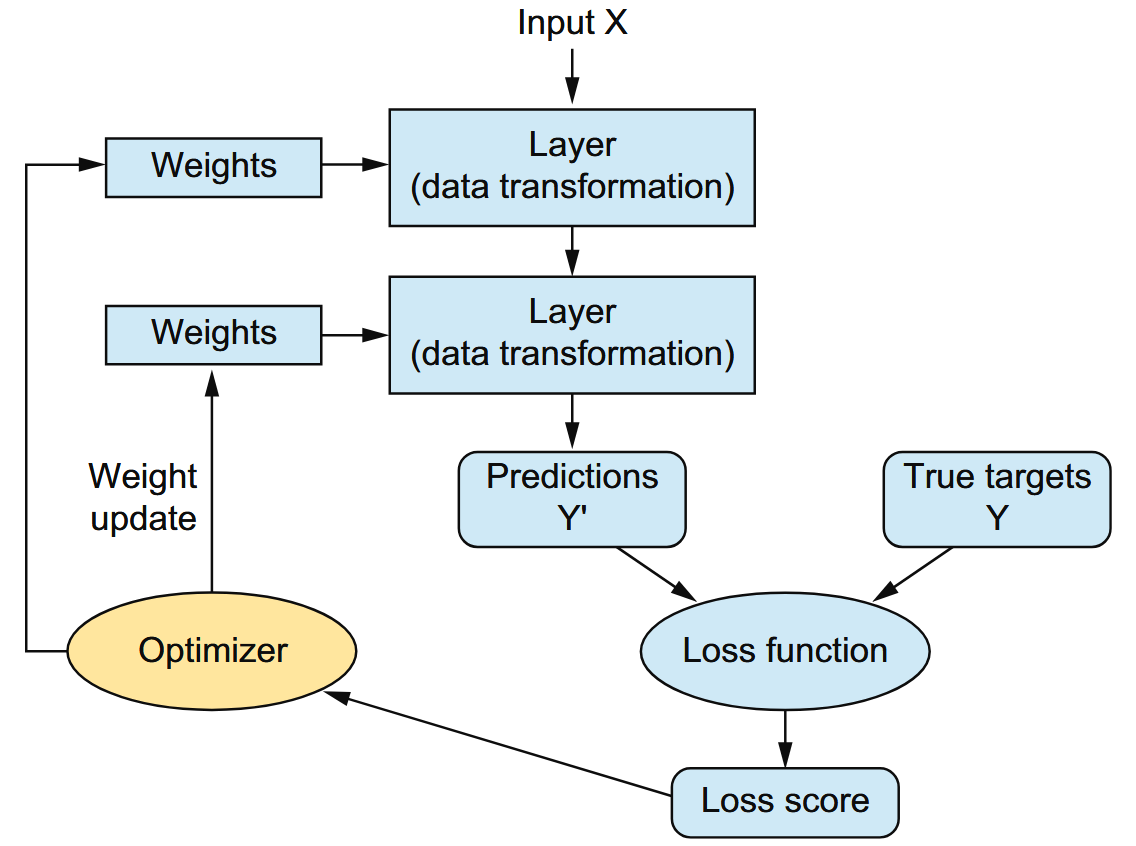
\includegraphics[width=0.7\textwidth]{bab2/dllearning.png}
\caption[Mekanisme pembelajaran pada model \textit{deep learning}]{Mekanisme pembelajaran pada model \textit{deep learning} \parencite{cholletDeepLearningPython2026}}
\label{fig:dl_learning_process}
\end{figure} 

Dalam perkembangannya, teknik-teknik \textit{deep learning} dapat dikategorikan berdasarkan karakteristik pembelajaran dan aplikasinya. \textcite{sarkerDeepLearningComprehensive2021} mengajukan taksonomi yang membagi teknik \textit{deep learning} ke dalam tiga kategori utama, yaitu \textit{supervised} atau \textit{discriminative learning}, \textit{unsupervised} atau \textit{generative learning}, serta \textit{hybrid learning}. Pembelajaran diskriminatif berfokus pada penyediaan fungsi pembeda untuk tugas klasifikasi terawasi, dengan arsitektur populer seperti \textit{Multi-Layer Perceptron} (MLP), \textit{Convolutional Neural Networks} (CNN), dan \textit{Recurrent Neural Networks} (RNN). Di sisi lain, pembelajaran generatif digunakan untuk mengekstraksi fitur korelasi tingkat tinggi atau sintesis data tanpa label, yang mencakup metode seperti \textit{Generative Adversarial Networks} (GAN), \textit{Autoencoders} (AE), dan \textit{Deep Belief Networks} (DBN). Kategori terakhir, pembelajaran hibrida, mengintegrasikan kedua pendekatan tersebut untuk menggabungkan keunggulan model generatif dan diskriminatif dalam menyelesaikan masalah yang lebih kompleks. Visualisasi taksonomi teknik \textit{deep learning} ini disajikan pada Gambar \ref{fig:dl_technique}.

\begin{figure}[H]
\centering
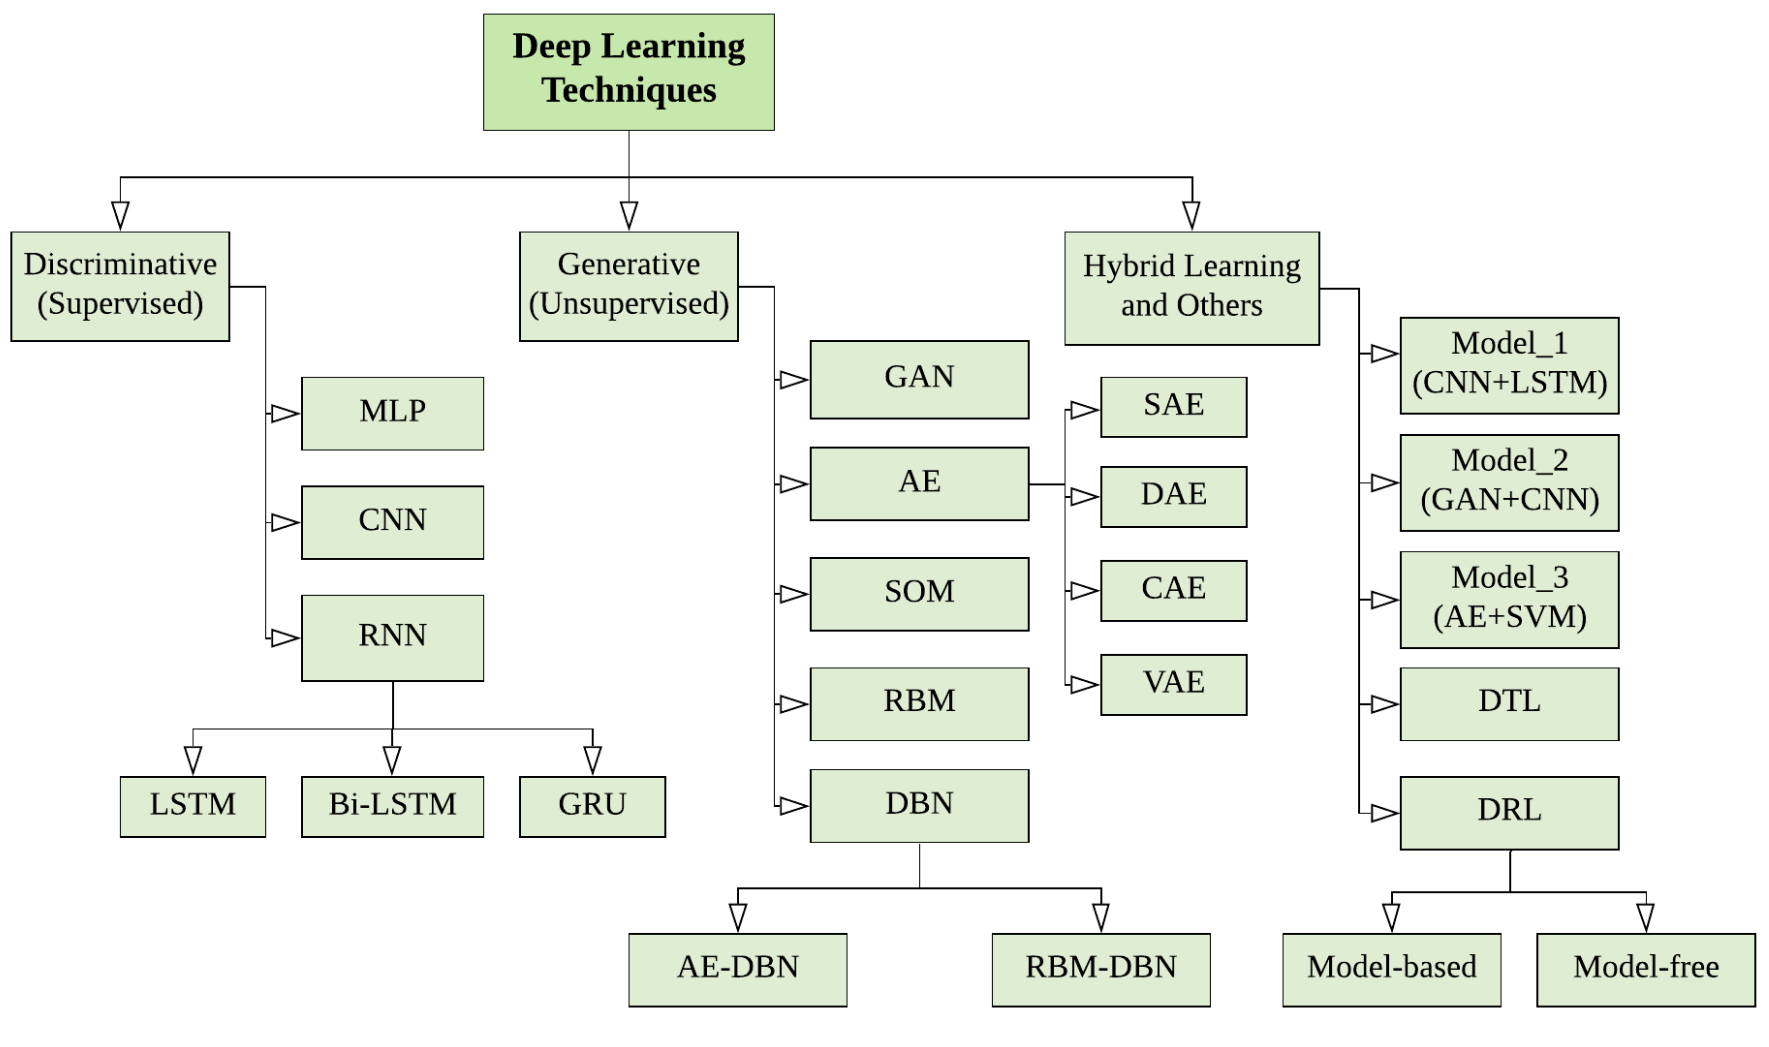
\includegraphics[width=\textwidth]{bab2/dltechnique.png}
\caption[Taksonomi teknik \textit{deep learning}]{Taksonomi teknik \textit{deep learning} \parencite{sarkerDeepLearningComprehensive2021}}
\label{fig:dl_technique}
\end{figure}

Perbedaan utama antara \textit{machine learning} tradisional dan \textit{deep learning} terletak pada cara fitur data diperoleh \parencite{goodfellowDeepLearning2016}. Fitur data dapat didefinisikan sebagai atribut atau karakteristik spesifik yang diekstraksi dari data mentah untuk merepresentasikan informasi penting bagi model. Goodfellow dkk. menjelaskan bahwa \textit{machine learning} tradisional sangat bergantung pada proses \textit{feature extraction} (ekstraksi fitur) secara manual yang membutuhkan pengetahuan domain mendalam. Untuk mengatasi ketergantungan tersebut, dikembangkan pendekatan \textit{representation learning} (pembelajaran representasi) yang otomatis menemukan representasi data yang diperlukan untuk menyelesaikan tugas tertentu. \textit{Deep learning} merupakan bentuk spesifik dari \textit{representation learning} yang mampu mengekstraksi fitur secara otomatis langsung dari data mentah melalui struktur lapisan hierarkis yang merepresentasikan konsep secara bertingkat dari ANN. 

Secara konseptual, kedalaman dalam arsitektur ini memungkinkan komputer untuk mempelajari konsep yang rumit dengan membangunnya dari konsep-konsep yang lebih sederhana \parencite{goodfellowDeepLearning2016}. Sebagai contoh dalam pengolahan citra, lapisan awal jaringan dapat mempelajari deteksi tepian, lapisan menengah mempelajari kontur atau sudut, dan lapisan akhir mengenali bagian objek yang spesifik. Hierarki fitur ini terbentuk secara otomatis selama proses pelatihan tanpa intervensi manusia. Hal ini menjadi keunggulan utama dibandingkan metode tradisional, karena sistem dapat mengadaptasi ekstraksi fiturnya sendiri sesuai dengan karakteristik data yang spesifik. Perbandingan alur pengolahan data ini disajikan dalam Gambar \ref{fig:workflow_ml_dl}.

\begin{figure}[H] 
\centering
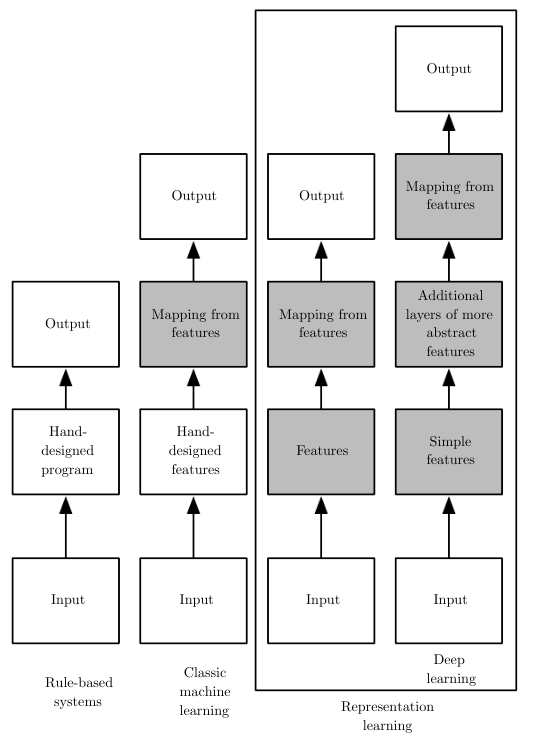
\includegraphics[max width=\textwidth, max height=0.6\textheight]{bab2/traditionalvsdeeplearning.png}
\caption[Perbandingan alur kerja antara \textit{machine learning} tradisional, \textit{representation learning}, dan \textit{deep learning}]{Perbandingan alur kerja antara \textit{machine learning} tradisional, \textit{representation learning}, dan \textit{deep learning} \parencite{goodfellowDeepLearning2016}}
\label{fig:workflow_ml_dl}
\end{figure}

Dalam implementasi \textit{deep learning}, terdapat konsep yang sering dikenal dengan \textit{pre-training}, di mana model dilatih terlebih dahulu pada \textit{dataset} berskala besar untuk mempelajari fitur umum sebelum diterapkan pada tugas yang lebih spesifik melalui \textit{transfer learning} \parencite{cholletDeepLearningPython2026}. Chollet menjelaskan bahwa fitur pada lapisan awal cenderung bersifat umum (\textit{general}), sementara fitur pada lapisan akhir lebih spesifik terhadap \textit{dataset} pelatihan asli. Oleh karena itu, terdapat dua strategi \textit{transfer learning} yang umum digunakan dalam pengembangan model \textit{deep learning}, yaitu \textit{feature extraction} dan \textit{fine-tuning}. Perbedaan mekanisme antara kedua strategi tersebut diilustrasikan pada Gambar \ref{fig:transfer_learning_mechanisms}.

\begin{figure}[H]
\centering
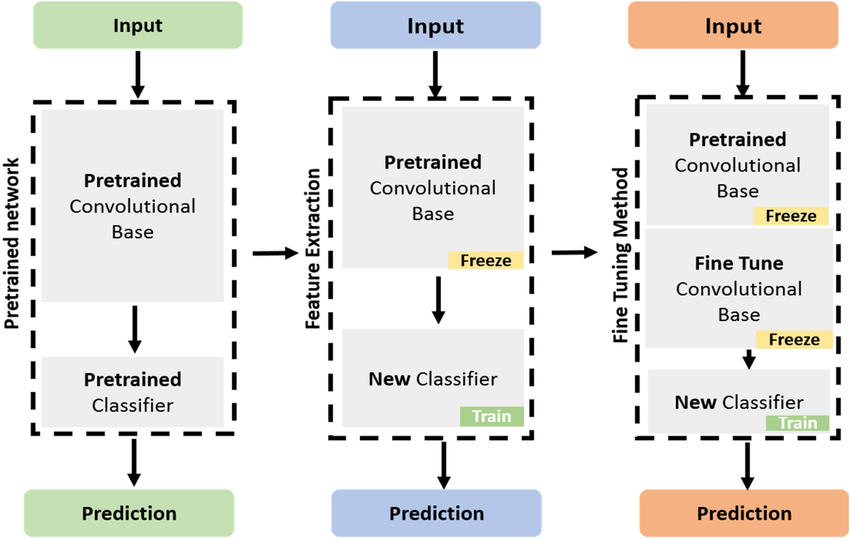
\includegraphics[width=\textwidth]{bab2/transferlearningmechanisms.png}
\caption[Contoh mekanisme \textit{feature extraction} dan \textit{fine-tuning} pada model CNN]{Contoh mekanisme \textit{feature extraction} dan \textit{fine-tuning} pada model CNN \parencite{asifDeepLearningbasedFramework2022}}
\label{fig:transfer_learning_mechanisms}
\end{figure}

Strategi \textit{feature extraction} bekerja dengan menggunakan bobot model yang sudah dilatih sebagai ekstraktor fitur tetap tanpa melakukan pembaruan bobot pada lapisan dasar model, sehingga hanya lapisan klasifikasi terakhir yang dilatih ulang \parencite{cholletDeepLearningPython2026}. Strategi ini ideal digunakan ketika \textit{dataset} target berukuran kecil atau memiliki kemiripan visual yang sangat tinggi dengan \textit{dataset} asal. Sebaliknya, strategi \textit{fine-tuning} melibatkan pelatihan kembali sebagian atau seluruh lapisan model menggunakan \textit{dataset} target dengan laju pembelajaran (\textit{learning rate}) yang lebih rendah guna mengadaptasi fitur yang sudah dipelajari ke domain data yang baru. Strategi ini lebih cocok diterapkan pada \textit{dataset} target yang berukuran besar atau memiliki karakteristik data yang berbeda secara signifikan dari \textit{dataset} asal.

Sebagian besar model \textit{deep learning} secara tradisional dilatih menggunakan pendekatan \textit{supervised learning} \parencite{goodfellowDeepLearning2016}. Momentum kebangkitan \textit{deep learning} modern pun dipicu oleh keberhasilan arsitektur AlexNet dari \textcite{krizhevskyImageNetClassificationDeep2017} yang dilatih secara supervisi untuk mengklasifikasikan citra pada \textit{dataset} ImageNet. Kendati demikian, \textcite{huyenAIEngineeringBuilding2025} memaparkan bahwa ketergantungan pada supervisi menghadirkan hambatan skalabilitas yang signifikan karena proses pelabelan data secara manual membutuhkan waktu dan biaya yang tinggi. Beban biaya ini akan meningkat seiring dengan bertambahnya jumlah kategori objek yang ingin dicakup oleh model. Selain itu, terdapat variabilitas dalam tingkat kesulitan pelabelan, yaitu meskipun pelabelan objek umum relatif murah, pelabelan pada domain spesifik yang menuntut kepakaran khusus memerlukan sumber daya yang jauh lebih besar.

Untuk mengatasi hambatan pelabelan data tersebut, dikembangkan paradigma \textit{self-supervised learning}. Dalam pendekatan ini, model tidak memerlukan label eksplisit, melainkan menginferensi label secara mandiri langsung dari informasi yang terkandung dalam data masukan. Kemampuan tersebut menjadi fondasi krusial bagi pengembangan \textit{foundation models} yang mampu mengintegrasikan berbagai modalitas data. Perkembangan ini yang kemudian melahirkan \textit{Vision-Language Models}, yang menggabungkan kemampuan pemahaman visual dan tekstual secara sinergis untuk menyelesaikan tugas-tugas penalaran yang kompleks \parencite{bordesIntroductionVisionLanguageModeling2024}. Pendekatan ini menjadi sangat relevan dalam mengatasi tantangan kelangkaan data berlabel pada domain-domain spesifik, termasuk dalam identifikasi penyakit tanaman yang memerlukan anotasi dari pakar.

% Note: Ini versi lama. Disimpan untuk referensi saja.
% Walaupun \textit{deep learning} menawarkan keunggulan dalam akurasi, model ini secara tradisional sangat bergantung pada ketersediaan data berlabel dalam jumlah besar terutama untuk pelatihan berbasis \textit{supervised learning} \parencite{goodfellowDeepLearning2016}. Keterbatasan ini mendorong perkembangan paradigma \textit{self-supervised learning}, di mana model dirancang untuk mempelajari representasi data dari data yang tidak berlabel dengan cara menciptakan tugas prediksi internal dari struktur data itu sendiri \parencite{minaeeLargeLanguageModels2025}. Paradigma ini memungkinkan pemanfaatan data dalam skala masif untuk membangun representasi fitur yang kaya tanpa bergantung pada anotasi manusia yang mahal. Kemampuan tersebut menjadi fondasi krusial bagi pengembangan \textit{foundation models} yang mampu mengintegrasikan berbagai modalitas data. Perkembangan ini yang kemudian melahirkan \textit{Vision-Language Models}, yang menggabungkan kemampuan pemahaman visual dan tekstual secara sinergis untuk menyelesaikan tugas-tugas penalaran yang kompleks \parencite{bordesIntroductionVisionLanguageModeling2024}. Pendekatan ini menjadi sangat relevan dalam mengatasi tantangan kelangkaan data berlabel pada domain-domain spesifik, termasuk dalam identifikasi penyakit tanaman yang memerlukan anotasi dari pakar.

\section{\textit{Large-Language Models}}
\textit{Large Language Models} (LLM) merupakan salah satu terobosan paling signifikan dalam bidang \textit{Natural Language Processing} (NLP) \parencite{cholletDeepLearningPython2026}. NLP didefinisikan sebagai subbidang AI yang berfokus pada pengembangan algoritma untuk memproses, memahami, serta menghasilkan bahasa alami manusia, baik dalam bentuk teks maupun suara \parencite{jm3}. Dalam hierarki teknologi, LLM menempati posisi sebagai model bahasa tingkat lanjut yang memanfaatkan teknik \textit{deep learning} untuk memproses informasi tekstual dalam skala yang sangat besar.

\begin{figure}[H]
\centering
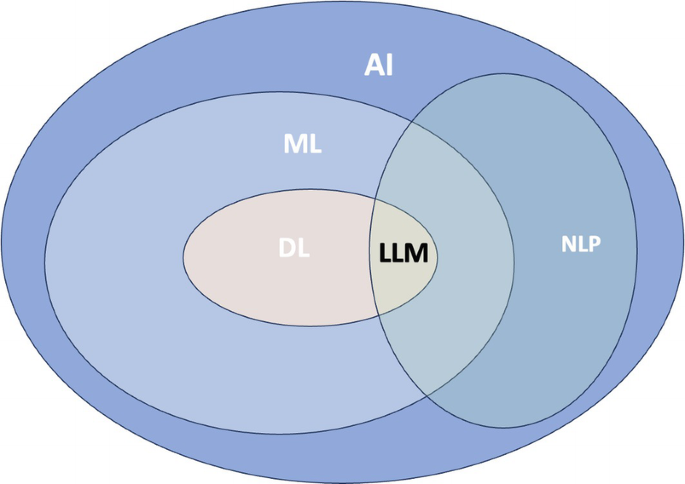
\includegraphics[width=0.6\textwidth]{bab2/llmnlp.png}
\caption[Hubungan antara AI, NLP, dan LLM]{Hubungan antara AI, NLP, dan LLM \parencite{Bottino2024}}
\label{fig:ai_ml_dl_llm}
\end{figure}

Terminologi LLM terdiri dari dua komponen utama, yakni model bahasa (\textit{language model}) dan skala besar (\textit{large}). Model bahasa berfungsi untuk mengodekan informasi statistik mengenai satu atau lebih bahasa \parencite{huyenAIEngineeringBuilding2025}. Secara intuitif, informasi ini mengindikasikan seberapa besar kemungkinan suatu kata muncul dalam konteks tertentu. Dari sini, model bahasa dapat memprediksi kata yang paling mungkin muncul berikutnya dalam suatu \textit{sequence} (urutan) berdasarkan konteks yang diberikan. Mekanisme prediksi kata berikutnya ini memanfaatkan sifat sekuensial alami bahasa untuk melatih model agar mampu memahami konteks, struktur, serta hubungan antar elemen di dalam teks \parencite{raschkaBuildLargeLanguage2025}. Karena kemampuannya dalam membangkitkan teks tersebut, LLM juga sering diklasifikasikan sebagai bentuk kecerdasan buatan generatif (\textit{generative AI} atau \textit{GenAI}). Terminologi ini merujuk pada kemampuan model untuk menghasilkan luaran yang bersifat terbuka (\textit{open-ended}), di mana kosakata yang terbatas digunakan untuk mengonstruksi kemungkinan luaran yang tak terbatas \parencite{huyenAIEngineeringBuilding2025}.

% NOTE: Ini versi lama. Disimpan untuk referensi saja.
% Model bahasa secara fundamental adalah model probabilitas berbasis jaringan saraf yang menerima masukan berupa konteks atau prefiks teks, dan menghasilkan distribusi probabilitas terhadap kata atau token berikutnya yang paling mungkin muncul. Ilustrasi mekanisme dasar LLM sebagai model prediksi urutan kata disajikan pada Gambar \ref{fig:llm_illustration}. 
% \begin{figure}[H]
% \centering
% \includegraphics[width=0.8\textwidth]{bab2/llmilust.png}
% \caption[Ilustrasi mekanisme prediksi kata pada LLM]{Ilustrasi mekanisme LLM yang menerima konteks dan menghasilkan distribusi kata berikutnya \parencite{jm3}}
% \label{fig:llm_illustration}
% \end{figure}
Atribut "besar" pada LLM merujuk pada dua aspek utama, yaitu ukuran model dalam hal parameter serta \textit{dataset} masif yang digunakan sebagai basis pelatihannya \parencite{raschkaBuildLargeLanguage2025}. Model jenis ini umumnya memiliki puluhan hingga ratusan miliar parameter, yang merupakan bobot yang dapat disesuaikan dalam jaringan dan dioptimalkan selama pelatihan untuk memprediksi kata berikutnya dalam suatu urutan. Skala parameter ini berbanding lurus dengan kapasitas komputasi yang dibutuhkan, yang umumnya diukur dalam satuan FLOPS (\textit{Floating Point Operations per Second}) untuk merepresentasikan jumlah operasi aritmatika yang dilakukan per detik selama proses pelatihan maupun inferensi \parencite{amidiSuperStudyGuide2024}. Visualisasi mengenai korelasi antara jumlah parameter dan arsitektur model disajikan pada Gambar \ref{fig:model_parameters}.
\begin{figure}[H]
\centering
\includegraphics[width=0.8\textwidth]{bab2/modelparameters.png}
\caption[Visualisasi parameter pada model bahasa]{Visualisasi parameter pada model bahasa \parencite{amidiSuperStudyGuide2024}}
\label{fig:model_parameters}
\end{figure}
Perkembangan model bahasa modern saat ini hampir seluruhnya didasarkan pada arsitektur \textit{Transformer} yang diperkenalkan pertama kali oleh \textcite{vaswaniAttentionAllYou2023} melalui penelitian "Attention Is All You Need" \parencite{jm3,raschkaBuildLargeLanguage2025}. Arsitektur ini memperkenalkan mekanisme \textit{self-attention} yang memungkinkan model untuk memproses seluruh urutan kata secara paralel dan memahami ketergantungan antar kata terlepas dari jarak posisinya dalam kalimat. Inovasi ini menjadi fondasi utama bagi hampir seluruh LLM populer yang ada saat ini.

Dalam proses kerjanya, LLM mengandalkan mekanisme tokenisasi untuk memecah teks masukan menjadi unit-unit kecil yang disebut sebagai token \parencite{jm3}. Proses ini merupakan tahap fundamental pertama yang memungkinkan model untuk menginterpretasikan bahasa manusia ke dalam format yang dapat diproses secara komputasional. Terdapat berbagai strategi tokenisasi, mulai dari pemisahan berbasis kata, karakter, hingga sub-kata (\textit{sub-word}) seperti \textit{Byte-Pair Encoding} (BPE) yang mampu menangani kata-kata langka secara lebih efisien. Setelah melalui proses tokenisasi (\textit{encode}), urutan token tersebut dapat dikembalikan ke bentuk teks asli melalui proses sebaliknya (\textit{decode}), seperti yang diilustrasikan pada Gambar \ref{fig:encode_decode}.

\begin{figure}[H]
\centering
\includegraphics[width=1\textwidth]{bab2/encodedecode.png}
\caption[Mekanisme tokenisasi]{Mekanisme tokenisasi: (a) Proses \textit{encode} dari teks ke token dan (b) Proses \textit{decode} dari token ke teks \parencite{amidiSuperStudyGuide2024}}
\label{fig:encode_decode}
\end{figure}

Setiap token kemudian dikonversi menjadi representasi numerik dalam bentuk vektor dimensi tinggi yang dikenal sebagai \textit{embedding} \parencite{jm3}. Vektor-vektor ini ditempatkan dalam ruang fitur di mana kata-kata dengan makna serupa akan berada pada posisi yang berdekatan. Kedekatan atau kemiripan antar vektor tersebut umumnya diukur menggunakan teknik kesamaan vektor, seperti \textit{cosine similarity}, yang memungkinkan model untuk menangkap hubungan semantik antar token dalam dimensi ruang tertentu. Representasi ini memungkinkan model melakukan operasi aritmatika vektor untuk menangkap relasi analogi antar kata, seperti diilustrasikan pada Gambar \ref{fig:vector_representation}.

\begin{figure}[H]
\centering
\includegraphics[width=0.7\textwidth]{bab2/kingmanwomanqueen.png}
\caption[Visualisasi representasi vektor pada ruang \textit{embedding}]{Visualisasi representasi vektor pada ruang \textit{embedding} dengan contoh analogi $king - man + woman \approx queen$ oleh \textcite{mikolovEfficientEstimationWord2013} \parencite{sutorMetaconceptsIsolatingContext2019a}}
\label{fig:vector_representation}
\end{figure}

Kemampuan utama LLM dalam menghasilkan teks dilakukan melalui mekanisme \textit{autoregressive}, di mana model memprediksi token berikutnya berdasarkan urutan token sebelumnya secara berulang \parencite{jm3}. Visualisasi dari proses pembangkitan teks secara \textit{autoregressive} ini disajikan pada Gambar \ref{fig:llm_generation}. Proses pembangkitan ini dipandu oleh instruksi atau masukan teks awal yang disebut sebagai \textit{prompt}. Melalui konfigurasi \textit{prompt} yang tepat, model dapat diarahkan untuk menjalankan tugas-tugas tertentu tanpa memerlukan pembaruan parameter model secara permanen, sebuah fenomena yang dikenal sebagai \textit{in-context learning}.

\begin{figure}[H]
\centering
\includegraphics[width=0.8\textwidth]{bab2/llmgeneration.png}
\caption[Mekanisme pembangkitan teks autoregresif pada LLM]{Mekanisme pembangkitan teks autoregresif pada LLM \parencite{jm3}}
\label{fig:llm_generation}
\end{figure}

LLM dilatih melalui pendekatan \textit{self-supervised learning} \parencite{huyenAIEngineeringBuilding2025}. Pendekatan ini memungkinkan model untuk belajar dari urutan teks tanpa memerlukan pelabelan eksplisit, karena label diinferensi secara mandiri dari data masukan. Dalam konteks pemodelan bahasa, setiap urutan masukan menyediakan label berupa token yang akan diprediksi sekaligus konteks yang digunakan untuk melakukan prediksi tersebut. Mengingat ketersediaan urutan teks yang sangat melimpah, metode ini memungkinkan konstruksi data pelatihan dalam jumlah masif yang memfasilitasi peningkatan skala model bahasa menjadi LLM.

Meskipun memiliki kemampuan bahasa yang menyerupai manusia, LLM tetap memiliki batasan intrinsik berupa fenomena halusinasi \parencite{minaeeLargeLanguageModels2025}. Halusinasi merujuk pada kondisi di mana model menghasilkan informasi yang tampak masuk akal secara bahasa namun tidak memiliki dasar faktual atau tidak sesuai dengan data pelatihan yang ada. Hal ini karena LLM pada dasarnya bekerja sebagai model probabilitas yang memprediksi urutan kata yang paling mungkin, bukan sebagai sistem yang menyimpan pengetahuan faktual secara eksplisit. 

\textcite{minaeeLargeLanguageModels2025} mengidentifikasi berbagai metode augmentasi untuk mengurangi halusinasi pada LLM. Beberapa di antaranya adalah \textit{fine-tuning}, \textit{Retrieval-Augmented Generation} (RAG), penggunaan alat eksternal, serta pengembangan agen LLM. \textit{Fine-tuning} memungkinkan model beradaptasi dengan tugas tertentu melalui pelatihan ulang sebagian parameternya menggunakan data yang lebih kecil dan terkurasi. Akan tetapi, pendekatan ini menghadapi sejumlah kendala, seperti kebutuhan data pelatihan yang cukup besar, risiko terjadinya \textit{catastrophic forgetting} (hilangnya pengetahuan umum), serta tingginya biaya komputasi dalam pelatihan. Sebagai alternatif, RAG menawarkan solusi yang lebih fleksibel dengan menggabungkan LLM dan mekanisme pengambilan informasi dari sumber eksternal yang sudah disiapkan. Dengan cara ini, model dapat menghasilkan jawaban yang lebih relevan, akurat, dan dapat dipercaya.

Mekanisme pengambilan informasi eksternal ini, menurut \textcite{minaeeLargeLanguageModels2025}, merupakan salah satu contoh bagaimana LLM dapat menggunakan \textit{tools} (alat) eksternal. Alat eksternal ini pada dasarnya dapat berupa fungsi, API (\textit{Application Programming Interface}), atau layanan apa pun yang memberikan akses ke data dinamis, kalkulasi, atau kapabilitas lainnya. Lebih lanjut, kemampuan ini dapat ditingkatkan melalui konsep agen LLM yang dirancang untuk memungkinkan LLM menggunakan berbagai alat yang disediakan secara adaptif. 


\subsection{Arsitektur \textit{Transformer}}
Arsitektur \textit{Transformer} adalah arsitektur \textit{deep learning} yang pertama kali diperkenalkan oleh \textcite{vaswaniAttentionAllYou2023} untuk keperluan penerjemahan mesin (\textit{machine translation}).
Arsitektur ini awalnya digunakan untuk menerjemahkan teks bahasa Inggris ke bahasa Jerman dan Perancis \parencite{raschkaBuildLargeLanguage2025}. Kehadiran arsitektur ini kemudian membawa revolusi besar dalam bidang NLP serta berbagai tugas lain yang melibatkan pemetaan urutan-ke-urutan (\textit{sequence-to-sequence}) \parencite{altoBuildingLLMPowerd2024}. 

Secara fundamental, arsitektur \textit{Transformer} memanfaatkan mekanisme \textit{attention} untuk melakukan proses \textit{encode} dan \textit{decode} terhadap suatu urutan data \parencite{altoBuildingLLMPowerd2024}. Mekanisme ini hadir sebagai penyempurnaan dari metode sebelumnya yang diterapkan pada \textit{Recurrent Neural Networks} (RNN). Pada arsitektur RNN, pemrosesan data dilakukan secara sekuensial, di mana informasi diproses langkah demi langkah dengan meneruskan status tersembunyi (\textit{hidden state}) dari satu langkah ke langkah berikutnya. Pendekatan ini memiliki keterbatasan dalam menangkap hubungan ketergantungan jangka panjang. Sebaliknya, mekanisme \textit{attention} memungkinkan model untuk memusatkan perhatian pada bagian-bagian yang paling relevan dari urutan masukan saat menyusun luaran. 

Komponen utama yang menerapkan mekanisme ini dalam arsitektur \textit{Transformer} adalah lapisan \textit{Multi-Head Attention} \parencite{jm3}. Mekanisme ini sering juga disebut sebagai \textit{self-attention} karena diterapkan pada urutan yang sama dengan yang sedang dikodekan \parencite{altoBuildingLLMPowerd2024}. Secara sederhana, lapisan \textit{self-attention} bertugas untuk menentukan tingkat kepentingan dari setiap token masukan dalam hubungannya dengan token lain saat menghasilkan luaran. Dalam implementasinya, mekanisme \textit{self-attention} melibatkan tiga matriks bobot yang dipelajari selama pelatihan, yaitu \textit{Query} ($Q$), \textit{Key} ($K$), dan \textit{Value} ($V$). Di sini, $Q$ merepresentasikan token yang sedang diproses atau apa yang dicari, $K$ bertindak sebagai label identitas untuk setiap token dalam urutan atau apa yang tersedia, dan $V$ menyimpan konten informasi aktual dari token tersebut. Proses komputasi dimulai dengan menghitung skor atensi melalui perkalian $Q$ dan $K$ untuk menentukan seberapa relevan suatu token terhadap token lainnya. Skor ini kemudian dinormalisasi menggunakan fungsi \textit{Softmax} dan dikalikan dengan $V$ untuk menghasilkan vektor konteks yang telah diperkaya dengan informasi dari bagian input yang relevan. Mekanisme dekomposisi matriks input dan representasi operasi perkalian matriks ini diilustrasikan pada Gambar \ref{fig:attention_matrices}.

\begin{figure}[H]
\centering
\begin{subfigure}[b]{0.45\textwidth}
    \centering
    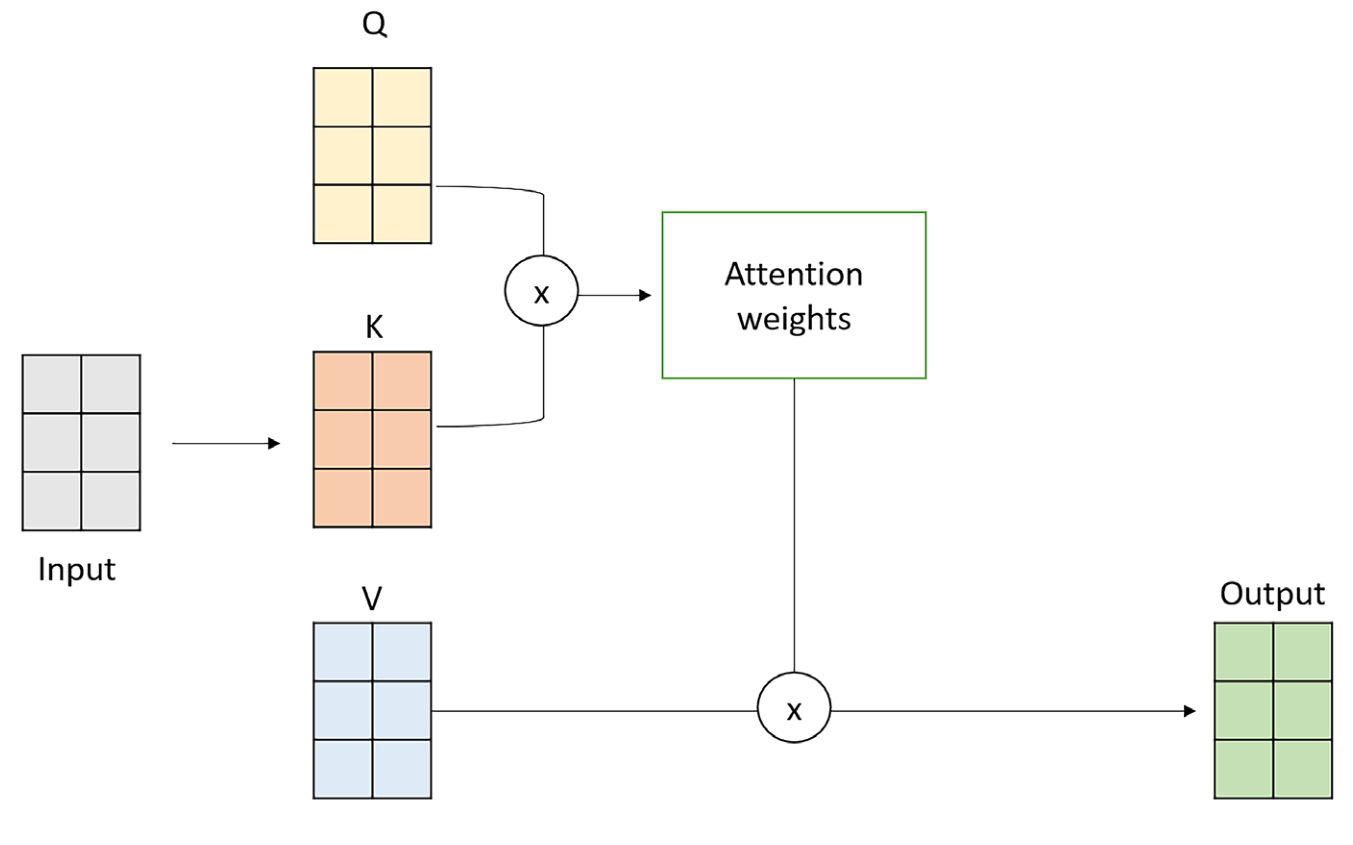
\includegraphics[width=\textwidth]{bab2/dekomposisimatriks.png}
    \caption{}
    \label{fig:dekomposisi_matriks}
\end{subfigure}
\hfill
\begin{subfigure}[b]{0.45\textwidth}
    \centering
    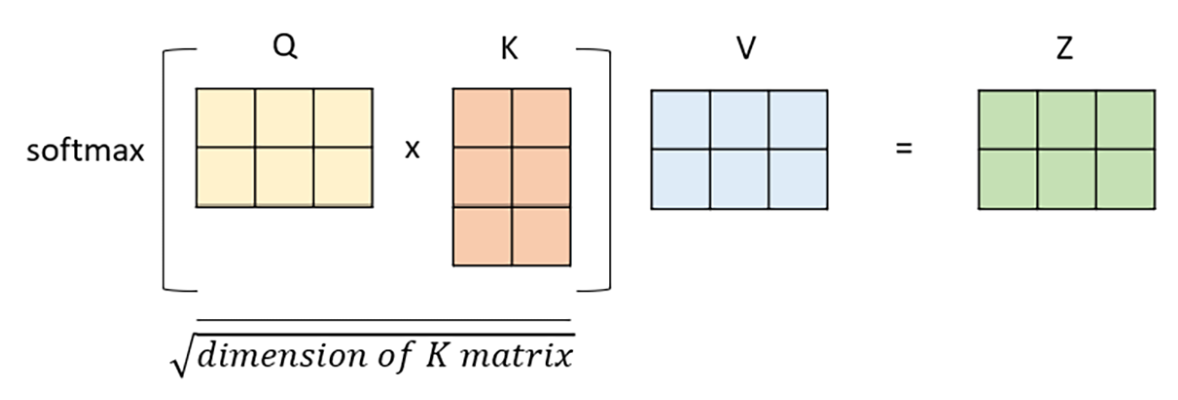
\includegraphics[width=\textwidth]{bab2/representasimatriks.png}
    \caption{}
    \label{fig:representasi_matriks}
\end{subfigure}
\caption[Dekomposisi dan representasi operasi matriks pada mekanisme \textit{self-attention}]{Dekomposisi dan representasi operasi matriks pada mekanisme \textit{self-attention}: (a) Dekomposisi matriks input menjadi vektor Q, K, dan V, serta (b) Representasi perkalian matriks Q, K, dan V untuk mendapatkan vektor konteks \parencite{altoBuildingLLMPowerd2024}}
\label{fig:attention_matrices}
\end{figure} 

Secara struktural, arsitektur \textit{Transformer} terdiri dari dua submodul utama, yakni pengode (\textit{encoder}) dan pendekode (\textit{decoder}) \parencite{raschkaBuildLargeLanguage2025}. Modul \textit{encoder} berfungsi untuk memproses teks masukan dan mengodekannya menjadi serangkaian representasi numerik atau vektor yang menangkap informasi kontekstual dari masukan tersebut. Selanjutnya, modul \textit{decoder} memanfaatkan vektor yang telah dikodekan ini untuk membangkitkan teks luaran. Dalam tugas penerjemahan bahasa, \textit{encoder} akan mengubah teks dari bahasa sumber menjadi representasi vektor, sedangkan \textit{decoder} akan menguraikan kode vektor tersebut untuk menghasilkan teks dalam bahasa target. Kedua modul ini tersusun atas lapisan-lapisan yang saling terhubung melalui mekanisme \textit{self-attention}. Keseluruhan arsitektur ini disajikan pada Gambar \ref{fig:transformer_architecture}.

\begin{figure}[H]
\centering
\includegraphics[max width=\linewidth, max totalheight=0.37\textheight, keepaspectratio]{bab1/arsitekturtransformer.png}
\caption[Arsitektur \textit{Transformer}]{Arsitektur \textit{Transformer} \parencite{vaswaniAttentionAllYou2023}}
\label{fig:transformer_architecture}
\end{figure}

Dalam pengembangannya, arsitektur \textit{encoder-decoder} dari \textcite{vaswaniAttentionAllYou2023} telah diadaptasi menjadi berbagai varian yang dioptimalkan untuk tugas-tugas spesifik. Adaptasi ini umumnya diklasifikasikan ke dalam tiga kategori utama berdasarkan bagian arsitektur yang digunakan, yaitu \textit{encoder-decoder}, \textit{encoder-only}, dan \textit{decoder-only} \parencite{amidiSuperStudyGuide2024}. Perbedaan struktur antara ketiga kategori arsitektur tersebut diilustrasikan pada Gambar \ref{fig:three_transformer_architectures}.

\begin{figure}[H]
\centering
\includegraphics[width=\textwidth]{bab2/tigaarsitekturtransformer.png}
\caption[Tiga varian arsitektur \textit{Transformer}]{Tiga varian arsitektur \textit{Transformer}: \textit{encoder-only}, \textit{encoder-decoder}, dan \textit{decoder-only} \parencite{jm3}}
\label{fig:three_transformer_architectures}
\end{figure}

BERT (\textit{Bidirectional Encoder Representations from Transformers}) dan GPT (\textit{Generative Pretrained Transformers}) merupakan contoh varian arsitektur \textit{Transformer} \parencite{raschkaBuildLargeLanguage2025}. BERT dibangun di atas submodul \textit{encoder} dari arsitektur asli \textit{Transformer}. Pendekatan pelatihannya berfokus pada prediksi kata yang disembunyikan atau \textit{masked word prediction}, di mana model memprediksi kata-kata yang ditutupi dalam suatu kalimat. Strategi ini memberikan BERT keunggulan dalam tugas-tugas klasifikasi teks, seperti prediksi sentimen dan kategorisasi dokumen. Di sisi lain, GPT berfokus pada bagian \textit{decoder} dari arsitektur \textit{Transformer} dan dirancang khusus untuk tugas-tugas generatif. Model ini menghasilkan teks kata demi kata dan mampu menangani berbagai tugas seperti penerjemahan mesin, peringkasan teks, hingga penulisan fiksi. Selain itu, model GPT juga menunjukkan kemampuan yang menonjol dalam melakukan \textit{zero-shot} dan \textit{few-shot learning}, yang memungkinkannya untuk menggeneralisasi tugas baru tanpa atau dengan sedikit contoh. Representasi visual dari perbedaan arsitektur \textit{encoder} pada BERT dan \textit{decoder} pada GPT dapat dilihat pada Gambar \ref{fig:bert_vs_gpt}.

\begin{figure}[H]
\centering
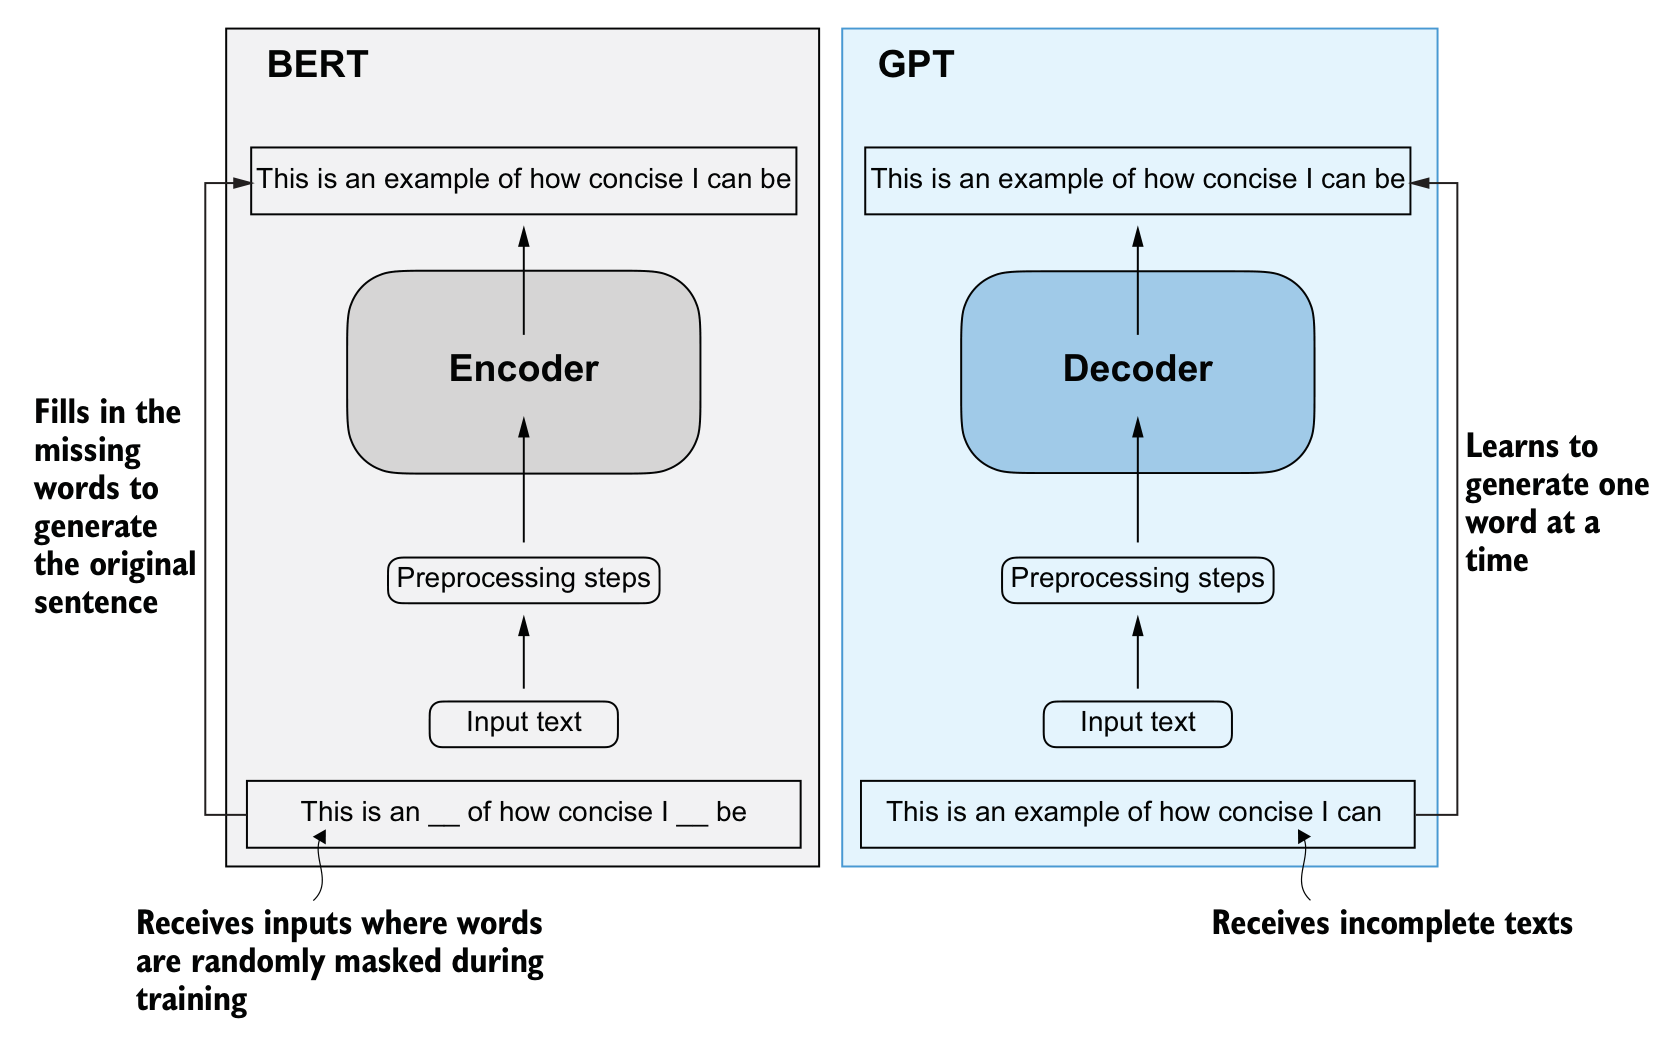
\includegraphics[max width=\linewidth, max totalheight=0.37\textheight, keepaspectratio]{bab2/encoderbertdecodergpt.png}
\caption[Representasi visual arsitektur \textit{encoder} pada BERT dan \textit{decoder} pada GPT]{Representasi visual arsitektur \textit{encoder} pada BERT dan \textit{decoder} pada GPT \parencite{raschkaBuildLargeLanguage2025}}
\label{fig:bert_vs_gpt}
\end{figure}

%TODO: Ini subsection ViT masih banyak klaim yang ga bersumber
\subsection{Arsitektur \textit{Vision Transformer}}
\textit{Vision Transformer} (ViT) diperkenalkan oleh \textcite{dosovitskiyImageWorth16x162020a} sebagai upaya untuk menerapkan arsitektur \textit{Transformer} standar secara langsung pada citra dengan modifikasi seminimal mungkin. Sebelum kemunculan ViT, mekanisme \textit{attention} dalam visi komputer umumnya diterapkan bersamaan dengan \textit{Convolutional Neural Networks} (CNN), atau digunakan untuk menggantikan komponen tertentu dari CNN sambil tetap mempertahankan struktur keseluruhannya. \textcite{dosovitskiyImageWorth16x162020a} menunjukkan bahwa ketergantungan pada CNN tidak sepenuhnya diperlukan dan \textit{Transformer} murni yang diterapkan pada urutan \textit{patch} citra dapat memberikan kinerja yang sangat baik pada tugas klasifikasi citra, terutama ketika dilatih pada \textit{dataset} berskala besar.

Mekanisme inti dari ViT adalah mengubah citra 2D menjadi urutan \textit{token} 1D agar dapat diproses oleh \textit{Transformer} standar yang dirancang untuk data sekuensial \textit{Vision Transformer} (ViT) diperkenalkan oleh \parencite{dosovitskiyImageWorth16x162020a} . Sebuah citra $x \in \mathbb{R}^{H \times W \times C}$ dipecah menjadi serangkaian \textit{patch} berukuran tetap $x_p \in \mathbb{R}^{N \times (P^2 \cdot C)}$, di mana $(H, W)$ adalah resolusi citra asli, $C$ adalah jumlah saluran, $(P, P)$ adalah resolusi setiap \textit{patch}, dan $N = HW/P^2$ adalah jumlah total \textit{patch} yang juga menjadi panjang urutan masukan bagi \textit{Transformer}. Setiap \textit{patch} kemudian diratakan (\textit{flattened}) dan dipetakan ke dalam dimensi model $D$ menggunakan proyeksi linier yang dapat dilatih, menghasilkan apa yang disebut sebagai \textit{patch embeddings}.

Untuk mempertahankan informasi posisi spasial yang hilang akibat perataan, \textit{position embeddings} ditambahkan ke setiap \textit{patch embeddings}. \textcite{dosovitskiyImageWorth16x162020a} menggunakan \textit{learnable position embeddings} 1D standar. Selain itu, mirip dengan \textit{token} [CLS] pada model BERT, sebuah \textit{embedding} khusus yang dapat dilatih ditambahkan di awal urutan \textit{patch} ($z_0^0 = x_{class}$). Keadaan keluaran dari \textit{token} ini pada lapisan terakhir \textit{encoder} ($z_L^0$) berfungsi sebagai representasi citra keseluruhan (\textit{image representation}) yang kemudian diteruskan ke \textit{classification head} (biasanya berupa MLP) untuk memprediksi kelas citra.

Arsitektur \textit{Transformer Encoder} pada ViT terdiri dari lapisan-lapisan yang bergantian antara \textit{Multi-Head Self-Attention} (MSA) dan blok \textit{Multi-Layer Perceptron} (MLP). Normalisasi lapisan (\textit{Layer Normalization} atau LN) diterapkan sebelum setiap blok, dan koneksi residual (\textit{residual connections}) diterapkan setelah setiap blok. Struktur keseluruhan dari \textit{Vision Transformer} diilustrasikan pada Gambar \ref{fig:vit_architecture}.

\begin{figure}[H]
\centering
\includegraphics[width=\textwidth]{bab2/arsitekturvisiontransformer.png} 
\caption[Arsitektur \textit{Vision Transformer}]{Arsitektur \textit{Vision Transformer} \parencite{dosovitskiyImageWorth16x162020a}}
\label{fig:vit_architecture}
\end{figure}

Berbeda dengan CNN yang memiliki bias induktif yang kuat terhadap invarian translasi dan lokalitas, ViT memiliki bias induktif yang jauh lebih sedikit \parencite{dosovitskiyImageWorth16x162020a}. Pada ViT, hubungan antar piksel atau \textit{patch} harus dipelajari dari awal melalui mekanisme \textit{self-attention}, yang memungkinkan model untuk menangkap konteks global (\textit{global context}) dari citra sejak lapisan awal. Hal ini memberikan keunggulan pada ViT dalam menangkap pola jarak jauh yang kompleks, namun juga mensyaratkan jumlah data pelatihan yang sangat besar agar model dapat menggeneralisasi dengan baik.

\subsection{\textit{Mixture-of-Experts}}
\textit{Mixture-of-Experts} (MoE) merupakan kerangka kerja jaringan saraf yang beroperasi dengan prinsip bahwa berbagai bagian dari sebuah model, yang dikenal sebagai ahli (\textit{experts}), memiliki spesialisasi pada aspek data yang berbeda \parencite{caiSurveyMixtureExperts2025}. Dengan paradigma ini, hanya ahli yang relevan yang diaktifkan untuk memproses suatu masukan, sehingga kapasitas pengetahuan model dapat diperluas tanpa menyebabkan lonjakan beban komputasi. Konsep dasar dari arsitektur ini pertama kali diperkenalkan oleh \textcite{jacobsAdaptiveMixturesLocal1991} melalui pendekatan (\textit{supervised learning}) yang membagi sebuah tugas kompleks menjadi beberapa subtugas yang masing-masing ditangani oleh jaringan ahli (\textit{expert network}) terpisah. Pendekatan tersebut kemudian dikembangkan lebih lanjut oleh \textcite{jordanHierarchicalMixturesExperts1993} dengan mengusulkan arsitektur terstruktur pohon (\textit{tree-structured architecture}) yang dikenal sebagai \textit{hierarchical mixtures of experts}. 

Integrasi konsep MoE ke dalam ranah \textit{deep learning} berskala besar kemudian berhasil diwujudkan oleh \textcite{shazeerOutrageouslyLargeNeural2017} melalui pengenalan lapisan \textit{Sparsely-Gated Mixture-of-Experts}. Penelitian tersebut memecahkan tantangan praktis dari komputasi bersyarat (\textit{conditional computation}) dengan menggunakan sebuah jaringan gerbang (\textit{gating network}). Jaringan gerbang tersebut dilatih untuk memilih kombinasi kecil dari ribuan jaringan ahli secara dinamis pada setiap masukan. Mekanisme ini memungkinkan kapasitas model ditingkatkan secara drastis hingga ratusan miliar parameter dengan tetap mempertahankan efisiensi komputasi.

Berbekal efisiensi komputasi tersebut, penerapan arsitektur MoE secara khusus pada LLM dipelopori oleh \textcite{lepikhinGShardScalingGiant2020} melalui model GShard. Penelitian ini mendemonstrasikan kelayakan pelatihan model multibahasa dengan 600 miliar parameter menggunakan teknik pemaralelan otomatis (\textit{automatic sharding}). GShard menggunakan mekanisme \textit{top-2 routing}, di mana setiap \textit{token} diproses oleh dua ahli yang paling sesuai, yang terbukti meningkatkan kualitas penerjemahan secara signifikan dibandingkan model \textit{dense}. Perbandingan arsitektur blok \textit{Transformer} standar dengan blok MoE pada GShard ditunjukkan pada Gambar \ref{fig:gshard_architecture}.

\begin{figure}[H]
\centering
\includegraphics[width=\textwidth]{bab2/arsitekturmoe.png}
\caption[Perbandingan arsitektur \textit{Transformer} standar dan MoE pada GShard]{Perbandingan arsitektur \textit{Transformer encoder} standar, MoE \textit{Transformer encoder}, dan MoE \textit{Transformer encoder} dengan \textit{device placement} \parencite{lepikhinGShardScalingGiant2020}}
\label{fig:gshard_architecture}
\end{figure}

Konsep ini kemudian dikembangkan lebih lanjut oleh \textcite{fedusSwitchTransformersScaling2022} melalui arsitektur \textit{Switch Transformer} yang menyederhanakan mekanisme pemilihan ahli. \textcite{fedusSwitchTransformersScaling2022} memperkenalkan strategi \textit{top-1 routing} di mana setiap \textit{token} hanya diarahkan ke satu ahli tunggal. Mekanisme tersebut diilustrasikan pada Gambar \ref{fig:moe_architecture}. Pendekatan ini mengurangi biaya komunikasi antar perangkat dan meningkatkan stabilitas pelatihan model berukuran triliunan parameter. Selain itu, untuk mengatasi masalah ketidakseimbangan beban di mana satu ahli mungkin menerima terlalu banyak \textit{token}, \textit{Switch Transformer} menerapkan mekanisme \textit{load balancing loss} sebagai penyeimbang. Arsitektur ini membuktikan bahwa skala parameter model dapat dipisahkan dari biaya komputasi (FLOPS), memungkinkan peningkatan performa model yang berkelanjutan. 

\begin{figure}[H]
\centering
\includegraphics[width=0.8\textwidth]{bab2/arsitekturswitchtransformer.png}
\caption[Mekanisme \textit{routing} pada \textit{Switch Transformer}]{Mekanisme \textit{routing} pada \textit{Switch Transformer} dengan strategi \textit{top-1 routing} \parencite{fedusSwitchTransformersScaling2022}}
\label{fig:moe_architecture}
\end{figure}

Saat ini, arsitektur MoE telah menjadi standar dalam pengembangan \textit{Large Language Models} modern guna mencapai performa tinggi dengan efisiensi inferensi yang optimal \parencite{caiSurveyMixtureExperts2025}. Dominasi arsitektur ini didorong oleh kemampuannya dalam menyeimbangkan skala parameter yang masif dengan biaya operasional yang tetap rendah. Beberapa model yang mengadopsi arsitektur ini antara lain Mixtral 8x7B \parencite{jiangMixtralExperts2024}, DeepSeek-V3 \parencite{deepseek-aiDeepSeekV3TechnicalReport2024}, hingga keluarga model Gemini \parencite{comaniciGemini25Pushing2025}.

\section{Model \textit{Multimodal}}
Model \textit{multimodal} merupakan paradigma pengembangan AI yang dirancang untuk dapat bekerja dengan lebih dari satu \textit{modality} atau jenis data \parencite{huyenAIEngineeringBuilding2025}. Mengacu pada \textcite{liangFoundationsTrendsMultimodal2023}, \textit{modality} didefinisikan sebagai cara suatu fenomena alam dipersepsikan atau diekspresikan, yang merentang dari data mentah (\textit{raw}) seperti sinyal suara atau citra, hingga data abstrak (\textit{abstract}) seperti bahasa atau kategori objek. Secara lebih umum, \textit{multimodal} merujuk pada pengekspresian atau persepsi hal-hal kompleks melalui berbagai \textit{modality} \parencite{10386743}. \textit{Multimodal} dapat diklasifikasikan menjadi \textit{modality} homogen, seperti citra yang diambil dari dua kamera berbeda, dan \textit{modality} heterogen, seperti hubungan antara citra dan bahasa tekstual. Visualisasi definisi ini diilustrasikan pada Gambar \ref{fig:multimodal_definition}.

\begin{figure}[H]
\centering
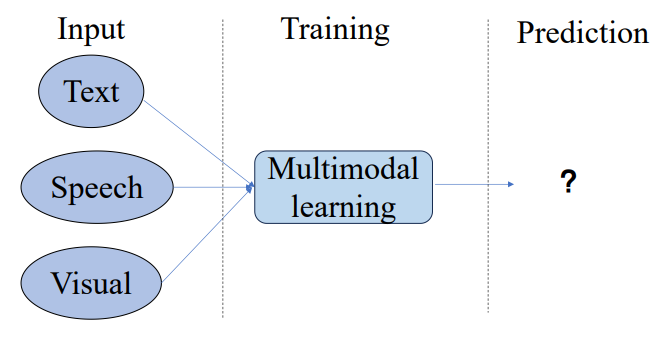
\includegraphics[width=0.8\textwidth]{bab2/multimodal.png}
\caption[Visualisasi definisi \textit{multimodal}]{Visualisasi definisi \textit{multimodal} \parencite{10386743}}
\label{fig:multimodal_definition}
\end{figure} 

Menurut \textcite{wuMultimodalLargeLanguage2023}, pengembangan teknis model \textit{multimodal} mencakup lima aspek fundamental, yaitu representasi pengetahuan, pemilihan tujuan pembelajaran, konstruksi struktur model, fusi informasi, dan penggunaan \textit{prompts}. Kelima aspek yang diilustrasikan pada Gambar \ref{fig:multimodal_model_points} ini dijabarkan sebagai berikut. Representasi pengetahuan dimulai dengan proses tokenisasi dan \textit{embedding} untuk mengubah data teks dan citra menjadi format vektor yang dapat diproses. Untuk teks, metode seperti \textit{byte pair encoding} umum digunakan, sedangkan citra diproses melalui pendekatan berbasis \textit{region}, \textit{grid}, atau \textit{patch} yang membagi gambar menjadi bagian-bagian kecil. Setelah data terwakili, pemilihan tujuan pembelajaran menjadi krusial untuk melatih model memahami hubungan antar \textit{modality}. Teknik seperti \textit{Image-Text Contrast} (ITC) digunakan untuk menyelaraskan representasi citra dan teks, sementara \textit{Masked Language Modeling} (MLM) dan \textit{Masked Visual Modeling} (MVM) melatih model merekonstruksi informasi yang hilang untuk memahami konteks secara mendalam.

\begin{figure}[H]
\centering
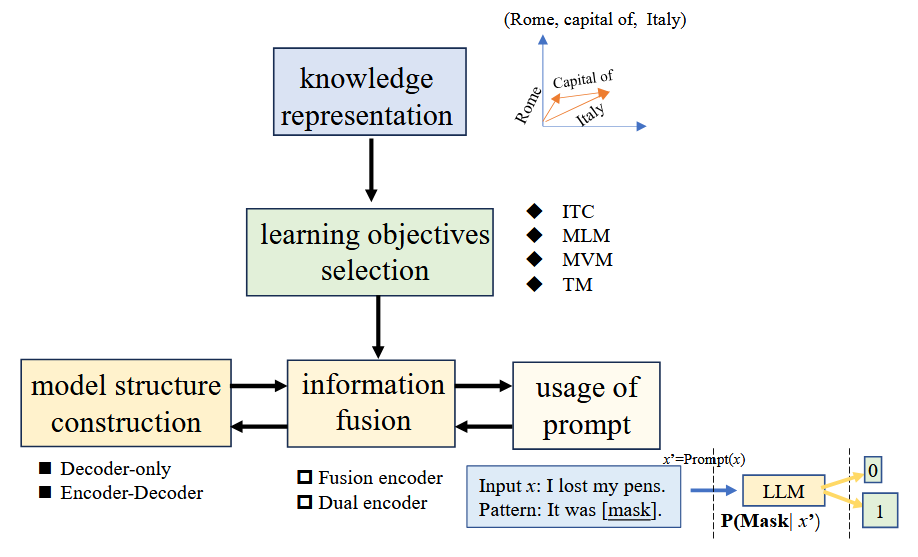
\includegraphics[width=0.8\textwidth]{bab2/multimodalmodelpoints.png}
\caption[Aspek utama dalam model \textit{multimodal}]{Aspek utama dalam model \textit{multimodal} \parencite{wuMultimodalLargeLanguage2023}}
\label{fig:multimodal_model_points}
\end{figure}

Konstruksi struktur model \textit{multimodal} umumnya dikategorikan menjadi arsitektur \textit{encoder-only} dan \textit{encoder-decoder}. Arsitektur \textit{encoder-only} memproses masukan secara langsung melalui \textit{encoder} dan lebih cocok untuk tugas pencarian (\textit{retrieval}), sedangkan arsitektur \textit{encoder-decoder} memanfaatkan kemampuan \textit{decoder} untuk membangkitkan luaran secara autoregresif sehingga ideal untuk tugas generatif. Fusi informasi (\textit{information fusion}) berfokus pada mekanisme penggabungan fitur multimodal, baik melalui fusi awal (\textit{early fusion}) maupun fusi akhir (\textit{late fusion}), untuk menghasilkan pemahaman yang komprehensif. Dalam konteks ini, terdapat pendekatan \textit{fusion encoder} dan \textit{dual encoder}. \textit{Fusion encoder} memungkinkan interaksi mendalam antar \textit{modality} melalui mekanisme \textit{attention} yang memberikan hasil inferensi yang kuat namun dengan biaya komputasi yang lebih tinggi. Sebaliknya, \textit{dual encoder} memproses setiap \textit{modality} secara terpisah sebelum menghitung kesamaan menggunakan operasi sederhana, menjadikannya lebih efisien untuk tugas pencarian data.

Penggunaan \textit{prompt} memainkan peran penting dalam menjembatani kesenjangan antara fase pra-pelatihan dan aplikasi pada tugas hilir. Dengan memodifikasi format tugas melalui instruksi tekstual, \textit{prompt} membantu model beradaptasi dengan tugas baru tanpa memerlukan pembaruan parameter yang ekstensif, sehingga mengurangi biaya \textit{fine-tuning}. Pendekatan ini memungkinkan model menangani skenario dengan sedikit atau tanpa contoh data. Dalam praktiknya, penggunaan \textit{prompt} yang informatif dapat meningkatkan pemahaman model terhadap konteks visual dan tekstual, serta memfasilitasi interaksi yang lebih alami antara pengguna dan sistem \textit{multimodal}. 

\textcite{huyenAIEngineeringBuilding2025} mengemukakan bahwa perkembangan pesat model \textit{multimodal} saat ini berjalan seiring dengan kesuksesan arsitektur \textit{Large Language Models} (LLM) berbasis \textit{Transformer} yang telah berevolusi menjadi \textit{foundation models}. Model-model generatif ini menjalani pelatihan ekstensif menggunakan himpunan data yang luas dan beragam, yang memungkinkannya untuk menangkap pola umum dan hubungan dalam data yang tidak hanya terbatas pada teks, tetapi juga mencakup format data lain seperti citra, audio, dan video \parencite{altoBuildingLLMPowerd2024}. \textcite{huyenAIEngineeringBuilding2025} merujuk pada model \textit{multimodal} generatif ini sebagai \textit{Large Multimodal Models} (LMM), sementara \textcite{altoBuildingLLMPowerd2024} menggunakan istilah \textit{Large Foundation Models} (LFM), dan \textcite{yinSurveyMultimodalLarge2024} menyebutnya sebagai \textit{Multimodal Large Language Models} (MLLM). Walaupun menggunakan terminologi yang berbeda, ketiga istilah tersebut pada dasarnya mengacu pada konsep yang sama. Kemampuan model-model ini dalam mengintegrasikan berbagai \textit{modality} data menjadi fondasi penting bagi pengembangan sistem kecerdasan buatan yang lebih adaptif dan mampu memahami kompleksitas dunia nyata secara holistik.

\subsection{\textit{Multimodal Large Language Models} (MLLM)}
\textcite{yinSurveyMultimodalLarge2024} mendefinisikan MLLM secara formal sebagai model berbasis LLM yang memiliki kemampuan untuk menerima, melakukan penalaran, dan menghasilkan luaran dengan informasi \textit{multimodal}. Arsitektur tipikal MLLM terdiri dari \textit{encoder}, konektor, dan LLM. Sebuah generator opsional dapat ditambahkan pada LLM untuk menghasilkan \textit{modality} lain selain teks. \textit{Encoder} berfungsi menerima masukan berupa citra, audio, atau video dan menghasilkan fitur, yang kemudian diproses oleh konektor agar dapat dipahami oleh LLM. Ilustrasi arsitektur ini disajikan pada Gambar \ref{fig:mllm_architecture}.

\begin{figure}[H]
\centering
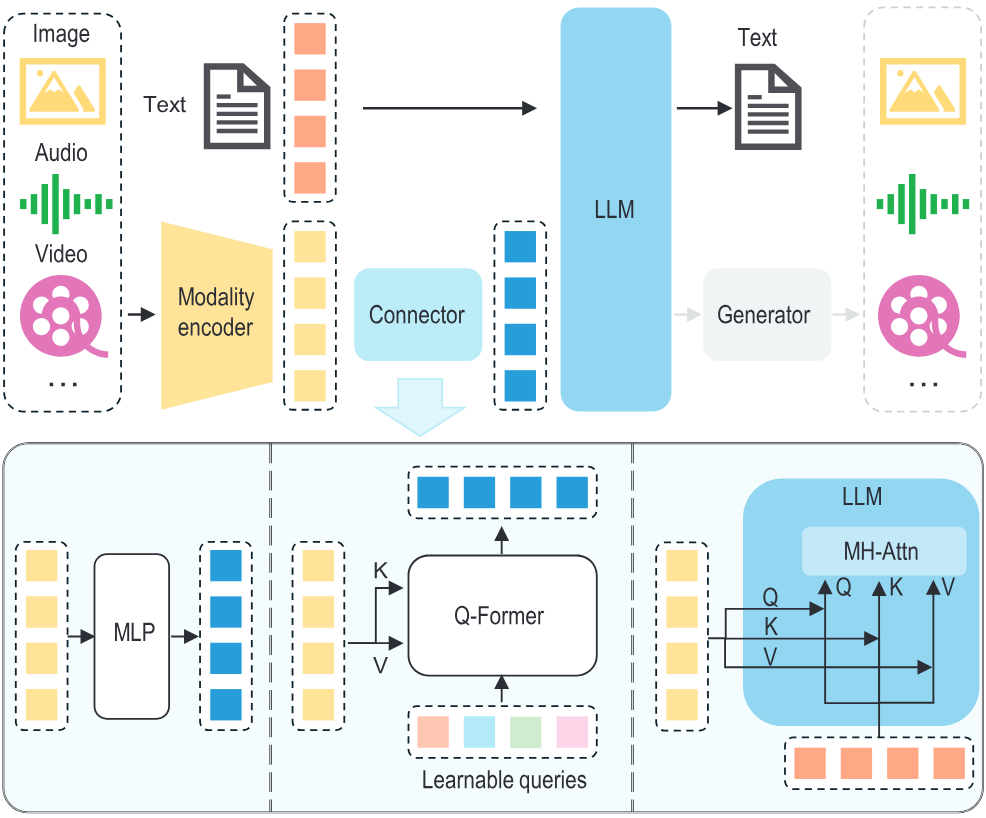
\includegraphics[width=\textwidth]{bab2/mllm.png}
\caption[Ilustrasi arsitektur tipikal MLLM]{Ilustrasi arsitektur tipikal MLLM yang mencakup \textit{encoder}, konektor, dan LLM \parencite{yinSurveyMultimodalLarge2024}}
\label{fig:mllm_architecture}
\end{figure}

Secara umum, pengembangan MLLM dapat diabstraksikan menjadi tiga modul utama, yaitu \textit{modality encoder} yang telah dilatih sebelumnya (\textit{pre-trained}), LLM yang telah dilatih sebelumnya, dan antarmuka \textit{modality} (\textit{modality interface}) untuk menghubungkan keduanya. \textcite{yinSurveyMultimodalLarge2024} menganalogikan struktur ini dengan manusia, di mana \textit{modality encoder} (seperti \textit{encoder} citra atau audio) berperan sebagai mata atau telinga yang menerima dan memproses sinyal optik atau akustik, sedangkan LLM bertindak layaknya otak yang memahami dan melakukan penalaran terhadap sinyal yang telah diproses tersebut.

Modul pertama, \textit{modality encoder}, bertugas mengompresi informasi mentah seperti citra atau audio menjadi representasi yang lebih ringkas \parencite{yinSurveyMultimodalLarge2024}. Penggunaan \textit{encoder} yang telah dilatih sebelumnya dan diselaraskan dengan \textit{modality} lain lebih umum dilakukan daripada melatih model dari awal. Sebagai contoh, CLIP \parencite{radfordLearningTransferableVisual2021} menggunakan \textit{visual encoder} yang secara semantik telah diselaraskan dengan teks melalui pra-pelatihan skala besar. Penggunaan \textit{encoder} semacam ini memudahkan proses penyelarasan dengan LLM. Modul kedua adalah LLM pra-latih. Memulai pengembangan dengan LLM yang telah dilatih sebelumnya dinilai lebih efisien dan praktis. Melalui pelatihan ekstensif pada korpus teks yang masif, LLM telah dilengkapi dengan pengetahuan dunia yang kaya serta kemampuan generalisasi dan penalaran yang kuat.

Modul ketiga adalah antarmuka \textit{modality} \parencite{yinSurveyMultimodalLarge2024}. Mengingat LLM hanya memproses teks dan tingginya biaya komputasi pelatihan \textit{end-to-end}, diperlukan jembatan untuk menghubungkan kesenjangan antara bahasa alami dan \textit{modality} lainnya. Oleh karena itu, pendekatan yang lebih praktis adalah dengan memperkenalkan konektor yang dapat dilatih (\textit{learnable connector}) di antara \textit{visual encoder} dan LLM. Dalam pendekatan menggunakan konektor, komponen ini berfungsi untuk menyelaraskan representasi dari \textit{modality} yang berbeda agar dapat diproses oleh LLM. Terdapat tiga jenis konektor utama, yaitu berbasis proyeksi, berbasis \textit{query}, dan berbasis fusi. Dua jenis pertama mengadopsi fusi tingkat token yang memproses fitur menjadi token untuk dikirim bersama token teks, sedangkan jenis terakhir memungkinkan fusi tingkat fitur di dalam LLM. Sebagai alternatif, pendekatan lain memanfaatkan model ahli (\textit{expert models}) seperti \textit{image captioning} untuk mengonversi masukan \textit{multimodal} menjadi teks, sehingga dapat diproses langsung oleh LLM tanpa pelatihan tambahan. Meskipun pendekatan ini lebih sederhana, penggunaannya tidak sefleksibel antarmuka yang dapat dilatih karena konversi modalitas asing ke dalam bentuk teks berpotensi menyebabkan hilangnya informasi.

\subsection{\textit{Vision-Language Models} (VLM)}
\textit{Vision-Language Models} (VLM) adalah kelas model kecerdasan buatan \textit{multimodal} yang dirancang untuk memproses dan menghubungkan informasi dari \textit{modality} visual (citra atau video) dan tekstual (bahasa alami) secara bersamaan. Tujuan utama dari VLM adalah untuk menjembatani kesenjangan semantik antara representasi visual dan linguistik, sehingga memungkinkan mesin untuk "melihat" dan "memahami" dunia visual serta mengomunikasikannya melalui bahasa manusia \parencite{bordesIntroductionVisionLanguageModeling2024}. Kemampuan ini menjadi fondasi bagi berbagai aplikasi cerdas, mulai dari pencarian gambar berbasis teks, deskripsi gambar otomatis, hingga sistem tanya jawab visual yang kompleks.

Berdasarkan strategi pelatihan dan arsitekturnya, \textcite{bordesIntroductionVisionLanguageModeling2024} mengklasifikasikan VLM ke dalam empat keluarga utama yang menggambarkan evolusi integrasi \textit{modality} visual dan tekstual, sebagaimana disajikan pada Gambar \ref{fig:vlm_families}. Kategori pertama adalah \textit{contrastive learning} yang berfokus pada penyelarasan ruang representasi antara citra dan teks menggunakan fungsi kerugian kontras untuk mendekatkan representasi pasangan data yang cocok. Kategori kedua, \textit{masking}, menerapkan mekanisme rekonstruksi bagian input yang ditutupi untuk mempelajari hubungan kontekstual antara elemen visual dan tekstual. Selanjutnya, kategori \textit{generative} mencakup model yang dilatih dengan tujuan utama membangkitkan data secara autoregresif, baik berupa teks dari citra maupun sebaliknya. Terakhir, kategori \textit{pretrained backbones} memanfaatkan model bahasa dan \textit{vision encoder} yang telah dilatih sebelumnya sebagai komponen dasar yang dibekukan, di mana pelatihan hanya difokuskan pada modul penghubung untuk memetakan fitur visual ke dalam ruang input model bahasa.

\begin{figure}[H]
\centering
\includegraphics[width=0.7\textwidth]{bab2/vlmfamilies.png}
\caption[Empat Kategori Utama \textit{Vision-Language Models}]{Empat Kategori Utama \textit{Vision-Language Models}: (1) \textit{Contrastive}, (2) \textit{Masking}, (3) \textit{Generative}, dan (4) \textit{Pretrained Backbones} \parencite{bordesIntroductionVisionLanguageModeling2024}}
\label{fig:vlm_families}
\end{figure}

Evaluasi kinerja VLM dilakukan menggunakan berbagai metrik dan tugas standar untuk mengukur kemampuan visio-linguistiknya secara komprehensif. Taksonomi evaluasi VLM sebagaimana dijelaskan oleh \textcite{bordesIntroductionVisionLanguageModeling2024} divisualisasikan pada Gambar \ref{fig:vlm_evaluation}. Salah satu tugas evaluasi yang paling fundamental adalah \textit{Visual Question Answering} (VQA). Dalam VQA, model diberikan sebuah citra dan pertanyaan bahasa alami terkait citra tersebut, kemudian diminta untuk menghasilkan jawaban yang akurat. Tugas ini menuntut kemampuan penalaran tingkat tinggi karena model tidak hanya harus mengenali objek dalam citra, tetapi juga memahami hubungan spasial, aktivitas, dan konteks semantik yang ditanyakan \parencite{bordesIntroductionVisionLanguageModeling2024}. VQA dianggap sebagai proksi yang kuat untuk mengukur pemahaman \textit{multimodal} yang mendalam. Selain VQA, evaluasi juga mencakup kemampuan \textit{zero-shot classification}, penalaran komposisional (\textit{compositional reasoning}) untuk mendeteksi nuansa linguistik yang halus, serta pengujian terhadap halusinasi objek untuk memastikan reliabilitas model dalam aplikasi dunia nyata.

\begin{figure}[H]
\centering
\includegraphics[width=0.8\textwidth]{bab2/vlmevaluation.png}
\caption[Taksonomi Evaluasi \textit{Vision-Language Models}]{Taksonomi Evaluasi \textit{Vision-Language Models} \parencite{bordesIntroductionVisionLanguageModeling2024}}
\label{fig:vlm_evaluation}
\end{figure}

\subsection{\textit{Contrastive Language-Image Pre-training} (CLIP)}
\textit{Contrastive Language-Image Pre-training} (CLIP) merupakan model \textit{multimodal} yang diperkenalkan oleh \textcite{radfordLearningTransferableVisual2021} untuk menjembatani kesenjangan antara \textit{computer vision} dan pemahaman bahasa alami. Berbeda dengan pendekatan visi komputer konvensional yang bergantung pada \textit{dataset} dengan label kelas yang kaku dan terbatas, CLIP dilatih menggunakan pengawasan alami (\textit{natural language supervision}) dari pasangan citra dan teks yang tersedia secara melimpah di internet. Pendekatan ini memungkinkan model untuk mempelajari representasi visual yang kaya dan fleksibel, serta memiliki kemampuan \textit{zero-shot transfer} yang memungkinkannya mengenali kategori objek baru tanpa perlu dilatih ulang secara spesifik.

\textcite{radfordLearningTransferableVisual2021} merancang arsitektur CLIP dengan dua komponen utama, yaitu \textit{Image Encoder} dan \textit{Text Encoder}. \textit{Image Encoder} bertugas untuk memproses data visual menjadi vektor fitur, yang dapat menggunakan arsitektur ResNet atau \textit{Vision Transformer} (ViT). Sementara itu, \textit{Text Encoder} menggunakan arsitektur \textit{Transformer} untuk mengubah deskripsi teks menjadi vektor fitur dalam ruang dimensi yang sama. Mekanisme pelatihan CLIP didasarkan pada pembelajaran kontras (\textit{contrastive learning}), di mana model dilatih untuk memprediksi pasangan citra dan teks yang benar dari sekumpulan kemungkinan pasangan acak dalam sebuah \textit{batch}. Secara matematis, CLIP memaksimalkan kesamaan kosinus (\textit{cosine similarity}) antara \textit{embedding} citra dan teks yang berpasangan ($N$ pasangan asli) sambil meminimalkan kesamaan antara pasangan yang tidak cocok ($N^2 - N$ pasangan salah). Arsitektur dan mekanisme pelatihan CLIP diilustrasikan pada Gambar \ref{fig:clip_architecture}.

\begin{figure}[H]
\centering
\includegraphics[width=\textwidth]{bab2/arsitekturclip.png}
\caption[Arsitektur dan mekanisme pelatihan CLIP]{Arsitektur dan mekanisme pelatihan CLIP \parencite{radfordLearningTransferableVisual2021}}
\label{fig:clip_architecture}
\end{figure}

Keunggulan CLIP dalam mempelajari representasi visual yang kuat telah menginspirasi pengembangan model turunan untuk domain spesifik, salah satunya adalah SCOLD (\textit{Soft-target COntrastive learning for Leaf Disease identification}) yang diusulkan oleh \textcite{quocVisionLanguageFoundationModel2025}. SCOLD merupakan \textit{Vision-Language Foundation Model} yang secara khusus dikembangkan untuk pengenalan penyakit tanaman. Model ini mengadaptasi arsitektur CLIP dan menyempurnakannya melalui teknik \textit{fine-tuning} serta penerapan \textit{Deep Metric Learning}.

Dalam pengembangannya, \textcite{quocVisionLanguageFoundationModel2025} merancang SCOLD untuk mengatasi tantangan variabilitas visual yang tinggi pada gejala penyakit tanaman yang sering kali sulit dibedakan oleh model umum. Arsitektur SCOLD mempertahankan struktur \textit{encoder} ganda dari CLIP, namun dioptimalkan untuk memetakan fitur penyakit tanaman ke dalam ruang representasi yang lebih diskriminatif. Hal ini dicapai dengan melatih model agar jarak antara representasi citra penyakit dan deskripsi teksnya menjadi lebih dekat, sementara jarak dengan kelas penyakit lain diperlebar. Visualisasi arsitektur SCOLD dapat dilihat pada Gambar \ref{fig:scold_architecture}.

\begin{figure}[H]
\centering
\includegraphics[width=\textwidth]{bab2/arsitekturscold.png}
\caption[Arsitektur SCOLD]{Arsitektur SCOLD untuk pengenalan penyakit tanaman \parencite{quocVisionLanguageFoundationModel2025}}
\label{fig:scold_architecture}
\end{figure}

Efektivitas SCOLD dibandingkan dengan model CLIP standar dievaluasi oleh \textcite{quocVisionLanguageFoundationModel2025} menggunakan \textit{dataset} LeafNet, yang dibuat secara khusus untuk mengembangkan SCOLD, melalui tugas pengambilan lintas \textit{modal} (\textit{cross-modal retrieval}), yaitu \textit{Image-to-Text Retrieval} dan \textit{Text-to-Image Retrieval}. Hasil evaluasi menunjukkan bahwa SCOLD secara konsisten mengungguli CLIP pada metrik Recall@K (R@1, R@5, dan R@10) untuk kedua tugas tersebut. Peningkatan performa ini mengindikasikan bahwa proses \textit{fine-tuning} dan adaptasi domain yang dilakukan pada SCOLD berhasil meningkatkan keselarasan semantik antara fitur visual gejala penyakit dan deskripsi tekstualnya. Perbandingan kinerja pengambilan informasi antara CLIP dan SCOLD disajikan pada Tabel \ref{tab:scold_performance}.

\begin{table}[H]
    \centering
    \caption[Perbandingan performa retrieval SCOLD dan CLIP]
    {Perbandingan \textit{retrieval} SCOLD dan CLIP pada \textit{dataset} LeafNet \parencite{quocVisionLanguageFoundationModel2025}}
    \label{tab:scold_performance}
    \setstretch{1.0}
    \begin{tblr}{
        width = \linewidth,
        colspec = {X[l, m] *{6}{X[c, m]}},
        hlines, vlines,
        rows = {m},
        rowsep = 4pt,
        row{1,2} = {font=\bfseries, halign=c, valign=m},
        cell{1}{1} = {r=2}{},
        cell{1}{2} = {c=3}{},
        cell{1}{5} = {c=3}{},
    }
    Metode & \textit{Image-to-Text} & & & \textit{Text-to-Image} & & \\
    & R@1 (\%) & R@5 (\%) & R@10 (\%) & R@1 (\%) & R@5 (\%) & R@10 (\%) \\
    CLIP & 95.01 & 97.89 & 99.85 & 95.31 & 98.18 & 99.89 \\
    SCOLD
        & \textbf{95.49} {\footnotesize(+0.48)}
        & \textbf{98.85} {\footnotesize(+0.96)}
        & \textbf{99.93} {\footnotesize(+0.08)}
        & \textbf{95.46} {\footnotesize(+0.15)}
        & \textbf{99.70} {\footnotesize(+1.52)}
        & \textbf{99.99} {\footnotesize(+0.10)} \\
    \end{tblr}
\end{table}


% Efektivitas SCOLD dibandingkan dengan model CLIP standar dievaluasi oleh \textcite{quocVisionLanguageFoundationModel2025} menggunakan \textit{dataset} LeafNet, yang dibuat secara khusus untuk mengembangkan SCOLD, melalui tugas pengambilan lintas \textit{modal} (\textit{cross-modal retrieval}), yaitu \textit{Image-to-Text Retrieval} dan \textit{Text-to-Image Retrieval}. Hasil evaluasi menunjukkan bahwa SCOLD secara konsisten mengungguli CLIP pada metrik \textit{Recall@K} (R@1, R@5, dan R@10). Pada tugas \textit{Image-to-Text Retrieval}, SCOLD mencatatkan akurasi R@1 sebesar 95,49\%, R@5 sebesar 98,85\%, dan R@10 sebesar 99,93\%, unggul dibandingkan CLIP yang masing-masing memperoleh 95,01\%, 97,89\%, dan 99,85\%. Tren serupa terlihat pada \textit{Text-to-Image Retrieval}, di mana SCOLD mencapai R@1 sebesar 95,46\%, R@5 sebesar 99,7\%, dan R@10 sebesar 99,99\%, melampaui CLIP yang mencatatkan 95,31\%, 98,18\%, dan 99,89\%. Peningkatan performa ini mengindikasikan bahwa proses \textit{fine-tuning} dan adaptasi domain yang dilakukan pada SCOLD berhasil meningkatkan keselarasan semantik antara fitur visual gejala penyakit dan deskripsi tekstualnya \parencite{quocVisionLanguageFoundationModel2025}.

\subsection{Keluarga Model Gemini}
Gemini merupakan keluarga model \textit{multimodal} yang dikembangkan oleh Google DeepMind \parencite{teamGeminiFamilyHighly2025}. Berbeda dengan pendekatan konvensional yang melatih komponen secara terpisah untuk \textit{modality} yang berbeda, Gemini dibangun secara natif (\textit{natively multimodal}). Model ini dilatih sejak awal pada sekumpulan data \textit{multimodal} yang mencakup teks, kode, gambar, audio, dan video secara bersamaan. Pendekatan ini memungkinkan model untuk memiliki pemahaman dan penalaran lintas \textit{modality} yang kuat serta kemampuan untuk menerima masukan dan menghasilkan luaran dalam berbagai format secara mulus \parencite{teamGeminiFamilyHighly2025}. Gambaran umum mengenai kemampuan \textit{multimodal} model ini diilustrasikan pada Gambar \ref{fig:gemini_overview}.

\begin{figure}[H]
\centering
\includegraphics[width=0.8\textwidth]{bab2/geminimodeloverview.png}
\caption[Gambaran umum kemampuan \textit{multimodal} Gemini]{Gambaran umum kemampuan \textit{multimodal} Gemini \parencite{teamGeminiFamilyHighly2025}}
\label{fig:gemini_overview}
\end{figure}

Evolusi keluarga model ini dimulai dengan Gemini 1.0 yang memperkenalkan tiga varian utama, yaitu Ultra, Pro, dan Nano, masing-masing dioptimalkan untuk tingkat kompleksitas tugas dan efisiensi sumber daya yang berbeda. Pengembangan model ini dilanjutkan dengan diperkenalkannya Gemini 1.5 \parencite{teamGemini15Unlocking2024}. Inovasi utama pada Gemini 1.5 adalah perluasan jendela konteks hingga jutaan token, yang memfasilitasi pemrosesan dokumen panjang atau basis kode yang besar dalam satu kali interaksi.

Evolusi selanjutnya hadir melalui keluarga Gemini 2.5, yang difokuskan pada peningkatan kemampuan penalaran lanjut dan menyeimbangkan performa tinggi dengan efisiensi operasional \parencite{comaniciGemini25Pushing2025}. Gemini 2.5 dibangun menggunakan arsitektur \textit{Mixture-of-Experts}, di mana model hanya mengaktifkan subset parameter yang relevan untuk setiap input, sehingga meningkatkan efisiensi inferensi tanpa mengorbankan kualitas luaran. Model ini juga dilatih menggunakan teknik \textit{Chain-of-Thought}, yang memberikannya kemampuan penalaran dalam menyelesaikan masalah logika kompleks, matematika, dan pemrograman. Gemini 2.5 dirancang untuk menangani instruksi yang kompleks serta mempertahankan koherensi dalam tugas-tugas yang membutuhkan perencanaan bertahap. Seri model ini mencakup varian Gemini 2.5 Pro yang dioptimalkan untuk performa penalaran tertinggi, serta Gemini 2.5 Flash yang dirancang untuk efisiensi dan latensi rendah. Kemampuan varian Pro dalam berbagai \textit{benchmark} diperlihatkan pada Tabel \ref{tab:gemini25_pro_benchmark}.

{
\setstretch{1.0}
\begin{longtblr}[
    caption = {Hasil \textit{benchmark} Gemini 2.5 Pro pada berbagai tugas \parencite{comaniciGemini25Pushing2025}},
    entry = {Hasil \textit{benchmark} Gemini 2.5 Pro pada berbagai tugas},
    label = {tab:gemini25_pro_benchmark},
]{
    width = \linewidth,
    colspec = {X[1.4,l] X[1.7,l] *{4}{X[c]}},
    rows = {m},
    rowhead = 1,
    row{1} = {font=\bfseries, halign=c, valign=m},
    row{16} = {font=\bfseries, halign=c, valign=m},
    hlines, vlines,
    rowsep = 3pt,
}
    % ---- BLOK 1: Header ----
    \textit{Capability} & \textit{Benchmark} & {Gemini 2.5\\Pro} & {o3\\high} & {o4-mini\\high} & {Claude 4\\Sonnet} \\
    % ---- Code ----
    \textit{Code} & LiveCodeBench & 74.2\% & 72.0\% & \textbf{75.8\%} & 48.9\% \\
    \textit{Code} & Aider Polyglot & \textbf{82.2\%} & 79.6\% & 72.0\% & 61.3\% \\
    \textit{Code} & SWE-bench Verified \textit{(single)} & 59.6\% & 69.1\% & 68.1\% & \textbf{72.7\%} \\
    \textit{Code} & SWE-bench Verified \textit{(multiple)} & 67.2\% & -- & -- & \textbf{80.2\%} \\
    % ---- Reasoning ----
    \textit{Reasoning} & GPQA (diamond) \textit{(single)} & \textbf{86.4\%} & 83.3\% & 81.4\% & 75.4\% \\
    \textit{Reasoning} & Humanity's Last Exam \textit{(no tools)} & \textbf{21.6\%} & 20.3\% & 18.1\% & 7.8\% \\
    % ---- Factuality ----
    \textit{Factuality} & SimpleQA & \textbf{54.0\%} & 48.6\% & 19.3\% & -- \\
    \textit{Factuality} & FACTS Grounding & \textbf{87.8\%} & 69.9\% & 62.1\% & 79.1\% \\
    % ---- Math ----
    \textit{Math} & AIME 2025 \textit{(single)} & 88.0\% & 88.9\% & \textbf{92.7\%} & 70.5\% \\
    % ---- Long-context ----
    \textit{Long-context} & LOFT (hard retrieval) $\le$128K & \textbf{87.0\%} & 77.0\% & 60.5\% & 81.6\% \\
    \textit{Long-context} & LOFT (hard retrieval) 1M & \textbf{69.8\%} & -- & -- & -- \\
    \textit{Long-context} & MRCR-V2 (8-needle) $\le$128K & \textbf{58.0\%} & 57.1\% & 36.3\% & 39.1\% \\
    \textit{Long-context} & MRCR-V2 (8-needle) 1M & \textbf{16.4\%} & -- & -- & -- \\
    % ---- Image ----
    \textit{Image Und.} & MMMU \textit{(single)} & 82.0\% & \textbf{82.9\%} & 81.6\% & 74.4\% \\
    % ---- BLOK 2: Header ulang ----
    \textit{Capability} & \textit{Benchmark} & {Claude 4\\Opus} & {Grok 3 Beta\\Ext. Thinking} & \SetCell[c=2]{c} {DeepSeek R1\\0528} \\
    % ---- Code ----
    \textit{Code} & LiveCodeBench & 51.1\% & -- & \SetCell[c=2]{c} 70.5\% \\
    \textit{Code} & Aider Polyglot & 72.0\% & 53.3\% & \SetCell[c=2]{c} 71.6\% \\
    \textit{Code} & SWE-bench Verified \textit{(single)} & 72.5\% & -- & \SetCell[c=2]{c} -- \\
    \textit{Code} & SWE-bench Verified \textit{(multiple)} & 79.4\% & -- & \SetCell[c=2]{c} 57.6\% \\
    % ---- Reasoning ----
    \textit{Reasoning} & GPQA (diamond) \textit{(single)} & 79.6\% & 80.2\% & \SetCell[c=2]{c} 81.0\% \\
    \textit{Reasoning} & Humanity's Last Exam \textit{(no tools)} & 10.7\% & -- & \SetCell[c=2]{c} 14.0\% \\
    % ---- Factuality ----
    \textit{Factuality} & SimpleQA & -- & 43.6\% & \SetCell[c=2]{c} 27.8\% \\
    \textit{Factuality} & FACTS Grounding & 77.7\% & 74.8\% & \SetCell[c=2]{c} 82.4\% \\
    % ---- Math ----
    \textit{Math} & AIME 2025 \textit{(single)} & 75.5\% & 77.3\% & \SetCell[c=2]{c} 87.5\% \\
    % ---- Long-context ----
    \textit{Long-context} & LOFT (hard retrieval) $\le$128K & -- & 73.1\% & \SetCell[c=2]{c} -- \\
    \textit{Long-context} & LOFT (hard retrieval) 1M & -- & -- & \SetCell[c=2]{c} -- \\
    \textit{Long-context} & MRCR-V2 (8-needle) $\le$128K & 16.1\% & 34.0\% & \SetCell[c=2]{c} -- \\
    \textit{Long-context} & MRCR-V2 (8-needle) 1M & -- & -- & \SetCell[c=2]{c} -- \\
    % ---- Image ----
    \textit{Image Und.} & MMMU \textit{(single)} & 76.5\% & 76.0\% & \SetCell[c=2]{c} \textit{No MM} \\
\end{longtblr}
}

Selain varian Pro, \textcite{comaniciGemini25Pushing2025} menyoroti kemampuan Gemini 2.5 Flash yang menawarkan keunggulan dalam kecepatan pemrosesan. Karakteristik ini menjadikannya solusi yang sesuai untuk aplikasi yang membutuhkan respons instan atau pemrosesan volume data yang besar. Perbandingan kecepatan inferensi yang signifikan pada varian Flash ditunjukkan pada Gambar \ref{fig:gemini25_flash_speed}.

\begin{figure}[H]
\centering
\includegraphics[width=0.8\textwidth]{bab2/gemini2.5flashisfast.png}
\caption[Perbandingan kecepatan Gemini 2.5 Flash]{Perbandingan kecepatan Gemini 2.5 Flash \parencite{comaniciGemini25Pushing2025}}
\label{fig:gemini25_flash_speed}
\end{figure}

Selain keunggulan dalam kecepatan, \textcite{comaniciGemini25Pushing2025} juga mencatat bahwa Gemini 2.5 menunjukkan peningkatan performa yang signifikan. Peningkatan ini terlihat jelas jika dibandingkan dengan model-model pendahulunya. Perbandingan kemampuan model-model dalam keluarga Gemini hingga versi 2.5 diperlihatkan pada Tabel \ref{tab:gemini25_comparisons}.

{
\setstretch{1.0}
\begin{longtblr}[
    caption = {Perbandingan kemampuan keluarga model Gemini hingga versi 2.5 \parencite{comaniciGemini25Pushing2025}},
    entry = {Perbandingan kemampuan keluarga model Gemini},
    label = {tab:gemini25_comparisons},
]{
        width = \linewidth,
        colspec = {X[1.1,l] *{6}{X[c]}},
        hlines, vlines,
        rows = {m},
        rowsep = 4pt,
        row{1} = {font=\bfseries, halign=c, valign=m},
        column{1} = {font=\bfseries},
        rowhead = 1,
    }
    Fitur & {Gemini 1.5\\Flash} & {Gemini 1.5\\Pro} & {Gemini 2.0\\Flash-Lite} & {Gemini 2.0\\Flash} & {Gemini 2.5\\Flash} & {Gemini 2.5\\Pro} \\
    \textit{Modality} masukan & Teks, Citra, Video, Audio & Teks, Citra, Video, Audio & Teks, Citra, Video, Audio & Teks, Citra, Video, Audio & Teks, Citra, Video, Audio & Teks, Citra, Video, Audio \\
    Panjang masukan & 1M & 2M & 1M & 1M & 1M & 1M \\
    \textit{Modality} luaran & Teks & Teks & Teks & Teks, Citra* & Teks, Audio* & Teks, Audio* \\
    Panjang luaran & 8K & 8K & 8K & 8K & 64K & 64K \\
    \textit{Thinking} & Tidak & Tidak & Tidak & Ya* & Dinamis & Dinamis \\
    {Dukung\newline an} \textit{tool} & Tidak & Tidak & Tidak & Ya & Ya & Ya \\
    {Batas pengetahu\newline an} & November 2023 & November 2023 & Juni 2024 & Juni 2024 & Januari 2025 & Januari 2025 \\
\end{longtblr}
}

Iterasi terbaru yang saat ini diperkenalkan adalah seri Gemini 3, yang kembali menghadirkan varian Pro dan Flash dengan peningkatan pada arsitektur dasarnya. Gemini 3 Pro dirancang sebagai model dengan kemampuan penalaran terbaik di kelasnya, mampu menangani nuansa bahasa dan logika yang paling kompleks \parencite{google2025}. Peningkatan ini memungkinkan model untuk memproses instruksi yang rumit dengan akurasi yang lebih tinggi, khususnya pada domain yang memerlukan pemahaman konteks yang mendalam. Di sisi lain, Gemini 3 Flash menargetkan keseimbangan optimal antara kecerdasan, kecepatan, dan biaya operasional, serta kemampuan agentik yang lebih andal untuk eksekusi tugas otomatis \parencite{googleGemini3Flash2025}. Dengan latensi yang lebih rendah, varian Flash ini dioptimalkan untuk skenario penggunaan skala besar yang menuntut efisiensi waktu dan sumber daya komputasi. Performa kedua model ini dalam berbagai pengujian standar dapat dilihat pada Tabel \ref{tab:gemini3_pro_benchmark}.

{
\setstretch{1.0}
\begin{longtblr}[
    caption = {Hasil \textit{benchmark} Gemini 3 Pro pada berbagai tugas \parencite{google2025}},
    label = {tab:gemini3_pro_benchmark},
    entry = {Hasil \textit{benchmark} Gemini 3 Pro},
]{
    width = \linewidth,
    colspec = {X[2,l] X[1.5,l] *{4}{X[1,c]}},
    rows = {m},
    rowhead = 1,
    row{1} = {font=\bfseries, halign=c, valign=m},
    hlines, vlines,
    rowsep = 3pt,
}
    \textit{Benchmark} & Deskripsi & {Gemini 3\\Pro} & {Gemini 2.5\\Pro} & {Claude 4.5\\Sonnet} & {GPT-5.1} \\
    Humanity's Last Exam & \textit{Academic reasoning} & {\textbf{37.5\%} \scriptsize (no tools) \\ \textbf{45.8\%} \scriptsize (code)} & 21.6\% & 13.7\% & 26.5\% \\
    ARC-AGI-2 & \textit{Visual reasoning puzzles} & \textbf{31.1\%} & 4.9\% & 13.6\% & 17.6\% \\
    GPQA Diamond & \textit{Scientific knowledge} & \textbf{91.9\%} & 86.4\% & 83.4\% & 88.1\% \\
    AIME 2025 & \textit{Mathematics} & {95.0\% \scriptsize (no tools) \\ \textbf{100\%} \scriptsize (code)} & 88.0\% & {87.0\% \\ \textbf{100\%}} & 94.0\% \\
    MathArena Apex & \textit{Math Contest problems} & \textbf{23.4\%} & 0.5\% & 1.6\% & 1.0\% \\
    MMMU-Pro & \textit{Multimodal reasoning} & \textbf{81.0\%} & 68.0\% & 68.0\% & 76.0\% \\
    ScreenSpot-Pro & \textit{Screen understanding} & \textbf{72.7\%} & 11.4\% & 36.2\% & 3.5\% \\
    CharXiv Reasoning & \textit{Chart information synthesis} & \textbf{81.4\%} & 69.6\% & 68.5\% & 69.5\% \\
    OmniDocBench 1.5 & \textit{OCR (lower is better)} & \textbf{0.115} & 0.145 & 0.145 & 0.147 \\
    Video-MMMU & \textit{Video knowledge} & \textbf{87.6\%} & 83.6\% & 77.8\% & 80.4\% \\
    LiveCodeBench Pro & \textit{Competitive coding} & \textbf{2,439} & 1,775 & 1,418 & 2,243 \\
    Terminal-Bench 2.0 & \textit{Agentic terminal coding} & \textbf{54.2\%} & 32.6\% & 42.8\% & 47.6\% \\
    SWE-Bench Verified & \textit{Agentic coding} & 76.2\% & 59.6\% & \textbf{77.2\%} & 76.3\% \\
    $\tau$2-bench & \textit{Agentic tool use} & \textbf{85.4\%} & 54.9\% & 84.7\% & 80.2\% \\
    Vending-Bench 2 & \textit{Long-horizon agentic tasks} & \textbf{\$5,478} & \$574 & \$3,839 & \$1,473 \\
    FACTS \textit{Benchmark} & \textit{Internal grounding} & \textbf{70.5\%} & 63.4\% & 50.4\% & 50.8\% \\
    SimpleQA Verified & \textit{Parametric knowledge} & \textbf{72.1\%} & 54.5\% & 29.3\% & 34.9\% \\
    MMMLU & \textit{Multilingual Q\&A} & \textbf{91.8\%} & 89.5\% & 89.1\% & 91.0\% \\
    Global PIQA & \textit{Commonsense reasoning} & \textbf{93.4\%} & 91.5\% & 90.1\% & 90.9\% \\
    MRCR v2 (8-needle) & \textit{Long context} & {\textbf{77.0\%} \scriptsize (128k) \\ \textbf{26.3\%} \scriptsize (1M)} & {58.0\% \\ 16.4\%} & {47.1\% \\ --} & {61.6\% \\ --} \\
\end{longtblr}
}

Melengkapi keluarga model generatif tersebut, \textcite{leeGeminiEmbeddingGeneralizable2025} juga menyediakan ekosistem Gemini dengan model \textit{embedding} yang dioptimalkan untuk tugas pencarian informasi semantik dan klasterisasi data. Model ini berfungsi memetakan teks ke dalam vektor representasi berdimensi tinggi yang menangkap makna semantik, yang merupakan komponen krusial dalam implementasi sistem \textit{Retrieval-Augmented Generation} (RAG). Efektivitas model \textit{embedding} ini dalam menangkap konteks semantik telah dibuktikan melalui berbagai pengujian \textit{benchmark}, sebagaimana ditampilkan pada Tabel \ref{tab:gemini_embedding_benchmark}.

{
\setstretch{1.0}
\begin{longtblr}[
    caption = {Hasil \textit{benchmark} model \textit{embedding} Gemini \parencite{leeGeminiEmbeddingGeneralizable2025}},
    entry = {Hasil \textit{benchmark} model \textit{embedding} Gemini},
    label = {tab:gemini_embedding_benchmark},
]{
    width = \linewidth,
    colspec = {X[1.6,l] *{6}{X[1,c]}},
    rows = {m},
    rowhead = 1,
    row{1} = {font=\bfseries, halign=c, valign=m},
    cell{1}{2-7} = {font=\scriptsize\bfseries},
    hlines, vlines,
    rowsep = 3pt,
}
    Task & {Gemini\\Embedding} & {Gecko\\Embedding$^\dagger$} & {gte-Qwen2\\7B-instruct} & {multilingual-e5\\large-instruct} & {Cohere-embed\\multilingual-v3.0} & {text-embedding\\3-large} \\
    \SetCell[c=7]{l} \textbf{MTEB(Multilingual)} & & & & & & \\
    \hspace{3mm} Mean (Task) & \textbf{68.32} & 62.13 & 62.51 & 63.23 & 61.10 & 58.92 \\
    \hspace{3mm} Mean (Type) & \textbf{59.64} & 54.32 & 56.00 & 55.17 & 53.31 & 51.48 \\
    \hspace{3mm} - Bitext Mining & 79.32 & 70.73 & 73.92 & \textbf{80.13} & 70.50 & 62.17 \\
    \hspace{3mm} - Classification & \textbf{71.84} & 64.64 & 61.55 & 64.94 & 62.95 & 60.27 \\
    \hspace{3mm} - Clustering & \textbf{54.99} & 48.47 & 53.36 & 51.54 & 47.61 & 47.49 \\
    \hspace{3mm} - Inst. Retrieval & \textbf{5.18} & 4.08 & 4.94 & -0.40 & -1.89 & -2.68 \\
    \hspace{3mm} - Multilabel Class. & \textbf{29.16} & 22.80 & 25.48 & 22.91 & 22.74 & 22.03 \\
    \hspace{3mm} - Pair Class. & 83.64 & 81.14 & \textbf{85.13} & 80.86 & 79.88 & 79.17 \\
    \hspace{3mm} - Reranking & \textbf{65.72} & 61.22 & 65.55 & 62.61 & 64.07 & 63.89 \\
    \hspace{3mm} - Retrieval & \textbf{67.71} & 59.68 & 60.08 & 57.12 & 59.16 & 59.27 \\
    \hspace{3mm} - STS & \textbf{79.40} & 76.11 & 73.98 & 76.81 & 74.80 & 71.68 \\
    \SetCell[c=7]{l} \textbf{MTEB(Eng, v2)} & & & & & & \\
    \hspace{3mm} Mean (Task) & \textbf{73.30} & 69.53 & 70.72 & 65.53 & 66.01 & 66.43 \\
    \hspace{3mm} Mean (Type) & \textbf{67.67} & 64.82 & 65.77 & 61.21 & 61.43 & 62.15 \\
    {\textbf{MTEB} \\ \textbf{(Code)$^*$} \\} & \textbf{74.66} & 65.40 & 56.41 & 57.94 & 51.94 & 58.95 \\
    {\textbf{XOR-Retrieve} \\} & \textbf{90.42} & 65.67 & N/A & N/A & N/A & 68.76 \\
    {\textbf{XTREME-UP} \\} & \textbf{64.33} & 34.97 & 17.39 & 18.68 & N/A & 18.80 \\
    \textbf{Commercial Use} & \checkmark & \checkmark & & & \checkmark & \checkmark \\
\end{longtblr}
} 

\section{\textit{Prompt Engineering}}

LLM yang telah melalui tahap \textit{fine-tuning} memiliki kemampuan yang sangat baik dalam mengikuti instruksi, menjawab pertanyaan, dan melakukan percakapan melalui mekanisme pemberian \textit{prompt} \parencite{jm3}. \textit{Prompt} didefinisikan sebagai string teks yang diberikan oleh pengguna kepada model bahasa untuk mendapatkan luaran yang bermanfaat. Dalam prosesnya, string \textit{prompt} tersebut diteruskan ke model, yang kemudian secara iteratif membangkitkan token berdasarkan kondisi yang ditetapkan dalam \textit{prompt}. Upaya sistematis untuk menemukan formulasi \textit{prompt} yang paling efektif dalam menyelesaikan suatu tugas tertentu dikenal sebagai \textit{prompt engineering}. 

\textit{Prompt engineering} berakar pada kemampuan \textit{in-context learning} LLM, yang memungkinkan model beradaptasi terhadap tugas baru melalui instruksi atau contoh dalam konteks inferensi tanpa pembaruan parameter \parencite{brownLanguageModelsAre2020}. \textcite{huyenAIEngineeringBuilding2025} mendeskripsikan mekanisme ini sebagai bentuk pembelajaran berkelanjutan (\textit{continual learning}) yang memungkinkan model untuk mengasimilasi informasi baru secara dinamis, sehingga tetap relevan tanpa perlu dilatih ulang. Dalam konteks ini, setiap contoh yang disertakan disebut sebagai \textit{shot}. Pendekatan dengan memberikan sejumlah contoh dikenal sebagai \textit{few-shot learning}, sedangkan tanpa contoh disebut \textit{zero-shot learning}. Secara spesifik dalam konteks \textit{prompting}, tugas yang melibatkan pemberian contoh ini sering disebut sebagai \textit{few-shot prompting}, berbeda dengan \textit{zero-shot prompting} yang merupakan instruksi tanpa disertai contoh berlabel \parencite{jm3}. Meskipun penambahan contoh (\textit{shots}) umumnya meningkatkan performa, jumlahnya dibatasi oleh kapasitas jendela konteks (\textit{context window})  model dan perlu dipertimbangkan terhadap peningkatan biaya inferensi yang ditimbulkannya \parencite{huyenAIEngineeringBuilding2025}.

Selain instruksi yang diberikan dalam \textit{prompt}, LLM umumnya memiliki komponen yang disebut \textit{system prompt}, yaitu instruksi teks tunggal yang diberikan di awal interaksi untuk menetapkan peran, nada, dan konteks model \parencite{jm3}. \textit{System prompt} ini secara otomatis disisipkan (\textit{silently prepended}) sebelum teks masukan pengguna, sehingga menjadi acuan utama bagi model dalam memproses keseluruhan konteks percakapan. Keberadaan jendela konteks yang sangat besar pada model bahasa modern memungkinkan penggunaan \textit{system prompt} yang panjang, yang memberikan fleksibilitas lebih besar dalam mengarahkan perilaku model untuk tugas-tugas spesifik. Contoh ilustrasi mengenai struktur dan penerapan \textit{system prompt} dalam interaksi model bahasa ditampilkan pada Gambar \ref{fig:system_prompt}.
\begin{figure}[H]
\centering
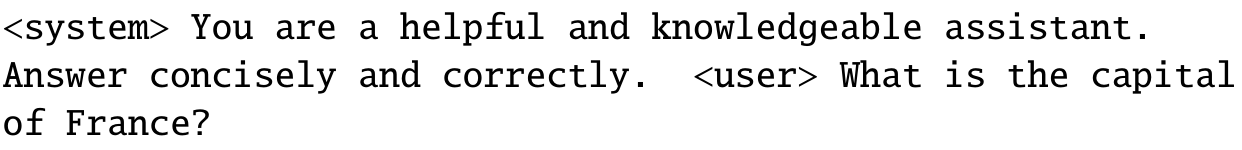
\includegraphics[width=0.7\textwidth]{bab2/exsystemprompt.png}
\caption[Contoh \textit{System Prompt}]{Contoh penggunaan \textit{System Prompt} dalam interaksi dengan model bahasa \parencite{jm3}}
\label{fig:system_prompt}
\end{figure}

\subsection{\textit{Chain-of-Thought}}
\textit{Chain-of-Thought} (CoT) \textit{prompting} merupakan teknik yang diperkenalkan oleh \textcite{weiChainofThoughtPromptingElicits2023} untuk meningkatkan kemampuan penalaran kompleks pada \textit{Large Language Models} (LLM). Metode ini mengarahkan model untuk menghasilkan serangkaian langkah penalaran perantara (\textit{intermediate reasoning steps}) sebelum menyajikan jawaban akhir, menyerupai proses kognitif manusia dalam memecahkan masalah yang rumit secara bertahap.

Dalam paradigma \textit{prompting} standar, model umumnya dilatih untuk memprediksi jawaban secara langsung dari masukan yang diberikan \parencite{weiChainofThoughtPromptingElicits2023}. Pendekatan tersebut sering kali menghasilkan kesalahan pada tugas-tugas yang memerlukan logika bertingkat, seperti soal cerita matematika atau penalaran simbolis. Sebaliknya, CoT memungkinkan model untuk menguraikan masalah menjadi komponen-komponen yang lebih kecil, sehingga mengurangi kemungkinan kesalahan logika pada hasil akhir. Perbedaan fundamental antara pendekatan standar dan CoT divisualisasikan pada Gambar \ref{fig:cot_comparison}.

\begin{figure}[H]
\centering
\includegraphics[width=0.6\textwidth]{bab2/cotcomparison.png}
\caption[Perbandingan \textit{standard prompting} dan \textit{chain-of-thought prompting}]{Perbandingan \textit{standard prompting} dan \textit{chain-of-thought prompting} dalam menyelesaikan soal cerita matematika \parencite{weiChainofThoughtPromptingElicits2023}}
\label{fig:cot_comparison}
\end{figure}

Penerapan CoT dapat dilakukan melalui dua strategi utama. Strategi pertama adalah \textit{Few-Shot CoT}, di mana \textit{prompt} diperkaya dengan sejumlah contoh demonstrasi (\textit{exemplars}) yang secara eksplisit menampilkan alur penalaran beserta jawabannya \parencite{weiChainofThoughtPromptingElicits2023}. Strategi kedua adalah \textit{Zero-Shot CoT} yang diusulkan oleh \textcite{kojimaLargeLanguageModels2023}. Pada strategi ini, kemampuan penalaran model diaktifkan hanya dengan menambahkan instruksi pemicu seperti "Mari berpikir langkah demi langkah" (\textit{"Let's think step by step"}) tanpa memerlukan contoh demonstrasi spesifik. Temuan ini mengindikasikan bahwa kapasitas penalaran merupakan kemampuan inheren yang dimiliki oleh LLM berskala besar, yang dapat dimunculkan melalui instruksi yang tepat.

\subsection{\textit{Reasoning and Acting}}
\textit{Reasoning and Acting} (ReAct) merupakan pola yang mengatur cara kerja \textit{Large Language Model} (LLM). Pola ini pertama kali diperkenalkan oleh \textcite{yaoReActSynergizingReasoning2023} sebagai sebuah teknik \textit{prompting} dalam \textit{prompt engineering}. ReAct memberikan \textit{prompt} yang mengarahkan LLM untuk menghasilkan jejak pemikiran sekaligus melaksanakan tindakan yang spesifik terhadap suatu tugas secara bersamaan. Melalui mekanisme tersebut, sistem mampu melakukan penalaran dinamis untuk menyusun, menjaga, dan menyesuaikan rencana tindakan, sekaligus berinteraksi dengan lingkungan eksternal, misalnya dengan melakukan pencarian tambahan melalui API atau basis data sebelum menggunakan hasilnya untuk mengambil keputusan yang lebih tepat. 

Dalam implementasinya, \textcite{yaoReActSynergizingReasoning2023} menggunakan \textit{prompt} untuk menginstruksikan LLM menghasilkan tindakan dalam skema atau struktur yang telah ditentukan, yang salah satunya dapat berupa pemanggilan (API). Dari struktur ini, lingkungan eksternal bertugas mengekstraksi pemanggilan API tersebut untuk dieksekusi pada kode alat yang sebenarnya. Gambar \ref{fig:react_illustration} memperlihatkan ilustrasi mekanisme ReAct dalam menjawab pertanyaan pada dataset HotpotQA dari \textcite{yangHotpotQADatasetDiverse2018}. Dalam ilustrasi tersebut, model berusaha mengidentifikasi perangkat lain yang dapat digunakan untuk mengontrol program menggunakan Apple Remote.

\begin{figure}[H]
\centering
\includegraphics[width=0.7\textwidth]{bab2/ilustrasireact.png}
\caption[Ilustrasi metode ReAct]{Ilustrasi metode ReAct dalam menyelesaikan tugas \parencite{yaoReActSynergizingReasoning2023}}
\label{fig:react_illustration}
\end{figure}

ReAct merupakan pengembangan dari teknik \textit{prompting} \textit{Chain-of-Thought} (CoT) dari \textcite{weiChainofThoughtPromptingElicits2023}, yang memungkinkan model menghasilkan jejak penalaran (\textit{reasoning traces}) untuk menjawab pertanyaan yang melibatkan aritmatika, penalaran berbasis logika, maupun \textit{commonsense reasoning}. Akan tetapi, CoT memiliki keterbatasan karena tidak dapat mengakses informasi eksternal atau memperbarui pengetahuannya, sehingga sering menimbulkan masalah seperti halusinasi fakta dan propagasi kesalahan. Pada penelitian \textcite{yaoReActSynergizingReasoning2023}, ReAct dan CoT dievaluasi pada dataset HotpotQA \parencite{yangHotpotQADatasetDiverse2018} untuk tugas tanya jawab dan FEVER \parencite{thorneFEVERLargescaleDataset2018} untuk verifikasi fakta, dengan menggunakan PaLM-540B sebagai model dasar. Hasil evaluasi menunjukkan bahwa ReAct secara umum memberikan kinerja lebih baik dibandingkan Act (yang hanya melibatkan tindakan) pada kedua tugas, dengan skor 27,4 pada HotpotQA dan 58,9 pada FEVER untuk ReAct, serta 25,7 dan 58,9 untuk Act. ReAct juga melampaui CoT pada FEVER dengan skor 60,9, meskipun masih tertinggal pada HotpotQA dengan skor 27,4 dibandingkan 33,4 untuk CoT.

Analisis lebih lanjut oleh \textcite{yaoReActSynergizingReasoning2023} menunjukkan bahwa CoT rentan terhadap halusinasi fakta, sementara ReAct memiliki keterbatasan fleksibilitas karena adanya struktur langkah yang kaku dalam merumuskan penalaran. Selain itu, ReAct sangat bergantung pada kualitas informasi yang diambil. Jika hasil pencarian tidak relevan, proses penalaran model dapat terganggu dan sulit untuk dipulihkan. Menariknya, ketika CoT dan ReAct dikombinasikan melalui mekanisme yang memungkinkan model beralih di antara keduanya, kinerjanya melampaui semua metode \textit{prompting} lain, dengan skor 35,1 pada HotpotQA dan 64,6 pada FEVER. Hasil ini memperlihatkan bahwa kekurangan ReAct dapat ditutupi oleh keunggulan CoT, sehingga kombinasi keduanya menghasilkan sistem yang lebih akurat.

\section{\textit{Object Detection}}
Deteksi objek adalah salah satu tugas fundamental dalam \textit{computer vision} yang bertujuan untuk mengidentifikasi keberadaan objek tertentu dalam citra digital dan menentukan lokasi tepatnya \parencite{raniObjectDetectionRecognition2022}. Berbeda dengan pengenalan gambar (\textit{image recognition}) atau klasifikasi citra yang hanya memberikan label kategori tunggal untuk keseluruhan gambar, deteksi objek memberikan informasi yang lebih granular berupa label kelas dan koordinat kotak pembatas untuk setiap instansi objek yang ditemukan. Perbedaan visual antara pengenalan gambar dan deteksi objek dapat dilihat pada Gambar \ref{fig:obj_vs_recog}.

\begin{figure}[H]
\centering
\includegraphics[width=0.4\textwidth]{bab2/Image-recognition-vs-object-detection.png}
\caption[Perbedaan Antara \textit{Image Recognition} dan \textit{Object Detection}]{Perbedaan Antara \textit{Image Recognition} dan \textit{Object Detection} \parencite{raniObjectDetectionRecognition2022}}
\label{fig:obj_vs_recog}
\end{figure}

Berdasarkan cakupan kategori objek yang dapat dikenali, sistem deteksi objek secara umum diklasifikasikan menjadi dua paradigma, yaitu \textit{closed-set object detection} (CSOD) dan \textit{open-vocabulary object detection} (OVD) \parencite{hosoyaOpenvocabularyVsClosedset2024}. CSOD merupakan pendekatan konvensional di mana model dilatih menggunakan dataset dengan daftar kategori yang telah ditentukan sebelumnya . Model jenis ini hanya mampu mendeteksi objek yang termasuk dalam kategori pelatihan tersebut dan akan memperlakukan objek lain sebagai latar belakang. Sebaliknya, OVD bertujuan untuk mengatasi keterbatasan ini dengan memanfaatkan kemampuan generalisasi dari model bahasa-visi. Pendekatan ini memungkinkan model untuk mendeteksi objek berdasarkan deskripsi teks bebas, termasuk kategori objek yang tidak pernah dilihat selama proses pelatihan. Perbedaan mekanisme antara kedua pendekatan ini diilustrasikan pada Gambar \ref{fig:closed_vs_open}.

\begin{figure}[H]
\centering
\includegraphics[width=\textwidth]{bab2/closedsetvsopenvocab.png}
\caption[Perbedaan \textit{closed-set} dan \textit{open-vocabulary object detection}]{Perbedaan \textit{closed-set} dan \textit{open-vocabulary object detection} \parencite{hosoyaOpenvocabularyVsClosedset2024}}
\label{fig:closed_vs_open}
\end{figure}

\subsection{\textit{You Only Look Once}}
\textit{You Only Look Once} (YOLO) merupakan algoritma deteksi objek yang pertama kali diperkenalkan oleh \textcite{redmonYouOnlyLook2016a} melalui pendekatan yang menyatukan proses prediksi lokasi objek dan klasifikasi dalam satu jaringan saraf tunggal. Dalam bidang \textit{computer vision}, deteksi objek merupakan tugas krusial yang bertujuan untuk mengidentifikasi jenis objek sekaligus menentukan posisinya dalam citra melalui koordinat \textit{bounding box}. Sebelum kemunculan YOLO, deteksi objek didominasi oleh pendekatan \textit{two-stage detector} seperti Faster R-CNN yang dikembangkan oleh \textcite{renFasterRCNNRealTime2017}. Visualisasi arsitektur dasar YOLO diilustrasikan pada Gambar \ref{fig:yolo_architecture}.

\begin{figure}[H]
\centering
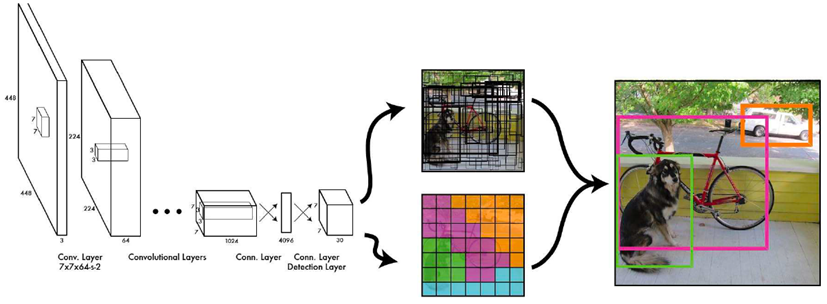
\includegraphics[width=0.8\textwidth]{bab2/arsitekturyolo.png}
\caption[Arsitektur YOLO]{Arsitektur YOLO \parencite{redmonYouOnlyLook2016a}}
\label{fig:yolo_architecture}
\end{figure}

Perbedaan utama antara kedua pendekatan tersebut terletak pada alur pemrosesannya. \textit{Two-stage detector} bekerja dengan menghasilkan sejumlah usulan wilayah (\textit{region proposals}) terlebih dahulu, baru kemudian melakukan klasifikasi pada setiap wilayah tersebut secara terpisah \Parencite{renFasterRCNNRealTime2017}. Meskipun akurat, proses ini memerlukan waktu komputasi yang besar sehingga sulit digunakan untuk aplikasi yang membutuhkan respons cepat. Sebaliknya, YOLO sebagai \textit{one-stage detector} memperlakukan deteksi objek sebagai masalah regresi tunggal, yang memetakan piksel gambar langsung ke koordinat \textit{bounding box} dan probabilitas kelas dalam satu kali jalan (\textit{one-pass}) \parencite{redmonYouOnlyLook2016a}. Karakteristik ini memungkinkan YOLO untuk bekerja secara \textit{real-time} dengan kecepatan yang jauh mengungguli pendahulunya.

Perkembangan arsitektur YOLO terus mengalami peningkatan signifikan sejak pertama kali dirilis. Setelah versi awal oleh \textcite{redmonYouOnlyLook2016a}, berbagai iterasi seperti YOLOv2 \parencite{redmonYOLO9000BetterFaster2016}, YOLOv3 \parencite{redmonYOLOv3IncrementalImprovement2018}, hingga YOLOv7 \parencite{wangYOLOv7TrainableBagofFreebies2023} membawa peningkatan pada akurasi dan kecepatan melalui teknik-teknik seperti \textit{anchor boxes}, \textit{feature pyramid networks}, dan optimalisasi \textit{backbone}. Saat ini, pengembangan YOLO dikelola secara luas oleh Ultralytics \parencite{jocherUltralyticsYOLO2023}, yang telah merilis versi populer seperti YOLOv8 dan YOLOv9 \parencite{wangYOLOv9LearningWhat2025}. Iterasi terbaru ini mengintegrasikan kemajuan terbaru dalam \textit{deep learning}, seperti penggunaan \textit{backbone} yang lebih efisien serta modul \textit{neck} yang mampu menangkap fitur pada berbagai skala dengan lebih baik.

Versi terbaru yang diperkenalkan oleh Ultralytics adalah YOLOv11, yang membawa sejumlah pembaruan arsitektur untuk meningkatkan efisiensi ekstraksi fitur dan performa deteksi \parencite{khanamYOLOv11OverviewKey2024}. Arsitektur YOLOv11 memperkenalkan blok C3k2 yang merupakan evolusi dari modul C2f, serta penggunaan \textit{Spatial Pyramid Pooling - Fast} (SPPF) yang dioptimalkan untuk mempercepat pemrosesan tanpa mengurangi kualitas representasi spasial. Selain itu, integrasi modul \textit{Cross-Stage Partial with Shared Attention} (C2PSA) pada bagian \textit{neck} memungkinkan model untuk lebih fokus pada fitur-fitur penting dalam citra, sehingga meningkatkan akurasi pada objek dengan skala yang bervariasi. Visualisasi arsitektur YOLOv11 secara mendetail dapat dilihat pada Gambar \ref{fig:yolov11_architecture}.

\begin{figure}[H]
\centering
\includegraphics[width=0.9\textwidth]{bab2/yolov11architecture.png}
\caption[Arsitektur YOLOv11]{Arsitektur YOLOv11 \parencite{sapkotaYOLOAdvancesIts2025}}
\label{fig:yolov11_architecture}
\end{figure}

Dari sisi performa, YOLOv11 menunjukkan peningkatan efisiensi komputasi yang signifikan dibandingkan dengan versi sebelumnya. Berdasarkan hasil pengujian pada dataset COCO, YOLOv11 mampu mencapai nilai \textit{mean Average Precision} (mAP) yang lebih tinggi dengan jumlah parameter yang lebih sedikit jika dibandingkan dengan YOLOv8 dan YOLOv10 \parencite{khanamYOLOv11OverviewKey2024}. Hal ini membuat YOLOv11 sangat kompetitif untuk aplikasi \textit{real-time} yang membutuhkan keseimbangan antara akurasi tinggi dan latensi rendah. Perbandingan performa YOLOv11 terhadap iterasi YOLO sebelumnya diilustrasikan pada Gambar \ref{fig:yolov11_benchmark}.

\begin{figure}[H]
\centering
\includegraphics[width=0.8\textwidth]{bab2/yolov11benchmark.png}
\caption[Perbandingan performa YOLOv11]{Perbandingan performa YOLOv11 terhadap model YOLO lainnya \parencite{khanamYOLOv11OverviewKey2024}}
\label{fig:yolov11_benchmark}
\end{figure}

Saat ini, Ultralytics memposisikan YOLO11 sebagai versi yang paling stabil dan efisien untuk berbagai skenario penggunaan \parencite{jocherUltralyticsYOLO2023}, meskipun versi YOLOv12 telah mulai diperkenalkan oleh \textcite{tianYOLOv12AttentionCentricRealTime2025}. Peningkatan arsitektur pada YOLO11 difokuskan pada pengoptimalan aliran informasi dalam jaringan guna mengurangi beban komputasi tanpa mengorbankan akurasi. Hal ini dapat dibuktikkan berdasarkan hasil evaluasi kinerja yang dilakukan oleh \textcite{sapkotaComprehensivePerformanceEvaluation2026} pada deteksi objek di lingkungan pertanian yang kompleks, YOLO11 menunjukkan konsistensi performa yang lebih baik dibandingkan dengan varian YOLOv8 hingga YOLOv12. Dalam pengujian tersebut, varian terkecil yakni YOLO11n (\textit{nano}) tercatat memiliki kecepatan pemrosesan paling tinggi dibandingkan model lainnya, yang menjadikannya sangat ideal untuk implementasi pada perangkat dengan keterbatasan sumber daya. Hasil perbandingan kinerja dari berbagai varian YOLO tersebut disajikan pada Tabel \ref{tab:yolo_benchmark}.

{
\setstretch{1.0}
\begin{longtblr}[
    caption = {Hasil \textit{benchmark} berbagai varian YOLO pada tugas deteksi objek di lingkungan pertanian oleh \textcite{sapkotaComprehensivePerformanceEvaluation2026}},
    entry = {Hasil \textit{benchmark} berbagai varian YOLO},
    label = {tab:yolo_benchmark},
]{
    width = \linewidth,
    colspec = {X[1.5,l] *{3}{X[1,c]}},
    hlines, vlines,
    rows = {m},
    rowsep = 4pt,
    row{1} = {font=\bfseries, halign=c, valign=m},
    rowhead = 1,
}
    Model & Pre (ms) & Inf (ms) & Post (ms) \\
    \SetCell[c=4]{l} \textit{YOLOv8} & & & \\
    YOLOv8n & 1.3 & 4.1 & 2.3 \\
    YOLOv8s & 1.3 & 6.4 & 2.3 \\
    YOLOv8m & 1.3 & 11.2 & 2.1 \\
    YOLOv8l & 1.2 & 18.7 & 2.2 \\
    YOLOv8x & 0.9 & 24.8 & 2.3 \\
    \SetCell[c=4]{l} \textit{YOLOv9} & & & \\
    YOLOv9-t & 1.3 & 14.1 & 2.2 \\
    YOLOv9-s & 1.3 & 11.5 & 2.2 \\
    YOLOv9-m & 1.3 & 14.0 & 2.1 \\
    YOLOv9-c & 1.3 & 17.0 & 2.0 \\
    YOLOv9-b & 1.2 & 17.2 & 2.0 \\
    YOLOv9-e & 1.1 & 33.5 & 1.9 \\
    \SetCell[c=4]{l} \textit{YOLOv10} & & & \\
    YOLOv10n & 1.4 & 5.5 & 1.6 \\
    YOLOv10s & 1.3 & 7.7 & 1.6 \\
    YOLOv10m & 1.3 & 13.0 & 1.6 \\
    YOLOv10b & 1.3 & 16.7 & 1.5 \\
    YOLOv10l & 1.4 & 19.6 & 1.5 \\
    YOLOv10x & 1.2 & 26.5 & 1.5 \\
    \SetCell[c=4]{l} \textit{YOLOv11} & & & \\
    YOLOv11n & \textbf{0.1} & \textbf{2.4} & 2.2 \\
    YOLOv11s & \textbf{0.1} & 5.0 & 2.5 \\
    YOLOv11m & \textbf{0.1} & 11.9 & 0.6 \\
    YOLOv11l & 0.2 & 14.6 & 1.2 \\
    YOLOv11x & \textbf{0.1} & 26.3 & 0.6 \\
    \SetCell[c=4]{l} \textit{YOLOv12} & & & \\
    YOLOv12n & 0.8 & 4.6 & 0.7 \\
    YOLOv12s & 3.8 & 9.6 & 1.0 \\
    YOLOv12m & 0.3 & 15.9 & \textbf{0.5} \\
    YOLOv12l & 0.6 & 19.2 & \textbf{0.5} \\
\end{longtblr}
}
%NOTE: Perlu tambahin studi literatur penggunaan model YOLO biasanya sebagai bagian pertama dari two-stage detector

\subsection{OWLv2}
OWLv2 (\textit{Open-Vocabulary World Object Detection}) merupakan model OVD yang dikembangkan oleh \textcite{mindererScalingOpenVocabularyObject2024} untuk mendeteksi dan mengklasifikasikan objek berdasarkan deskripsi teks bebas. Kemampuan ini memberikan fleksibilitas tinggi dalam mengenali objek baru tanpa memerlukan pelatihan ulang. Pengembangan model ini berakar pada penelitian sebelumnya oleh \textcite{mindererSimpleOpenVocabularyObject2022} yang memperkenalkan OWL-ViT (\textit{Vision Transformer for Open-World Localization}). OWL-ViT mengadaptasi arsitektur \textit{Vision Transformer} (ViT) standar dengan sedikit modifikasi untuk tugas deteksi objek dan dilatih menggunakan pasangan gambar serta teks dalam skala besar. Pendekatan ini bertujuan mentransfer kemampuan pengenalan visual-semantik dari model seperti CLIP ke dalam tugas lokalisasi objek, sehingga menjembatani kesenjangan antara klasifikasi gambar tingkat tinggi dan deteksi objek yang lebih rinci melalui pencocokan fitur dari \textit{image encoder} dengan \textit{text embedding} dari \textit{query} label.

\textcite{mindererScalingOpenVocabularyObject2024} kemudian mengembangkan OWLv2 dengan fokus utama pada skalabilitas data pelatihan. Tantangan utama dalam OVD adalah kelangkaan data anotasi kotak pembatas (\textit{bounding box}) yang terkurasi. Untuk mengatasi hal ini, OWLv2 menerapkan strategi pelatihan mandiri (\textit{self-training}) yang memanfaatkan detektor yang sudah ada untuk menghasilkan label semu (\textit{pseudo-labels}) pada dataset gambar-teks berskala web (WebLI) yang sangat besar. Dengan cara ini, model dapat belajar dari miliaran contoh data yang bising namun kaya informasi, yang secara signifikan meningkatkan kemampuan deteksi \textit{zero-shot}.

Secara arsitektur, \textcite{mindererScalingOpenVocabularyObject2024} mengoptimalkan desain OWL-ViT pada OWLv2 dengan meningkatkan efisiensi pada komponen \textit{detection head} dan strategi pelatihan. Model ini menggunakan \textit{image encoder} untuk mengekstraksi representasi visual dan \textit{text encoder} untuk memproses \textit{query} teks menjadi \textit{embedding}. Interaksi antara kedua representasi ini memungkinkan model untuk memprediksi lokasi objek dan probabilitas kelasnya berdasarkan kesesuaian semantik. Arsitektur umum dari pendekatan ini diilustrasikan pada Gambar \ref{fig:owlv2_architecture}.

\begin{figure}[H]
\centering
\includegraphics[width=\textwidth]{bab2/arsitekturowlv2.png}
\caption[Arsitektur OWLv2]{Arsitektur OWLv2 yang menggunakan \textit{image encoder} dan \textit{text encoder} untuk OVD \parencite{mindererScalingOpenVocabularyObject2024}}
\label{fig:owlv2_architecture}
\end{figure}

Keunggulan performa OWLv2 dibuktikan melalui evaluasi komprehensif oleh \textcite{wuEvaluatingPerformanceOpenVocabulary2026} yang membandingkan berbagai model OVD terkini. Hasil studi tersebut menunjukkan bahwa OWLv2 secara konsisten mengungguli model serupa, seperti OWL-ViT dan Grounding DINO dalam hal akurasi deteksi dan kemampuan generalisasi pada kategori objek yang belum pernah dilihat sebelumnya. \citeauthor{wuEvaluatingPerformanceOpenVocabulary2026} menyoroti bahwa strategi skala besar yang diterapkan pada OWLv2 memberikan keuntungan signifikan dalam menangani variasi visual dan kompleksitas deskripsi teks dibandingkan pendekatan lainnya.


\section{\textit{Retrieval-Augmented Generation}}
\textit{Retrieval-Augmented Generation} (RAG) didefinisikan oleh \textcite{huyenAIEngineeringBuilding2025} sebagai teknik yang meningkatkan kemampuan generasi model melalui pengambilan informasi relevan dari sumber memori eksternal, seperti basis data internal atau internet. Pola pengambilan lalu generasi ini pertama kali diperkenalkan oleh \textcite{chenReadingWikipediaAnswer2017} dalam sistem yang memanfaatkan halaman Wikipedia untuk menjawab pertanyaan domain terbuka. Istilah RAG kemudian dikukuhkan oleh \textcite{lewisRetrievalaugmentedGenerationKnowledgeintensive2020} sebagai solusi untuk tugas-tugas intensif pengetahuan (\textit{knowledge-intensive tasks}) di mana kapasitas model tidak mencukupi untuk menampung seluruh informasi. Melalui pendekatan ini, hanya informasi yang paling relevan yang diambil dan dimasukkan ke dalam model, yang terbukti mampu menghasilkan respons yang lebih detail serta mengurangi risiko halusinasi.

Secara arsitektural, sistem RAG mengintegrasikan tiga komponen utama, yaitu \textit{Retrieval}, \textit{Augmentation}, dan \textit{Generation} \parencite{singhAgenticRetrievalAugmentedGeneration2025}. Komponen \textit{Retrieval} bertugas melakukan \textit{query}, yakni permintaan pencarian informasi, pada sumber data eksternal, seperti basis pengetahuan, API, atau basis data vektor. Komponen ini sering memanfaatkan pencarian vektor padat dan model berbasis \textit{Transformer} untuk meningkatkan presisi pengambilan serta relevansi semantik. Selanjutnya, komponen \textit{Augmentation} memproses data yang diambil dengan mengekstraksi dan meringkas informasi yang paling relevan agar selaras dengan konteks \textit{query}. Terakhir, komponen \textit{Generation} menggabungkan informasi tersebut dengan pengetahuan pra-latih LLM untuk menghasilkan respons yang koheren dan sesuai konteks. Komponen-komponen utama dalam arsitektur RAG ini diilustrasikan pada Gambar \ref{fig:rag_components}.

\begin{figure}[H]
\centering
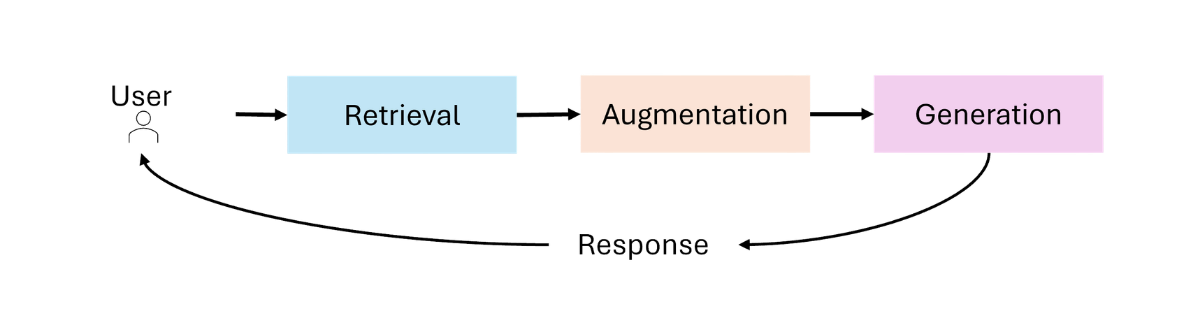
\includegraphics[width=0.8\textwidth]{bab2/rag_component.png}
\caption[Komponen inti arsitektur RAG]{Komponen inti arsitektur RAG \parencite{singhAgenticRetrievalAugmentedGeneration2025}}
\label{fig:rag_components}
\end{figure}

\textcite{huyenAIEngineeringBuilding2025} mengonseptualisasikan RAG sebagai mekanisme konstruksi konteks yang spesifik untuk setiap \textit{query}. Mekanisme ini membedakan RAG dari penggunaan konteks statis yang bersifat seragam. Walaupun jendela konteks model terus berkembang, RAG tetap relevan karena kemampuannya dalam menyeleksi informasi esensial secara efisien. Hal tersebut berdampak pada pengurangan biaya komputasi dan latensi dibandingkan dengan pemrosesan konteks yang sangat panjang secara keseluruhan.

\textcite{singhAgenticRetrievalAugmentedGeneration2025} dan \textcite{huyenAIEngineeringBuilding2025} mengemukakan bahwa paradigma pengembangan RAG dapat bervariasi bergantung pada kebutuhan spesifik aplikasi yang dibangun. Secara garis besar, \textcite{huyenAIEngineeringBuilding2025} mengklasifikasikan kerangka kerja RAG menjadi dua varian utama, yaitu \textit{Vanilla RAG} (atau \textit{Naive RAG}) dan \textit{Advanced RAG}. Karakteristik \textit{Vanilla RAG} menurut \textcite{singhAgenticRetrievalAugmentedGeneration2025} terletak pada kesederhanaan implementasinya yang sesuai untuk penanganan \textit{query} berbasis fakta dengan konteks yang tidak terlalu kompleks. Sebaliknya, \textit{Advanced RAG} mengintegrasikan teknik \textit{retrieval} yang lebih canggih untuk memenuhi kebutuhan aplikasi yang menuntut presisi tinggi serta pemahaman nuansa yang mendalam. Meskipun demikian, keterbatasan alur kerja statis pada kedua pendekatan tradisional tersebut mendorong munculnya paradigma baru, yakni \textit{Agentic RAG}. \textcite{singhAgenticRetrievalAugmentedGeneration2025} menjelaskan bahwa pendekatan ini mengintegrasikan agen otonom yang mampu melakukan pengambilan keputusan dinamis dan penalaran iteratif untuk mengatasi kendala pada paradigma sebelumnya. 

\subsection{\textit{Vanilla RAG}}

Sistem \textit{Vanilla RAG} terdiri dari tiga modul utama, yakni pipa ingesti (\textit{ingestion pipeline}), pipa pengambilan (\textit{retrieval pipeline}), dan pipa generasi (\textit{generation pipeline}). Modul ingesti berfungsi mengisi basis data vektor secara \textit{batch} atau \textit{streaming}, sementara modul pengambilan melakukan \textit{query} untuk mendapatkan entri relevan terhadap masukan pengguna. Modul generasi kemudian menggunakan data tersebut untuk memperkaya \textit{prompt} bagi LLM guna menghasilkan jawaban. Gambaran mengenai kerangka kerja \textit{Vanilla RAG} ini ditampilkan pada Gambar \ref{fig:naive_rag}.

\begin{figure}[H]
\centering
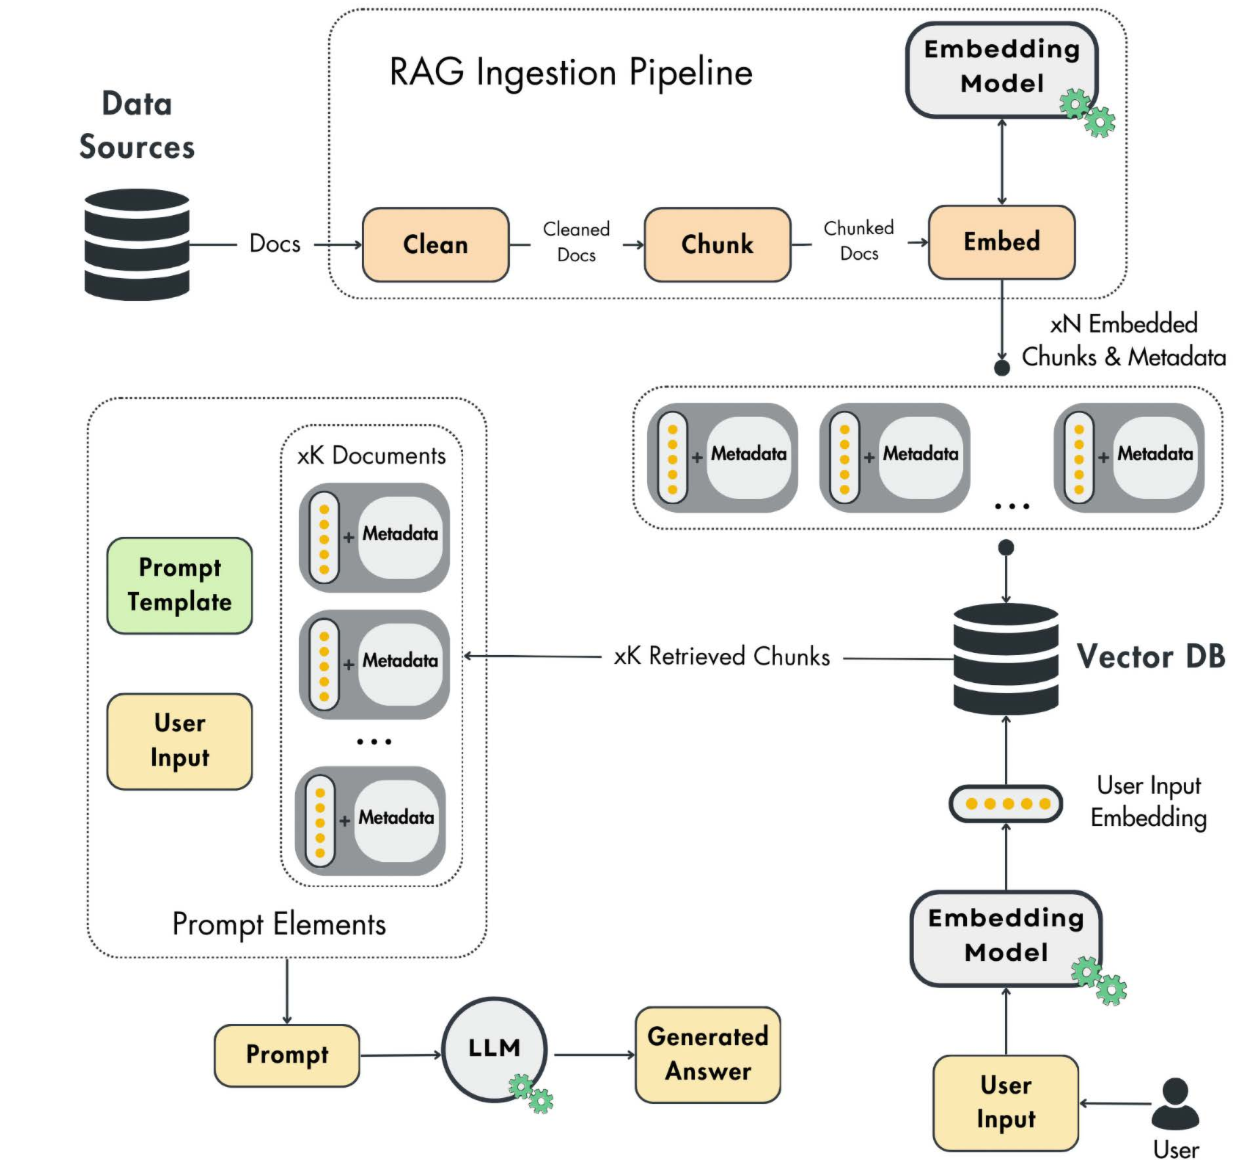
\includegraphics[width=0.7\textwidth]{bab2/naiverag.png}
\caption[Kerangka kerja \textit{Vanilla RAG}]{Kerangka kerja \textit{Vanilla RAG} yang terdiri dari pipa ingesti, pengambilan, dan generasi \parencite{iusztinLLMEngineersHandbook2024}}
\label{fig:naive_rag}
\end{figure}

\textcite{iusztinLLMEngineersHandbook2024} menjelaskan bahwa pipa ingesti bertugas mengekstraksi dokumen mentah dari berbagai sumber data, seperti \textit{data warehouse}, \textit{data lake}, atau halaman web. Data tersebut kemudian dibersihkan, dipecah menjadi bagian-bagian kecil (\textit{chunking}), dan diubah menjadi \textit{embedding} sebelum dimuat ke dalam basis data vektor. Tahapan pemrosesan data agar dapat ditemukan kembali dengan cepat ini oleh \textcite{huyenAIEngineeringBuilding2025} didefinisikan sebagai proses pengindeksan (\textit{indexing}). Lebih lanjut, \textcite{auffarthGenerativeAILangChain2025} menyatakan bahwa lapisan penyimpanan (\textit{storage layer}) yang menampung informasi eksternal setelah melalui proses pengindeksan ini dapat disebut sebagai basis pengetahuan (\textit{knowledge base}). Dalam konteks ini, \textcite{huyenAIEngineeringBuilding2025} juga mencatat bahwa istilah "dokumen" dan "\textit{chunk}" sering digunakan secara bergantian, karena secara teknis potongan dokumen juga merupakan sebuah dokumen tersendiri.

Pada tahap selanjutnya, komponen pengambilan memproses masukan pengguna, baik berupa teks, citra, maupun audio, dengan mengubahnya menjadi \textit{embedding} dan melakukan \textit{query} ke basis data vektor untuk mencari vektor yang serupa \parencite{iusztinLLMEngineersHandbook2024}. Fungsi utama dari langkah ini adalah memproyeksikan masukan pengguna ke dalam ruang vektor yang sama dengan indeks dokumen guna menemukan entri paling mirip (\textit{top-K}) sebagai konteks tambahan. Konteks yang diperoleh tersebut kemudian digabungkan dengan \textit{query} pengguna dalam sebuah \textit{template prompt} untuk diteruskan ke LLM pada tahap generasi. \textit{Prompt} akhir yang terbentuk merupakan hasil konstruksi dari \textit{template} sistem yang telah diisi dengan \textit{query} dan konteks relevan, di mana rekayasa \textit{prompt} (\textit{prompt engineering}) umumnya diterapkan pada level \textit{template} ini.

\subsection{\textit{Advanced RAG}}

\textcite{iusztinLLMEngineersHandbook2024} menyatakan bahwa kerangka kerja \textit{Vanilla RAG} masih memiliki keterbatasan dalam menangani aspek fundamental seperti relevansi dokumen, redundansi informasi, serta latensi sistem. Oleh sebab itu, kerangka kerja \textit{Advanced RAG} dikembangkan untuk mengoptimalkan proses tersebut melalui tiga tahapan utama, yaitu pra-pengambilan (\textit{pre-retrieval}), pengambilan (\textit{retrieval}), dan pasca-pengambilan (\textit{post-retrieval}). Tahap pra-pengambilan berfokus pada strukturisasi dan pemrosesan data guna memaksimalkan efisiensi pengindeksan serta \textit{query}. Tahap pengambilan bertujuan meningkatkan kualitas model \textit{embedding} dan strategi penyaringan metadata untuk memperbaiki hasil pencarian vektor. Sementara itu, tahap pasca-pengambilan menargetkan eliminasi gangguan (\textit{noise}) dari dokumen yang diambil serta kompresi \textit{prompt} sebelum diteruskan ke LLM. Sistem ini juga mensyaratkan adanya modul evaluasi yang kuat untuk mengukur kualitas data yang diambil dan jawaban yang dihasilkan secara kuantitatif. Gambaran mengenai kerangka kerja \textit{Advanced RAG} diperlihatkan pada Gambar \ref{fig:advanced_rag}.

\begin{figure}[H]
\centering
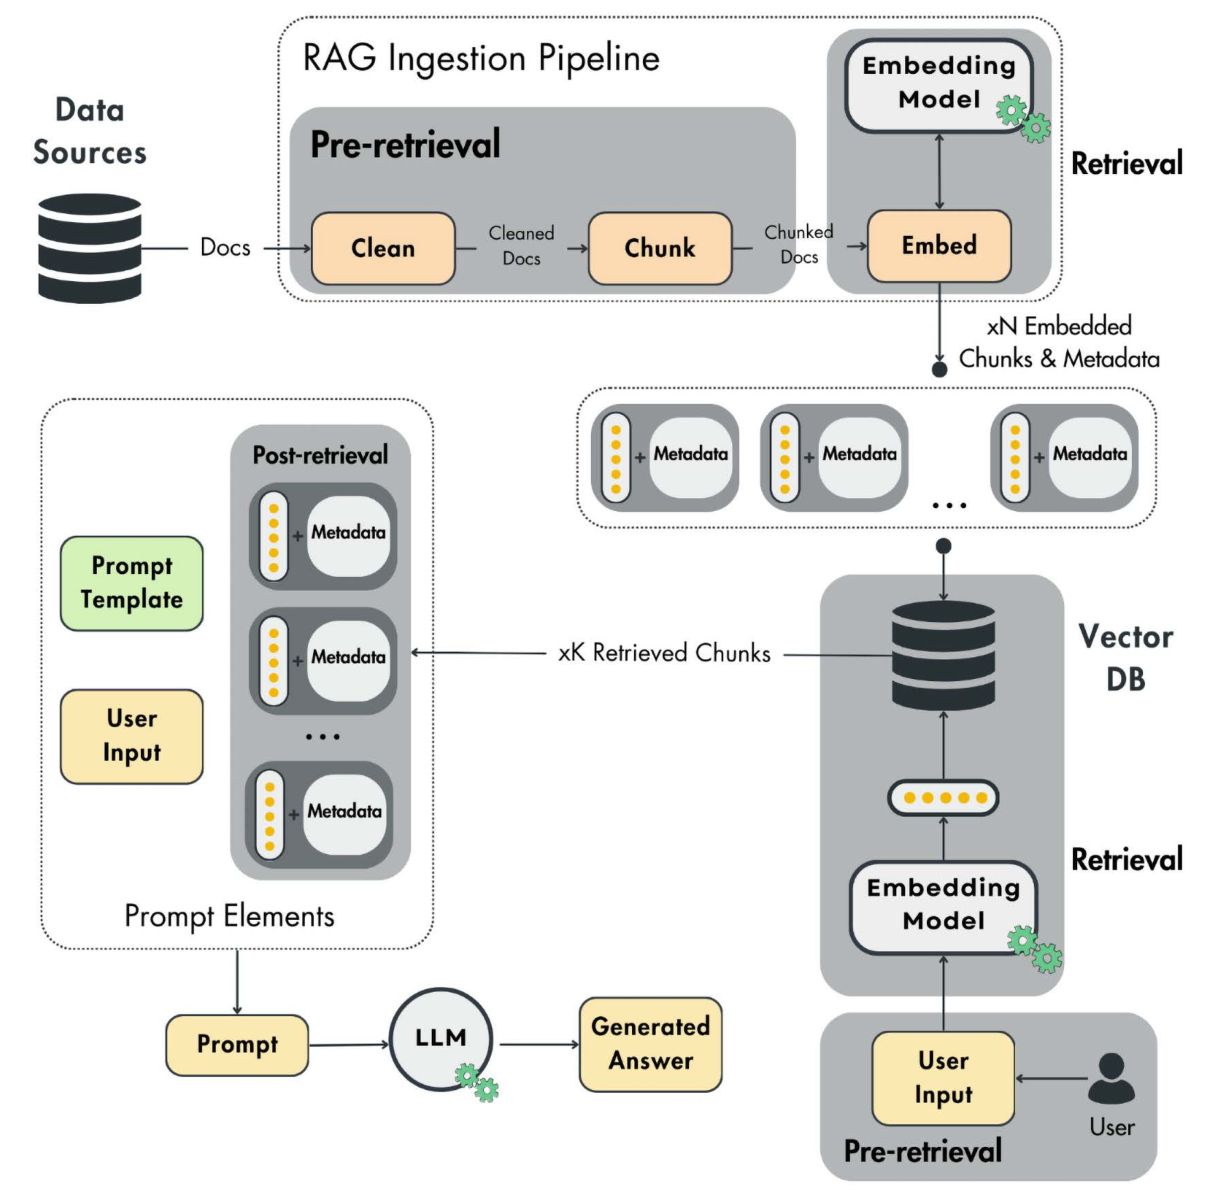
\includegraphics[width=\textwidth]{bab2/advancedrag.png}
\caption[Kerangka kerja \textit{Advanced RAG}]{Kerangka kerja \textit{Advanced RAG} yang terdiri dari tahapan pra-pengambilan, pengambilan, dan pasca-pengambilan \parencite{iusztinLLMEngineersHandbook2024}}
\label{fig:advanced_rag}
\end{figure}

Tahap pra-pengambilan dijalankan melalui dua pendekatan strategis, yakni pengindeksan data dan optimasi \textit{query} \parencite{iusztinLLMEngineersHandbook2024}. Pengindeksan data umumnya diimplementasikan pada modul pembersihan atau pemecahan data (\textit{chunking}) untuk memperbaiki struktur informasi, misalnya dengan menyematkan metadata berupa tanggal, URL, atau penanda bab. Metadata tersebut berperan krusial dalam memfasilitasi penyaringan data yang efisien saat proses pencarian berlangsung. Di sisi lain, optimasi \textit{query} berfokus pada penyempurnaan masukan pengguna agar lebih efektif saat diproses oleh sistem, salah satunya melalui teknik \textit{self-query}. Teknik ini memetakan \textit{query} tidak terstruktur menjadi bentuk terstruktur dengan bantuan LLM untuk mengidentifikasi entitas dan hubungan kunci sebagai parameter filter. Penggunaan parameter tersebut memungkinkan ruang pencarian vektor direduksi secara signifikan untuk meningkatkan relevansi hasil. \citeauthor{iusztinLLMEngineersHandbook2024} menekankan bahwa persiapan data dan \textit{query} yang matang ini merupakan fondasi bagi efisiensi tahapan selanjutnya.

Pada tahap pengambilan, optimasi dapat dicapai dengan meningkatkan kualitas model \textit{embedding} atau memanfaatkan fitur pencarian pada basis data \parencite{iusztinLLMEngineersHandbook2024}. Peningkatan model \textit{embedding} dilakukan untuk menangkap kemiripan semantik antara \textit{query} dan dokumen dengan lebih akurat pada saat inferensi. Pemanfaatan fitur basis data sering kali menjadi solusi yang lebih praktis, terutama melalui penerapan metode pencarian hibrida (\textit{hybrid search}). Metode ini menggabungkan pencarian berbasis kata kunci yang presisi dalam mencocokkan istilah spesifik dengan pencarian vektor yang unggul dalam menemukan kemiripan semantik. Selain itu, teknik pencarian vektor terfilter (\textit{filtered vector search}) juga dapat diterapkan dengan memanfaatkan indeks metadata untuk membatasi ruang pencarian sebelum atau sesudah pencarian vektor. Sinergi antara pencocokan kata kunci dan pemahaman semantik ini dinilai sangat efektif untuk tugas yang menuntut akurasi pengambilan informasi yang tinggi.

Tahap pasca-pengambilan difokuskan pada pemrosesan ulang data yang telah diambil untuk memastikan kinerja LLM tidak terganggu oleh konteks yang terlalu besar atau informasi yang tidak relevan \parencite{iusztinLLMEngineersHandbook2024}. Salah satu metode populer dalam tahap ini adalah \textit{reranking}, yang mengurutkan ulang dokumen menggunakan model \textit{machine learning} untuk memastikan hanya informasi yang paling relevan yang digunakan sebagai konteks akhir. Teknik-teknik optimasi ini merupakan contoh aspek yang dapat ditingkatkan dalam alur kerja RAG, namun penerapannya sangat bergantung pada jenis data yang dikelola. Teknik yang dirancang untuk teks mungkin tidak sepenuhnya dapat diterapkan pada data \textit{multimodal} seperti citra atau video yang memiliki karakteristik berbeda.

\subsection{\textit{Information Retrieval}}
Di balik layar, RAG menggunakan teknik \textit{Information Retrieval} (IR) untuk mengambil dokumen yang relevan guna menjawab pertanyaan \parencite{huyenAIEngineeringBuilding2025}. IR merupakan bidang yang mencakup pengambilan segala jenis media berdasarkan kebutuhan informasi pengguna \parencite{jm3}. Konsep ini merupakan gagasan yang telah berumur satu abad dan menjadi tulang punggung bagi mesin pencari, sistem rekomendasi, serta analitik \textit{log} \parencite{huyenAIEngineeringBuilding2025}. Banyak algoritma \textit{retrieval} yang dikembangkan untuk sistem pencarian tradisional tersebut juga dapat diterapkan dalam RAG. Sejarahnya dapat ditarik kembali hingga tahun 1920-an, saat Emanuel Goldberg mendeskripsikan "mesin statistik" dalam patennya untuk mencari dokumen yang tersimpan pada film \parencite{al-aminHistoryGenerativeArtificial2024}. 

Teknik IR yang umumnya digunakan dalam RAG adalah \textit{ad hoc retrieval}, di mana pengguna mengajukan \textit{query} kepada sistem pengambilan informasi dan sistem tersebut mengembalikan sekumpulan dokumen yang diurutkan berdasarkan relevansinya \parencite{jm3}. Dalam konteks ini, \textit{query} merepresentasikan kebutuhan informasi pengguna, dokumen merujuk pada satuan teks yang diindeks, dan koleksi merupakan kumpulan dokumen yang digunakan untuk memenuhi permintaan tersebut. Arsitektur umum sistem \textit{ad hoc retrieval} diilustrasikan pada Gambar \ref{fig:adhoc_ir}. Peringkat dokumen ditentukan dengan menghitung skor relevansi setiap dokumen kandidat terhadap \textit{query} yang diberikan, yang mengekspresikan seberapa relevan dokumen tersebut dalam memenuhi kebutuhan informasi pengguna. Secara umum, sistem IR ini terbagi menjadi dua kelas berdasarkan jenis vektor yang digunakan untuk merepresentasikan \textit{query} dan dokumen, yaitu \textit{sparse vector} dan \textit{dense vector}.

\begin{figure}[H]
\centering
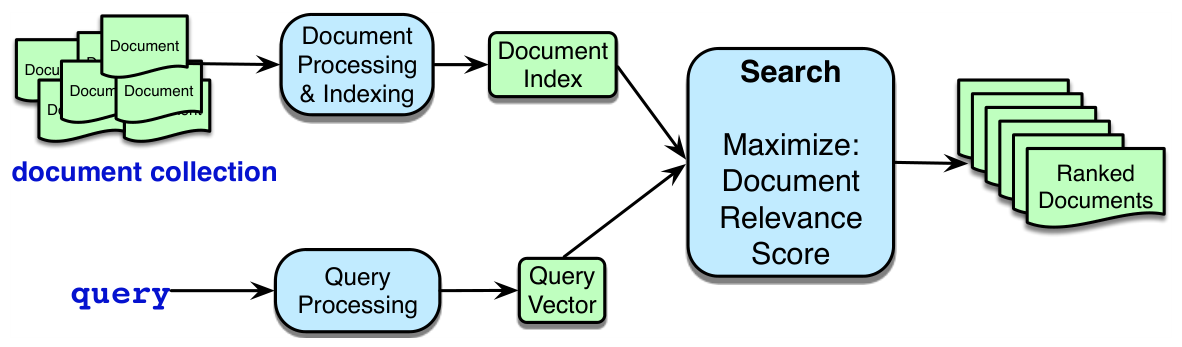
\includegraphics[width=0.9\textwidth]{bab2/adhoc-ir.png}
\caption[Arsitektur sistem \textit{ad hoc information retrieval}]{Arsitektur sistem \textit{ad hoc information retrieval} \parencite{jm3}}
\label{fig:adhoc_ir}
\end{figure}

\textit{Sparse retrieval}, yang juga disebut \textit{term-based retrieval} \parencite{huyenAIEngineeringBuilding2025} atau \textit{keyword-based retrieval} \parencite{auffarthGenerativeAILangChain2025}, bekerja pada level leksikal dengan mencocokkan istilah dalam \textit{query} secara langsung terhadap dokumen. Setiap kata dalam kosakata direpresentasikan sebagai \textit{one-hot vector} dengan ukuran sebesar panjang kosakata, sehingga representasi dokumen dan \textit{query} menjadi sangat jarang. Pendekatan ini mampu mencocokkan istilah-istilah spesifik secara tepat, namun cenderung gagal menangkap kesamaan semantik antara kata-kata yang bersinonim atau memiliki makna serupa.

\textit{Dense retrieval} di sisi lain mencocokkan dokumen berdasarkan kesamaan semantik antara \textit{query} dan dokumen, bukan sekadar tumpang tindih kata kunci \parencite{huyenAIEngineeringBuilding2025}. Pendekatan ini dikenal sebagai \textit{embedding-based retrieval}, karena representasi vektor padat dihasilkan oleh model \textit{embedding} yang menangkap makna semantik dari teks. Walaupun pembagian antara \textit{sparse} dan \textit{dense} tampak jelas, terdapat teknik yang berada di antara keduanya. Contohnya, \textcite{formalSPLADESparseLexical2021} memperkenalkan SPLADE (\textit{Sparse Lexical and Expansion}), algoritma pengambilan informasi yang menggunakan \textit{sparse embedding}. SPLADE memanfaatkan representasi dari model BERT dengan regularisasi untuk mendorong sebagian besar nilai \textit{embedding} menuju nol sehingga operasi menjadi lebih efisien, dan karena karakteristik \textit{sparse}-nya tersebut, SPLADE umumnya dikelompokkan bersama algoritma \textit{sparse retrieval}.

\subsubsection{\textit{Sparse Retrieval}}
\textit{Sparse retrieval} yang disebut juga \textit{lexical retrieval} merupakan pendekatan pencarian dokumen yang paling mendasar dengan memanfaatkan kata kunci dari \textit{query} \parencite{huyenAIEngineeringBuilding2025}. Metode ini bekerja dengan asumsi bahwa semakin sering suatu istilah muncul dalam sebuah dokumen, semakin relevan dokumen tersebut terhadap \textit{query} yang diberikan. Namun, ketergantungan semata pada frekuensi kemunculan kata (\textit{Term Frequency} atau TF) memiliki kelemahan signifikan, di mana kata-kata umum yang tidak informatif seperti kata penghubung dapat mendominasi skor relevansi. Untuk mengatasi hal ini, diperkenalkan konsep \textit{Inverse Document Frequency} (IDF) yang memberikan bobot lebih rendah pada kata yang muncul di banyak dokumen, sehingga sistem dapat memprioritaskan istilah yang lebih spesifik dan bermakna.

Algoritma TF-IDF menggabungkan kedua metrik tersebut untuk menghitung skor relevansi dokumen secara lebih akurat \parencite{huyenAIEngineeringBuilding2025}. Dalam mekanisme ini, nilai penting suatu kata berbanding terbalik dengan jumlah dokumen yang memuatnya. Secara matematis, skor total dokumen dihitung dengan menjumlahkan hasil perkalian antara IDF dan TF dari setiap kata yang terdapat dalam \textit{query}. Implementasi teknik ini umumnya memanfaatkan struktur data \textit{inverted index}, sebuah "kamus" yang memetakan istilah ke daftar dokumen yang memuatnya. Struktur ini memungkinkan pencarian teks yang sangat efisien sekaligus menyimpan metadata statistik yang diperlukan untuk perhitungan skor.

Salah satu varian TF-IDF yang paling banyak diadopsi dalam industri adalah Okapi BM25 yang pertama kali diperkenalkan oleh \textcite{harman1995trec3}. Algoritma ini menyempurnakan pendekatan TF-IDF standar dengan menambahkan normalisasi terhadap panjang dokumen dan saturasi frekuensi istilah \parencite{huyenAIEngineeringBuilding2025}. Normalisasi ini penting karena dokumen yang lebih panjang secara alami cenderung memuat lebih banyak kata kunci tanpa tentu lebih relevan. Meskipun metode \textit{retrieval} modern berbasis vektor semakin populer, BM25 dan variannya tetap menjadi standar industri yang kuat dan sering digunakan sebagai \textit{baseline} yang tangguh untuk membandingkan kinerja model pencarian yang lebih canggih.

\subsubsection{\textit{Dense Retrieval}}
Berbeda dengan \textit{sparse retrieval} yang bekerja pada level leksikal, \textit{dense retrieval} mencocokkan dokumen berdasarkan kesamaan semantik antara \textit{query} dan dokumen \parencite{huyenAIEngineeringBuilding2025}. Pendekatan ini, yang juga dikenal sebagai \textit{semantic retrieval} atau \textit{embedding-based retrieval}, menggunakan model \textit{embedding} untuk mengubah teks menjadi vektor padat yang merepresentasikan maknanya. Ketika suatu \textit{query} diajukan, \textit{query} tersebut diubah menjadi \textit{embedding} menggunakan model yang sama dengan yang dipakai saat pengindeksan, kemudian sistem mengambil $k$ potongan data yang vektornya paling dekat dengan vektor \textit{query}. Dengan demikian, \textit{dense retrieval} dapat menangani kasus di mana kata kunci dalam \textit{query} tidak muncul secara harfiah dalam dokumen yang relevan.

Pembentukan representasi vektor padat umumnya dilakukan menggunakan arsitektur \textit{Bi-Encoder} \parencite{jm3}. \textcite{reimersSentenceBERTSentenceEmbeddings2019} memperkenalkan Sentence-BERT (SBERT), sebuah modifikasi dari model BERT yang menggunakan jaringan siam (\textit{siamese network}) untuk menghasilkan \textit{embedding} kalimat yang bermakna secara semantik. Dalam arsitektur ini, dua input diproses secara paralel oleh model transformer dengan bobot yang sama (\textit{shared weights}), kemudian representasi keduanya dibandingkan menggunakan ukuran kesamaan seperti \textit{cosine similarity}, sebagaimana diilustrasikan pada Gambar \ref{fig:sentence_transformer}. Pendekatan ini memungkinkan komputasi kesamaan antar dokumen dalam skala besar secara efisien, berbeda dengan arsitektur \textit{Cross-Encoder} yang harus memproses pasangan teks secara bersamaan dan tidak praktis untuk pengindeksan skala besar.

\begin{figure}[H]
\centering
\includegraphics[width=0.6\textwidth]{bab2/sentencetransformer.png}
\caption[Arsitektur Sentence-BERT]{Arsitektur Sentence-BERT untuk menghasilkan \textit{embedding} kalimat \parencite{reimersSentenceBERTSentenceEmbeddings2019}}
\label{fig:sentence_transformer}
\end{figure}

Komponen krusial lain dalam \textit{dense retrieval} adalah basis data vektor (\textit{vector database}), yaitu basis data khusus yang dirancang untuk menyimpan dan mencari vektor \parencite{huyenAIEngineeringBuilding2025}. Pencarian vektor umumnya dirumuskan sebagai masalah \textit{nearest-neighbor search}: diberikan sebuah vektor \textit{query}, temukan $k$ vektor dalam basis data yang paling mirip berdasarkan metrik seperti \textit{cosine similarity}. Pendekatan naif $k$-NN yang menghitung kemiripan terhadap seluruh vektor dalam basis data memberikan hasil yang presisi, namun tidak efisien secara komputasi untuk dataset besar. Karena itu, pencarian vektor pada skala besar umumnya dilakukan menggunakan algoritma \textit{approximate nearest neighbor} yang menukar sedikit presisi dengan peningkatan kecepatan yang signifikan. Salah satu implementasi basis data vektor yang mendukung pencarian \textit{approximate nearest neighbor} adalah Qdrant \parencite{qdrantQdrant2025}.

Secara umum, basis data vektor mengorganisasi vektor ke dalam struktur seperti \textit{bucket}, pohon, atau graf untuk meningkatkan efisiensi pencarian \parencite{huyenAIEngineeringBuilding2025}. Salah satu algoritma \textit{approximate nearest neighbor} yang banyak digunakan adalah \textit{Hierarchical Navigable Small World} (HNSW), yang diperkenalkan oleh \textcite{malkovEfficientRobustApproximate2020}. HNSW membangun graf berlapis di mana setiap simpul merepresentasikan sebuah vektor, dan tepi-tepinya menghubungkan vektor-vektor yang berdekatan, sehingga pencarian \textit{nearest-neighbor} dilakukan dengan menelusuri tepi-tepi graf tersebut.

Walaupun basis data vektor muncul sebagai kategori tersendiri seiring berkembangnya RAG, pada dasarnya setiap basis data yang mampu menyimpan vektor dapat berfungsi sebagai basis data vektor \parencite{huyenAIEngineeringBuilding2025}. Saat ini, banyak basis data tradisional yang telah memperluas kapabilitasnya untuk mendukung penyimpanan dan pencarian vektor sebagai fitur tambahan. Fenomena ini menyebabkan batas klasifikasi antara basis data konvensional dan basis data vektor murni menjadi semakin kabur.

\subsection{\textit{Hybrid Search}}
\textit{Hybrid search} merupakan pendekatan yang menggabungkan beberapa metode \textit{retrieval} untuk memanfaatkan kelebihan masing-masing algoritma \parencite{huyenAIEngineeringBuilding2025}. Penggabungan ini dapat dilakukan secara berurutan maupun secara paralel sebagai \textit{ensemble}. Pada pendekatan berurutan, \textit{retriever} yang lebih ringan secara komputasi, seperti BM25, terlebih dahulu mengambil kandidat dokumen, kemudian hasil tersebut disaring lebih lanjut melalui tahap \textit{reranking} menggunakan pencarian vektor yang lebih presisi. Pada pendekatan paralel, beberapa \textit{retriever} dijalankan bersamaan, dan hasil peringkat dari masing-masing \textit{retriever} digabungkan menjadi peringkat akhir. Algoritma yang umum digunakan untuk menggabungkan peringkat dari beberapa \textit{retriever} adalah \textit{Reciprocal Rank Fusion} (RRF) dari \textcite{cormackReciprocalRankFusion2009}, di mana setiap dokumen mendapat skor berdasarkan posisi peringkatnya pada tiap \textit{retriever}, dan skor-skor tersebut dijumlahkan untuk menghasilkan peringkat akhir.

\subsection{\textit{Reranking}}
Peringkat dokumen awal yang dihasilkan oleh \textit{retriever} dapat disempurnakan lebih lanjut melalui proses \textit{reranking} \parencite{huyenAIEngineeringBuilding2025}. \textit{Reranking} bertujuan menghasilkan urutan dokumen yang lebih presisi sekaligus memungkinkan pengurangan jumlah dokumen yang diteruskan ke model, baik untuk menyesuaikan batas konteks model maupun mengurangi jumlah token masukan.Pada sistem \textit{dense retrieval}, \textit{retriever} umumnya menggunakan arsitektur \textit{bi-encoder} \parencite{jm3}. Pada arsitektur ini, dokumen di-\textit{encode} terlebih dahulu dan disimpan sebagai vektor, sehingga ketika \textit{query} masuk, hanya \textit{query} yang perlu di-\textit{encode} dan relevansinya dihitung menggunakan \textit{dot product} terhadap vektor dokumen yang telah tersimpan. Pendekatan ini efisien secara komputasi, namun kurang presisi karena tidak dapat menangkap sepenuhnya interaksi makna antar token antara \textit{query} dan dokumen akibat keduanya diproses secara independen.

Alternatif dari \textit{bi-encoder} adalah \textit{cross-encoder}, di mana \textit{query} dan dokumen dimasukkan sekaligus ke dalam \textit{Transformer} untuk menghasilkan skor relevansi \parencite{reimersSentenceBERTSentenceEmbeddings2019}. Karena kedua teks diproses bersamaan, \textit{cross-encoder} dapat memodelkan hubungan antar token secara langsung sehingga presisinya lebih tinggi. Akan tetapi, \textit{cross-encoder} tidak menghasilkan \textit{embedding} tersendiri dan setiap pasangan \textit{query}-dokumen harus diproses bersama, sehingga tidak praktis untuk digunakan langsung pada korpus besar. Perbandingan arsitektur keduanya diilustrasikan pada Gambar \ref{fig:biencoder_vs_crossencoder}.

\begin{figure}[H]
\centering
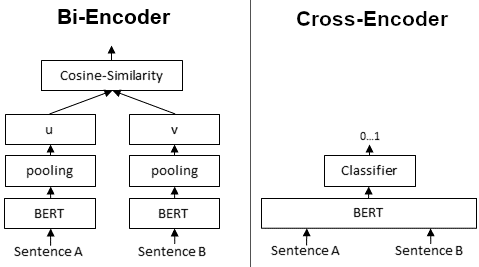
\includegraphics[width=0.7\textwidth]{bab2/biencoder_vs_crossencoder.png}
\caption[Perbandingan arsitektur \textit{bi-encoder} dan \textit{cross-encoder}]{Perbandingan arsitektur \textit{bi-encoder} dan \textit{cross-encoder} \parencite{reimersSentenceBERTSentenceEmbeddings2019}}
\label{fig:biencoder_vs_crossencoder}
\end{figure}

Dari karakteristik masing-masing arsitektur tersebut, pola umum dalam sistem \textit{reranking} adalah menggunakan \textit{bi-encoder} yang murah, namun kurang presisi untuk mengambil banyak kandidat dokumen pada tahap pertama guna memastikan \textit{recall}, kemudian mengurutkan ulang kandidat tersebut menggunakan \textit{cross-encoder} yang lebih mahal, namun lebih presisi untuk menghasilkan peringkat akhir \parencite{huyenAIEngineeringBuilding2025}. Sebagai alternatif \textit{cross-encoder}, ColBERT \parencite{khattabColBERTEfficientEffective2020} menawarkan pendekatan \textit{late interaction} yang berupaya menyeimbangkan biaya komputasi dan presisi. ColBERT mengenkode \textit{query} dan dokumen secara terpisah hingga representasi per token, menghasilkan sekumpulan vektor untuk setiap token yang dikenal sebagai \textit{multivectors}. Relevansi kemudian dihitung menggunakan operator \textit{MaxSim}, yaitu setiap token \textit{query} dicocokkan dengan token dokumen yang paling mirip, kemudian seluruh skor tersebut dijumlahkan. Karena \textit{multivectors} dokumen dapat disimpan sebelumnya, ColBERT dapat lebih efisien dari \textit{cross-encoder}. Cara kerja ColBERT diilustrasikan pada Gambar \ref{fig:colbert}.

\begin{figure}[H]
\centering
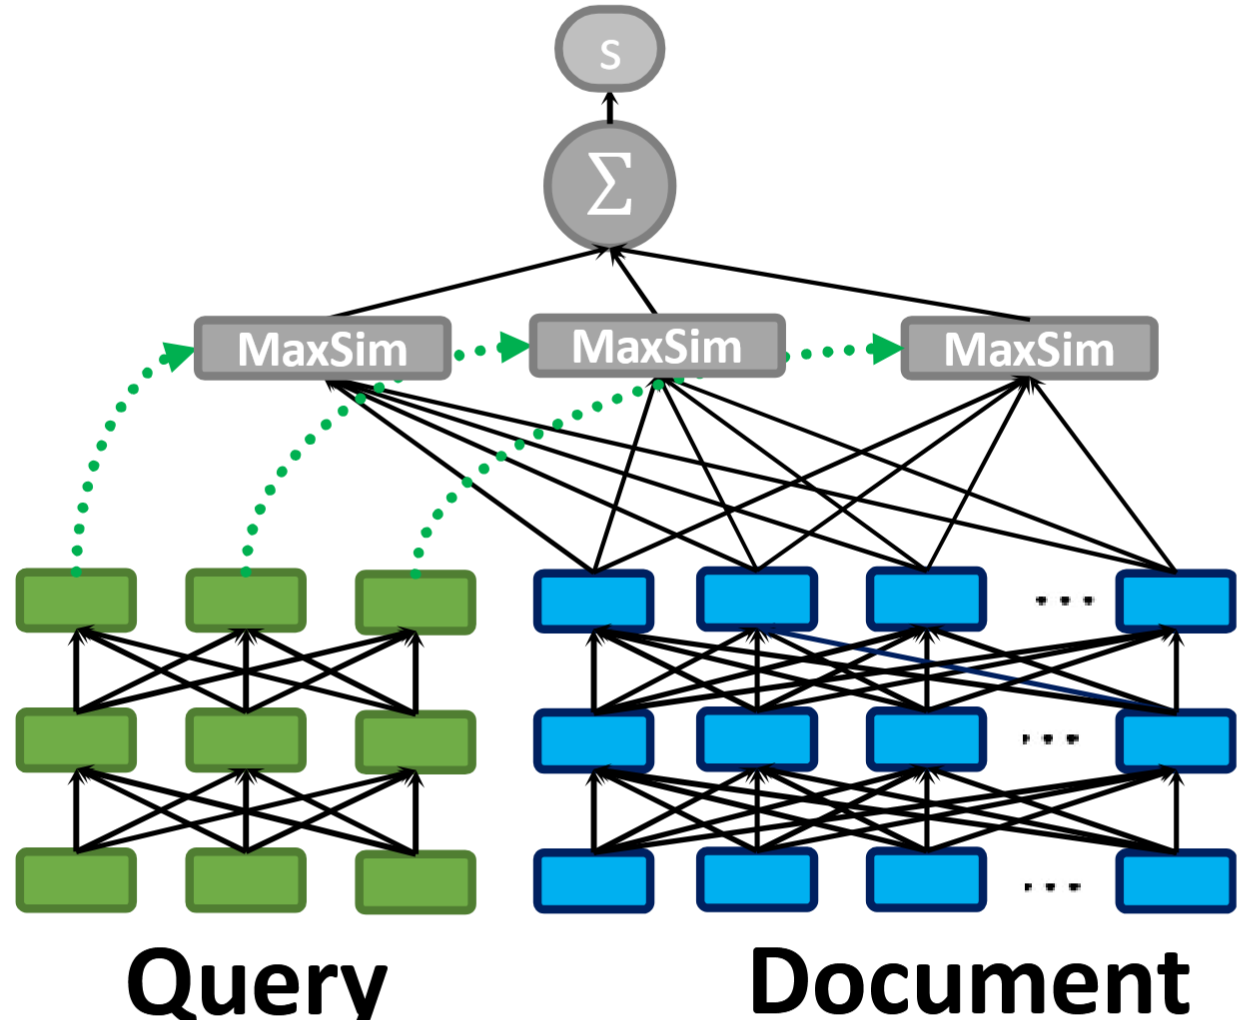
\includegraphics[width=0.4\textwidth]{bab2/colbert.png}
\caption[Ilustrasi mekanisme \textit{late interaction} pada ColBERT]{Ilustrasi mekanisme \textit{late interaction} pada ColBERT menggunakan operator \textit{MaxSim} \parencite{khattabColBERTEfficientEffective2020}}
\label{fig:colbert}
\end{figure}

\textcite{huyenAIEngineeringBuilding2025} juga menekankan bahwa \textit{reranking} dalam konteks RAG sedikit berbeda dari \textit{reranking} pada sistem pencarian konvensional. Pada sistem pencarian, posisi peringkat sangat menentukan karena pengguna cenderung memperhatikan hasil teratas. Dalam RAG, urutan dokumen dalam konteks tetap berpengaruh karena model cenderung lebih baik memproses informasi yang terletak di awal dan akhir konteks, sehingga penempatan dokumen yang paling relevan pada posisi tersebut dapat meningkatkan kualitas respons yang dihasilkan.

\subsection{Qdrant}
\textcite{qdrantQdrant2025} adalah \textit{library} (pustaka) \textit{open-source} (sumber terbuka) yang menyediakan mesin pencari vektor (\textit{vector search engine}) dan basis data vektor yang dirancang untuk menyimpan, mengelola, dan mencari vektor \textit{embedding} dalam skala besar dengan efisien. Qdrant menyediakan mekanisme pencarian kesamaan (\textit{similarity search}) melalui berbagai teknik IR dan algoritma pengambilan yang ada di industri.

Entitas utama yang menjadi unit penyimpanan dasar dalam \textcite{qdrantQdrant2025} dikenal sebagai \textit{Point}. Setiap \textit{Point} merepresentasikan catatan data tunggal yang terdiri dari tiga komponen utama, yaitu pengenal unik (ID), representasi vektor, dan \textit{payload} opsional. Struktur dari sebuah \textit{Point} dalam Qdrant diilustrasikan pada Gambar \ref{fig:qdrant_points}.

\begin{figure}[H]
\centering
\includegraphics[width=0.8\textwidth]{bab2/qdrantpoints.png}
\caption[Struktur Data \textit{Point} pada Qdrant]{Struktur Data \textit{Point} pada Qdrant yang Terdiri dari ID, Vektor, dan \textit{Payload} \parencite{qdrantQdrant2025}}
\label{fig:qdrant_points}
\end{figure}

Komponen ID pada struktur data \textcite{qdrantQdrant2025} berfungsi sebagai identitas unik untuk setiap \textit{Point}, yang dapat berupa bilangan bulat 64-bit (\textit{unsigned integer}) atau UUID. Jika pengguna tidak menyediakan ID saat pembuatan \textit{Point}, klien Qdrant secara otomatis akan menghasilkan UUID acak. Komponen kedua adalah vektor, yang merupakan representasi numerik dari data. Qdrant memiliki fleksibilitas tinggi dalam penyimpanan vektor, dengan dukungan terhadap berbagai jenis vektor seperti vektor padat (\textit{dense vector}), vektor jarang (\textit{sparse vector}), maupun \textit{multivector}. Lebih lanjut, Qdrant memungkinkan penyimpanan beberapa jenis vektor sekaligus dalam satu \textit{Point} melalui fitur \textit{named vectors}. Fitur ini berguna dalam skenario yang kompleks, seperti pada model \textit{multimodal} di mana satu entitas data mungkin memiliki representasi vektor untuk teks dan citra secara bersamaan.

Komponen terakhir pada struktur data \textcite{qdrantQdrant2025} adalah \textit{payload}, yang merupakan metadata tambahan dalam format JSON yang terkait dengan vektor tersebut. \textit{Payload} memungkinkan penyimpanan informasi non-vektor seperti atribut deskriptif, kategori, atau label waktu. Fungsi utama dari \textit{payload} adalah untuk memfasilitasi mekanisme penyaringan (\textit{filtering}) selama proses pencarian. Dengan fitur ini, Qdrant dapat melakukan pencarian hibrida yang menggabungkan pencarian semantik berbasis vektor dengan penyaringan berbasis aturan pada metadata, sehingga hasil yang diperoleh menjadi lebih spesifik dan relevan sesuai dengan kriteria yang diinginkan.

\subsection{Evaluasi Sistem \textit{Information Retrieval}}

Kualitas sebuah \textit{retriever} dapat dievaluasi berdasarkan kualitas data yang berhasil diambilnya \parencite{huyenAIEngineeringBuilding2025}. Dua metrik yang paling umum digunakan dalam evaluasi sistem IR adalah \textit{precision} dan \textit{recall} \parencite{jm3}. \textit{Precision} mengukur proporsi dokumen yang dikembalikan sistem yang benar-benar relevan, sedangkan \textit{recall} mengukur proporsi dokumen relevan yang berhasil ditemukan dari keseluruhan dokumen relevan yang tersedia. Untuk menghitung kedua metrik ini, dibutuhkan sebuah \textit{evaluation set} yang terdiri dari sekumpulan \textit{query} pengujian beserta dokumen yang telah dianotasi relevansinya, baik oleh manusia maupun \textit{AI judge} \parencite{huyenAIEngineeringBuilding2025}. Nilai \textit{precision} dan \textit{recall} kemudian dihitung berdasarkan hasil pengambilan \textit{retriever} pada \textit{evaluation set} tersebut.

Kedua metrik di atas tidak secara memadai mengukur kinerja sistem yang mengembalikan dokumen dalam urutan peringkat tertentu \parencite{jm3}. Penilaian berbasis \textit{precision} dan \textit{recall} tidak memperhitungkan posisi dokumen relevan dalam daftar hasil, padahal dokumen yang lebih relevan idealnya berada di posisi lebih atas. Untuk kasus seperti ini, metrik seperti NDCG (\textit{normalized discounted cumulative gain}) dan MRR (\textit{Mean Reciprocal Rank}) lebih tepat digunakan karena keduanya memperhitungkan urutan peringkat dalam penilaian kualitas pengambilan \parencite{huyenAIEngineeringBuilding2025}.

Seluruh metrik evaluasi IR tersebut dapat dihitung menggunakan ranx \parencite{bassaniRanxBlazingFastPython2022}, sebuah \textit{library} Python yang menyediakan berbagai metrik evaluasi peringkat secara cepat. ranx mendukung evaluasi \textit{offline} yang memanfaatkan \textit{ground truth} berupa pasangan \textit{query} dan dokumen relevan yang lazim disebut \textit{qrels} dalam IR. \textit{Library} ini mendukung seluruh metrik umum yang telah disebutkan, serta memungkinkan evaluasi beberapa \textit{run} dan metrik sekaligus dengan memparalelkan komputasi, sehingga cocok untuk evaluasi berskala besar.

\section{Sistem Agentik}
Menurut \textcite{anthropicBuildingEffectiveAgents2024}, sistem agentik (\textit{agentic system}) adalah pendekatan untuk memperluas kemampuan LLM dengan memberi akses pada alat, memori, atau sumber informasi eksternal sehingga model dapat bertindak lebih dari sekadar menghasilkan teks. Kemampuan \textit{foundation model} yang terus berkembang telah membuka kemungkinan bagi aplikasi-aplikasi agentik yang sebelumnya sulit diwujudkan \parencite{huyenAIEngineeringBuilding2025}. Paradigma ini umumnya dikenal dengan sebutan \textit{AI agent}, walaupun \textcite{anthropicBuildingEffectiveAgents2024} lebih memilih istilah sistem agentik untuk menekankan sifat sistemiknya. Konsep agen otonom sendiri bukan gagasan baru, di mana \textcite{russell2020artificial} secara eksplisit mendefinisikan kecerdasan buatan sebagai studi dan perancangan agen rasional, menjadikan agen cerdas yang otonom sebagai tujuan akhir dari bidang ini. Walaupun potensinya besar, \textcite{huyenAIEngineeringBuilding2025} mencatat bahwa sistem agentik berbasis AI masih merupakan bidang yang berkembang, dengan belum adanya kerangka teoretis yang mapan untuk mendefinisikan, mengembangkan, dan mengevaluasinya.

Secara struktural, sistem agentik terdiri dari empat komponen utama yang bekerja secara terintegrasi, sebagaimana diilustrasikan pada Gambar \ref{fig:komponen_sistem_agentik} \parencite{singhAgenticRetrievalAugmentedGeneration2025}. LLM dengan peran (\textit{role}) dan tugas (\textit{task}) yang terdefinisi berfungsi sebagai mesin penalaran utama yang menginterpretasikan \textit{query} pengguna dan menghasilkan respons. Memori dibagi menjadi memori jangka pendek (\textit{short-term memory}) untuk melacak konteks percakapan terkini, dan memori jangka panjang (\textit{long-term memory}) untuk menyimpan pengetahuan atau pengalaman yang terakumulasi. Komponen perencanaan (\textit{planning}) memandu proses penalaran sistem melalui mekanisme refleksi dan evaluasi mandiri (\textit{self-critique}) agar tugas-tugas kompleks dapat dipecah secara sistematis. Terakhir, alat-alat (\textit{tools}) seperti \textit{vector search}, \textit{web search}, dan API memperluas kemampuan sistem melampaui pembangkitan teks biasa, memungkinkan akses ke sumber data eksternal dan komputasi khusus.

\begin{figure}[H]
    \centering
    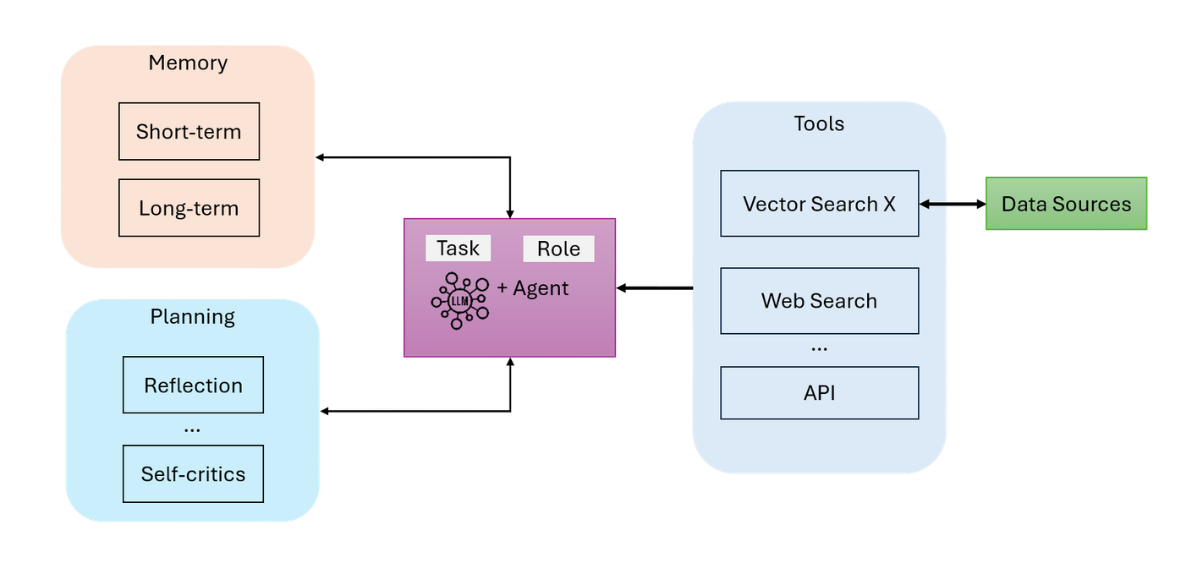
\includegraphics[width=0.85\textwidth]{bab2/arsitektur_sistem_agentik.png}
    \caption[Komponen-komponen sistem agentik]{Komponen-komponen sistem agentik yang terdiri dari LLM, memori, perencanaan, dan alat \parencite{singhAgenticRetrievalAugmentedGeneration2025}}
    \label{fig:komponen_sistem_agentik}
\end{figure}


\textcite{anthropicBuildingEffectiveAgents2024} membuat pembedaan arsitektur yang penting dalam sistem agentik antara \textit{workflow} dan \textit{agent}. \textit{Workflow} adalah sistem di mana LLM dan alat diatur melalui jalur kode yang telah ditentukan sebelumnya, sedangkan \textit{agent} adalah sistem di mana LLM secara dinamis mengarahkan proses dan penggunaan alatnya sendiri untuk menyelesaikan tugas. Pembedaan ini bukan bersifat preskriptif, melainkan merupakan pola-pola umum yang dapat dikombinasikan dan disesuaikan dengan kebutuhan kasus penggunaan yang berbeda \parencite{anthropicBuildingEffectiveAgents2024}.

\textcite{anthropicBuildingEffectiveAgents2024} mengenalkan beberapa pola \textit{workflow} yang umum dalam pengembangan sistem agentik. Pola \textit{prompt chaining} menyusun pemanggilan LLM secara berurutan, di mana \textit{output} satu tahap menjadi \textit{input} tahap berikutnya, seperti yang diterapkan \textcite{trautmannLargeLanguageModel2023} untuk memproses dokumen hukum melalui tahap peringkasan, pencarian semantik, hingga klasifikasi berbasis LLM. Pola \textit{routing} mengklasifikasikan \textit{input} lalu mengarahkannya ke alat atau proses yang sesuai, seperti yang digunakan \textcite{xuMultimodalAgriculturalAgent2025} dengan model klasifikasi sebagai \textit{router} untuk menentukan alat yang relevan berdasarkan gambar dan pertanyaan yang diterima. Pola \textit{parallelization} memungkinkan beberapa LLM memproses \textit{subtask} secara bersamaan (\textit{sectioning}) atau menjalankan tugas yang sama berulang kali untuk keragaman hasil (\textit{voting}), sebagaimana diimplementasikan \textcite{xiaParallelismMeetsAdaptiveness2025} yang mengombinasikannya dengan adaptasi multi-agen.

Dua pola yang lebih kompleks adalah \textit{orchestrator-workers} dan \textit{evaluator-optimizer}. Pola \textit{orchestrator-workers} menggunakan satu LLM sebagai orkestrator yang secara dinamis mendelegasikan \textit{subtask} ke beberapa LLM pekerja, sementara pola \textit{evaluator-optimizer} menambahkan evaluasi iteratif di mana satu LLM memberikan umpan balik atas \textit{output} LLM lain dalam sebuah siklus penyempurnaan. Kedua pola ini terlihat pada kerangka multi-agen yang dikembangkan \textcite{keDynamicOrchestrationMultiAgent2025}, di mana orkestrator dinamis mengelola peran \textit{Retriever}, \textit{Reflector}, dan dua \textit{Answerer} yang beroperasi secara paralel, sementara komponen \textit{Improver} secara iteratif menyempurnakan jawaban akhir dengan menyelaraskan informasi dari banyak gambar.

Berbeda dengan \textit{workflow}, arsitektur \textit{agent} menempatkan LLM sebagai pengendali yang secara dinamis menentukan langkah-langkah dan alat yang digunakan selama eksekusi tugas \parencite{anthropicBuildingEffectiveAgents2024}. Agen dimulai dengan instruksi atau diskusi awal bersama pengguna, lalu beroperasi secara mandiri sambil terus mendapatkan umpan balik dari lingkungan di setiap langkah, seperti hasil pemanggilan alat atau keluaran eksekusi kode. Mekanisme ini memungkinkan agen menilai kemajuannya sendiri, memutuskan kapan harus berhenti, atau kembali meminta masukan manusia. Pada dasarnya, sebuah \textit{agent} tidak lebih dari LLM yang menggunakan alat secara berulang berdasarkan umpan balik lingkungan, sehingga desain alat dan dokumentasinya menjadi faktor penentu kualitas sistem \parencite{anthropicBuildingEffectiveAgents2024}. LLM yang berperan sebagai pengendali dalam arsitektur ini oleh \textcite{minaeeLargeLanguageModels2025} disebut \textit{LLM agent} atau oleh \textcite{huyenAIEngineeringBuilding2025} disebut sebagai \textit{foundation model agent}, karena mencerminkan bahwa kemampuan model fondasi seperti pemahaman instruksi kompleks, penalaran, dan penggunaan alat merupakan prasyarat utamanya.

Kemampuan penggunaan alat pada model fondasi mulai dikembangkan secara sistematis melalui Toolformer oleh \textcite{schickToolformerLanguageModels2023}, yang pertama kali menunjukkan bahwa LLM dapat dilatih untuk menggunakan alat eksternal secara mandiri, suatu kemampuan yang kini ummum menjadi fitur pada model fondasi seperti pada keluarga model Gemini. Untuk mengembangkan \textit{LLM agent} yang efektif, model perlu diaugmentasi dengan teknik-teknik tertentu, salah satunya adalah teknik ReAct dari \textcite{yaoReActSynergizingReasoning2023}. Teknik ini kemudian banyak dijadikan fondasi dalam pengembangan sistem yang melibatkan agen dan telah banyak diadopsi oleh berbagai proyek, seperti LangChain, AutoGPT, dan DSPy \parencite{yuSurveyAgentWorkflow2025}.

\subsection{Ekosistem LangChain}
Ekosistem LangChain adalah kumpulan \textit{framework} (kerangka kerja), \textit{tools} (alat), dan layanan yang dikembangkan oleh \textcite{langchainaiLangChain2025} untuk memfasilitasi pembangunan, pengujian, dan penerapan (\textit{deployment}) aplikasi berbasis LLM, termasuk sistem agentik \parencite{narayanMasteringLangChainComprehensive2025}. Pada awalnya, LangChain membangun aplikasi LLM di atas konsep \textit{chain}, yakni rangkaian yang menghubungkan LLM, instruksi \textit{prompt}, dan \textit{output parser} opsional menjadi satu alur pemrosesan \parencite{oshinLearningLangchainBuilding2025}. Untuk mendukung pola ini, LangChain menyediakan komponen-komponen utama, di antaranya \textit{prompts and templates} untuk mendefinisikan interaksi yang terstruktur dengan model, \textit{chains} sebagai mekanisme penghubung antarkompoben dalam suatu urutan pemrosesan, \textit{memory} untuk mempertahankan konteks lintas percakapan, \textit{agents} sebagai pengambil keputusan otonom yang dapat menggunakan berbagai alat, serta \textit{document loaders} dan sistem \textit{retrieval} untuk mengintegrasikan sumber pengetahuan eksternal ke dalam aplikasi \parencite{narayanMasteringLangChainComprehensive2025}.

Sebelum rilis LangChain 1.0, seluruh komponen ini menerapkan antarmuka yang seragam melalui metode \textit{invoke}, \textit{stream}, dan \textit{batch}, yang dapat dikomposisikan secara deklaratif menggunakan \textit{LangChain Expression Language} (LCEL) \parencite{oshinLearningLangchainBuilding2025}. LCEL mengompilasi komposisi tersebut menjadi rencana eksekusi yang dioptimalkan dengan paralelisasi otomatis, \textit{streaming}, \textit{tracing}, dan dukungan operasi asinkron. Ekosistem LangChain pada masa itu juga diperluas dengan tiga \textit{library} pendamping, yaitu LangGraph, LangServe, dan LangSmith \parencite{narayanMasteringLangChainComprehensive2025}. LangGraph \parencite{langchainaiLangGraph2025} merupakan \textit{framework} tingkat rendah yang memungkinkan pembangunan \textit{agent} berbasis \textit{stateful graph}, di mana alur eksekusi dimodelkan sebagai simpul (\textit{node}) dan sisi (\textit{edge}) dalam graf terarah, dengan dukungan \textit{persistence}, \textit{memory}, \textit{human-in-the-loop}, dan \textit{streaming} secara bawaan. LangServe \parencite{langserve} memungkinkan pengembang memaparkan \textit{chain} atau \textit{agent} sebagai API berbasis FastAPI \parencite{fastapi}, sedangkan LangSmith \parencite{langchainaiLangSmithSDK2025} menyediakan \textit{Software Development Kit} (SDK) dan \textit{platform} observabilitas untuk memantau serta mengevaluasi perilaku aplikasi LLM.

Ekosistem ini kemudian mengalami perubahan signifikan ketika LangChain mengumumkan rilis LangChain dan LangGraph 1.0, yang menandai pergeseran arsitektur dari pendekatan \textit{chain} berbasis LCEL menuju LangGraph sebagai \textit{runtime} (lingkungan eksekusi) utama \parencite{langchain2024alpha}. Bersamaan dengan rilis tersebut, LangGraph Platform diumumkan sebagai pengganti resmi LangServe untuk proyek baru, sementara LangServe sendiri beralih ke status \textit{maintenance-only} (hanya pemeliharaan) \parencite{langserve}. LangGraph Platform kemudian diintegrasikan ke dalam LangSmith dan di-\textit{rebrand} (diganti nama) menjadi LangSmith Deployment, memperluas peran LangSmith dari sekadar \textit{platform} observabilitas menjadi pusat pengelolaan siklus hidup aplikasi LLM secara menyeluruh \parencite{langchain2024langgraph}. LangChain 1.0, yang dibangun di atas LangGraph, menawarkan antarmuka tingkat tinggi dengan berbagai komponen \textit{prebuilt} (siap pakai) untuk mempercepat pengembangan aplikasi. Perbandingan keempat komponen utama ekosistem LangChain dirangkum pada Tabel \ref{tab:langchain_ecosystem}.

{
\setstretch{1.0}
\small
\begin{longtblr}[
    caption = {Perbandingan komponen ekosistem LangChain},
    entry = {Perbandingan komponen ekosistem LangChain},
    label = {tab:langchain_ecosystem},
]{
    width = \linewidth,
    colspec = {X[1.5,l] X[2,l] X[2,l] X[2,l] X[2,l]},
    hlines, vlines,
    rows = {m},
    rowsep = 3pt,
    rowhead = 1,
    row{1} = {font=\bfseries, halign=c, valign=m},
    column{1} = {font=\bfseries},
}
    Aspek & LangChain & LangGraph & LangServe & LangSmith \\
    Tujuan & \textit{Framework} tingkat tinggi untuk membangun aplikasi LLM dengan komponen \textit{prebuilt} & \textit{Framework} tingkat rendah untuk membangun \textit{agent} berbasis \textit{stateful graph} & Memaparkan aplikasi LangChain sebagai REST API & \textit{Platform} komersial untuk observabilitas, evaluasi \textit{prompt}, dan \textit{deployment} aplikasi LLM \\
    Fungsi utama & \textit{Chain} siap pakai, \textit{pipeline} RAG, dan abstraksi \textit{agent} di atas LangGraph & \textit{Stateful graph}, memori, \textit{persistence}, \textit{human-in-the-loop}, dan \textit{streaming} & Memaparkan \textit{chain} atau \textit{agent} sebagai \textit{endpoint} FastAPI & \textit{Tracing}, pemantauan, manajemen \textit{prompt}, evaluasi, dan \textit{deployment} melalui LangSmith Deployment \\
    Kapan digunakan & Pengembangan aplikasi LLM secara cepat tanpa perlu mendefinisikan logika graf secara manual & Dibutuhkan kontrol penuh atas alur \textit{agent}, \textit{workflow} multi-agen yang kompleks, atau logika produksi yang sangat spesifik & Hanya untuk pemeliharaan aplikasi lama & Keperluan \textit{debug}, pemantauan, dan \textit{deployment} \\
    \textit{Open-source} & Ya & Ya & Ya & Tidak \\
    Gratis & Ya & Ya & Ya & Sebagian
\end{longtblr}
}

\subsubsection{LangChain 1.0}

LangChain dan LangGraph 1.0 dirilis bersamaan sebagai pembaruan arsitektur yang signifikan dalam ekosistem ini \parencite{langchain2024alpha}. LangGraph 1.0 dipromosikan ke status stabil tanpa perubahan yang memecah kompatibilitas sebelumnya, dengan menyediakan \textit{runtime} agen bawaan yang mencakup eksekusi permanen (\textit{durable execution}), memori jangka pendek, pola \textit{human-in-the-loop}, dan \textit{streaming}. Sementara itu, LangChain 1.0 menyederhanakan antarmukanya dengan berfokus pada satu abstraksi agen inti, yaitu memberikan LLM akses ke alat, memanggil model dengan masukan tertentu, dan berulang kali mengeksekusi alat yang dipilih hingga tidak ada alat yang dipanggil lagi. Abstraksi ini diimplementasikan melalui fungsi \textit{create\_agent} yang dibangun di atas LangGraph, sehingga LangChain 1.0 mewarisi seluruh kapabilitas \textit{runtime}-nya secara langsung. Dengan demikian, LangGraph berperan sebagai \textit{engine} eksekusi yang fleksibel untuk kustomisasi tinggi, sementara LangChain berfungsi sebagai lapisan abstraksi tingkat tinggi yang mempercepat pengembangan. Rantai dan agen lama dari versi sebelumnya tetap tersedia melalui paket \textit{langchain-legacy} agar kompatibilitas mundur terjaga.

\subsubsection{LangSmith Deployment}
LangSmith Deployment, yang sebelumnya dikenal sebagai LangGraph Platform, merupakan infrastruktur khusus yang dirancang untuk \textit{deployment} agen AI pada skala besar \parencite{langchain2024langgraph}. Platform ini menyediakan solusi terpadu untuk mengelola siklus hidup aplikasi agen, mencakup LangGraph Server untuk eksekusi, LangGraph Studio untuk visualisasi dan penelusuran kesalahan (\textit{debugging}), serta SDK terkait. Perubahan nama ini mencerminkan integrasi yang lebih erat dengan ekosistem LangSmith, menawarkan opsi \textit{deployment} yang fleksibel mulai dari Self-Hosted Lite untuk penggunaan lokal hingga Cloud SaaS yang dikelola penuh. Selain itu, tersedia pula opsi Bring Your Own Cloud (BYOC) dan Self-Hosted Enterprise untuk memenuhi kebutuhan keamanan data dan infrastruktur yang spesifik. Infrastruktur ini dirancang untuk menangani beban kerja agen yang berstatus (\textit{stateful}) dan berjalan dalam waktu lama (\textit{long-running}), yang sering kali sulit ditangani oleh infrastruktur web konvensional.

Fitur utama dari LangSmith Deployment mencakup kemampuan skalabilitas horizontal dan antrean tugas untuk menangani lonjakan permintaan secara efisien \parencite{langchain2024langgraph}. Platform ini mendukung persistensi data lintas percakapan, yang memungkinkan pelacakan keadaan (\textit{state tracking}) interaktif serta mekanisme \textit{human-in-the-loop} untuk kontrol agen yang lebih baik. Dukungan terhadap \textit{streaming} respons secara \textit{real-time} dan pemrosesan latar belakang (\textit{background runs}) memberikan fleksibilitas dalam merancang pengalaman pengguna yang responsif maupun tugas pemrosesan \textit{batch}. Lebih lanjut, fitur kontrol konkurensi memastikan integritas proses ketika menangani banyak pesan pengguna secara bersamaan sebelum agen merespons. Keseluruhan fitur ini bertujuan untuk menyederhanakan kompleksitas infrastruktur yang biasanya diperlukan dalam membangun aplikasi agen yang andal dan siap produksi. Gambaran mengenai arsitektur LangSmith Deployment ini diperlihatkan pada Gambar \ref{fig:langgraph_platform}.

\begin{figure}[H]
\centering
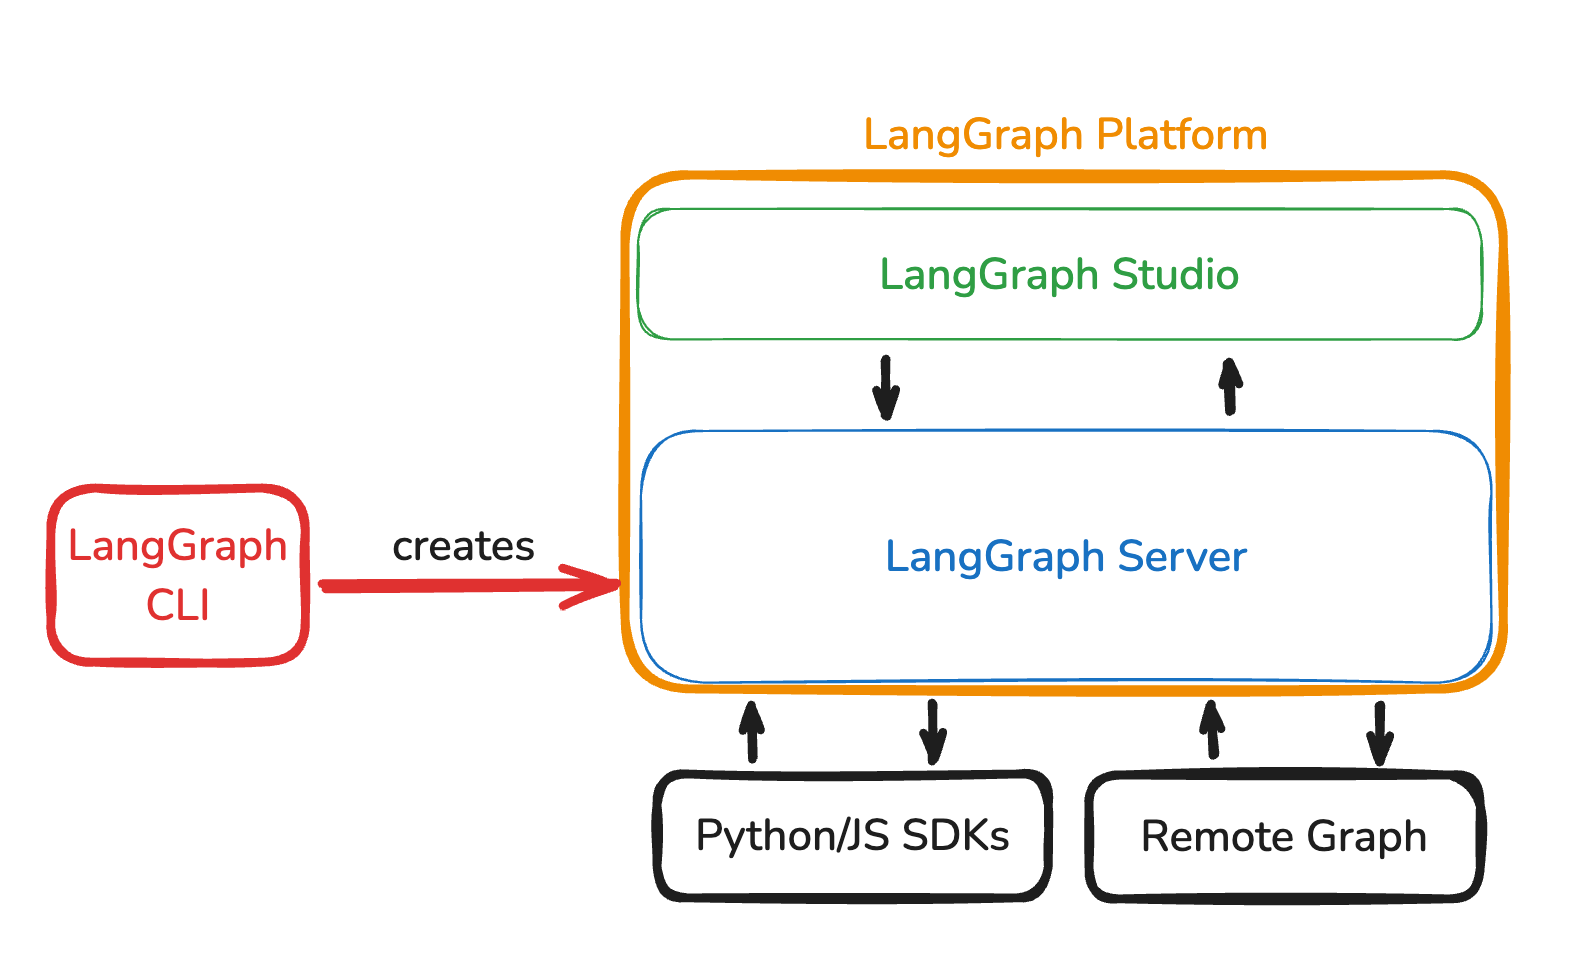
\includegraphics[width=0.8\textwidth]{bab2/langgraph_platform.png}
\caption[Arsitektur LangSmith Deployment]{Arsitektur LangSmith Deployment (sebelumnya LangGraph Platform) \parencite{langchainaiLangSmithSDK2025}}
\label{fig:langgraph_platform}
\end{figure}



\section{\textit{LLM-as-a-judge}}

\textit{LLM-as-a-judge} adalah pendekatan evaluasi yang memanfaatkan LLM untuk menilai keluaran LLM lainnya, sebagai respons atas tantangan dalam mengevaluasi respons yang bersifat \textit{open-ended} \parencite{huyenAIEngineeringBuilding2025}. Tantangan ini sebelumnya banyak diselesaikan dengan evaluasi manusia, yang tidak skalabel untuk kebutuhan produksi. Model yang berperan sebagai penilai disebut oleh \textcite{huyenAIEngineeringBuilding2025} sebagai \textit{AI judge}, sementara \textcite{oshinLearningLangchainBuilding2025} menyebutnya \textit{LLM-as-a-judge evaluators} atau sederhananya evaluator LLM. Secara umum, evaluator ini bekerja dengan mengintegrasikan aturan penilaian ke dalam \textit{prompt} LLM, yang kemudian menilai keluaran berdasarkan jawaban referensi yang tersedia \parencite{oshinLearningLangchainBuilding2025}. Dalam penerapannya, skor yang dihasilkan perlu diaudit dan evaluator perlu disetel secara iteratif agar penilaian yang dihasilkan dapat diandalkan.

Keunggulan utama dari metode ini terletak pada efisiensi biaya dan waktu dibandingkan dengan evaluasi manusia, serta kemampuannya untuk memberikan penilaian yang lebih bernuansa dibandingkan metrik heuristik. Sejumlah penelitian menunjukkan bahwa evaluator LLM memiliki korelasi yang tinggi dengan penilaian manusia. \textcite{zhengJudgingLLMasaJudgeMTBench2023} menemukan bahwa pada \textit{benchmark} MT-Bench, tingkat kesepakatan antara GPT-4 \parencite{openaiGPT4TechnicalReport2024} dan manusia mencapai 85\%, lebih tinggi dari kesepakatan antarmanusia yang sebesar 81\%. \textcite{duboisLengthControlledAlpacaEvalSimple2025} juga melaporkan bahwa evaluator LLM pada AlpacaEval memiliki korelasi hampir sempurna (0,98) dengan papan peringkat LMSYS Chat Arena yang dievaluasi secara manusia. 

Selain itu, evaluator LLM dapat menjelaskan alasan di balik penilaiannya, yang memudahkan proses audit hasil evaluasi \parencite{huyenAIEngineeringBuilding2025}. Fleksibilitas ini menjadikan \textit{LLM-as-a-judge} dapat diterapkan pada berbagai jenis aplikasi, bahkan menjadi satu-satunya opsi evaluasi otomatis untuk beberapa kasus penggunaan tertentu. Akan tetapi, \textcite{wangLargeLanguageModels2024} mengidentifikasi sejumlah tantangan, seperti bias posisi (\textit{positional bias}) di mana model cenderung memfavoritkan jawaban yang muncul pertama, serta bias kebertele-telean (\textit{verbosity bias}) yang memberikan skor lebih tinggi pada jawaban yang lebih panjang meskipun tidak lebih informatif.

Sebagai upaya untuk meningkatkan keselarasan dengan penilaian manusia, \textcite{liuGEvalNLGEvaluation2023} memperkenalkan kerangka kerja G-Eval. Pendekatan ini memanfaatkan teknik \textit{Chain-of-Thought} untuk mengarahkan LLM agar menghasilkan langkah-langkah penalaran evaluasi secara eksplisit sebelum memberikan skor akhir. Melalui proses penalaran bertahap ini, model dapat melakukan penilaian yang lebih terstruktur dan transparan, yang pada gilirannya meningkatkan akurasi evaluasi. Selain itu, adanya jejak penalaran memungkinkan verifikasi terhadap logika di balik setiap skor yang diberikan. Mekanisme kerja dari G-Eval ini diilustrasikan pada Gambar \ref{fig:geval_framework}.

\begin{figure}[H]
\centering
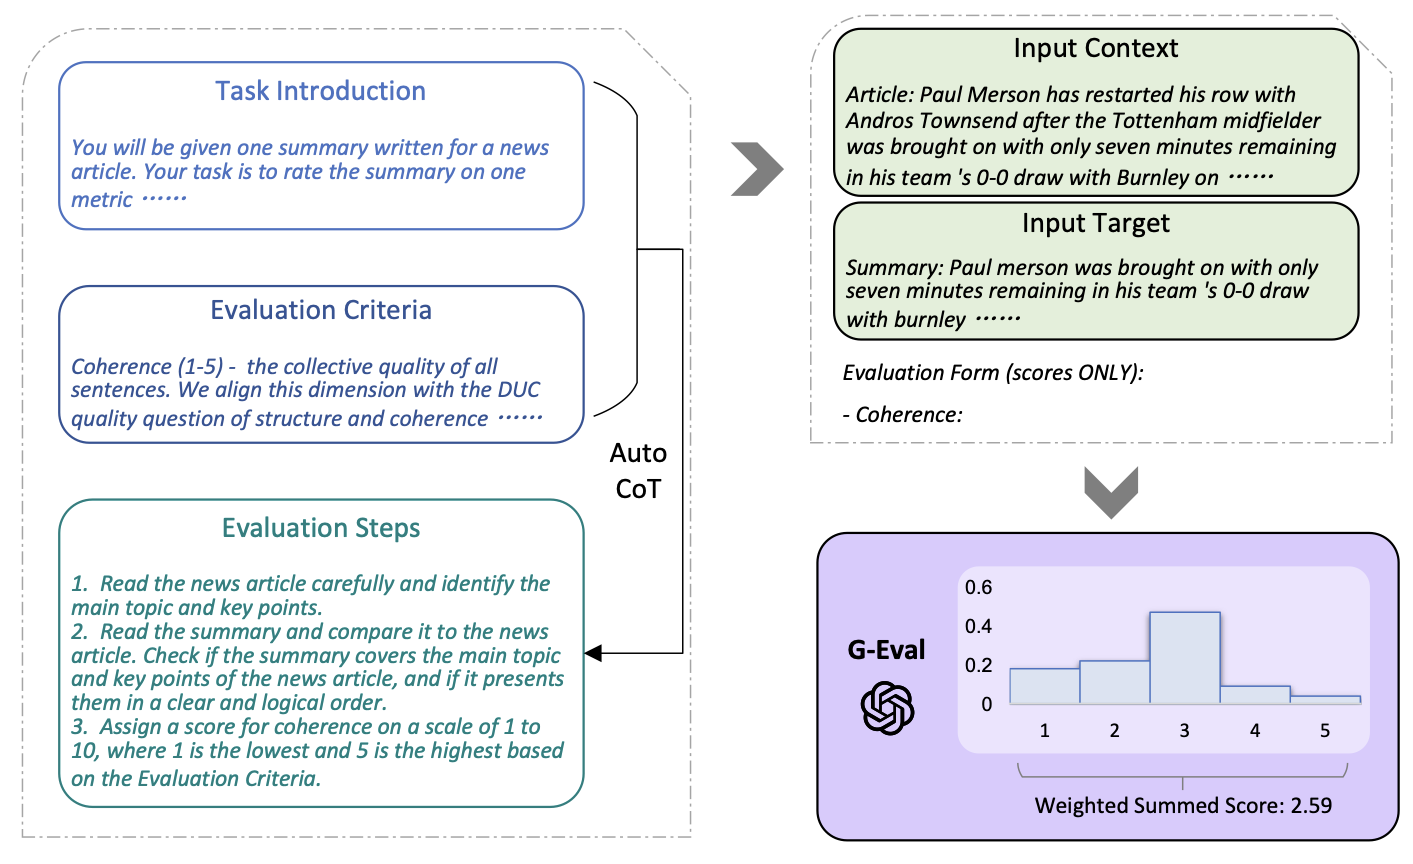
\includegraphics[width=0.65\textwidth]{bab2/kerangkakerjageval.png}
\caption[Kerangka kerja G-Eval]{Kerangka kerja G-Eval yang memanfaatkan \textit{Chain-of-Thought} untuk evaluasi \parencite{liuGEvalNLGEvaluation2023}}
\label{fig:geval_framework}
\end{figure}

Berdasarkan eksperimen yang dilakukan, G-Eval menunjukkan korelasi Spearman yang lebih tinggi dengan penilaian manusia dibandingkan dengan metode evaluasi otomatis sebelumnya, membuktikan bahwa penambahan langkah penalaran dapat meningkatkan reliabilitas LLM sebagai juri yang objektif. Hasil eksperimen pada \textit{benchmark} SummEval memperlihatkan bahwa G-Eval-4 mencatatkan kinerja unggul dengan rata-rata korelasi Spearman ($\rho$) sebesar 0,514 dan Kendall-Tau ($\tau$) sebesar 0,418. Capaian ini melampaui metrik konvensional seperti ROUGE-L yang hanya memperoleh rata-rata korelasi Spearman 0,165 dan Kendall-Tau 0,128, serta metrik berbasis model lainnya seperti BERTScore ($\rho=0,225$; $\tau=0,175$) dan UniEval ($\rho=0,474$; $\tau=0,377$). Dominasi G-Eval dalam metrik korelasi ini menegaskan bahwa pendekatan evaluasi berbasis LLM dengan penalaran mampu mendekati penilaian manusia secara lebih akurat dibandingkan metode-metode sebelumnya.

Walaupun gagasan penggunaan AI untuk mengotomasi evaluasi sudah ada sejak lama, pendekatan ini baru menjadi praktis seiring kemampuan model AI yang semakin memadai, yaitu sekitar saat GPT-3 dirilis oleh \textcite{brownLanguageModelsAre2020} \parencite{huyenAIEngineeringBuilding2025}. Sejak saat itu, \textit{LLM-as-a-judge} berkembang menjadi salah satu metode evaluasi yang paling umum digunakan dalam sistem AI produksi. \textcite{langchain_state_of_ai_2023} mencatat bahwa 58\% evaluasi pada platform LangChain dilakukan oleh \textit{AI judge}, mencerminkan adopsi yang luas di industri. Di samping itu, metode ini juga terus berkembang sebagai area penelitian yang aktif.

\subsection{Ragas (\textit{Retrieval Augmented Generation Assessment})}
Ragas (\textit{Retrieval Augmented Generation Assessment}) adalah kerangka kerja evaluasi otomatis yang dikembangkan oleh \textcite{esRagasAutomatedEvaluation2025} untuk mengukur kinerja sistem RAG, dan dapat diakses melalui \textit{library} Python dengan nama yang sama \parencite{ragas2024}. Kerangka kerja ini mengadopsi paradigma \textit{LLM-as-a-judge} dalam mengukur metrik untuk evaluasinya. Evaluasi dalam Ragas dilakukan secara \textit{reference-free} (tanpa referensi jawaban manusia) untuk sebagian metriknya, yang memungkinkan skalabilitas evaluasi pada dataset yang dinamis. Penilaian dilakukan terhadap tiga komponen utama dalam ekosistem RAG, yaitu pertanyaan (\textit{query}), konteks yang diambil (\textit{retrieved context}), dan jawaban yang dihasilkan (\textit{generated answer}). Ragas juga dirancang agar dapat diintegrasikan dengan berbagai \textit{framework} dan \textit{toolchain} yang berbeda seperti LangChain \parencite{langchainaiLangChain2025}, sehingga evaluasi dapat dilakukan tanpa harus mengganti tumpukan teknologi yang sudah digunakan.

\textcite{ragas2024} menyediakan sejumlah metrik evaluasi yang dikelompokkan berdasarkan tipe aplikasi, mencakup sistem RAG, \textit{workflow} agentik, dan perbandingan bahasa alami \parencite{ragas2024}. Untuk sistem RAG, dua metrik utama yang tersedia adalah \textit{Context Precision} dan \textit{Context Recall}, yang keduanya berfokus pada kualitas komponen \textit{retrieval}. \textit{Context Precision} mengukur sejauh mana potongan konteks yang relevan berada di peringkat atas dari konteks yang diambil, dihitung sebagai rata-rata \textit{precision@k} untuk setiap potongan. \textit{Context Recall} melengkapinya dengan mengukur proporsi klaim dalam jawaban referensi yang dapat diatribusikan ke konteks yang diambil, memastikan tidak ada informasi penting yang terlewat. Bersama-sama, kedua metrik ini mencerminkan kualitas \textit{retriever} dari dua sisi, yaitu ketepatan dan kelengkapan.

Untuk evaluasi \textit{workflow} agentik, \textcite{ragas2024} menyediakan beberapa metrik, di antaranya \textit{Tool Call Accuracy} dan \textit{Tool Call F1}. \textit{Tool Call Accuracy} mengukur keakuratan urutan dan argumen pemanggilan alat oleh agen terhadap referensi yang diharapkan, cocok digunakan saat urutan pemanggilan alat bersifat kritis. \textit{Tool Call F1} menawarkan pendekatan yang lebih longgar berbasis \textit{precision} dan \textit{recall} tanpa mempertimbangkan urutan, sehingga berguna untuk mengukur kedekatan perilaku agen dengan ekspektasi meskipun urutan panggilannya berbeda. Selain itu, tersedia pula metrik perbandingan bahasa alami seperti \textit{Factual Correctness} yang mengukur keakuratan faktual respons terhadap referensi melalui dekomposisi klaim dan \textit{natural language inference}, serta \textit{Semantic Similarity} yang mengukur kemiripan semantik antara respons dan referensi menggunakan \textit{embedding}.

\subsection{DeepEval}
DeepEval merupakan kerangka kerja evaluasi \textit{open-source} yang dirancang khusus untuk menguji dan mengevaluasi sistem berbasis LLM, seperti aplikasi RAG dan sistem agentik \parencite{confidentaiDeepEval2025}. Kerangka kerja ini menawarkan pendekatan yang modular dan mudah diintegrasikan dalam siklus pengembangan perangkat lunak serta mengadopsi prinsip pengujian unit (\textit{unit testing}) untuk memvalidasi luaran LLM secara sistematis. Hampir seluruh metrik bawaan DeepEval menggunakan paradigma \textit{LLM-as-a-judge} untuk menilai \textit{test case}, yakni satuan interaksi atomik pengguna dengan aplikasi LLM. DeepEval menyediakan berbagai metrik evaluasi yang sebagian besar memiliki dukungan riset dan seluruhnya bersifat \textit{multimodal} \parencite{confidentaiDeepEval2025}. Hal ini berarti metrik-metrik tersebut mendukung evaluasi sistem berbasis LLM yang memproses lebih dari sekadar teks, di mana \textit{test case} dapat memuat teks maupun citra sekaligus.

Salah satu metrik yang didukung DeepEval adalah implementasi G-Eval dari \textcite{liuGEvalNLGEvaluation2023}, yang menggunakan \textit{CoT prompting} untuk menstabilkan komputasi skor dan membuat penilaian LLM judge lebih andal dan konsisten. Walaupun efektif untuk tugas yang memerlukan penilaian subjektif seperti koherensi dan relevansi jawaban, menurut \textcite{confidentaiDeepEval2025}, G-Eval masih bersifat non-deterministik, sehingga hasil evaluasi dapat bervariasi antar eksekusi pada masukan yang sama. Keterbatasan ini menjadi kendala saat kriteria evaluasi bersifat eksplisit dan terstruktur, seperti pada kebutuhan verifikasi format luaran. 

Untuk mengatasi hal tersebut, DeepEval juga mengembangkan metrik berbasis \textit{Directed Acyclic Graph} (DAG) sebagai alternatif yang lebih deterministik \parencite{confidentaiDeepEval2025}. Dalam pendekatan ini, setiap simpul merepresentasikan LLM judge yang menangani satu keputusan spesifik, sedangkan sisi-sisinya mendefinisikan alur logis antar keputusan. Dengan memecah proses evaluasi menjadi unit-unit atomik yang lebih kecil, ambiguitas diminimalkan sehingga keselarasan dengan ekspektasi dapat ditegakkan secara lebih ketat, seperti yang diilustrasikan pada Gambar~\ref{fig:dag_contoh}.

\begin{figure}[H]
\centering
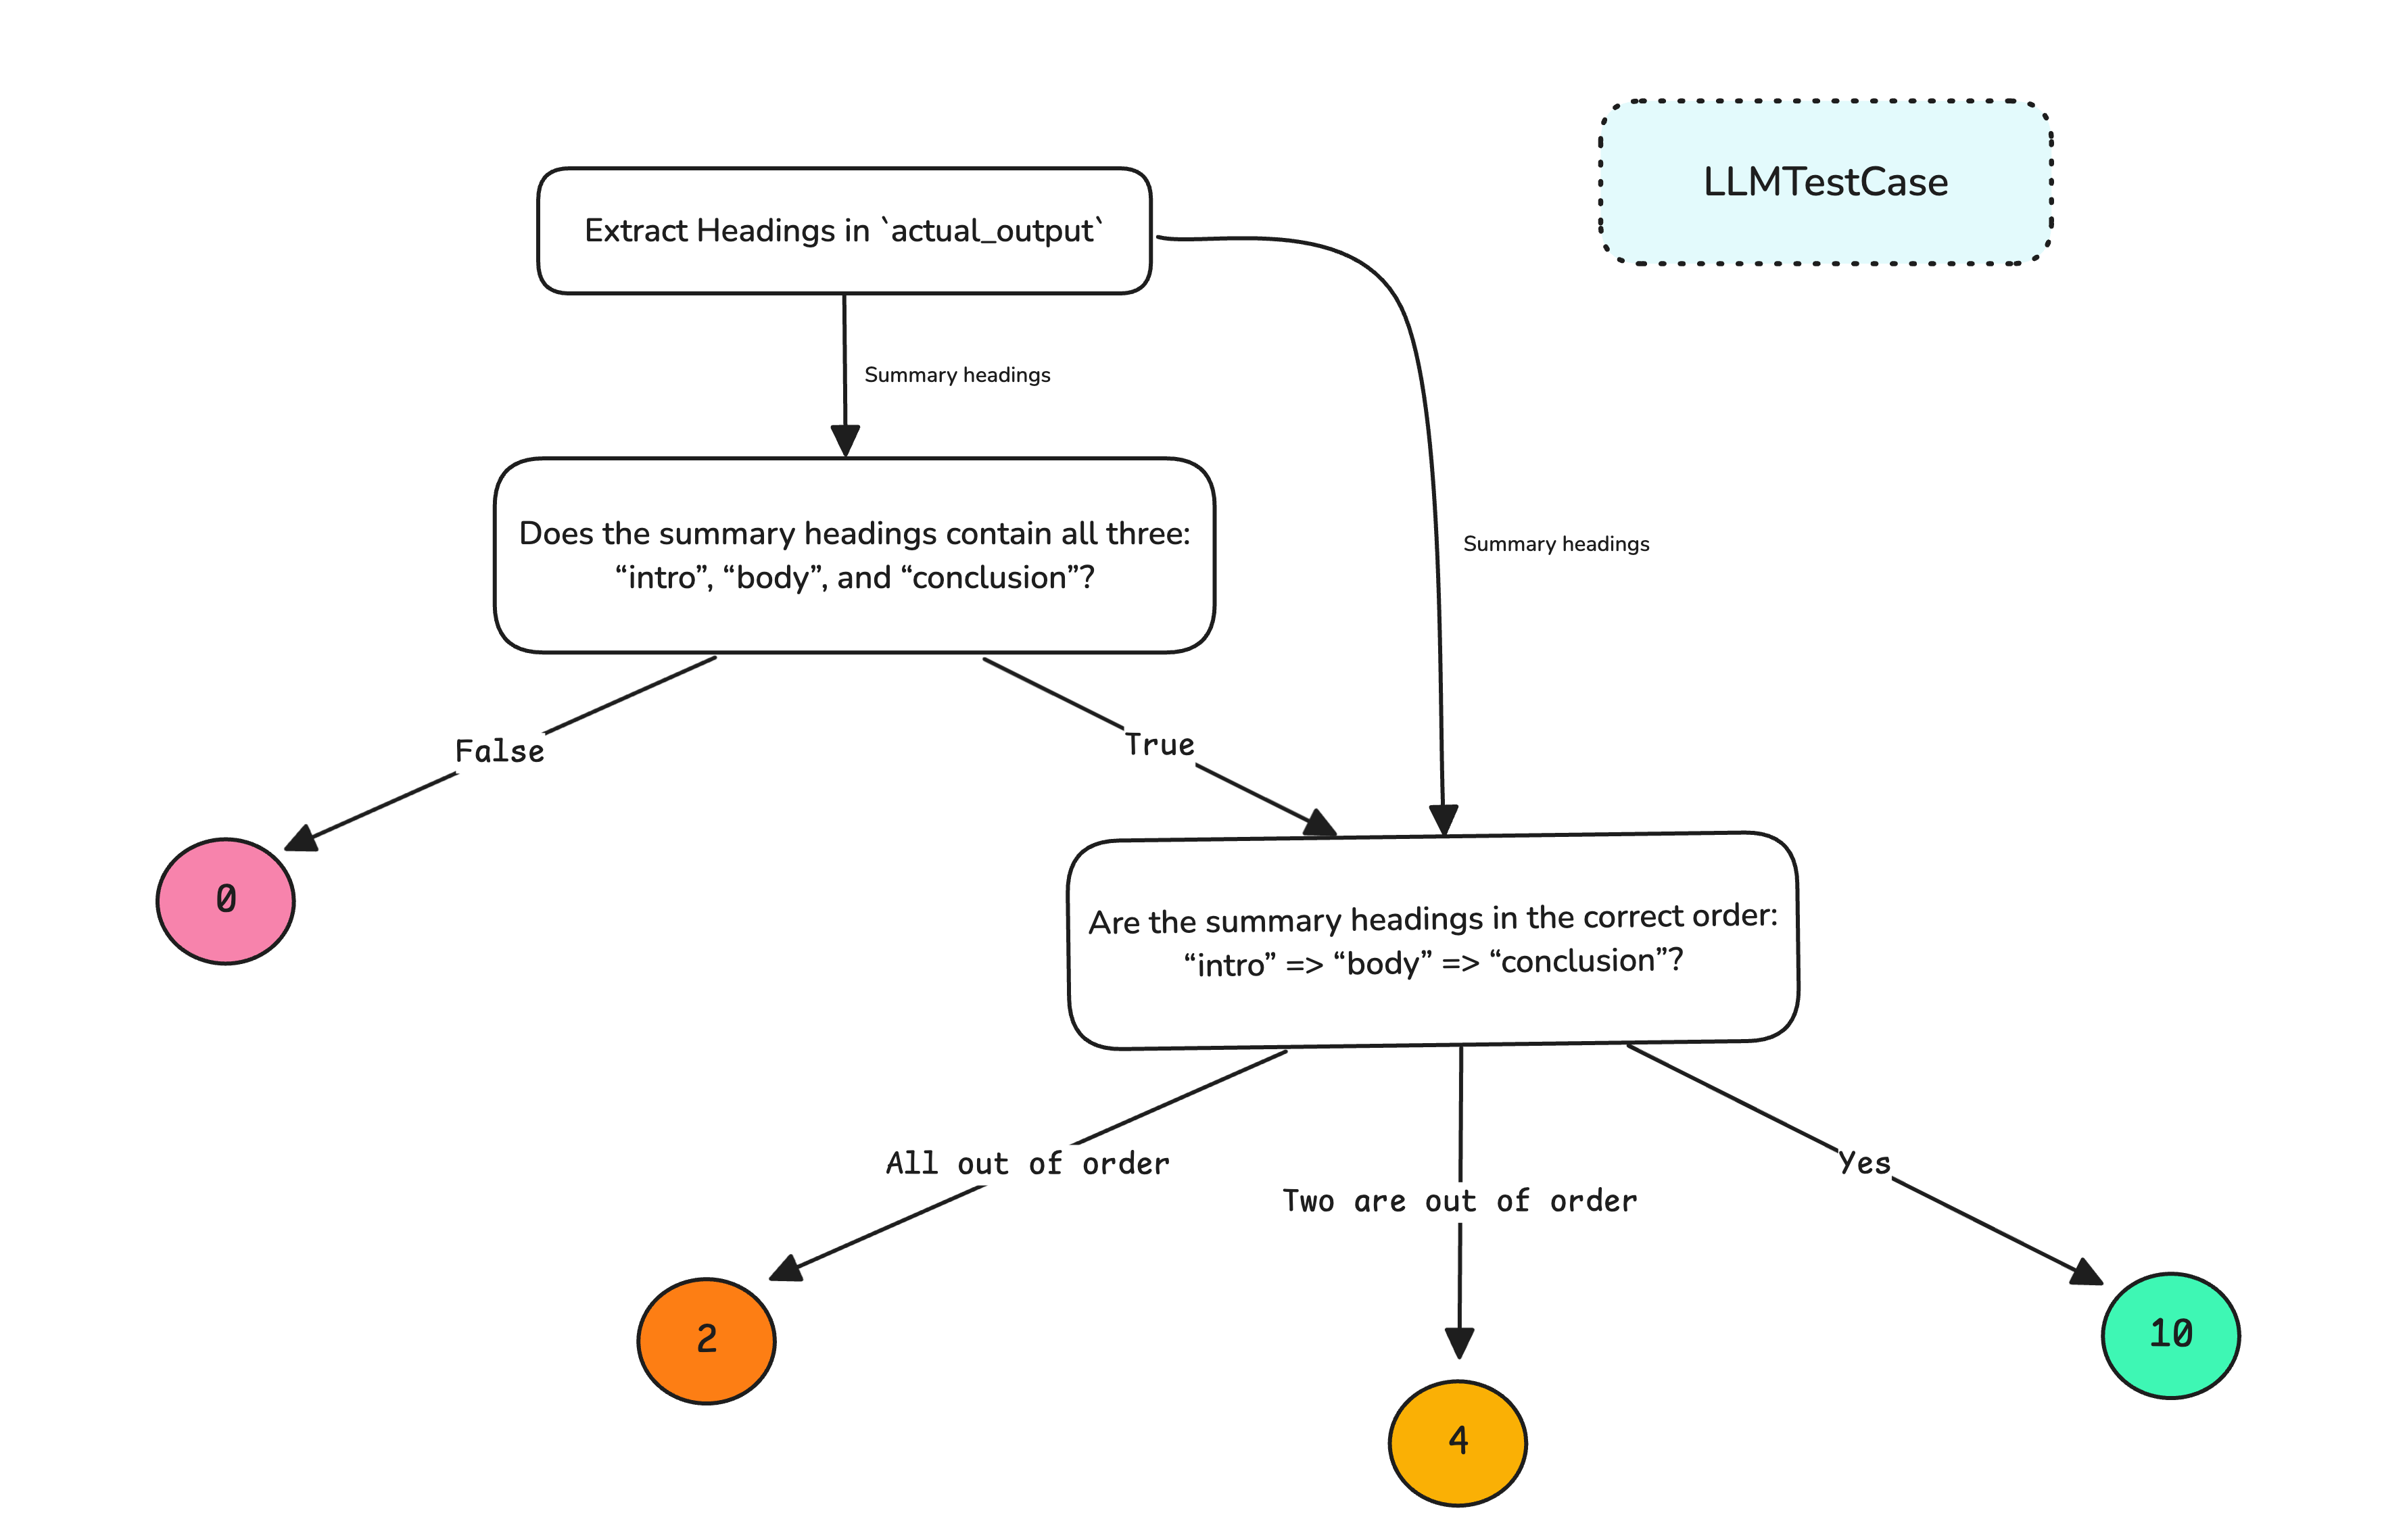
\includegraphics[width=0.75\textwidth]{bab2/contoh_dag.png}
\caption[Contoh arsitektur metrik DAG pada DeepEval]{Contoh arsitektur metrik DAG pada DeepEval yang mengevaluasi \textit{actual output} melalui serangkaian keputusan atomik yang terstruktur \parencite{confidentaiDeepEval2025}}
\label{fig:dag_contoh}
\end{figure}

\section{Penelitian Terkait}
Pada penelitian terkait, berbagai pendekatan sistem agentik dengan beberapa ragam augmentasi LLM dan integrasi model \textit{deep learning} hingga \textit{computer vision} telah digunakan untuk tugas yang berkaitan dengan identifikasi penyakit tanaman. Pada implementasi paling sederhana, \textcite{sbDesignImplementationAIPowered2024} mengembangkan sistem agentik untuk deteksi penyakit tanaman sekaligus memberikan rekomendasi penanganan. Sistem ini memanfaatkan YOLOv5 untuk mengidentifikasi daun tanaman yang terinfeksi pada berbagai spesies dan jenis penyakit. Selanjutnya, sistem diintegrasikan dengan LLM dari Gemini API guna menyediakan rekomendasi penanganan yang disesuaikan dengan jenis penyakit yang terdeteksi. Evaluasi sistem hanya dilakukan pada model YOLOv5 yakni dengan \textit{mean Average Precision} (mAP) sebesar 0,85 dan \textit{precision} sebesar 0,88 dalam diagnosis penyakit. Pendekatan dari sistem agentik ini dapat dikatakan sebagai \textit{workflow} tanpa ada teknik augmentasi dari LLM, sehingga beresiko terjadi halusinasi.

Mengembangkan dari pendekatan sebelumnya, \textcite{mondalVisionMeetsLanguage2025} memperkenalkan sistem yang lebih maju dengan menggabungkan YOLO dan RAG untuk augmentasi LLM. Sistem ini memanfaatkan YOLOv8 untuk terlebih dahulu mendeteksi penyakit pada daun kopi, kemudian mengintegrasikan mekanisme RAG untuk memberikan hasil diagnosis yang relevan. Pengujian dan evaluasi hanya dilakukan pada model YOLOv8 yang mendapatkan mAP@0.5 sebesar 0.681 dalam deteksi. Sistem agentik ini sendiri merupakan pendekatan \textit{workflow} dengan teknik augmentasi tambahan untuk LLM melalui RAG.

Alternatif pendekatan lainnya terdapat pada penelitian \textcite{roumeliotisPlantDiseaseDetection2025} yang mengeksplorasi penggunaan GPT-4o sebagai LLM \textit{multimodal} dan digabungkan dengan ResNet-50 untuk klasifikasi penyakit tanaman dari citra daun. \citeauthor{roumeliotisPlantDiseaseDetection2025} melakukan evaluasi dalam \textit{setting zero-shot}, \textit{few-shot}, dan \textit{progressive fine-tuning} menggunakan \textit{dataset} PlantVillage, pada dua spesies tanaman, yaitu apel dan jagung, dengan gambar resolusi 100, 150, dan 256 piksel. Hasilnya menunjukkan bahwa model GPT-4o yang di-\textit{fine-tune} mencapai akurasi tertinggi sekitar 98,12\% pada citra daun apel 256 px, sedikit lebih baik dibanding ResNet-50 di $\sim$96,88\% pada kondisi yang sama. Namun, performa \textit{zero-shot} GPT-4o, menunjukkan bahwa meski model \textit{multimodal} LLM kuat, pelatihan tetap diperlukan. Selain itu, meskipun model menunjukkan adaptasi yang baik terhadap berbagai resolusi gambar, generalisasi ke spesies tanaman yang berbeda tetap memiliki batasan, khususnya ketika struktur daun cukup berbeda. Secara keseluruhan, penelitian ini menunjukkan penerapan \textit{workflow} dengan augmentasi \textit{fine-tuning} pada LLM.

Pendekatan yang menarik terdapat pada penelitian \textcite{xuMultimodalAgriculturalAgent2025} yang mengusulkan MA3 sebagai pendekatan \textit{workflow} yang dapat mengambil keputusan dalam identifikasi penyakit tanaman secara adaptif. Arsitektur ini dirancang agar lebih adaptif melalui modul \textit{router} berisi model BERT yang dilatih secara \textit{supervised learning} untuk mengklasifikasikan \textit{query} (\textit{input} teks) pengguna. Berdasarkan hasil klasifikasi tersebut, sistem dapat mengarahkan proses ke modul klasifikasi penyakit, deteksi penyakit, atau tanya jawab. Modul klasifikasi dan deteksi dibangun menggunakan \textit{backbone} CLIP-ViT yang di-\textit{fine-tune} untuk data penyakit tebu, sementara komponen terakhir memanfaatkan Qwen2.5-32B sebagai LLM guna menggabungkan keluaran seluruh alat dan menyusun jawaban akhir yang lebih informatif. Integrasi komponen-komponen ini menjadikan MA3 sebagai sistem yang \textit{multimodal}, karena sistem mampu memproses masukan berupa teks sekaligus citra, di mana teks diproses oleh \textit{router} dan LLM, sementara citra diproses oleh modul berbasis CLIP-ViT untuk klasifikasi maupun deteksi penyakit.

Dengan desain MA3, \textcite{xuMultimodalAgriculturalAgent2025} menghadirkan pendekatan \textit{workflow} adaptif yang membedakannya dari pendekatan agen, karena pemilihan alat dikendalikan oleh \textit{router}, bukan oleh LLM itu sendiri. Pilihan penggunaan \textit{router} dalam penggunaan alat yang adaptif dimaksudkan untuk menghindari halusinasi dari LLM. Akan tetapi \citeauthor{xuMultimodalAgriculturalAgent2025} luput menyebutkan pendekatan seperti agen dengan pola ReAct yang sebenarnya sudah menawarkan solusi atas masalah tersebut. Di mana, pola ReAct dapat diterapkan langsung ke LLM untuk memberikan kemampuan pengambilan keputusan yang adaptif dalam memilih alat, tanpa perlu menambahkan komponen \textit{router} terpisah. 

Hasil evaluasi pada sistem yang dikembangkan penelitian \textcite{xuMultimodalAgriculturalAgent2025} menunjukkan bahwa \textit{router} BERT mencapai akurasi sangat tinggi di atas 99\%, modul klasifikasi penyakit memperoleh \textit{precision} hingga 96,2\%, sedangkan modul deteksi penyakit masih menghadapi tantangan dengan mAP sekitar 0,325. Evaluasi dilakukan dengan kombinasi metrik tradisional serta metrik kualitas tanya jawab seperti \textit{semantic consistency}, \textit{information completeness}, \textit{information leakage}, dan \textit{redundancy} oleh \textit{evaluator} pakar di bidang pertanian secara \textit{offline}. Pada sistem agentik yang dikembangkan, \textcite{xuMultimodalAgriculturalAgent2025} juga memperkenalkan metode evaluasi \textit{online} menggunakan LLM berupa DeepSeek-V3 sebagai evaluator LLM untuk memeriksa kualitas dan relevansi dari penggunaan berbagai komponen MA3, baik dalam tugas klasifikasi, deteksi, maupun tanya jawab.

Sejauh ini belum ada penelitian yang menerapkan pendekatan agen dalam sistem agentik untuk identifikasi penyakit tanaman melalui pola ReAct, maupun mengintegrasikannya dengan VLM dan dapat mengevaluasi sistemnya secara komprehensif. Pendekatan yang paling mendekati ditunjukkan oleh ShizishanGPT yang diperkenalkan oleh \textcite{yangShizishanGPTAgriculturalLarge2024}, yakni sebuah sistem agentik yang dirancang untuk mendukung berbagai tugas agrikultur, termasuk seputar penyakit tanaman, meski penggunaannya masih terbatas pada skenario tanya jawab tanpa analisis citra. Dalam sistem, terdapat agen LLM dengan pola ReAct yang menggunakan GPT-4 dengan akses modul yang berisi alat eksternal seperti pencarian internet, prediksi fenotipe tanaman, analisis gen, dan model cuaca. ShizishanGPT juga memiliki modul pengambilan informasi berbasis RAG, tetapi modul ini tidak terintegrasi pada agen sebagai alat, sehingga penggunaannya tidak adaptif. 

Untuk eksperimen, \textcite{yangShizishanGPTAgriculturalLarge2024} menyiapkan \textit{dataset} sintetis berisi 100 pasangan pertanyaan dan jawaban pertanian yang digenerasi oleh LLM. Evaluasi dilakukan melalui \textit{machine scoring} pada modul pengambilan informasi berbasis RAG menggunakan beberapa metrik, di mana ShizishanGPT meraih skor komposit tertinggi di 0,923. Selain itu, \textit{manual scoring} oleh \textit{evaluator} untuk akurasi, profesionalisme, dan kemampuan bahasa dari jawaban menempatkan ShizishanGPT pada skor 9,65 dari 10, lebih unggul dibanding GPT-4 maupun model lainnya. Evaluasi juga dilakukan melalui eksperimen yang menghapus beberapa modul dari sistem untuk menilai kontribusi masing-masing komponen. Hasilnya menunjukkan konfigurasi penuh memberikan hasil terbaik, sementara penghapusan modul pengambilan informasi berbasis RAG memberikan skor terendah di 9,21, menunjukkan peran penting RAG dalam menjaga kualitas jawaban. 

Secara keseluruhan, penelitian-penelitian sebelumnya menunjukkan berbagai pendekatan dalam penerapan sistem agentik untuk identifikasi penyakit tanaman. Penerapan ini dimulai dari integrasi \textit{workflow} sederhana dengan YOLO dan LLM, pengambilan informasi melalui RAG, \textit{fine-tuning} pada LLM, hingga arsitektur \textit{workflow} yang kompleks dengan \textit{router} dan model-model khusus. Peningkatan signifikan terlihat pada \textcite{xuMultimodalAgriculturalAgent2025} dengan munculnya sistem agentik yang lebih otonom dan reliabel. Akan tetapi, belum ada yang secara komprehensif mengintegrasikan pola ReAct dengan VLM untuk identifikasi penyakit tanaman secara \textit{end-to-end} dengan evaluasi yang menyeluruh. Rangkuman dari penelitian-penelitian tersebut ditunjukkan pada Tabel \ref{tab:summary_related_research}. Rangkuman ini disusun dengan menyoroti aspek pendekatan sistem agentik yang digunakan, augmentasi LLM, integrasi model atau teknologi tambahan, serta hasil evaluasi utama yang dilaporkan dalam setiap penelitian.

{
\setstretch{1.0}
\begin{longtblr}[
    caption = {Rangkuman penelitian terkait sistem agentik untuk identifikasi penyakit tanaman},
    entry = {Rangkuman penelitian terkait},
    label = {tab:summary_related_research},
]{
    width = \linewidth,
    colspec = {X[1.5,l] X[2,l] X[2,l] X[2,l]},
    rows = {m},
    rowhead = 1,
    row{1} = {font=\bfseries, halign=c, valign=m},
    hlines, vlines,
    rowsep = 3pt,
}
    Peneliti dan Tahun & Pendekatan Sistem Agentik & Integrasi Tambahan & Evaluasi \\
    \textcite{sbDesignImplementationAIPowered2024} & \textit{Workflow} sederhana & YOLOv5 untuk deteksi penyakit tanaman & mAP 0,85 dan \textit{precision} 0,88 pada model YOLOv5 \\
    \textcite{roumeliotisPlantDiseaseDetection2025} & \textit{Workflow} sederhana dengan \textit{fine-tuning} LLM & ResNet-50 untuk klasifikasi tanaman & Akurasi hingga 98,12\% pada GPT-4o (\textit{fine-tuned}) dan $\sim$96,88\% pada ResNet-50 \\
    \textcite{xuMultimodalAgriculturalAgent2025} & \textit{Workflow} adaptif dengan \textit{fine-tuning} LLM & BERT sebagai \textit{router} penggunaan alat adaptif dan CLIP-ViT untuk deteksi lesi serta klasifikasi penyakit tanaman & \textit{Router} akurasi $>$99\%; klasifikasi \textit{precision} 96,2\%; deteksi mAP $\sim$0,325; Evaluasi komponen menggunakan \textit{LLM-as-a-judge} \\
    \textcite{yangShizishanGPTAgriculturalLarge2024} & Kombinasi \textit{workflow} dengan ReAct & RAG, model--model untuk berbagai tugas, dan pencarian internet & Skor komposit RAG 0,923 (\textit{machine scoring}) dan skor manual 9,65/10 (\textit{human scoring}) \\
\end{longtblr}
}


\chapter{METODE PENELITIAN}

\section{Desain Penelitian}
Penelitian ini dilakukan dengan mengadopsi metode \textit{Design and Development} (D\&D) yang dirumuskan oleh \textcite{ellisGuideNoviceResearchers2010}. Metode D\&D didefinisikan sebagai pendekatan sistematis untuk merancang, mengembangkan, dan mengevaluasi suatu produk atau sistem (artefak) sebagai solusi atas permasalahan yang spesifik. Berbeda dengan metode penelitian tradisional yang umumnya berfokus pada pengujian hipotesis atau observasi fenomena, penelitian D\&D menempatkan pengembangan artefak teknologi itu sendiri sebagai kontribusi utama terhadap khazanah pengetahuan. Tujuan utamanya adalah untuk menjembatani kesenjangan antara landasan teoritis dan implementasi praktis melalui penciptaan solusi yang dapat diuji validitas dan efektivitasnya.

Metode ini dipilih karena kesesuaiannya dengan karakteristik penelitian ini yang berfokus pada pengembangan prototipe sistem agentik. Menurut \textcite{ellisGuideNoviceResearchers2010}, pendekatan D\&D menyediakan kerangka kerja yang terstruktur untuk memandu proses teknis mulai dari konseptualisasi hingga validasi sistem. Hal ini dinilai relevan mengingat luaran penelitian masih terbatas dalam bentuk prototipe yang berhenti pada tahap validasi fungsional dan kinerja, sehingga diperlukan metodologi yang menekankan pada iterasi desain dan pembuktian konsep (\textit{proof of concept}). Tahapan pelaksanaan penelitian mengacu pada enam fase dalam model D\&D, yaitu identifikasi masalah, deskripsi tujuan, perancangan dan pengembangan, pengujian, evaluasi, dan penyampaian hasil. Alur tahapan tersebut divisualisasikan pada Gambar \ref{fig:dnd}.

\begin{figure}[H] 
    \centering
    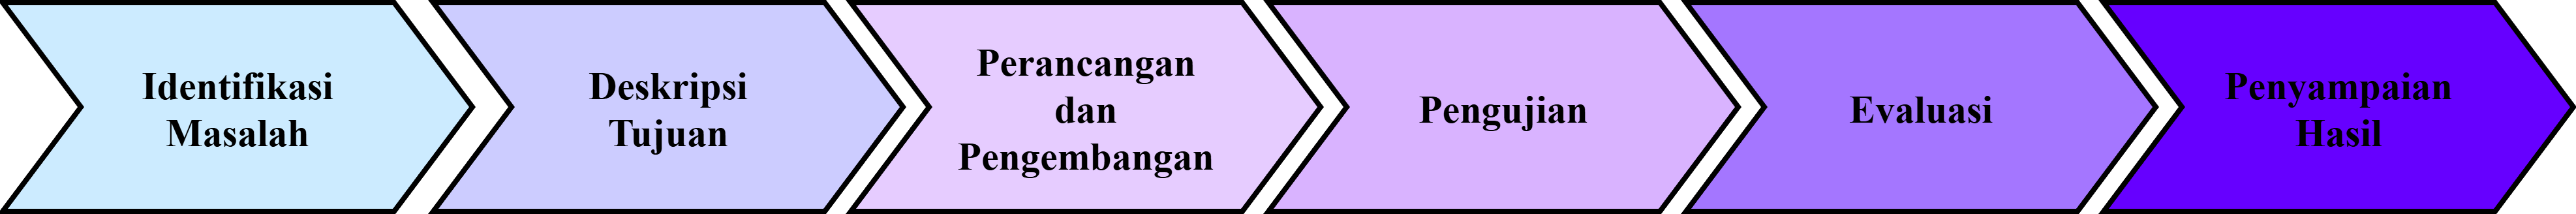
\includegraphics[width=1\textwidth]{bab3/dnd.png}
    \caption[Tahapan penelitian metode \textit{Design and Development} (D\&D)]{Tahapan penelitian metode \textit{Design and Development} (D\&D) \parencite{ellisGuideNoviceResearchers2010}}
    \label{fig:dnd}
\end{figure}

\section{Identifikasi Masalah}


% \begin{table}[H]
%     \centering
%     \caption{Perangkat Pendukung Penelitian}
%     \label{tab:perangkat_pendukung}
%     \small
%     \setstretch{1.0}
%     \begin{tabular}{|c|l|p{9cm}|}
%     \hline
%     \multicolumn{3}{|c|}{\textbf{Spesifikasi Laptop}} \\ \hline
%     \textbf{No.} & \textbf{Komponen} & \textbf{Spesifikasi} \\ \hline
%     1. & Prosesor & AMD Ryzen™ 7 7840HS \\ \hline
%     2. & Memori & 16 GB DDR5-5600 \\ \hline
%     3. & Grafik & NVIDIA® GeForce RTX™ 4060 8GB \\ \hline
%     \multicolumn{3}{|c|}{\textbf{Perangkat Lunak}} \\ \hline
%     \textbf{No.} & \textbf{Nama} & \textbf{Fungsi} \\ \hline
%     1. & WSL2 & Subsistem Linux untuk Windows sebagai lingkungan pengembangan sistem agentik. \\ \hline
%     2. & Docker & Platform kontainerisasi aplikasi. \\ \hline
%     3. & uv & Manajer library dan virtual environtment untuk Python. \\ \hline
%     4. & Next.js & Framework aplikasi web. \\ \hline
%     5. & LangChain & Framework pengembangan aplikasi LLM. \\ \hline
%     6. & LangGraph & Framework untuk pengembangan sistem agentik. \\ \hline
%     7. & LangSmith & Platform monitoring dan evaluasi LLM. \\ \hline
%     8. & AgentEval & Library evaluasi sistem agentik dari LangSmith. \\ \hline
%     9. & DeepEval & Library penyedia metrik evaluasi LLM-as-a-judge untuk sistem agentik. \\ \hline
%     10. & RAGAS & Library penyedia metrik evaluasi LLM-as-a-judge untuk RAG. \\ \hline
%     11. & Qdrant & Basis data vektor untuk pencarian semantik. \\ \hline
%     12. & Google Gen AI & Layanan penyedia API model bahasa Gemini. \\ \hline
%     13. & Voyage AI & Layanan penyedia API model embedding dan reranker. \\ \hline
%     14. & Kaggle Kernel & Platform komputasi untuk pelatihan model. \\ \hline
%     15. & Supabase & Layanan penyedia penyimpanan data. \\ \hline
%     16. & Cloudflare R2 & Layanan penyedia penyimpanan objek. \\ \hline
%     17. & FastEmbed & Library inferensi model embedding untuk RAG. \\ \hline
%     18. & LlamaIndex & Framework untuk pengembangan RAG. \\ \hline
%     19. & Playwright & Framework untuk automasi web untuk \textit{crawling}. \\ \hline
%     20. & ScrapeGraphAI & Library untuk ekstraksi data web berbasis LLM. \\ \hline
%     21. & Google Cloud Run & Layanan deployment cloud container . \\ \hline
%     22. & Vercel & Layanan hosting aplikasi web. \\ \hline
%     \end{tabular}
% \end{table}

\section{Deskripsi Tujuan}
Berdasarkan identifikasi masalah yang telah diuraikan, tujuan utama dari penelitian ini adalah mengembangkan sistem agentik multimodal yang mampu mengidentifikasi penyakit tanaman serta memberikan penjelasan diagnosis yang berbasis bukti. Sistem ini dirancang sebagai solusi untuk mengatasi keterbatasan metode identifikasi konvensional yang kurang adaptif. Secara rinci, tujuan pengembangan dalam penelitian ini dijabarkan sebagai berikut:
\begin{enumerate}[nosep]
    \item Mengembangkan arsitektur sistem agentik menggunakan pola \textit{Reasoning and Acting} (ReAct) yang memungkinkan model bahasa besar untuk memilih dan menggunakan alat bantu secara adaptif dalam proses diagnosis.
    \item Mengintegrasikan model deteksi objek YOLOv11 dan OWLv2 untuk melokalisasi gejala penyakit pada bagian tanaman secara spesifik.
    \item Mengimplementasikan modul pencarian multimodal berbasis model SCOLD untuk memungkinkan identifikasi penyakit melalui pencarian kemiripan visual dan tekstual pada basis data vektor.
    \item Menerapkan mekanisme \textit{Retrieval-Augmented Generation} (RAG) untuk memperkaya respon sistem dengan informasi manajemen penyakit yang faktual dari sumber pengetahuan eksternal.
    \item Merancang antarmuka pengguna berbasis web yang memfasilitasi interaksi dua arah antara pengguna dan sistem melalui teks dan gambar.
    \item Mengevaluasi kinerja sistem agentik yang dikembangkan menggunakan pendekatan \textit{LLM-as-a-judge} untuk mengukur akurasi diagnosis dan relevansi saran yang diberikan.
\end{enumerate}

\section{Perancangan dan Pengembangan}
Tahap perancangan dan pengembangan difokuskan pada realisasi teknis dari sistem agentik yang diusulkan. Pada bagian ini, arsitektur sistem dan implementasi komponen-komponen utamanya dijabarkan secara rinci. Pembahasan diawali dengan perancangan sistem agentik yang mengadopsi pola ReAct dan pengembangan agen LLM yang berfungsi sebagai pengendali logika sistem. Selanjutnya, uraian dilanjutkan pada pengembangan modul-modul spesifik yang mendukung kapabilitas sistem, meliputi modul deteksi objek tanaman, modul pencarian multimodal gambar-teks, serta modul pencarian informasi. Akhirnya, pengembangan antarmuka pengguna dipaparkan sebagai komponen interaksi antara pengguna dan sistem yang telah dibangun.

\subsection{Sistem Agentik}
Sistem agentik dalam penelitian ini dirancang dengan mengadopsi pola \textit{Reasoning and Acting} (ReAct). Implementasi sistem dilakukan menggunakan framework LangChain melalui library LangGraph \parencite{langchainaiLangChain2025}. Arsitektur sistem yang dikembangkan bersifat multimodal, di mana agen mampu menerima dan memproses input berupa citra tanaman serta instruksi tekstual dari pengguna secara bersamaan. Gambar \ref{fig:arsitektur_sistem_agentik} menyajikan arsitektur sistem agentik beserta spesifikasi input dan output pada setiap alat yang terintegrasi.

\begin{figure}[H]
    \centering
    \includegraphics[width=1\textwidth]{bab3/arsitektursistemagentik.png}
    \caption{Arsitektur sistem agentik dengan kemampuan multimodal}
    \label{fig:arsitektur_sistem_agentik}
\end{figure}

Dalam implementasi teknis menggunakan LangGraph, konsep teoritis ReAct yang diajukan oleh \textcite{yaoReActSynergizingReasoning2023} diterjemahkan ke dalam struktur graf berstatus (\textit{stateful graph}). Pada desain aslinya, pola ReAct diimplementasikan secara linier melalui teknik \textit{prompting}, di mana LLM menghasilkan teks terstruktur berisi penalaran (\textit{thought}) dan tindakan (\textit{action}) yang kemudian diurai oleh lingkungan eksternal. Di lain sisi, LangGraph memodelkan agen sebagai sistem yang terdiri dari \textit{node} (simpul) dan \textit{edge} (sisi). 

Struktur ini memetakan siklus Thought-Action-Observation ke dalam dua komponen utama, yaitu \textit{node} Model yang berisi agen dan \textit{node} Tools yang berisi alat. \textit{node} Model bertanggung jawab untuk menentukan apakah suatu tugas memerlukan penggunaan alat berdasarkan konteks yang diberikan. Jika alat diperlukan, LLM akan menghasilkan permintaan pemanggilan alat (\textit{tool call}) yang valid secara skema untuk dieksekusi secara otomatis oleh \textit{node} Tools. Hasil eksekusi tersebut dikembalikan ke \textit{node} Model sebagai observasi untuk dianalisis lebih lanjut hingga solusi akhir tercapai. 

Status (\textit{state}) agen dikelola sebagai objek yang menyimpan riwayat pesan, yang berfungsi sebagai memori jangka pendek atau \textit{scratchpad}. Alur kerja dimulai dari \textit{node} Model, di mana LLM memproses input dan menentukan langkah selanjutnya. Jika model memutuskan untuk menggunakan alat, alur dialihkan melalui \textit{conditional edge} menuju \textit{node} Tools. Setelah alat dieksekusi, hasilnya dicatat ke dalam state sebagai observasi, dan kendali dikembalikan ke \textit{node} Model untuk mengevaluasi informasi baru tersebut. Proses iteratif ini berlanjut hingga model menilai bahwa informasi yang dikumpulkan telah memadai untuk memberikan jawaban akhir (END). Visualisasi perbandingan antara desain teoritis ReAct dengan implementasi berbasis graf pada LangGraph disajikan pada Gambar \ref{fig:react_langgraph_comparison}.

\begin{figure}[H]
    \centering
    \includegraphics[width=1\textwidth]{bab3/reactlanggraph.png}
    \caption[Perbandingan antara (a) desain teoritis ReAct dan (b) implementasi berbasis graf pada LangGraph]{Perbandingan antara (a) desain teoritis ReAct oleh \textcite{yaoReActSynergizingReasoning2023} dan (b) implementasi berbasis graf pada LangGraph}
    \label{fig:react_langgraph_comparison}
\end{figure}

\subsection{Agen LLM}
Bagian ini menjelaskan spesifikasi dan konfigurasi agen LLM yang dikembangkan untuk mengimplementasikan pola ReAct pada sistem identifikasi penyakit tanaman.

\subsubsection{Konfigurasi}
Agen dalam penelitian ini digerakkan oleh Gemini 3 Flash sebagai LLM utama. Pemilihan model ini didasarkan pada karakteristik model yang menawarkan kecepatan inferensi tinggi dan kemampuan penalaran (\textit{reasoning}) serta penggunaan alat (\textit{tool-use}) yang sangat baik untuk tugas-tugas agentik. Konfigurasi model diatur dengan nilai \textit{temperature} 0 guna memastikan luaran yang bersifat deterministik dan konsisten, sehingga meminimalkan variasi jawaban yang tidak relevan dalam konteks teknis identifikasi penyakit.

Melalui implementasi arsitektur LangGraph, agen memiliki memori jangka pendek (\textit{short-term memory}) yang dikelola melalui objek \textit{State} (status) yang bersifat \textit{stateful}. Status ini berfungsi sebagai buku catatan (\textit{scratchpad}) yang menyimpan seluruh riwayat interaksi dan informasi yang dikumpulkan selama satu sesi tugas berlangsung. Dengan menyimpan status secara terstruktur, agen memiliki konteks terhadap langkah-langkah yang telah diambil sebelumnya, misalnya hasil deteksi objek atau temuan dari pencarian internet, yang kemudian digunakan sebagai dasar untuk menentukan langkah tindakan selanjutnya hingga solusi akhir tercapai. Tabel \ref{tab:state_components} menyajikan rincian variabel status yang dikelola dalam sistem.

\begin{table}[H]
    \centering
    \caption{Komponen Status (\textit{State}) pada Agen LLM}
    \label{tab:state_components}
    \small
    \setstretch{1.0}
    \begin{tabular}{|l|l|p{4cm}|}
    \hline
    \multicolumn{1}{|c|}{\textbf{Variabel Status}} & \multicolumn{1}{c|}{\textbf{Tipe Data}} & \multicolumn{1}{c|}{\textbf{Deskripsi}} \\ \hline
    \textit{messages} & \textit{list[AnyMessage]} & Menyimpan riwayat seluruh pesan interaksi (percakapan) antara pengguna dan agen sebagai memori jangka pendek (\textit{scratchpad}). \\ \hline
    \textit{images} & \textit{list[dict]} & Menyimpan daftar gambar yang diunggah beserta metadata terkait untuk mendukung penanganan beberapa citra sekaligus. \\ \hline
    \textit{detections} & \textit{list[dict]} & Menyimpan data hasil deteksi objek yang mencakup label, skor kepercayaan, dan koordinat kotak pembatas (\textit{bounding box}). \\ \hline
    \textit{plant\_disease\_classifications} & \textit{list[dict]} & Menyimpan hasil identifikasi penyakit tanaman yang mencakup label prediksi, tingkat kepercayaan, dan metadata pendukung lainnya. \\ \hline
    \textit{visualization\_urls} & \textit{list[str]} & Menyimpan daftar tautan publik dari citra visualisasi hasil deteksi yang telah diunggah ke penyimpanan Cloudflare R2. \\ \hline
    \textit{current\_image\_url} & \textit{str} & Menyimpan URL dari gambar yang sedang menjadi fokus analisis aktif dalam proses iterasi berjalan. \\ \hline
    \textit{jump\_to} & \textit{JumpTo} & Atribut kontrol internal untuk mengelola navigasi alur kerja (\textit{routing}) antar simpul (\textit{node}) dalam arsitektur graf LangGraph. \\ \hline
    \end{tabular}
\end{table}

Untuk memastikan stabilitas, keamanan, dan fungsionalitas yang optimal, agen dilengkapi dengan serangkaian \textit{middleware}. \textit{Middleware} dalam arsitektur ini berfungsi sebagai lapisan perantara yang membungkus pemanggilan model maupun alat (\textit{tools}) untuk pemrosesan tambahan secara otomatis sebelum dan sesudah eksekusi dilakukan. Tabel \ref{tab:middleware_components} merinci komponen \textit{middleware} yang diintegrasikan ke dalam sistem.

\begin{table}[H]
    \centering
    \caption{Komponen \textit{Middleware} pada Agen LLM}
    \label{tab:middleware_components}
    \small
    \setstretch{1.0}
    \begin{tabular}{|l|p{7cm}|}
    \hline
    \multicolumn{1}{|c|}{\textbf{Middleware}} & \multicolumn{1}{c|}{\textbf{Deskripsi Fungsi}} \\ \hline
    \textit{get\_system\_prompt} & Menyediakan instruksi dasar, batasan peran, dan panduan penggunaan alat kepada agen. \\ \hline
    \textit{handle\_tool\_errors} & Menangkap kegagalan eksekusi pada \textit{tools} dan mengembalikan pesan kesalahan yang informatif agar agen dapat melakukan koreksi secara mandiri. \\ \hline
    \textit{model\_retry\_middleware} & Melakukan percobaan ulang otomatis jika terjadi kegagalan koneksi atau batasan kuota (\textit{rate limit}) pada API model. \\ \hline
    \textit{tool\_retry\_middleware} & Menangani percobaan ulang jika eksekusi alat eksternal mengalami gangguan teknis sementara. \\ \hline
    \textit{model\_fallback\_middleware} & Mekanisme cadangan yang secara otomatis mengalihkan tugas ke model yang lebih tinggi, yakni Gemini 3 Pro apabila model utama gagal merespons. \\ \hline
    \end{tabular}
\end{table}

\subsubsection{\textit{Prompt Engineering}}
Desain instruksi (\textit{prompt engineering}) pada agen LLM dirancang dengan mengadopsi kerangka kerja CO-STAR (Context, Objective, Style, Tone, Audience, Response). Kerangka kerja ini digunakan untuk memastikan bahwa model mendapatkan konteks yang lengkap dan terstruktur guna menghasilkan respons yang akurat, relevan, dan konsisten \parencite{govtechsingaporeCOSTARPromptEngineering2024}. Gambar \ref{fig:costar_framework} menyajikan visualisasi dari kerangka kerja CO-STAR.

\begin{figure}[H]
    \centering
    \includegraphics[width=1\textwidth]{bab3/costar.png}
    \caption{Visualisasi kerangka kerja CO-STAR}
    \label{fig:costar_framework}
\end{figure}

CO-STAR merupakan akronim dari enam komponen utama yang dijelaskan sebagai berikut:
\begin{enumerate}[nosep]
    \item \textit{Context} (Konteks): Memberikan informasi latar belakang mengenai peran agen sebagai asisten identifikasi penyakit tanaman, batasan domain penelitian, serta kapabilitas sistem.
    \item \textit{Objective} (Tujuan): Menetapkan tujuan utama agen untuk menghasilkan identifikasi yang berbasis bukti, jujur terhadap ketidakpastian, dan memberikan panduan yang berlandaskan data.
    \item \textit{Style} (Gaya): Menentukan cara penulisan respons agar mengalir secara alami, eksplisit dalam penyebutan sumber bukti, serta ringkas tanpa pengulangan informasi.
    \item \textit{Tone} (Nada): Mengatur nada bicara agen agar bersifat praktis, tenang, dan profesional tanpa memberikan peringatan yang berlebihan.
    \item \textit{Audience} (Audiens): Mengidentifikasi target pengguna sistem yang mencakup petani, penghobi tanaman, hingga tenaga profesional di bidang pertanian dengan tingkat pemahaman teknis yang bervariasi.
    \item \textit{Response} (Respons): Menentukan struktur luaran yang diharapkan, mulai dari observasi visual, integrasi konteks pengguna, hingga hipotesis diagnosis dan saran tindak lanjut.
\end{enumerate}

Selain komponen standar CO-STAR, desain prompt pada sistem ini juga dilengkapi dengan bagian penjelasan alat (\textit{Tools Reference}). Bagian ini berfungsi sebagai dokumentasi teknis yang menjelaskan fungsionalitas, parameter, dan skenario penggunaan dari setiap alat yang terintegrasi, seperti pencarian web, pencarian basis pengetahuan, dan model deteksi visual. Dengan adanya penjelasan alat yang komprehensif, agen dapat memahami cara berinteraksi dengan lingkungan eksternal secara tepat.

\subsection{Modul Deteksi Objek Tanaman}
Modul deteksi objek tanaman dirancang sebagai tahap awal dalam alur kerja identifikasi penyakit untuk melakukan lokalisasi terhadap bagian tanaman yang relevan, seperti daun, buah, atau batang. Modul ini memungkinkan agen untuk memperoleh kotak pembatas (\textit{bounding box}) dari objek yang terdeteksi, yang kemudian digunakan oleh modul pencarian gambar–teks untuk melakukan pencarian berbasis wilayah (\textit{region-based search}). Pendekatan ini bertujuan untuk mereduksi derau latar belakang (\textit{background noise}) serta memitigasi gangguan dari objek non-relevan lainnya dalam satu citra, sehingga meningkatkan akurasi pengambilan informasi.  Alur kerja dari modul deteksi objek tanaman divisualisasikan pada Gambar \ref{fig:plant_detection_workflow}.

Implementasi modul ini menggunakan pendekatan hibrida yang menggabungkan dua alat dengan karakteristik yang berbeda, yakni alat deteksi \textit{closed-set} dan alat deteksi \textit{open-vocabulary}. Alat deteksi \textit{closed-set} menggunakan arsitektur YOLOv11 dari \textcite{khanamYOLOv11OverviewKey2024} yang dioptimalkan khusus untuk deteksi daun, mengingat daun merupakan bagian tanaman yang paling dominan dalam memperlihatkan gejala penyakit. Sementara itu, alat deteksi \textit{open-vocabulary} menggunakan model OWLv2 dari \textcite{mindererScalingOpenVocabularyObject2024} untuk mendeteksi bagian tanaman lain melalui perintah teks (\textit{text prompt}) secara fleksibel. YOLOv11 menawarkan kecepatan inferensi dan akurasi yang sangat tinggi, namun untuk kelas terbatas yang spesifik berupa daun, sedangkan OWLv2 memberikan fleksibilitas deteksi objek kelas selain daun, seperti buah atau batang, namun dengan beban komputasi yang lebih besar.

\begin{figure}[H]
    \centering
    \includegraphics[width=1\textwidth]{bab3/moduldeteksitanaman.png}
    \caption{Alur Kerja Modul Deteksi Objek Tanaman}
    \label{fig:plant_detection_workflow}
\end{figure}

\subsubsection{Alat Deteksi \textit{Closed-Set}}
Alat deteksi \textit{closed-set} dalam modul ini diimplementasikan menggunakan arsitektur YOLOv11. Pemilihan YOLOv11 didasarkan pada performanya yang unggul dalam menyeimbangkan antara kecepatan inferensi dan akurasi deteksi dibandingkan versi sebelumnya. Model ini dilatih secara khusus untuk mengenali objek daun di lapangan.

\paragraph{Persiapan Dataset Pemodelan}
Dataset yang digunakan untuk melatih model deteksi daun diadopsi dari dataset PlantDoc dari \textcite{singhPlantDocDatasetVisual2020}. Dataset ini dipilih karena mencakup variasi spesies tanaman dan kondisi penyakit yang luas dalam lingkungan alami. Secara orisinal, dataset ini terdiri dari 2.569 citra yang merepresentasikan 13 spesies tanaman dan terbagi ke dalam 30 kelas kondisi. Dalam penelitian ini, dilakukan prapemrosesan berupa penyatuan seluruh anotasi kelas yang ada menjadi satu kelas tunggal, yakni "\textit{leaf}" (daun). Hal ini dilakukan untuk memfokuskan model pada tugas lokalisasi daun sebagai \textit{Region of Interest} (RoI) utama. Distribusi data awal dari dataset PlantDoc sebelum penyatuan kelas disajikan pada Gambar \ref{fig:plantdoc_distribution} untuk memberikan gambaran keragaman data yang digunakan.

\begin{figure}[H]
    \centering
    \begin{subfigure}[b]{1\textwidth}
        \centering
        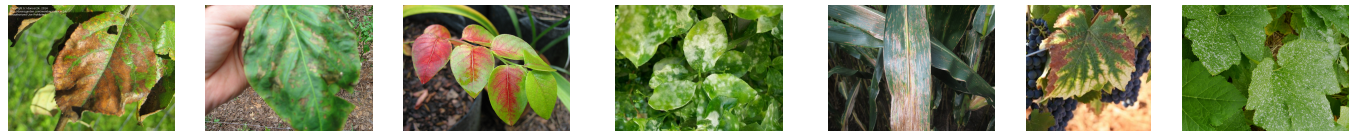
\includegraphics[width=\textwidth]{bab3/sampelplantdoc.png}
        \caption{}
        \label{fig:plantdoc_sample}
    \end{subfigure}
    
    \vspace{0.5cm}
    
    \begin{subfigure}[b]{1\textwidth}
        \centering
        \includegraphics[width=\textwidth]{bab3/plantdoc_distribution.png}
        \caption{}
        \label{fig:plantdoc_distribution_sub}
    \end{subfigure}
    \caption[Dataset PlantDoc: (a) Sampel citra dan (b) Distribusi kelas]{Dataset PlantDoc dari \textcite{singhPlantDocDatasetVisual2020}: (a) Sampel citra dan (b) Distribusi kelas}
    \label{fig:plantdoc_distribution}
\end{figure}

\paragraph{Pemodelan}
Pemodelan dilakukan dengan mengevaluasi tiga variasi skala model YOLOv11, yaitu YOLOv11n (nano), YOLOv11s (small), dan YOLOv11m (medium). Ketiga variasi model ini dipilih karena kesesuaiannya dengan target lingkungan inferensi berbasis CPU serta kebutuhan sumber daya komputasi pelatihan yang masih dapat diakomodasi oleh perangkat keras yang tersedia dalam penelitian ini. Ketiga varian ini dibandingkan untuk menentukan model yang paling optimal untuk diintegrasikan ke dalam sistem agentik. Seluruh proses pelatihan dilakukan menggunakan Ultralytics dengan konfigurasi hiperparameter bawaan, kecuali yang dirinci pada Tabel \ref{tab:yolo_hyperparameters}.

\begin{table}[H]
\centering
    \caption{Konfigurasi Hiperparameter Pelatihan YOLOv11}
    \label{tab:yolo_hyperparameters}
    \centering
    \setstretch{1.0}
    \begin{tabular}{|l|l|p{6cm}|}
\hline
    \multicolumn{1}{|c|}{\textbf{Parameter}} & \multicolumn{1}{c|}{\textbf{Nilai}} & \multicolumn{1}{c|}{\textbf{Keterangan}} \\ \hline
    Epoch & 240 & Jumlah iterasi pelatihan penuh. \\ \hline
    Input Size & 416 x 416 & Resolusi citra masukan sesuai anotasi PlantDoc. \\ \hline
    Random Seed & 42 & Menjamin keterulangan hasil eksperimen. \\ \hline
    Batch Size & 16 & Jumlah sampel per sub-iterasi. \\ \hline
    Patience & 20 & Batas iterasi tanpa peningkatan untuk \textit{early stopping}. \\ \hline
    \end{tabular}
\end{table}

Setelah proses pelatihan selesai, model diekspor ke format ONNX (\textit{Open Neural Network Exchange}) untuk meningkatkan portabilitas dan efisiensi saat dijalankan di lingkungan produksi. Proses ekspor dilakukan dengan pengaturan resolusi sesuai ukuran masukan (\textit{input size}) pada perangkat CPU guna memastikan kompatibilitas dengan keterbatasan sumber daya pada lingkungan server.

\subsubsection{Alat Deteksi Open-Vocabulary}
Alat deteksi \textit{open-vocabulary} menggunakan model OWLv2 \parencite{huggingfaceOWLv2} yang dikembangkan oleh Google \parencite{mindererScalingOpenVocabularyObject2024}. Sistem menggunakan varian model \textit{google/\allowbreak owlv2-base-\allowbreak patch16} yang telah dikonversi ke format ONNX. Model ini mengintegrasikan \textit{vision transformer} (ViT) dengan \textit{text encoder} untuk melakukan deteksi objek berdasarkan deskripsi tekstual secara \textit{zero-shot}. Gambar \ref{fig:arsitektur_owlv2} menyajikan visualisasi arsitektur dari model OWLv2.

\begin{figure}[H]
    \centering
    \includegraphics[width=1\textwidth]{bab3/arsitekturalatowlv2.png}
    \caption{Arsitektur Model OWLv2 yang Digunakan}
    \label{fig:arsitektur_owlv2}
\end{figure}

\subsection{Modul Pencarian Gambar-Teks Penyakit}
Modul pencarian gambar-teks penyakit dirancang sebagai komponen utama sistem untuk mengidentifikasi gejala penyakit tanaman melalui pendekatan pengambilan informasi multimodal. Implementasi modul ini menggunakan teknologi Qdrant yang mendukung penyimpanan dan pencarian vektor bernama jamak (\textit{multi-named vectors}) secara efisien. Melalui fitur ini, dataset yang berisi pasangan gambar dan teks dapat disematkan (\textit{embedded}) ke dalam satu koleksi Qdrant, di mana satu poin data menampung dua vektor sekaligus, yaitu vektor gambar dan vektor teks. Representasi fitur diekstraksi menggunakan model \textit{foundation} SCOLD \parencite{huggingfaceSCOLD} yang dikembangkan oleh \textcite{quocVisionLanguageFoundationModel2025} dengan arsitektur RoBERTa dari \textcite{liuRoBERTaRobustlyOptimized2019} sebagai \textit{encoder} teks dan arsitektur Swin-T dari \textcite{liuSwinTransformerHierarchical2021} sebagai \textit{encoder} gambar. Rincian lebih lanjut mengenai skema ini akan dibahas pada subbab berikutnya. Alur kerja dari modul pencarian gambar-teks divisualisasikan pada Gambar \ref{fig:image_text_search_workflow}.

\begin{figure}[H]
    \centering
    \includegraphics[width=1\textwidth]{bab3/modulgambarteks.png}
    \caption{Alur Kerja Modul Pencarian Gambar-Teks Penyakit Tanaman}
    \label{fig:image_text_search_workflow}
\end{figure}


\subsubsection{Persiapan Data Indeks}
Dataset PlantWild yang disusun oleh \textcite{weiBenchmarkingInthewildMultimodal2024} digunakan sebagai basis indeks pencarian pada modul ini. Dataset ini mencakup total 18.542 citra yang terdistribusi ke dalam 89 kelas kondisi kesehatan dan penyakit pada 13 spesies tanaman utama. Citra dalam dataset ini mencakup berbagai organ tanaman, termasuk daun, buah, dan batang. Klasifikasi tersebut terdiri dari 56 kelas penyakit dan 33 kelas kondisi sehat. Dalam penelitian ini, dilakukan pengambilan sampel secara acak sebanyak 3 citra dari setiap kelas untuk kebutuhan pengujian, sehingga diperoleh total 267 citra uji. Sebanyak 18.275 citra sisanya kemudian digunakan untuk diindeks ke dalam basis data vektor. Selain data citra, setiap kelas dalam dataset ini juga dilengkapi dengan 10 \textit{caption} yang mendeskripsikan karakteristik visual dari kelas tersebut. Gambar \ref{fig:plantwild_distribution} menyajikan distribusi kelas pada dataset PlantWild.
 
\begin{figure}[H]
    \centering
    \includegraphics[width=1\textwidth]{bab3/distribusiplantwild.png}
    \caption[Distribusi Kelas pada Dataset PlantWild]{Distribusi Kelas pada Dataset PlantWild dari \protect\textcite{weiBenchmarkingInthewildMultimodal2024}}
    \label{fig:plantwild_distribution}
\end{figure}

\subsubsection{\textit{Indexing}}
Dalam Qdrant, data dikelola dalam unit entitas yang disebut sebagai Poin (\textit{Points}). Setiap Poin terdiri dari tiga komponen utama, yaitu ID unik, vektor yang dapat berupa vektor tunggal atau jamak, dan \textit{payload} opsional untuk menyimpan metadata. Pada sistem ini, setiap entitas penyakit tanaman direpresentasikan sebagai Poin yang memiliki dua vektor padat (\textit{dense vectors}) bernama, yaitu vektor teks dan vektor citra. Citra referensi asli disimpan secara terpisah pada layanan penyimpanan objek Cloudflare R2 untuk efisiensi, sementara URL publiknya disimpan dalam \textit{payload}.

Tabel \ref{tab:qdrant_schema} menyajikan rincian skema \textit{Points} dan struktur \textit{payload} yang diimplementasikan. Skema ini dirancang untuk mendukung pencarian multimodal sekaligus penyaringan metadata yang presisi.

%TODO: perlu diperbagus tabelnya
\begin{table}[H]
    \centering
    \caption{Skema Poin (Vektor dan Payload) pada Indeks Qdrant}
    \label{tab:qdrant_schema}
    \small
    \setstretch{1.0}
    \resizebox{\textwidth}{!}{%
    \begin{tabular}{|l|l|l|p{7cm}|}
    \hline
    \multicolumn{1}{|c|}{\textbf{Komponen}} & \multicolumn{1}{c|}{\textbf{Kunci}} & \multicolumn{1}{c|}{\textbf{Tipe}} & \multicolumn{1}{c|}{\textbf{Deskripsi}} \\ \hline
    \multirow{2}{*}{\textbf{Vektor}} & \textit{text} & 512 & Representasi semantik deskripsi gejala (RoBERTa). \\ \cline{2-4} 
     & \textit{image} & 512 & Representasi fitur visual citra tanaman (Swin-T/SCOLD). \\ \hline
    \multirow{6}{*}{\textbf{Payload}} & \textit{plant\_name} & String & Nama spesies tanaman. Diindeks secara \textit{full-text} untuk filtrasi. \\ \cline{2-4} 
     & \textit{label} & String & Nama spesifik penyakit. Diindeks secara \textit{full-text}. \\ \cline{2-4} 
     & \textit{caption} & String & Deskripsi tekstual lengkap mengenai gejala. \\ \cline{2-4} 
     & \textit{image\_url} & String & Tautan publik citra di Cloudflare R2. \\ \cline{2-4} 
     & \textit{source\_id} & Integer & ID referensi internal. \\ \cline{2-4} 
     & \textit{filename} & String & Nama fail asli citra. \\ \hline
    \end{tabular}%
    }
\end{table}

Fitur penting dalam implementasi ini adalah penerapan indeks teks penuh (\textit{full-text index}) yang disediakan oleh Qdrant pada kolom \textit{payload} \textit{plant\_name} dan \textit{label}. Berbeda dengan pencocokan kata kunci eksak (\textit{keyword match}), indeks teks penuh memungkinkan agen untuk melakukan penyaringan (\textit{filtering}) yang lebih fleksibel, seperti pencocokan berdasarkan token kata (\textit{token-based matching}) dan ketidakpekaan terhadap huruf besar-kecil (\textit{case-insensitive}). Fitur ini secara signifikan meningkatkan efisiensi pencarian agen dengan membatasi ruang pencarian vektor hanya pada subset data yang relevan dengan konteks tanaman yang sedang dianalisis. Sebagai ilustrasi, ketika agen mendeteksi bahwa tanaman yang dianalisis adalah tomat, agen dapat menerapkan filter pada \textit{plant\_name} untuk hanya mencari di antara data penyakit tomat, sehingga hasil yang diperoleh lebih akurat dan relevan. Visualisasi mekanisme ini disajikan pada Gambar \ref{fig:payload_filtering}.

%TODO: ini gambar masih placeholder, sesuain konteksnya ke tanaman!
\begin{figure}[H]
    \centering
    \includegraphics[width=1\textwidth]{bab3/fulltextindexpayloadfield.png}
    \caption{Visualisasi Mekanisme Penyaringan}
    \label{fig:payload_filtering}
\end{figure}

\subsubsection{Strategi Pencarian}
Implementasi modul ini mendukung empat strategi pencarian multimodal yang memanfaatkan kemampuan representasi vektor ganda (teks dan citra) pada indeks Qdrant. Pemilihan strategi dilakukan secara dinamis oleh agen berdasarkan ketersediaan input dari pengguna (teks gejala atau citra tanaman) serta tujuan pencarian. Fleksibilitas ini dimungkinkan oleh arsitektur model SCOLD yang menyelaraskan (\textit{align}) representasi fitur teks dan citra ke dalam ruang laten yang sama, memungkinkan operasi pencarian lintas modal (\textit{cross-modal}). Keempat strategi tersebut diilustrasikan pada Gambar \ref{fig:multimodal_search_strategies} dan dijelaskan sebagai berikut:

\begin{figure}[H]
    \centering
    \begin{subfigure}[b]{0.45\textwidth}
        \centering
        \includegraphics[width=\textwidth]{bab3/strategipencarianteksteks.png}
        \caption{}
        \label{fig:strat_t2t}
    \end{subfigure}
    \hfill
    \begin{subfigure}[b]{0.45\textwidth}
        \centering
        \includegraphics[width=\textwidth]{bab3/strategipencariantekksgambar.png}
        \caption{}
        \label{fig:strat_t2i}
    \end{subfigure}
    
    \vspace{0.5cm}
    
    \begin{subfigure}[b]{0.45\textwidth}
        \centering
        \includegraphics[width=\textwidth]{bab3/strategipencariangambargambar.png}
        \caption{}
        \label{fig:strat_i2i}
    \end{subfigure}
    \hfill
    \begin{subfigure}[b]{0.45\textwidth}
        \centering
        \includegraphics[width=\textwidth]{bab3/strategipencariangambarteks.png}
        \caption{}
        \label{fig:strat_i2t}
    \end{subfigure}
    \caption{Visualisasi empat strategi pencarian multimodal: (a) \textit{Text-to-Text}, (b) \textit{Text-to-Image}, (c) \textit{Image-to-Image}, dan (d) \textit{Image-to-Text}}
    \label{fig:multimodal_search_strategies}
\end{figure}

Penjelasan rinci mengenai mekanisme kerja dari masing-masing strategi pencarian tersebut diuraikan sebagai berikut:

\begin{enumerate}[nosep]
    \item Text-to-Text (Pencarian Semantik Teks) \\
    Mode ini digunakan ketika pengguna memberikan deskripsi gejala berupa teks. Input diproses oleh \textit{tokenizer} dan \textit{text encoder} RoBERTa untuk menghasilkan vektor teks. Vektor ini kemudian dicocokkan dengan koleksi vektor teks (\textit{text}) dalam indeks Qdrant yang merepresentasikan \textit{caption} penyakit. Strategi ini efektif untuk menemukan diagnosis berdasarkan deskripsi linguistik gejala.

    \item Text-to-Image (Pencarian Lintas Modal Teks-ke-Citra) \\
    Mode ini memungkinkan pencarian citra referensi penyakit hanya dengan menggunakan deskripsi teks. Vektor teks hasil enkripsi digunakan untuk mencari tetangga terdekat pada ruang vektor citra (\textit{image}). Kemampuan ini dimungkinkan karena model SCOLD telah dilatih untuk meminimalkan jarak antara pasangan teks dan citra yang relevan dalam ruang vektor (\textit{embedding space}).

    \item Image-to-Image (Pencarian Kemiripan Visual) \\
    Mode ini adalah metode standar untuk identifikasi berbasis citra. Citra masukan dari pengguna (baik citra utuh maupun hasil potongan/crop deteksi objek) diproses oleh \textit{image encoder} (Swin-Transformer basis SCOLD) menjadi vektor citra. Vektor ini kemudian dibandingkan dengan jutaan vektor citra (\textit{image}) dalam basis data untuk menemukan penyakit dengan karakteristik visual paling serupa.

    \item Image-to-Text (Pencarian Lintas Modal Citra-ke-Teks) \\
    Mode ini membalikkan pendekatan lintas modal, di mana vektor citra masukan digunakan untuk mencari kecocokan pada ruang vektor teks (\textit{text}). Strategi ini berguna untuk mendapatkan deskripsi tekstual atau label penyakit yang paling relevan secara langsung dari fitur visual, tanpa harus bergantung pada metadata citra referensi.
\end{enumerate}


\subsection{Modul Pencarian Informasi}
Modul pencarian informasi dirancang untuk menyediakan konteks eksternal yang faktual bagi agen dalam menjawab pertanyaan pengguna atau memverifikasi hipotesis diagnosis. Agen diinstruksikan untuk memanfaatkan modul ini ketika pengguna meminta panduan manajemen penyakit atau perawatan preventif tanaman. Selain itu, modul ini berfungsi sebagai mekanisme cadangan (\textit{fallback}) faktual terakhir untuk membantu identifikasi apabila modul pencarian gambar-teks penyakit tanaman gagal memberikan hasil yang relevan, misalnya karena penyakit yang diidentifikasi tidak tersedia dalam indeks basis data vektor. Modul ini mengimplementasikan mekanisme \textit{Retrieval-Augmented Generation} (RAG) yang terdiri dari dua alat pencarian, yaitu alat pencarian pada basis data pengetahuan internal dan alat pencarian internet menggunakan Tavily API.

Basis data pengetahuan internal dibangun dari korpus dokumen terkurasi yang berfokus pada penyakit tanaman, yang disimpan dalam basis data vektor Qdrant untuk efisiensi pencarian. Dalam perancangannya, kinerja pencarian pada basis data pengetahuan dioptimalkan melalui pengujian strategi \textit{hybrid search} dan penerapan mekanisme \textit{reranking} untuk meningkatkan efesiensi pencarian. Meskipun basis data pengetahuan menawarkan informasi yang lebih terpercaya, cakupannya terbatas pada spesies tanaman yang telah diindeks. Oleh karena itu, pencarian internet melalui Tavily API diintegrasikan sebagai mekanisme cadangan (\textit{fallback}) untuk menangani kueri yang tidak dapat dijawab oleh data internal. Agen dirancang untuk memprioritaskan penggunaan pencarian basis data pengetahuan terlebih dahulu sebelum mengakses informasi dari internet. Alur kerja interaksi antara agen dan modul pencarian informasi divisualisasikan pada Gambar \ref{fig:info_search_workflow}.

\begin{figure}[H]
    \centering
    \includegraphics[width=1\textwidth]{bab3/alurkerjamodulpencarianinformasi.png}
    \caption{Alur Kerja Modul Pencarian Informasi}
    \label{fig:info_search_workflow}
\end{figure}

\subsubsection{Alat Pencarian Basis Data Pengetahuan}
Implementasi alat pencarian basis data pengetahuan diawali dengan pemilihan komponen model yang optimal melalui proses \textit{benchmarking}. Berdasarkan studi literatur, terdapat perbedaan performa antara berbagai model \textit{embedding} yang tersedia saat ini. Mengacu pada \textit{Massive Text Embedding Benchmark} (MTEB) oleh \textcite{muennighoffMTEBMassiveText2023}, model \textit{gemini-embedding-001} dari Google DeepMind tercatat sebagai model proprietari dengan peringkat teratas, mengungguli model \textit{text-embedding-3-large} dari OpenAI yang berada di peringkat kelima. Peringkat ini pada MTEB ditampilkan pada Gambar \ref{fig:mteb_benchmark}.

\begin{figure}[H]
    \centering
    \includegraphics[width=1\textwidth]{bab3/mtebbenchmark.png}
    \caption[Peringkat \textit{gemini-embedding-001} dan \textit{text-embedding-3-large} pada MTEB]{Peringkat \textit{gemini-embedding-001} dan \textit{text-embedding-3-large} pada MTEB oleh \textcite{muennighoffMTEBMassiveText2023}}
    \label{fig:mteb_benchmark}
\end{figure}

Akan tetapi, hasil yang berbeda ditunjukkan pada \textit{Semantic Alignment \& Generalization Evaluation} (SAGE) oleh \textcite{goelSAGERealisticBenchmark2025}. Pada tolok ukur ini, model \textit{text-embedding-3-large} menempati posisi terbaik dengan skor keseluruhan SAGE sebesar 0,524, sedangkan \textit{gemini-embedding-001} berada di peringkat ketiga dengan skor 0,504.

Mengingat adanya perbedaan hasil evaluasi pada berbagai tolok ukur standar tersebut, diputuskan untuk melakukan \textit{benchmarking} internal menggunakan korpus data yang akan digunakan secara riil pada sistem. Pendekatan ini diambil guna menentukan konfigurasi model yang paling sesuai dengan karakteristik unik dari data penyakit tanaman yang dikelola. Pengujian secara khusus difokuskan pada konfigurasi \textit{hybrid search}, sebuah metode yang menggabungkan keunggulan pencarian vektor padat (\textit{dense vector}) untuk menangkap konteks semantik dan vektor jarang (\textit{sparse vector}) untuk pencocokan kata kunci yang presisi. Pada komponen vektor jarang, dua pendekatan yang diuji adalah algoritma BM25 dari \textcite{robertsonProbabilisticRelevanceFramework2009} yang berbasis frekuensi kata dan tersedia di Qdrant, serta model SPLADE dari \textcite{formalSPLADESparseLexical2021} yang berbasis pembelajaran mesin dan dijalankan melalui FastEmbed. Kombinasi pengujian ini dirancang untuk mencakup empat variasi konfigurasi \textit{hybrid search}, yaitu: (1) \textit{text-embedding-3-large} yang dipadukan dengan BM25, (2) \textit{text-embedding-3-large} dengan SPLADE, (3) \textit{gemini-embedding-001} dengan BM25, dan (4) \textit{gemini-embedding-001} dengan SPLADE.

Konfigurasi \textit{hybrid search} yang menunjukkan kinerja terbaik selanjutnya akan dibawa ke tahap pengujian lanjutan untuk mengevaluasi efektivitas penambahan komponen \textit{reranker}. Pengujian pada tahap ini bertujuan untuk membandingkan kinerja antara dua arsitektur model \textit{reranking} yang berbeda, yakni model berbasis \textit{cross-encoder} dan model dengan pendekatan \textit{late interaction}. Sebagai representasi dari model \textit{cross-encoder}, dipilih model \textit{rerank-2.5} dari Voyage AI yang memproses kueri dan dokumen secara bersamaan untuk akurasi tinggi. Sementara itu, untuk pendekatan \textit{late interaction}, digunakan model \textit{jina-colbert-v2} dari Jina AI \parencite{jhaJinaColBERTv2GeneralPurposeMultilingual2024} yang diimplementasikan melalui pustaka FastEmbed. Perbandingan ini dilakukan untuk memastikan diperolehnya konfigurasi \textit{Retrieval-Augmented Generation} (RAG) yang paling optimal dan andal sebelum diimplementasikan sepenuhnya ke dalam sistem agentik. Keseluruhan alur pengujian komponen pencarian ini, mulai dari pemilihan strategi pencarian hingga pemeringkatan ulang, divisualisasikan secara rinci pada Gambar \ref{fig:alur_pengujian_retrieval}.

\begin{figure}[H]
    \centering
    \includegraphics[width=0.8\textwidth]{bab3/alurkerjabenchmarkrag.png}
    \caption{Diagram Alur Pengujian Komponen Alat Pencarian Basis Data Pengetahuan}
    \label{fig:alur_pengujian_retrieval}
\end{figure}

\paragraph{Persiapan Data Korpus}
Persiapan data korpus untuk basis pengetahuan dilakukan melalui serangkaian tahapan mulai dari pengumpulan data mentah melalui \textit{web scraping}, penyusunan korpus, hingga pembangkitan dataset evaluasi sintetis. Alur kerja lengkap persiapan data ini divisualisasikan pada Gambar \ref{fig:data_preparation_workflow}.

\begin{figure}[H]
    \centering
    \begin{tikzpicture}[
        node distance=0.5cm,
        font=\scriptsize,
        start/.style={circle, draw, fill=blue!10, minimum size=1.2cm, align=center},
        process/.style={rectangle, draw, rounded corners, fill=blue!5, align=center, minimum width=3cm, minimum height=0.8cm},
        data/.style={cylinder, shape border rotate=90, draw, aspect=0.25, fill=yellow!10, align=center, minimum width=2cm, minimum height=0.8cm},
        model/.style={ellipse, draw, dashed, fill=green!5, align=center, minimum width=2cm},
        arrow/.style={-stealth, thick}
    ]

    % Nodes
    \node (start) [start] {Mulai};
    \node (sources) [process, fill=white, below=of start] {Sumber Data\\(PlantVillage \& Gardenology)};
    \node (crawl) [process, below=of sources] {Crawling URL\\(Playwright/Crawl4AI)};
    \node (scrape) [process, below=of crawl] {Scraping \& Ekstraksi\\(ScrapeGraphAI)};
    \node (llm_scrape) [model, right=0.5cm of scrape] {LLM:\\Gemini 2.5 Flash};

    \node (json) [data, below=of scrape] {Data JSON\\(222 Entri)};

    \node (chunk) [process, below=of json] {Semantic Chunking\\(LlamaIndex)};
    \node (embed) [model, right=0.5cm of chunk] {Embedding:\\Gemini Emb-001};

    \node (corpus) [data, below=of chunk] {Korpus Dokumen\\(2.469 Dokumen)};

    \node (gen_qa) [process, below=of corpus] {Pembangkitan QA\\(AutoRAG Strategy)};
    \node (llm_qa) [model, right=0.5cm of gen_qa] {LLM:\\Gemini 2.5 Flash};

    \node (dataset) [data, below=of gen_qa, fill=green!20] {Dataset QA\\(600 Sampel)};

    \node (end) [start, below=of dataset] {Selesai};

    % Arrows
    \draw [arrow] (start) -- (sources);
    \draw [arrow] (sources) -- (crawl);
    \draw [arrow] (crawl) -- (scrape);
    \draw [arrow] (scrape) -- (json);
    \draw [arrow] (json) -- (chunk);
    \draw [arrow] (chunk) -- (corpus);
    \draw [arrow] (corpus) -- (gen_qa);
    \draw [arrow] (gen_qa) -- (dataset);

    \draw [arrow] (dataset) -- (end);

    \draw [arrow, dashed] (llm_scrape) -- (scrape);
    \draw [arrow, dashed] (embed) -- (chunk);
    \draw [arrow, dashed] (llm_qa) -- (gen_qa);

    \end{tikzpicture}
    \caption{Alur Kerja Persiapan Data Dari Crawling hingga Pembangkitan Dataset QA}
    \label{fig:data_preparation_workflow}
\end{figure}

%TODO: ini mungkin perlu sitasi ajh webnya
Data mentah dikumpulkan dari dua sumber utama, yaitu PlantVillage (plantvillage.psu.edu) dan Gardenology (gardenology.org). PlantVillage dipilih karena reputasinya sebagai sumber informasi penyakit tanaman yang kredibel yang dikelola oleh Penn State University, sedangkan Gardenology dipilih untuk melengkapi informasi mengenai aspek budidaya dan propagasi tanaman yang kurang mendalam pada PlantVillage.

\begin{figure}[H]
    \centering
    \begin{subfigure}[b]{0.48\textwidth}
        \centering
        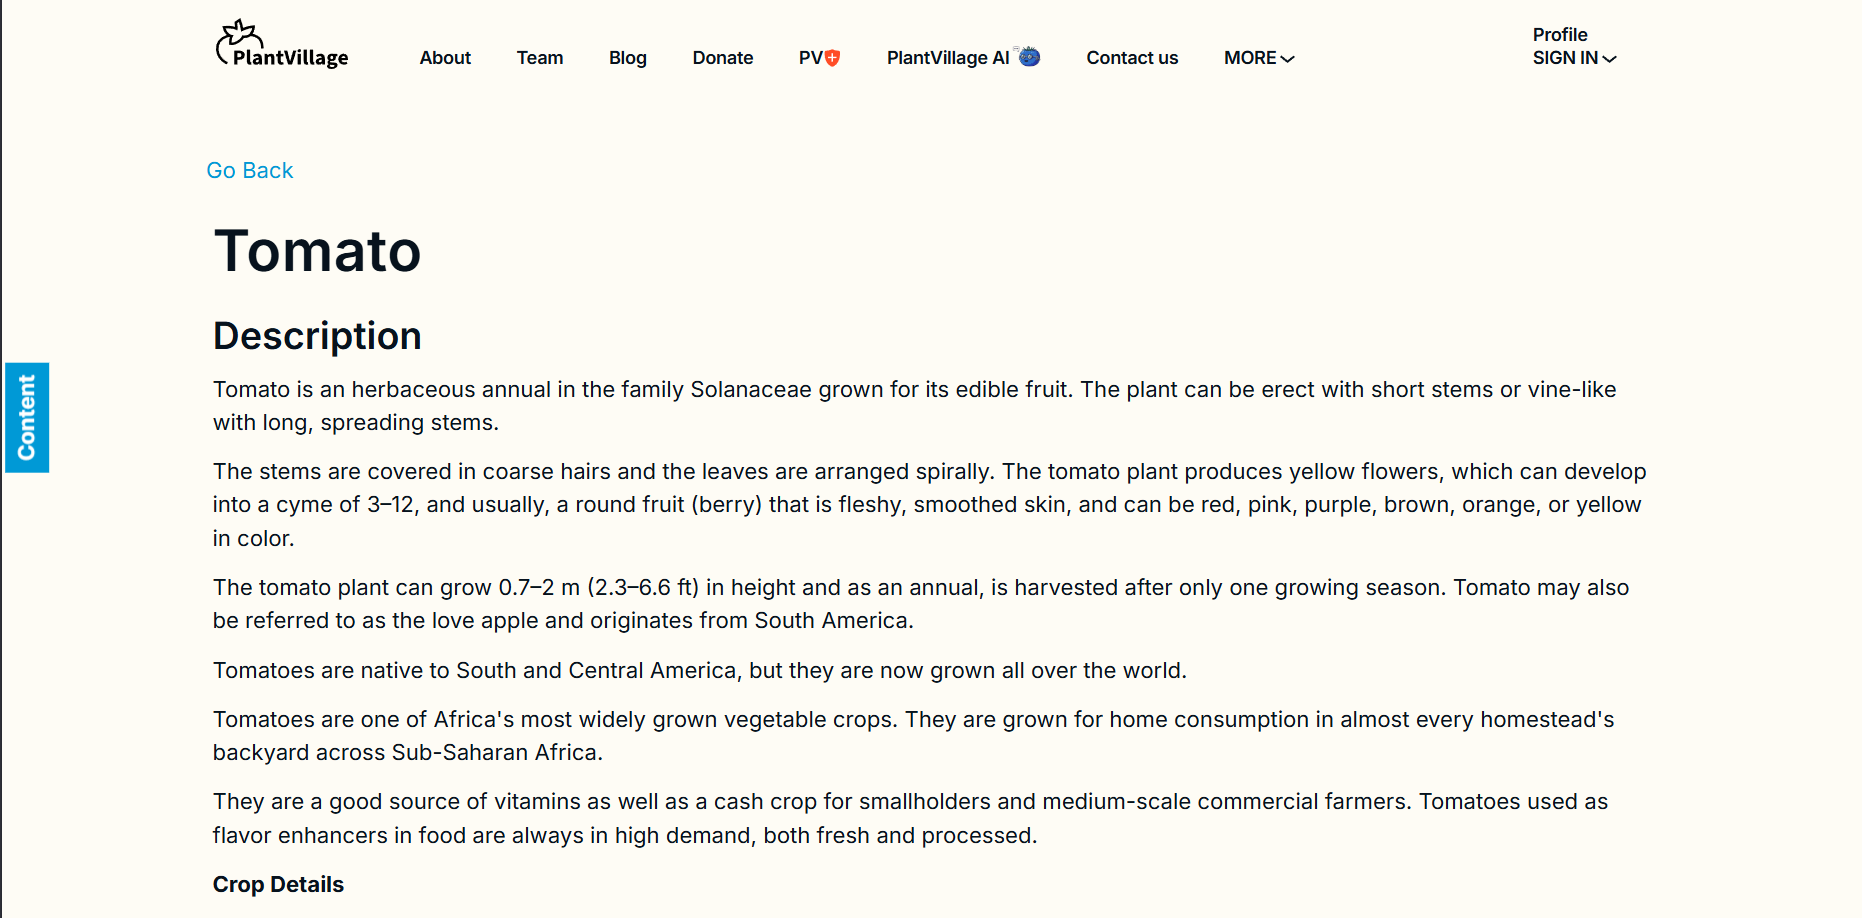
\includegraphics[width=\textwidth]{bab3/plantvillageweb.png}
        \caption{}
        \label{fig:plantvillage_web}
    \end{subfigure}
    \hfill
    \begin{subfigure}[b]{0.48\textwidth}
        \centering
        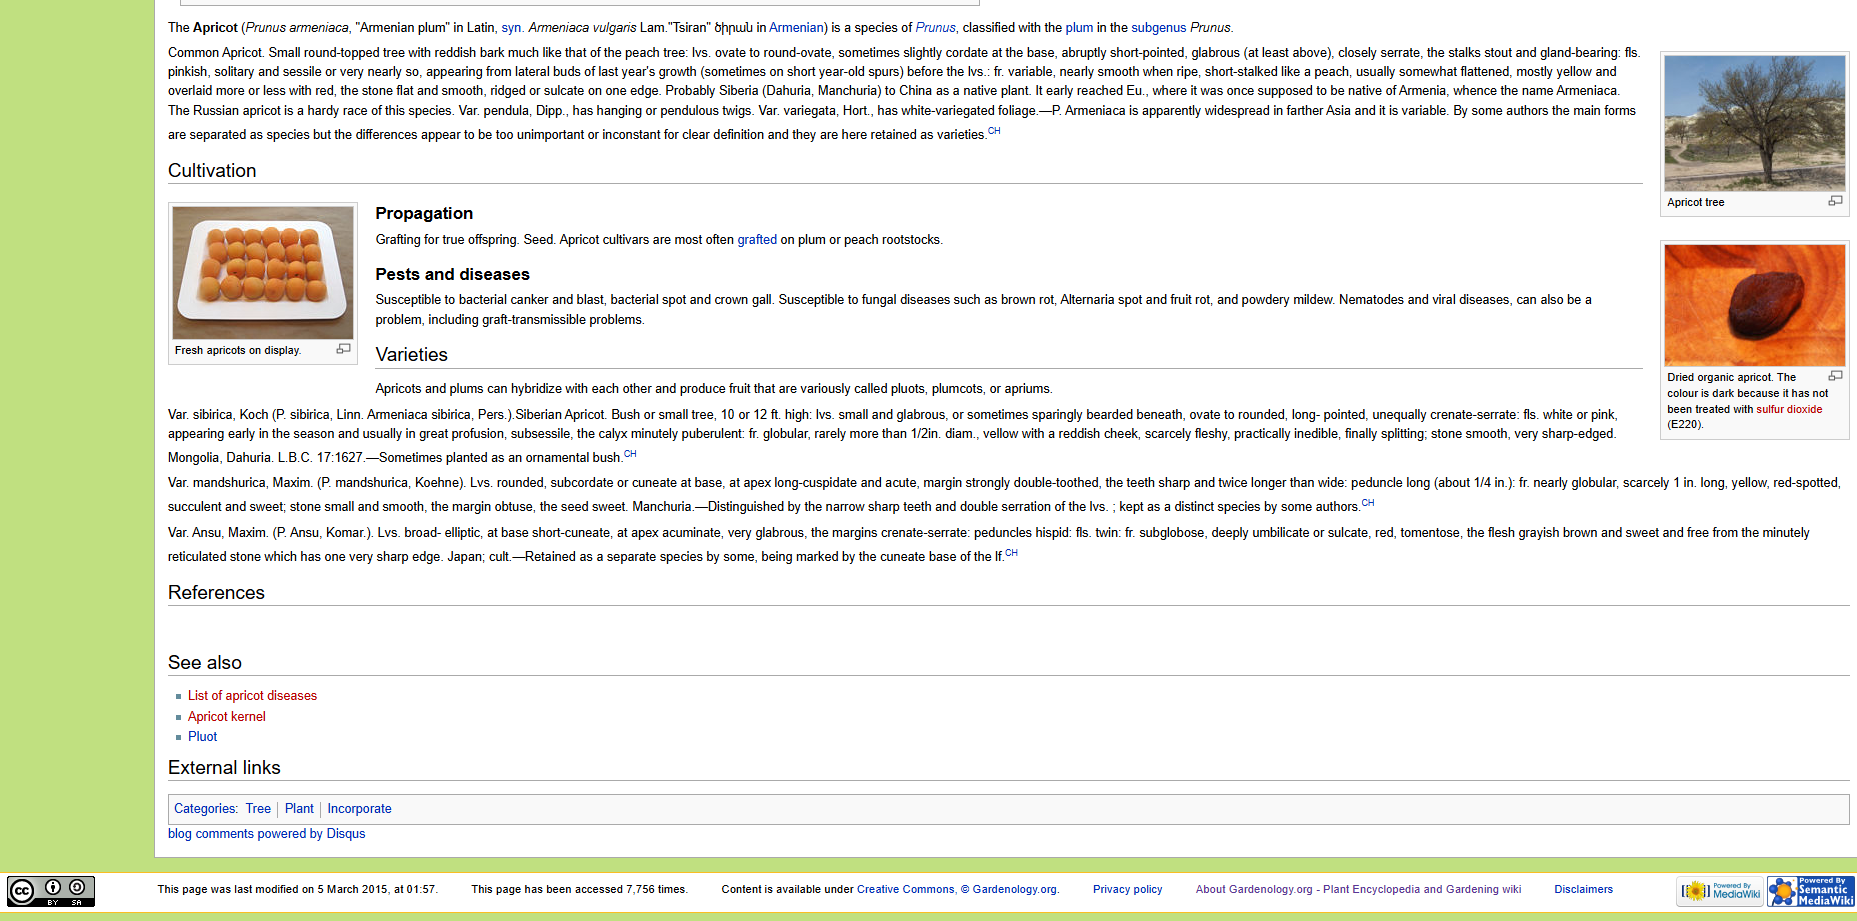
\includegraphics[width=\textwidth]{bab3/gardenologyweb.png}
        \caption{}
        \label{fig:gardenology_web}
    \end{subfigure}
    \caption{Tampilan antarmuka situs sumber data: (a) PlantVillage dan (b) Gardenology}
    \label{fig:sumber_data_web}
\end{figure}

Proses pengumpulan data dilakukan menggunakan teknik \textit{web scraping} hibrida yang menggabungkan automasi peramban (\textit{browser automation}) dan ekstraksi berbasis LLM. Untuk penemuan tautan (\textit{crawling}), digunakan pustaka Playwright dari Python. Selanjutnya, ekstraksi konten dilakukan menggunakan pustaka ScrapeGraphAI. Pustaka ini memanfaatkan LLM untuk mengurai struktur HTML yang tidak beraturan menjadi format JSON yang terstruktur sesuai skema yang didefinisikan. Model Gemini 2.5 Flash dengan temperatur 0 dipilih sebagai otak ekstraksi karena memiliki jendela konteks (\textit{context window}) yang besar dan latensi rendah. Tabel \ref{tab:scraping_schema} menyajikan skema data yang digunakan untuk ekstraksi. Dari proses ini, berhasil dikumpulkan 222 entri data yang mencakup sekitar 200 spesies tanaman unik.

\begin{table}[H]
    \centering
    \caption{Skema Ekstraksi Data dari PlantVillage dan Gardenology}
    \label{tab:scraping_schema}
    \small
    \begin{tabular}{|l|l|p{7cm}|}
    \hline
    \textbf{Atribut} & \textbf{Tipe Data} & \textbf{Deskripsi} \\ \hline
    \textit{plant} & String & Nama umum tanaman. \\ \hline
    \textit{description} & String & Deskripsi umum karakteristik tanaman. \\ \hline
    \textit{propagation} & String & Informasi budidaya tanaman. \\ \hline
    \textit{pests\_and\_diseases} & List/String & Daftar penyakit beserta gejala, penyebab, dan manajemennya. \\ \hline
    \end{tabular}
\end{table}

Data JSON hasil \textit{scraping} kemudian diproses menjadi korpus dokumen menggunakan kerangka kerja LlamaIndex. Informasi dipisahkan menjadi dua kategori dokumen utama, yaitu (1) dokumen budidaya/propagasi dan (2) dokumen penyakit. Untuk menangani dokumen teks yang panjang, diterapkan teknik pemotongan semantik (\textit{semantic chunking}) menggunakan \textit{SemanticSplitterNodeParser} dari LlamaIndex dengan model \textit{embedding} \textit{gemini-embedding-001}. Pemotongan semantik bekerja dengan menghitung jarak kosinus (\textit{cosine distance}) antar representasi vektor dari kalimat-kalimat yang berurutan. Dalam implementasinya, ditetapkan parameter \textit{breakpoint percentile threshold} sebesar 95. Nilai ini menginstruksikan algoritma untuk menentukan ambang batas pemotongan berdasarkan persentil ke-95 dari distribusi jarak semantik dalam dokumen. Dengan kata lain, pemisahan dokumen (\textit{splitting}) hanya dilakukan pada titik-titik yang memiliki tingkat perbedaan semantik tertinggi (top 5\%), yang mengindikasikan adanya pergantian topik atau konteks yang signifikan. Pendekatan ini memastikan bahwa setiap potongan dokumen (\textit{chunk}) memiliki koherensi tematik yang utuh dan tidak terpotong di tengah penjelasan yang relevan. Proses ini menghasilkan total 2.469 potongan dokumen (\textit{chunks}) yang siap diindeks. Contoh sampel dokumen hasil pemotongan semantik dapat dilihat pada Gambar \ref{fig:sampel_korpus}.

\begin{figure}[H]
    \centering
    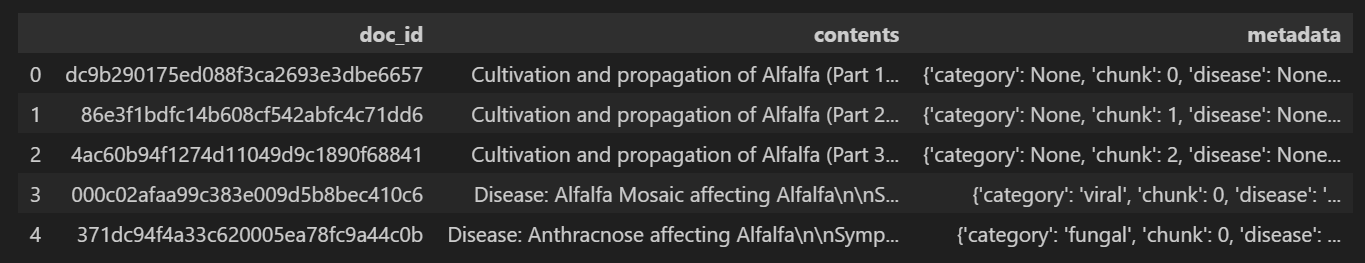
\includegraphics[width=1\textwidth]{bab3/sampelkorpus.png}
    \caption{Sampel korpus dokumen hasil pemotongan semantik}
    \label{fig:sampel_korpus}
\end{figure}

Untuk mengevaluasi performa pada \textit{benchmarking}, dibuat dataset \textit{Question-Answering} (QA) sintetis sebanyak 600 sampel dari korpus yang telah disusun. Pembangkitan dilakukan menggunakan Gemini 2.5 Flash dengan temperatur 0 dan dalam bahasa Inggris. Pembangkitan dataset ini menggunakan dan mengadopsi metodologi yang disediakan AutoRAG dari \textcite{kimAutoRAGAutomatedFramework2024}. Dataset mencakup tiga jenis pertanyaan dengan tingkat kompleksitas berbeda, sebagaimana dirangkum dalam Tabel \ref{tab:qa_types}.

\begin{table}[H]
    \centering
    \caption{Jenis Pertanyaan pada Dataset Evaluasi QA Sintetis}
    \label{tab:qa_types}
    \small
    \resizebox{\textwidth}{!}{
    \begin{tabular}{|l|p{4cm}|p{6cm}|c|}
    \hline
    \textbf{Tipe Pertanyaan} & \textbf{Definisi} & \textbf{Contoh} & \textbf{Proporsi} \\ \hline
    \textit{Factoid Single Hop} & Pertanyaan yang mencari fakta singkat dan spesifik yang dapat diverifikasi. & "Apa patogen penyebab penyakit hawar daun pada tomat?" & 35\% \\ \hline
    \textit{Concept Completion} & Pertanyaan yang menanyakan esensi atau definisi dari suatu konsep. & "Jelaskan karakteristik dari gejala klorosis." & 35\% \\ \hline
    \textit{Two-Hop Incremental} & Pertanyaan multi-lompatan yang membutuhkan inferensi dari dua segmen informasi berbeda \parencite{hwangExplainableMultihopQuestion2024}. & "Bagaimana cara menangani penyakit yang disebabkan oleh jamur Fusarium pada tanaman pisang?" & 30\% \\ \hline
    \end{tabular}
    }
\end{table}

\paragraph{Indexing}
Proses pengindeksan dilakukan dengan memanfaatkan fitur vektor bernama jamak (\textit{multi-named vectors}) pada Qdrant. Fitur ini memungkinkan penyimpanan beberapa representasi vektor sekaligus dalam satu entitas Poin (\textit{Point}) tunggal. Pendekatan ini diterapkan untuk memfasilitasi evaluasi strategi pencarian yang komprehensif dengan menyatukan seluruh representasi vektor dari berbagai model dalam satu koleksi terpadu. Setiap dokumen dalam korpus diubah menjadi Poin yang memiliki empat komponen vektor, yaitu dua vektor padat (\textit{dense vectors}) dan dua vektor jarang (\textit{sparse vectors}). Vektor padat dihasilkan oleh model \textit{gemini-embedding-001} dan \textit{text-embedding-3-large}, masing-masing dengan dimensi 3.072. Sementara itu, vektor jarang dihasilkan menggunakan model SPLADE++ dan algoritma BM25 yang terintegrasi secara internal di Qdrant.

Selain representasi vektor, setiap Poin juga menyimpan \textit{payload} yang berisi konten teks dokumen dan metadata terkait. Untuk mendukung efisiensi pengambilan informasi oleh agen, diterapkan indeks teks penuh (\textit{full-text index}) pada atribut metadata nama tanaman (\textit{metadata.plant}) dan nama penyakit (\textit{metadata.disease}). Penggunaan indeks teks penuh memungkinkan agen untuk melakukan penyaringan (\textit{filtering}) berbasis token kata terhadap ruang pencarian, sehingga hasil yang diperoleh lebih relevan dengan konteks tanaman atau penyakit yang sedang dianalisis. Skema lengkap representasi data pada indeks basis pengetahuan disajikan pada Tabel \ref{tab:knowledge_base_schema}.

\begin{table}[H]
    \centering
    \caption{Skema Poin dengan Vektor Jamak dan Metadata pada Basis Data Pengetahuan}
    \label{tab:knowledge_base_schema}
    \small
    \setstretch{1.0}
    \resizebox{\textwidth}{!}{%
    \begin{tabular}{|l|l|l|p{7cm}|}
    \hline
    \textbf{Komponen} & \textbf{Kunci} & \textbf{Tipe} & \textbf{Deskripsi} \\ \hline
    \multirow{2}{*}{\textbf{Vektor Padat}} & \textit{gemini} & 3.072 & Representasi semantik dari Gemini Embedding. \\ \cline{2-4} 
     & \textit{openai} & 3.072 & Representasi semantik dari OpenAI Embedding. \\ \hline
    \multirow{2}{*}{\textbf{Vektor Jarang}} & \textit{splade} & Variabel & Representasi leksikal dari SPLADE++. \\ \cline{2-4} 
     & \textit{bm25} & Variabel & Skor relevansi berbasis frekuensi kata (BM25). \\ \hline
    \multirow{5}{*}{\textbf{Payload}} & \textit{page\_content} & String & Konten teks lengkap dari dokumen. \\ \cline{2-4} 
     & \textit{metadata.plant} & String & Nama tanaman. Diindeks secara \textit{full-text}. \\ \cline{2-4} 
     & \textit{metadata.disease} & String & Nama penyakit. Diindeks secara \textit{full-text}. \\ \cline{2-4} 
     & \textit{metadata.type} & String & Jenis dokumen (budidaya/penyakit). \\ \cline{2-4} 
     & \textit{metadata.source} & String & Sumber dokumen (PlantVillage/Gardenology). \\ \hline
    \end{tabular}%
    }
\end{table}
%TODO(Human): Perlu di-update visualisasi ini yang ngeliatin semua mode pencariannya (image-text, image-image, text-text, text-image)

\paragraph{Strategi Pencarian}
Implementasi strategi pencarian pada modul ini dirancang untuk memaksimalkan relevansi dokumen melalui pendekatan bertingkat. Proses pencarian diawali dengan memberikan akses agen LLM untuk menerapkan filter metadata (seperti nama tanaman, penyakit, atau jenis dokumen) untuk membatasi ruang pencarian hanya pada entitas yang relevan. Selanjutnya, sistem melakukan pencarian hibrida yang menggabungkan hasil dari representasi vektor padat (\textit{dense embedding}) dan vektor jarang (\textit{sparse embedding}).

Pada tahap pencarian hibrida, sistem dikonfigurasi agar agen LLM dapat melakukan pengambilan awal (\textit{prefetching}) terhadap sejumlah kandidat dokumen yang lebih besar, yakni sebesar $2k$, dari masing-masing indeks vektor. Hasil dari kedua jalur pencarian ini kemudian disatukan menggunakan algoritma \textit{Reciprocal Rank Fusion} (RRF). Algoritma ini memberikan bobot skor berdasarkan peringkat kemunculan dokumen di setiap daftar hasil, dengan tujuan memprioritaskan dokumen yang secara konsisten dinilai relevan oleh kedua metode pencarian. Mekanisme penilaian skor \textit{Reciprocal Rank Fusion} (RRF) tersebut dirumuskan pada Persamaan \ref{eq:rrf}.

\begin{equation}
    score(d \in D) = \sum_{r_d \in R(d)} \frac{1}{k + r_d}
    \label{eq:rrf}
\end{equation}
    \daftarpersamaan{Reciprocal Rank Fusion (RRF)}

\begin{figure}[H]
    \centering
    \includegraphics[width=1\textwidth]{bab3/alatpencarianbasispengetahuan.png}
    \caption{Visualisasi Alur Kerja Strategi Pencarian Hibrida pada Basis Data Pengetahuan}
    \label{fig:knowledge_base_search_workflow}
\end{figure}

\subsubsection{Alat Pencarian Internet}
Alat pencarian internet diimplementasikan menggunakan Tavily Search API. Tavily merupakan mesin pencari yang dioptimasi khusus untuk sistem agentik (\textit{agentic systems}) dengan tujuan memberikan hasil pencarian yang efisien, cepat, dan konsisten \parencite{tavilyaiTavilyaiTavilypython2026}. Penggunaan API ini memungkinkan sistem untuk mengabstraksi serangkaian proses kompleks dalam pengambilan informasi daring, yang mencakup pencarian, \textit{web scraping}, penyaringan konten, pemeringkatan ulang (\textit{re-ranking}), hingga ekstraksi informasi yang paling relevan secara otomatis.

Konfigurasi parameter yang digunakan dalam inisialisasi alat pencarian ini dirinci pada Tabel \ref{tab:tavily_parameters}. Parameter \textit{max\_results} diatur untuk mengembalikan lima dokumen teratas guna memberikan variasi sumber informasi yang cukup bagi agen. Topik pencarian diatur ke "general" untuk memastikan cakupan sumber yang luas. Selain itu, fitur pencarian gambar diaktifkan untuk memperkaya konteks visual yang dapat diberikan kepada pengguna.

\begin{table}[H]
    \centering
    \caption{Konfigurasi Parameter Tavily Search API}
    \label{tab:tavily_parameters}
    \small
    \resizebox{\textwidth}{!}{%
    \begin{tabular}{|l|l|p{7cm}|}
    \hline
    \textbf{Parameter} & \textbf{Nilai} & \textbf{Deskripsi} \\ \hline
    \textit{max\_results} & 5 & Jumlah maksimal hasil dokumen yang dikembalikan. \\ \hline
    \textit{topic} & "general" & Kategori topik pencarian untuk cakupan sumber umum. \\ \hline
    \textit{search\_depth} & "advanced" & Kedalaman pencarian untuk hasil yang lebih komprehensif. \\ \hline
    \textit{include\_images} & \textit{True} & Mengembalikan tautan gambar yang relevan. \\ \hline
    \textit{include\_image\_descriptions} & \textit{True} & Menyertakan deskripsi tekstual untuk gambar yang ditemukan. \\ \hline
    \end{tabular}
    }
\end{table}

\subsection{Antarmuka Sistem Agentik}
Antarmuka sistem dikembangkan sebagai media interaksi utama antara pengguna dan sistem agentik yang telah dibangun. Pengembangan ini bertujuan untuk memfasilitasi akses terhadap fitur identifikasi penyakit tanaman secara intuitif melalui platform berbasis web.

\subsubsection{Arsitektur Antarmuka}
Sistem antarmuka dibangun dengan memisahkan komponen sisi klien (\textit{frontend}) dan sisi server (\textit{backend}) guna memastikan skalabilitas dan kemudahan pemeliharaan. Arsitektur sistem secara keseluruhan terdiri dari dua komponen utama:

\begin{enumerate}[nosep]
    \item Aplikasi Web (\textit{Frontend}): Komponen ini merupakan aplikasi web berbasis Next.js yang mengadopsi \textit{Agent Chat UI} dari \textcite{langchainLangchainaiAgentchatui2026}. Aplikasi ini bertanggung jawab untuk merender antarmuka percakapan, mengelola unggahan berkas, serta menampilkan visualisasi pemanggilan alat (\textit{tool calls}) secara waktu nyata (\textit{real-time}). Dalam implementasinya, aplikasi web ini di-\textit{hosting} pada platform Vercel.
    \item LangGraph Server (\textit{Backend}): Komponen ini berfungsi sebagai infrastruktur yang menyerupai arsitektur tanpa peladen (\textit{serverless-like}) yang menjalankan logika agen LangGraph secara berstatus (\textit{stateful}). Server menyediakan titik akhir (API) yang dioptimalkan untuk komunikasi asinkron, manajemen utas (\textit{thread}), dan persistensi status percakapan. Komponen sistem agentik ini dikemas dalam kontainer dan diterapakan pada layanan \textit{cloud container} Google Cloud Run.
\end{enumerate}

Seluruh komponen yang beroperasi secara lokal dan berinteraksi dengan sistem agentik, seperti koleksi basis data vektor Qdrant serta model-model inferensi yang ada pada setiap modul, diintegrasikan dalam satu lingkungan kontainer menggunakan Docker. Integrasi ini bertujuan untuk menyederhanakan proses penerapan (\textit{deployment}) serta memastikan konsistensi operasional sistem pada berbagai lingkungan penampungan (\textit{hosting}). Visualisasi arsitektur sistem secara garis besar (\textit{high-level}) disajikan pada Gambar \ref{fig:high_level_architecture}.

\begin{figure}[H]
    \centering
    \includegraphics[width=0.7\textwidth]{bab3/arsitekturantarmukasistem.png}
    \caption{Arsitektur antarmuka sistem agentik}
    \label{fig:high_level_architecture}
\end{figure}

\subsubsection{Use Case Diagram}
Fungsionalitas antarmuka sistem agentik dipetakan melalui \textit{Use Case Diagram} untuk memberikan gambaran mengenai interaksi aktor dengan sistem. Aktor utama dalam sistem ini adalah Pengguna yang berinteraksi langsung dengan aplikasi web. Gambar \ref{fig:use_case_diagram} menyajikan pemetaan fungsionalitas utama yang tersedia pada antarmuka.

\begin{figure}[H]
    \centering
    \includegraphics[width=0.8\textwidth]{bab3/usecasediagram.png}
    \caption{Use Case Diagram Antarmuka Sistem Agentik}
    \label{fig:use_case_diagram}
\end{figure}

Penjelasan dari fungsionalitas tersebut adalah sebagai berikut:
\begin{enumerate}[nosep]
    \item Interaksi Multimodal: Pengguna dapat mengirimkan instruksi berupa teks (seperti pertanyaan tentang gejala) serta mengunggah citra (daun, buah, atau bagian tanaman lainnya) sebagai input utama proses identifikasi.
    \item Visualisasi Hasil: Sistem menampilkan respons AI secara \textit{streaming} beserta beserta keluaran setiap alat ke pengguna.
    \item Transparansi Agen: Pengguna dapat memantau langkah-langkah internal agen (penggunaan alat deteksi, pencarian web, dll) secara transparan untuk memverifikasi proses pengambilan keputusan.
    \item Manajemen Konteks: Pengguna dapat menyimpan, mengganti nama, atau menghapus sesi percakapan untuk mengelola riwayat identifikasi yang telah dilakukan sebelumnya.
\end{enumerate}

\subsubsection{Sequence Diagram}
Alur komunikasi dan koordinasi antar komponen dalam sistem agentik dipetakan melalui \textit{Sequence Diagram}. Diagram ini memberikan gambaran mengenai urutan pertukaran pesan dan data antar aktor serta komponen sistem dalam satu skenario tugas identifikasi penyakit tanaman. Gambar \ref{fig:sequence_diagram} memvisualisasikan urutan interaksi sistem dari input pengguna hingga pemberian diagnosis akhir secara sistematis untuk memastikan integritas data dan responsivitas.

\begin{figure}[H]
    \centering
    \includegraphics[width=1\textwidth]{bab3/sequencediagram.png}
    \caption{Diagram Urutan Interaksi Identifikasi Penyakit Tanaman}
    \label{fig:sequence_diagram}
\end{figure}

Secara lebih rinci, arsitektur sistem terdiri dari tiga lapisan utama yang bekerja sama untuk memfasilitasi interaksi pengguna dengan agen cerdas, yaitu:
\begin{enumerate}[nosep]
    \item \textit{Frontend}: Bertindak sebagai antarmuka pengguna yang menangani tampilan visual, penyimpanan kunci API secara lokal, manajemen \textit{state} sementara dengan React, serta pengiriman permintaan ke server.
    \item LangGraph Server API: Berperan sebagai orkestrator yang mengelola siklus hidup \textit{thread} (kontainer percakapan) dan \textit{run} (eksekusi), menyediakan titik akhir API, serta menangani antrian eksekusi untuk \textit{background worker}.
    \item Sistem Agentik: Menjalankan logika bisnis utama dan mengeksekusi graf, termasuk pemanggilan alat eksternal seperti basis data dan model AI untuk menghasilkan respons.
\end{enumerate}

Interaksi antara ketiga komponen tersebut dibagi menjadi tiga skenario utama, yaitu pengiriman pesan baru, akses \textit{thread} lama, dan pengiriman pesan lanjutan.

Skenario pertama adalah pengiriman pesan baru, baik pada \textit{thread} baru maupun \textit{thread} yang sudah ada. Sebagaimana diperlihatkan pada Gambar \ref{fig:seq_submit}, proses dimulai ketika pengguna mengirimkan pesan yang kemudian diteruskan oleh \textit{frontend} ke API untuk membuat \textit{run} baru. \textit{Run} tersebut dimasukkan ke dalam antrian untuk diproses oleh \textit{background worker}. Sistem agentik kemudian mengeksekusi graf secara lengkap, mulai dari pengambilan citra, inferensi model, hingga pencarian vektor, dan mengalirkan hasilnya (\textit{streaming}) kembali ke antarmuka pengguna secara waktu nyata.

\begin{figure}[H]
    \centering
    \includegraphics[width=1\textwidth]{bab3/sequencediagramsubmit.png}
    \caption{Diagram Urutan Pengiriman Pesan Baru}
    \label{fig:seq_submit}
\end{figure}

Skenario kedua menjelaskan mekanisme akses ke \textit{thread} lama melalui riwayat percakapan. Pada skenario ini, yang divisualisasikan pada Gambar \ref{fig:seq_access_thread}, tidak terjadi panggilan API ke LangGraph Server untuk eksekusi graf. \textit{Frontend} hanya melakukan resolusi konfigurasi (seperti ID asisten dan URL API) dan menyinkronkan \textit{state} dengan parameter URL. Riwayat percakapan ditampilkan menggunakan data yang telah tersedia tanpa memicu proses komputasi ulang di sisi agen.

\begin{figure}[H]
    \centering
    \includegraphics[width=1\textwidth]{bab3/sequencediagramaksesthreadlama.png}
    \caption{Diagram Urutan Akses \textit{Thread} Sebelumnya}
    \label{fig:seq_access_thread}
\end{figure}

Skenario ketiga menunjukkan alur ketika pengguna melanjutkan percakapan pada \textit{thread} yang sama (\textit{resubmit}), sebagaimana ditunjukkan pada Gambar \ref{fig:seq_resubmit}. Dalam kondisi ini, server membuat \textit{run} baru yang dikonfigurasi untuk menggunakan status (\textit{state}) dari \textit{thread} sebelumnya sebagai konteks. Hal ini memungkinkan agen untuk memproses pesan baru dengan tetap mempertahankan memori dari interaksi sebelumnya, memastikan kesinambungan percakapan yang relevan.

\begin{figure}[H]
    \centering
    \includegraphics[width=1\textwidth]{bab3/submitulangdithreadlama.png}
    \caption{Diagram Urutan Melanjutkan Percakapan pada \textit{Thread} Lama}
    \label{fig:seq_resubmit}
\end{figure}

\subsubsection{Prototipe Antarmuka}
Prototipe antarmuka merupakan representasi visual awal dari sistem yang dikembangkan untuk memberikan gambaran interaksi pengguna. Antarmuka pada sistem ini diadopsi dari proyek sumber terbuka \textit{Agent Chat UI} yang dikembangkan oleh \textcite{langchainLangchainaiAgentchatui2026}. Desain antarmuka dirancang dengan pendekatan minimalis untuk memfokuskan perhatian pengguna pada interaksi percakapan dan hasil identifikasi.

Gambar \ref{fig:prototipe_antarmuka} memperlihatkan tampilan utama dari prototipe antarmuka. Pada bagian kiri terdapat panel sisi (\textit{sidebar}) yang menampilkan riwayat percakapan (\textit{Thread History}) pengguna. Bagian tengah didominasi oleh area interaksi utama yang memuat logo sistem, kolom input pesan, dan tombol aksi. Kolom input dilengkapi dengan fitur untuk mengunggah berkas citra atau dokumen PDF, serta tombol geser (\textit{toggle}) untuk menyembunyikan atau menampilkan detail pemanggilan alat (\textit{tool calls}) oleh agen.

\begin{figure}[H]
    \centering
    \includegraphics[width=1\textwidth]{bab3/prototipeantarmuka.png}
    \caption{Tampilan prototipe antarmuka sistem agentik}
    \label{fig:prototipe_antarmuka}
\end{figure}


\section{Pengujian}
Tahap pengujian dilakukan untuk memvalidasi fungsionalitas dari setiap komponen sistem yang telah dikembangkan sebelum dilakukan evaluasi kinerja secara menyeluruh. Pengujian ini mencakup verifikasi operasional pada modul deteksi objek, modul pencarian gambar-teks, modul pencarian informasi, serta antarmuka pengguna.

\subsection{Modul Deteksi Objek Tanaman}
Pengujian fungsionalitas modul deteksi objek dilakukan untuk memverifikasi kemampuan integrasi model YOLOv11 dan OWLv2 dalam lingkungan sistem. Pengujian dilakukan dengan memberikan citra masukan yang mengandung objek daun serta citra dengan objek tanaman lain seperti buah atau batang. Indikator keberhasilan pengujian adalah sistem mampu menghasilkan kotak pembatas (\textit{bounding box}) yang tepat pada objek yang relevan dan mengembalikan koordinat serta label kelas yang sesuai untuk diproses oleh tahap selanjutnya.

\subsection{Modul Pencarian Gambar-Teks Penyakit}
Pengujian modul pencarian gambar-teks difokuskan pada validasi fungsional dari empat strategi pencarian yang telah diimplementasikan, yaitu \textit{text-to-text}, \textit{text-to-image}, \textit{image-to-image}, dan \textit{image-to-text}. Setiap strategi diuji dengan memberikan input yang sesuai (teks atau gambar) dan memeriksa relevansi hasil pencarian yang dikembalikan oleh basis data vektor Qdrant. Pengujian ini bertujuan untuk memastikan bahwa mekanisme \textit{embedding} dan \textit{retrieval} berfungsi dengan baik dalam berbagai modalitas input.

\subsection{Modul Pencarian Informasi}
Pengujian pada modul pencarian informasi dilakukan untuk memastikan konektivitas dan responsivitas dari dua alat pencarian utama, yaitu pencarian basis data pengetahuan internal dan pencarian internet melalui Tavily API. Pengujian dilakukan dengan mengirimkan kueri terkait manajemen penyakit dan memverifikasi apakah sistem dapat mengambil dokumen yang relevan dari korpus internal atau tautan eksternal yang valid.

\subsection{Antarmuka Sistem Agentik}
Pengujian antarmuka dilakukan menggunakan metode \textit{Black Box Testing} untuk memastikan bahwa seluruh fungsionalitas yang telah dirancang pada \textit{Use Case Diagram} dapat beroperasi sesuai dengan ekspektasi pengguna. \textit{Black Box Testing} merupakan metode pengujian perangkat lunak yang berfokus pada spesifikasi fungsional sistem \parencite{bhasinBlackBoxTesting2014}. Pengujian fungsionalitas antarmuka dirangkum dalam Tabel \ref{tab:black_box_testing_expected}.

\begin{table}[H]
    \centering
    \caption{Pengujian \textit{Black Box} Antarmuka Sistem Agentik}
    \label{tab:black_box_testing_expected}
    \small
    \setstretch{1.0}
    \resizebox{\textwidth}{!}{
    \begin{tabular}{|l|l|p{4.5cm}|p{5cm}|}
    \hline
    ID & Fitur & Skenario Pengujian & Hasil yang Diharapkan \\ \hline
    \textbf{UC1} & Mengirim Prompt & Pengguna mengetik instruksi pada kolom teks (\textit{textarea}) dan menekan tombol kirim (ikon \textit{ArrowUp}). & Sistem mengirim pesan ke server dan menampilkan respons agen secara bertahap (\textit{streaming}). \\ \hline
    \textbf{UC2} & Mengunggah Citra Tanaman & Pengguna mengklik ikon \textit{Paperclip} untuk memilih gambar atau menyeret berkas langsung ke area percakapan. & Gambar muncul sebagai \textit{preview} di atas kolom input dan berhasil dikirim bersama pesan teks. \\ \hline
    \textbf{UC3} & Melihat Hasil \& Saran & Pengguna menunggu proses inferensi selesai setelah mengirimkan kueri identifikasi. & Jawaban berupa diagnosis penyakit dan panduan penanganan muncul secara lengkap di area chat. \\ \hline
    \textbf{UC4} & Mengelola Riwayat Percakapan & Pengguna memilih sesi pada \textit{sidebar}, mengubah nama sesi, atau mengirim pesan baru pada sesi lama. & Riwayat dimuat, nama sesi berubah, dan agen memproses pesan baru dengan konteks sesi tersebut. \\ \hline
    \textbf{UC5} & Melihat Transparansi Agen & Pengguna menekan tombol kontrol alat (ikon \textit{Wrench}) untuk mengaktifkan visibilitas proses. & Detail pemanggilan alat (\textit{tool calls}) dan hasil observasi internal agen ditampilkan di antara pesan chat. \\ \hline
    \end{tabular}
    }
\end{table}

\subsection{Sistem Agentik}
Tahapan pengujian dan evaluasi dilakukan untuk memvalidasi kinerja sistem agentik secara komprehensif. Seluruh rangkaian pengujian ini diorkestrasi menggunakan platform LangSmith. Platform ini difungsikan sebagai pusat manajemen pengujian yang mencakup pengelolaan \textit{prompt} dan teknik \textit{prompt engineering} untuk sistem agen LLM, manajemen dataset pengujian, serta analisis hasil eksperimen secara terpusat.

Rangkaian pengujian dibagi menjadi dua kategori utama yang dibahas pada subbab-subbab berikut, yaitu pengujian satu tahap untuk mengukur kapabilitas penyelesaian tugas tunggal dan pengujian multi-tahap untuk mengevaluasi konsistensi interaksi dalam percakapan berkelanjutan.

\subsubsection{Pengujian Satu Tahap}
Pengujian satu tahap difokuskan pada evaluasi kemampuan agen dalam menyelesaikan tugas identifikasi dan tanya jawab dalam satu giliran interaksi tunggal. Pengujian ini terdiri dari eksperimen VQA (\textit{Visual Question Answering}). Pengujian ini merupakan pengujian utama yang dilakukan untuk mengevaluasi kinerja sistem secara menyeluruh. Skenario ini dirancang untuk merepresentasikan interaksi dunia nyata di mana pengguna mengunggah gambar tanaman beserta pertanyaan teks terkait kondisinya. Dalam eksperimen ini, seluruh kapabilitas sistem akan diuji secara terintegrasi, meliputi kemampuan pemahaman konteks multimodal, akurasi identifikasi penyakit visual, ketepatan pengambilan informasi dari basis pengetahuan, kesesuaian penggunaan alat, serta kualitas dan relevansi jawaban yang diberikan kepada pengguna.

\paragraph{Persiapan Data}
Dataset yang digunakan dalam pengujian satu tahap dikelompokkan menjadi dua jenis berdasarkan distribusi datanya, yaitu dataset \textit{In-Distribution} (ID) dan dataset \textit{Out-of-Distribution} (OOD).

\subparagraph{\textit{Dataset In-Distribution} (ID)}
Dataset ID merepresentasikan data yang berada dalam cakupan distribusi pengetahuan internal sistem. Data ini diambil dari subset dataset PlantWild yang telah digunakan dalam penyusunan indeks pencarian gambar-teks. Sebagaimana dijelaskan pada bagian sebelumnya, dataset ini mencakup 18.542 citra dari 89 kelas kondisi kesehatan pada 13 spesies tanaman. Untuk keperluan pengujian, dilakukan pengambilan sampel acak sebanyak 3 citra dari setiap kelas, sehingga diperoleh total 267 citra uji. Penggunaan sampel ini bertujuan untuk memvalidasi kemampuan sistem dalam mengenali dan mengambil informasi yang sudah pernah dipelajari atau diindeks sebelumnya.

\subparagraph{\textit{Dataset Out-of-Distribution} (OOD)}
Dataset OOD disusun untuk menguji ketangguhan (\textit{robustness}) dan kemampuan generalisasi sistem dalam menangani kueri yang melibatkan spesies tanaman atau jenis penyakit yang tidak terdapat dalam basis pengetahuan internal. Dataset ini dikompilasi dari berbagai dataset publik yang mencakup 8 komoditas tanaman berbeda dengan total 40 kelas penyakit dan kondisi kesehatan unik. Rincian sumber data untuk setiap komoditas disajikan pada Tabel \ref{tab:ood_datasets}.

\begin{table}[H]
    \centering
    \caption{\textit{Rincian Dataset Out-of-Distribution} (OOD)}
    \label{tab:ood_datasets}
    \small
    \setstretch{1.0}
    \resizebox{\textwidth}{!}{
    \begin{tabular}{|l|l|c|l|}
    \hline
    \textbf{No.} & \textbf{Komoditas} & \textbf{Kelas} & \textbf{Sumber Referensi} \\ \hline
    1. & Cabai Merah & 5 & \textcite{mpChilliDataset2024} \\ \hline
    2. & Kacang Hitam & 5 & \textcite{talasilaBlackGramPlant2022} \\ \hline
    3. & Bayam Malabar & 5 & \textcite{sayeemIDDMSLDImageDataset2025} \\ \hline
    4. & Okra & 6 & \textcite{kumarakuruOkraDiseaseNetDataset2024} \\ \hline
    5. & Lobak & 5 & \textcite{rashidImageDatasetRadish2024} \\ \hline
    6. & Jambu Biji & 7 & \textcite{shihabImageDatasetDetection2024} \\ \hline
    7. & Gandum & 3 & \textcite{getachewWheatLeafDataset2021} \\ \hline
    8. & Bawang Bombay & 4 & \textcite{mpOnionDataset2024} \\ \hline
    \multicolumn{2}{|c|}{\textbf{Total}} & \textbf{40} & - \\ \hline
    \end{tabular}
    }
\end{table}

Serupa dengan prosedur pada dataset ID, dilakukan pengambilan sampel acak sebanyak 3 citra untuk setiap kelas pada dataset OOD, menghasilkan total 120 citra uji. Citra-citra tersebut kemudian diunggah ke layanan penyimpanan objek Cloudflare R2 untuk mendapatkan URL publik. Selanjutnya, metadata untuk setiap sampel disusun dalam format JSON. Metadata ini mencakup label penyakit, status kesehatan, \textit{caption} gejala visual, serta informasi manajemen penyakit yang dikurasi dari sumber ilmiah otoritatif. Informasi manajemen penyakit ini disertakan sebagai \textit{ground truth} untuk mengevaluasi kualitas saran yang diberikan oleh agen. Contoh entri dataset evaluasi OOD disajikan pada Gambar \ref{fig:ood_json_example}.

\begin{figure}[H]
    \centering
    \includegraphics[width=1\textwidth]{bab3/contohentri.png}
    \caption{Contoh Entri Dataset Evaluasi OOD dalam Format JSON}
    \label{fig:ood_json_example}
\end{figure}

Selanjutnya, dataset evaluasi diperkaya melalui proses pembangkitan data sintetis menggunakan LLM Gemini 2.5 Flash. Proses ini bertujuan untuk mensimulasikan variasi interaksi pengguna yang mungkin terjadi di dunia nyata. Model LLM diberikan akses terhadap citra asli beserta metadata JSON yang telah disusun sebelumnya untuk membangkitkan pasangan pertanyaan-jawaban (\textit{QA pairs}) yang kontekstual. Baik pada dataset ID maupun OOD, untuk setiap citra uji dibangkitkan tiga variasi skenario pertanyaan sebagai berikut:

\begin{enumerate}[nosep]
    \item Skenario 1: Pengguna diasumsikan sebagai orang awam yang mendeskripsikan gejala visual secara samar namun menyebutkan spesies tanaman.
    \item Skenario 2: Pengguna dianggap sudah mengetahui spesies tanaman dan langsung menanyakan konfirmasi mengenai penyakit tertentu atau meminta saran penanganan spesifik.
    \item Skenario 3: Pengguna tidak memiliki pengetahuan mengenai spesies maupun gejala spesifik. Pertanyaan yang diajukan bersifat umum seperti "Kenapa tanaman saya?" atau "Apakah ini penyakit?".
\end{enumerate}

Logika yang sama juga diterapkan untuk kelas tanaman sehat. Khusus untuk Skenario 1 pada tanaman sehat, deskripsi difokuskan pada kondisi visual tanaman yang menunjukkan ciri-ciri pertumbuhan normal. Untuk memastikan kualitas data yang dihasilkan, diterapkan teknik \textit{few-shot prompting} dalam instruksi yang diberikan kepada LLM. Contoh \textit{prompt} yang digunakan untuk Skenario 1 disajikan pada Gambar \ref{fig:prompt_scenario_1}.

\begin{figure}[H]
    \centering
    \includegraphics[width=1\textwidth]{bab3/contohpromptpersiapandata.png}
    \caption{Contoh Prompt Few-Shot untuk Skenario 1}
    \label{fig:prompt_scenario_1}
\end{figure}

Proses pembangkitan dataset ini dilakukan melalui alur kerja terstruktur untuk menjamin validitas dan konsistensi format keluaran. Setiap citra diproses melalui tahapan validasi kualitas, analisis komposisi visual, penentuan logika penggunaan alat, hingga generasi konten akhir. Alur instruksi yang diberikan kepada LLM dalam proses ini divisualisasikan pada Gambar \ref{fig:dataset_generation_pipeline}.

\begin{figure}[H]
    \centering
    \begin{tikzpicture}[
        scale=0.8, transform shape,
        node distance=1.0cm,
        font=\scriptsize,
        start/.style={circle, draw, fill=blue!10, minimum size=1cm, align=center},
        process/.style={rectangle, draw, rounded corners, fill=white, minimum width=3cm, minimum height=0.8cm, align=center},
        decision/.style={diamond, draw, fill=yellow!10, aspect=2, inner sep=0pt, minimum width=2cm, align=center},
        arrow/.style={-stealth, thick},
        io/.style={trapezium, trapezium left angle=70, trapezium right angle=110, draw, fill=green!10, minimum width=2.5cm, align=center}
    ]

    \node (start) [start] {Mulai};
    \node (input) [io, below=of start] {Citra Masukan};
    \node (model) [process, below=of input] {Gemini 2.5 Flash};
    \node (qc) [process, below=of model] {Validasi Kualitas\\(Quality Control)};
    \node (check) [decision, below=of qc] {Terkait\\Tanaman?};
    \node (discard) [process, right=2cm of check, fill=red!10] {Buang/Filter};

    \node (analysis) [process, below=of check] {Analisis Komposisi\\(Daun/Non-Daun)};
    \node (logic) [process, below=of analysis] {Penentuan Alat\\(Tool Logic)};
    \node (gen) [process, below=of logic] {Generasi Konten\\(User Text, Goal, Answer)};
    \node (output) [io, below=of gen] {JSON Output};

    \draw [arrow] (input) -- (model);
    \draw [arrow] (start) -- (input);
    \draw [arrow] (model) -- (qc);
    \draw [arrow] (qc) -- (check);
    \draw [arrow] (check) -- node[above] {Tidak} (discard);
    \draw [arrow] (check) -- node[right] {Ya} (analysis);
    \draw [arrow] (analysis) -- (logic);
    \draw [arrow] (logic) -- (gen);
    \draw [arrow] (gen) -- (output);

    \node (end) [start, below=of output] {Selesai};

    \draw [arrow] (discard) |- (end);
    \draw [arrow] (output) -- (end);

    \end{tikzpicture}
    \caption{Alur instruksi pembangkitan dataset sintetis dengan LLM}
    \label{fig:dataset_generation_pipeline}
\end{figure}

{\small Hasil akhir dari proses generasi ini disimpan dalam format JSON yang terstruktur. Struktur ini mencakup input simulasi pengguna, luaran referensi yang diharapkan (\textit{ground truth}), serta metadata pendukung. Contoh entri dataset hasil generasi untuk ketiga skenario disajikan pada Gambar \ref{fig:synthetic_dataset_examples}. \par}

\begin{figure}[H]
    \centering
    \begin{subfigure}[b]{\textwidth}
        \centering
        \includegraphics[width=\textwidth]{bab3/contohskenario1.png}
        \caption{}
    \end{subfigure}
    \hfill
    \begin{subfigure}[b]{\textwidth}
        \centering
        \includegraphics[width=\textwidth]{bab3/contohskenario2.png}
        \caption{}
    \end{subfigure}
    \hfill
    \begin{subfigure}[b]{\textwidth}
        \centering
        \includegraphics[width=\textwidth]{bab3/contohskenario3.png}
        \caption{}
    \end{subfigure}
    \caption{Contoh Entri Dataset Evaluasi Sintetis: (a) Skenario 1, (b) Skenario 2, dan (c) Skenario 3}
    \label{fig:synthetic_dataset_examples}
\end{figure}

\subsubsection{Pengujian Multi-Tahap}
Pengujian multi-tahap dalam penelitian ini difokuskan pada eksperimen Batasan Domain (\textit{Domain Boundary}). Eksperimen ini bertujuan untuk menguji ketahanan sistem dalam menjaga konsistensi peran dan relevansi topik selama interaksi percakapan yang berlangsung dalam beberapa giliran (\textit{multi-turn}). Pengujian ini diorkestrasi menggunakan fitur simulasi interaksi dari platform LangSmith, di mana agen dihadapkan dengan "pengguna simulasi" (\textit{simulated user}) yang dijalankan oleh LLM lain dengan instruksi persona tertentu. Pendekatan ini memungkinkan evaluasi yang dinamis terhadap respons agen saat menghadapi berbagai skenario percakapan yang berkembang.

\paragraph{Persiapan Data}
Persiapan data dilakukan dengan menyusun dataset yang berisi 10 contoh skenario interaksi. Setiap skenario dilengkapi dengan pesan awal pengguna dan instruksi sistem untuk pengguna simulasi guna membentuk persona yang spesifik. Variasi persona yang digunakan dalam pengujian ini dikelompokkan sebagai berikut:

\begin{enumerate}[nosep]
    \item \textit{On-topic Personas}: Persona pengguna yang mengajukan pertanyaan relevan mengenai kesehatan tanaman, baik disertai bukti visual maupun teks saja. Contoh persona ini meliputi Petani Tomat, Penghobi Mawar, dan Petani Cabai.
    \item \textit{Off-topic Personas}: Persona pengguna yang secara eksplisit meminta bantuan di luar domain keahlian agen. Contohnya mencakup pemilik mobil yang meminta saran mekanis, investor yang menanyakan harga saham, dan pertanyaan medis terkait kesehatan manusia.
    \item \textit{Edge Cases}: Skenario batas yang menguji kemampuan diskriminasi visual agen, seperti pengguna yang mengirimkan foto tanaman artifisial atau objek hewan (misalnya kucing) untuk melihat apakah agen dapat membedakan objek non-tanaman.
    \item \textit{Context Switchers}: Persona yang dirancang untuk menguji fleksibilitas agen dalam menangani perpindahan topik. Kategori ini mencakup perpindahan dari topik tanaman ke topik lain (\textit{On-to-Off}) untuk menguji ketegasan agen, serta perpindahan dari topik umum ke topik tanaman (\textit{Off-to-On}) untuk menguji responsivitas agen terhadap pertanyaan valid setelah penolakan awal.
\end{enumerate}

\section{Evaluasi}
Tahap evaluasi bertujuan untuk mengukur kinerja kuantitatif dari komponen-komponen utama sistem serta kualitas luaran akhir sistem agentik menggunakan metrik-metrik standar dan kustom.

\subsection{Modul Deteksi Objek Tanaman}
Evaluasi model deteksi dilakukan untuk mengukur ketepatan lokalisasi dan klasifikasi objek. Metrik yang digunakan meliputi \textit{Precision}, \textit{Recall}, \textit{F1-score}, serta \textit{mean Average Precision} (mAP) pada ambang batas IoU 50\% (mAP50) dan rentang 50--95\% (mAP50-95). Definisi metrik tersebut diuraikan sebagai berikut:

\begin{enumerate}[nosep]
    \item IoU (\textit{Intersection over Union}): Mengukur tingkat tumpang tindih antara kotak prediksi ($BB_{pred}$) dan \textit{ground truth} ($BB_{gt}$). Secara praktis, metrik ini menunjukkan seberapa presisi model dalam melokalisasi posisi objek daun yang sebenarnya sebagaimana ditunjukkan pada Persamaan \ref{eq:iou}.
    \begin{equation}
        IoU = \frac{Area(BB_{pred} \cap BB_{gt})}{Area(BB_{pred} \cup BB_{gt})}
        \label{eq:iou}
    \end{equation}
    \daftarpersamaan{Intersection over Union (IoU)}

    \item Precision: Rasio prediksi positif yang benar terhadap total prediksi positif. Metrik ini mengindikasikan tingkat kepercayaan terhadap prediksi model, yakni seberapa sering model benar ketika menyatakan mendeteksi daun dan meminimalkan deteksi palsu, sebagaimana dirumuskan pada Persamaan \ref{eq:precision}.
    \begin{equation}
        Precision = \frac{TP}{TP + FP}
        \label{eq:precision}
    \end{equation}
    \daftarpersamaan{Precision}

    \item Recall: Rasio prediksi positif yang benar terhadap total sampel positif aktual. Metrik ini mengukur sensitivitas model, yakni kemampuannya untuk menemukan seluruh objek daun yang ada dalam citra dan meminimalkan objek yang terlewat, seperti yang dinyatakan dalam Persamaan \ref{eq:recall}.
    \begin{equation}
        Recall = \frac{TP}{TP + FN}
        \label{eq:recall}
    \end{equation}
    \daftarpersamaan{Recall}

    \item F1-score: Rata-rata harmonis antara \textit{precision} dan \textit{recall}. Metrik ini memberikan gambaran keseimbangan performa model, memastikan model tidak hanya berhati-hati dalam mendeteksi tetapi juga mampu menemukan objek sebanyak mungkin, yang dihitung menggunakan Persamaan \ref{eq:f1}.
    \begin{equation}
        F1 = 2 \cdot \frac{Precision \cdot Recall}{Precision + Recall}
        \label{eq:f1}
    \end{equation}
    \daftarpersamaan{F1-score}

    \item mAP (\textit{mean Average Precision}): Rata-rata \textit{Average Precision} (AP) di seluruh kelas. Metrik ini merupakan standar evaluasi menyeluruh yang merepresentasikan keandalan model pada berbagai tingkat ambang batas deteksi, sebagaimana didefinisikan pada Persamaan \ref{eq:map}.
    \begin{equation}
        mAP = \frac{1}{N} \sum_{i=1}^{N} AP_i
        \label{eq:map}
    \end{equation}
    \daftarpersamaan{Mean Average Precision (mAP)}
\end{enumerate}

Selain metrik akurasi, evaluasi performa waktu atau latensi inferensi dilakukan untuk mengukur efisiensi model saat dijalankan pada perangkat dengan sumber daya terbatas. Pengukuran latensi dilakukan melalui prosedur \textit{benchmarking} yang dirancang untuk mensimulasikan kondisi penggunaan nyata. Proses ini diawali dengan mengekspor model ke format ONNX (\textit{Open Neural Network Exchange}) dan dijalankan menggunakan \textit{engine} ONNX Runtime dengan penyedia eksekusi CPU (\textit{CPU Execution Provider}).

Prosedur pengujian terdiri dari dua tahap, yaitu fase pemanasan (\textit{warm-up}) dan fase pengujian utama. Fase pemanasan dilakukan sebanyak 30 iterasi untuk menstabilkan performa sistem dan memastikan model telah dimuat sepenuhnya ke dalam memori. Selanjutnya, fase pengujian utama dilakukan sebanyak 300 iterasi menggunakan citra yang dipilih secara acak dari dataset. Pada setiap iterasi, waktu eksekusi dicatat untuk tiga komponen proses: (1) prapemrosesan, yang meliputi \textit{resizing} citra ke resolusi $416 \times 416$ piksel, normalisasi, dan penyusunan \textit{batch}; (2) inferensi model; dan (3) pascapemrosesan, yang meliputi penskalaan koordinat dan penerapan \textit{Non-Maximum Suppression} (NMS). Latensi total dihitung sebagai akumulasi dari ketiga tahapan tersebut. Alur kerja prosedur \textit{benchmarking} ini diilustrasikan pada Gambar \ref{fig:benchmark_flowchart}.

\begin{figure}[H]
    \centering
    \begin{tikzpicture}[
        node distance=1.0cm,
        font=\small,
        start/.style={circle, draw, fill=blue!10, minimum size=1cm, align=center},
        process/.style={rectangle, draw, rounded corners, fill=white, minimum width=3.5cm, minimum height=0.8cm, align=center},
        decision/.style={diamond, draw, fill=yellow!10, aspect=2, inner sep=0pt, minimum width=2.5cm, align=center},
        arrow/.style={-stealth, thick}
    ]

    \node (start) [start] {Mulai};
    \node (init) [process, below=of start] {Inisialisasi Model ONNX\\\& Sampel Citra};
    \node (warmup) [process, below=of init] {Fase Pemanasan\\(30 Iterasi)};
    
    \node (iter_start) [decision, below=of warmup] {Iterasi Uji\\$<$ 300?};
    
    \node (pre) [process, below=0.8cm of iter_start] {Prapemrosesan\\(Resize, Normalize)};
    \node (infer) [process, below=0.5cm of pre] {Inferensi Model\\(ONNX Runtime CPU)};
    \node (post) [process, below=0.5cm of infer] {Pascapemrosesan\\(NMS, Scaling)};
    \node (record) [process, below=0.5cm of post] {Catat Latensi Total};
    
    \node (calc) [process, right=1.5cm of iter_start] {Hitung Statistik\\(p50, p95)};
    \node (end) [start, below=of calc] {Selesai};

    \draw [arrow] (start) -- (init);
    \draw [arrow] (init) -- (warmup);
    \draw [arrow] (warmup) -- (iter_start);
    
    \draw [arrow] (iter_start) -- node[right] {Ya} (pre);
    \draw [arrow] (pre) -- (infer);
    \draw [arrow] (infer) -- (post);
    \draw [arrow] (post) -- (record);
    
    \draw [arrow] (record.west) -- ++(-0.5,0) |- (iter_start.west);
    
    \draw [arrow] (iter_start) -- node[above] {Tidak} (calc);
    \draw [arrow] (calc) -- (end);

    \end{tikzpicture}
    \caption{Diagram Alur Prosedur \textit{Benchmarking} Latensi Model}
    \label{fig:benchmark_flowchart}
\end{figure}

Data latensi yang dikumpulkan dari fase pengujian kemudian dianalisis secara statistik menggunakan metrik persentil ke-50 (p50) dan persentil ke-95 (p95). Misalkan $T = \{t_1, t_2, \dots, t_n\}$ adalah himpunan waktu latensi total yang telah diurutkan secara menaik, definisi dan relevansi praktis dari kedua metrik tersebut adalah:

\begin{enumerate}[nosep]
    \item p50 (Median): Merepresentasikan nilai tengah dari distribusi latensi. Metrik ini menggambarkan kecepatan respons tipikal yang akan dialami oleh mayoritas pengguna dalam penggunaan normal. Secara matematis, p50 dapat dihitung menggunakan Persamaan \ref{eq:p50}:
    \begin{equation}
        p50 = \begin{cases} t_{\frac{n+1}{2}} & \text{jika } n \text{ ganjil} \\ \frac{1}{2} (t_{\frac{n}{2}} + t_{\frac{n}{2}+1}) & \text{jika } n \text{ genap} \end{cases}
        \label{eq:p50}
    \end{equation}
    \daftarpersamaan{Latensi p50 (Median)}

    \item p95 (Persentil ke-95): Merepresentasikan ambang batas waktu di mana 95\% dari total sampel inferensi lebih cepat dari nilai tersebut. Metrik ini digunakan untuk mengukur performa dalam skenario terburuk (\textit{tail latency}), memastikan sistem tetap responsif bahkan saat memproses citra yang kompleks atau dalam kondisi beban tinggi. Nilai p95 dihitung sesuai Persamaan \ref{eq:p95}:
    \begin{equation}
        p95 = t_{\lceil 0.95 \cdot n \rceil}
        \label{eq:p95}
    \end{equation}
    \daftarpersamaan{Latensi p95 (Persentil ke-95)}
\end{enumerate}

Setelah tahap evaluasi, dilakukan \textit{benchmarking} dengan menganalisis hubungan antara mAP dan latensi melalui grafik \textit{Pareto frontier}. Grafik \textit{Pareto frontier} digunakan untuk mengidentifikasi sekumpulan model yang memberikan kombinasi performa terbaik tanpa ada model lain yang lebih unggul di kedua aspek secara bersamaan \parencite{shakyaSmallObjectDetectionEdge2026}. Visualisasi contoh grafik \textit{Pareto frontier} disajikan pada Gambar \ref{fig:pareto_curve}. Analisis ini bertujuan untuk mengidentifikasi varian model yang menawarkan latensi paling minimal dengan tetap mempertahankan performa deteksi yang optimal.

\begin{figure}[H]
    \centering
    \includegraphics[width=0.9\textwidth]{bab3/contohparetofrontier.png}
    \caption[Contoh Grafik \textit{Pareto Frontier} mAP vs Latensi]{Contoh Grafik \textit{Pareto Frontier} mAP vs Latensi \parencite{shakyaSmallObjectDetectionEdge2026}}
    \label{fig:pareto_curve}
\end{figure}

\subsection{Modul Pencarian Informasi}
Evaluasi kinerja modul pencarian informasi dilakukan secara \textit{offline} menggunakan pustaka \textit{ranx} oleh \textcite{bassaniRanxBlazingFastPython2022}. Evaluasi ini bertujuan untuk mengukur efektivitas berbagai strategi pencarian dan konfigurasi model yang telah diimplementasikan dalam menemukan dokumen relevan dari korpus basis data pengetahuan.

Persiapan evaluasi dimulai dengan penyusunan \textit{Query Relevance Judgments} (Qrels). Qrels merupakan standar kebenaran (\textit{ground truth}) yang memetakan setiap kueri dengan dokumen-dokumen yang dianggap relevan. Dalam penelitian ini, struktur Qrels direpresentasikan dalam format \textit{dictionary} Python sesuai dengan spesifikasi \textit{ranx}, di mana setiap ID kueri memiliki daftar ID dokumen relevan beserta skor relevansinya.

Skor relevansi yang digunakan bersifat biner, di mana nilai 1 diberikan untuk dokumen yang relevan dan secara implisit nilai 0 untuk dokumen lainnya. Hal ini didasarkan pada fakta bahwa dataset QA sintetis dibangun dengan memasangkan kueri secara spesifik pada potongan dokumen sumber tertentu, sehingga relevansi dapat ditentukan secara deterministik.

Proses evaluasi dilakukan dengan membandingkan hasil pencarian sistem (\textit{Run}) terhadap Qrels menggunakan serangkaian metrik standar dalam pencarian informasi. Mengingat penggunaan model \textit{embedding} dan LLM yang mutakhir (\textit{State-of-the-Art}), evaluasi difokuskan pada peringkat atas (Top-K) yang ketat, yaitu dengan nilai $k=5$. Pemilihan $k$ yang kecil ini bertujuan untuk memastikan sistem benar-benar menyajikan informasi yang paling relevan pada urutan teratas, sehingga meminimalkan beban kognitif pengguna dalam memilah informasi.

Berikut adalah metrik-metrik yang digunakan dalam evaluasi:

\begin{enumerate}[noitemsep]
    \item \textit{Mean Reciprocal Rank} (MRR) \\
    MRR mengukur rata-rata kebalikan dari peringkat dokumen relevan pertama yang ditemukan. Metrik ini sangat krusial untuk jenis pertanyaan faktual di mana pengguna hanya membutuhkan satu jawaban yang benar secepat mungkin. Nilai MRR dihitung dengan Persamaan \ref{eq:mrr}:
    \begin{equation}
        MRR = \frac{1}{|Q|} \sum_{i=1}^{|Q|} \frac{1}{rank_i}
        \label{eq:mrr}
    \end{equation}
    \daftarpersamaan{Mean Reciprocal Rank (MRR)}
    di mana $|Q|$ adalah jumlah kueri dan $rank_i$ adalah posisi peringkat dokumen relevan pertama untuk kueri ke-$i$.

    \item \textit{Normalized Discounted Cumulative Gain} (NDCG@k) \\
    NDCG@k mengevaluasi kualitas pemeringkatan dengan mempertimbangkan posisi dokumen relevan dalam daftar hasil. Dokumen relevan yang muncul di posisi lebih tinggi akan memberikan kontribusi skor yang lebih besar. Metrik ini dihitung dengan membagi \textit{Discounted Cumulative Gain} (DCG) dengan \textit{Ideal DCG} (IDCG).

    Nilai DCG pada peringkat ke-$k$ didefinisikan pada Persamaan \ref{eq:dcg} sebagai akumulasi skor relevansi yang didiskon secara logaritmik:
    \begin{equation}
        DCG@k = \sum_{i=1}^{k} \frac{rel_i}{\log_2(i+1)}
        \label{eq:dcg}
    \end{equation}
    \daftarpersamaan{Discounted Cumulative Gain (DCG@k)}

    Sedangkan IDCG adalah nilai DCG maksimal yang dapat dicapai jika dokumen-dokumen relevan diurutkan pada posisi ideal (paling atas) sebagaimana ditunjukkan pada Persamaan \ref{eq:idcg}:
    \begin{equation}
        IDCG@k = \sum_{i=1}^{|REL_k|} \frac{rel_i}{\log_2(i+1)}
        \label{eq:idcg}
    \end{equation}
    \daftarpersamaan{Ideal Discounted Cumulative Gain (IDCG@k)}

    Sehingga, nilai NDCG@k diperoleh melalui Persamaan \ref{eq:ndcg}:
    \begin{equation}
        NDCG@k = \frac{DCG@k}{IDCG@k}
        \label{eq:ndcg}
    \end{equation}
    \daftarpersamaan{Normalized Discounted Cumulative Gain (NDCG@k)}
    Metrik ini digunakan untuk memastikan bahwa algoritma pencarian tidak hanya menemukan dokumen yang benar, tetapi juga mampu mengurutkannya berdasarkan tingkat kepentingannya.

    \item \textit{Recall}@k \\
    Recall@k mengukur proporsi dokumen relevan yang berhasil ditemukan dalam $k$ hasil teratas dibandingkan dengan total dokumen relevan yang tersedia untuk kueri tersebut.
    \begin{equation}
        Recall@k = \frac{|\{ \text{dokumen relevan} \} \cap \{ \text{dokumen terambil dalam top-}k \}|}{|\{ \text{total dokumen relevan} \}|}
        \label{eq:recall_at_k}
    \end{equation}
    \daftarpersamaan{Recall@k}
    Metrik ini penting untuk mengevaluasi cakupan (\textit{coverage}) sistem dalam menyajikan berbagai perspektif informasi yang mungkin tersebar di beberapa dokumen.
\end{enumerate}

\subsection{Sistem Agentik}
Evaluasi dalam penelitian ini dilakukan dengan metode evaluasi \textit{offline}. Penilaian kualitas sistem dilakukan menggunakan pendekatan \textit{LLM-as-a-judge}, yang memanfaatkan kemampuan model bahasa besar sebagai \textit{evaluator} LLM, yakni model yang difungsikan untuk menilai kualitas luaran sistem secara otomatis. Model Gemini 3 Pro dipilih sebagai evaluator utama karena kemampuan penalarannya yang unggul, sementara Gemini 2.5 Pro digunakan sebagai cadangan apabila terjadi kendala batasan laju permintaan (\textit{rate limit}). Selain LangSmith, proses ini didukung oleh pustaka evaluasi lain, yakni RAGAS dan DeepEval.

\subsubsection{Evaluasi Pengujian Satu Tahap}
Evaluasi pada pengujian satu tahap dilakukan menggunakan serangkaian metrik yang dirancang secara spesifik untuk mengukur kinerja sistem agentik pada berbagai aspek. Mayoritas metrik yang digunakan dalam evaluasi ini, yaitu \textit{Disease Accuracy}, \textit{Trajectory Accuracy}, \textit{Agent Goal Accuracy}, dan \textit{Faithfulness}, merupakan metrik berbasis \textit{LLM-as-a-judge} yang bersifat \textit{self-explaining}.

\paragraph{Disease Accuracy}
\textit{Disease Accuracy} ($M_{da}$) merupakan metrik kustom yang menjadi tolok ukur utama dalam penelitian ini untuk mengukur kemampuan sistem dalam mengidentifikasi penyakit tanaman. Berbeda dengan metrik klasifikasi konvensional yang hanya menilai ketepatan label kelas secara biner (benar/salah), metrik ini dirancang untuk melakukan evaluasi secara bernuansa (\textit{nuanced}) sesuai dengan prinsip fitopatologi. Dalam diagnosis penyakit tanaman, identifikasi tidak selalu harus menghasilkan nama penyakit yang persis sama, namun juga dianggap berhasil apabila sistem mampu mengidentifikasi sumber gejala (misalnya jenis patogen) atau kategori penyakit dengan benar meskipun nama spesifiknya sedikit berbeda.

Untuk memastikan penilaian yang objektif dan konsisten, metrik ini diimplementasikan menggunakan struktur \textit{Directed Acyclic Graph} (DAG) dari DeepEval. Penggunaan DAG bertujuan untuk membuat proses evaluasi oleh \textit{LLM-as-a-judge} menjadi deterministik. Data yang diperlukan untuk menjalankan evaluasi \textit{Disease Accuracy} disajikan pada Tabel \ref{tab:disease_accuracy_data}.

\begin{table}[H]
    \centering
    \caption{Kebutuhan Data untuk Evaluasi Disease Accuracy}
    \label{tab:disease_accuracy_data}
    \small
    \setstretch{1.2}
    \begin{tabular}{|l|l|p{8cm}|}
    \hline
    \textbf{Kategori} & \textbf{Parameter} & \textbf{Deskripsi} \\ \hline
    \multirow{2}{*}{\textbf{Input}} & \textit{user\_text} & Teks pertanyaan atau keluhan yang diberikan pengguna. \\ \cline{2-3} 
     & \textit{image\_url} & Tautan citra tanaman yang diunggah pengguna. \\ \hline
    \textbf{Output} & \textit{final\_answer} & Jawaban akhir yang dihasilkan oleh agen. \\ \hline
    \multirow{3}{*}{\textbf{Referensi}} & \textit{expected\_disease} & Nama penyakit yang sebenarnya (\textit{ground truth}) atau label "TANAMAN SEHAT". \\ \cline{2-3} 
     & \textit{pathogen\_type} & Jenis patogen penyebab penyakit (misal: Fungi, Bakteri, Virus). \\ \cline{2-3} 
     & \textit{reference\_answer} & Jawaban referensi yang lengkap dan benar sebagai pembanding. \\ \hline
    \end{tabular}
\end{table}

Logika penilaian dalam DAG disusun secara hierarkis, diawali dengan verifikasi identifikasi tanaman sehat. Tahap selanjutnya mengevaluasi akurasi diagnosis, mulai dari penyakit utama, kecocokan parsial, hingga jenis patogen. Apabila identifikasi gagal, penilaian beralih pada ketepatan penundaan jawaban (\textit{abstention}) akibat kurangnya bukti. Visualisasi alur ini ditunjukkan pada Gambar \ref{fig:disease_accuracy_dag}.

\begin{figure}[H]
    \centering
    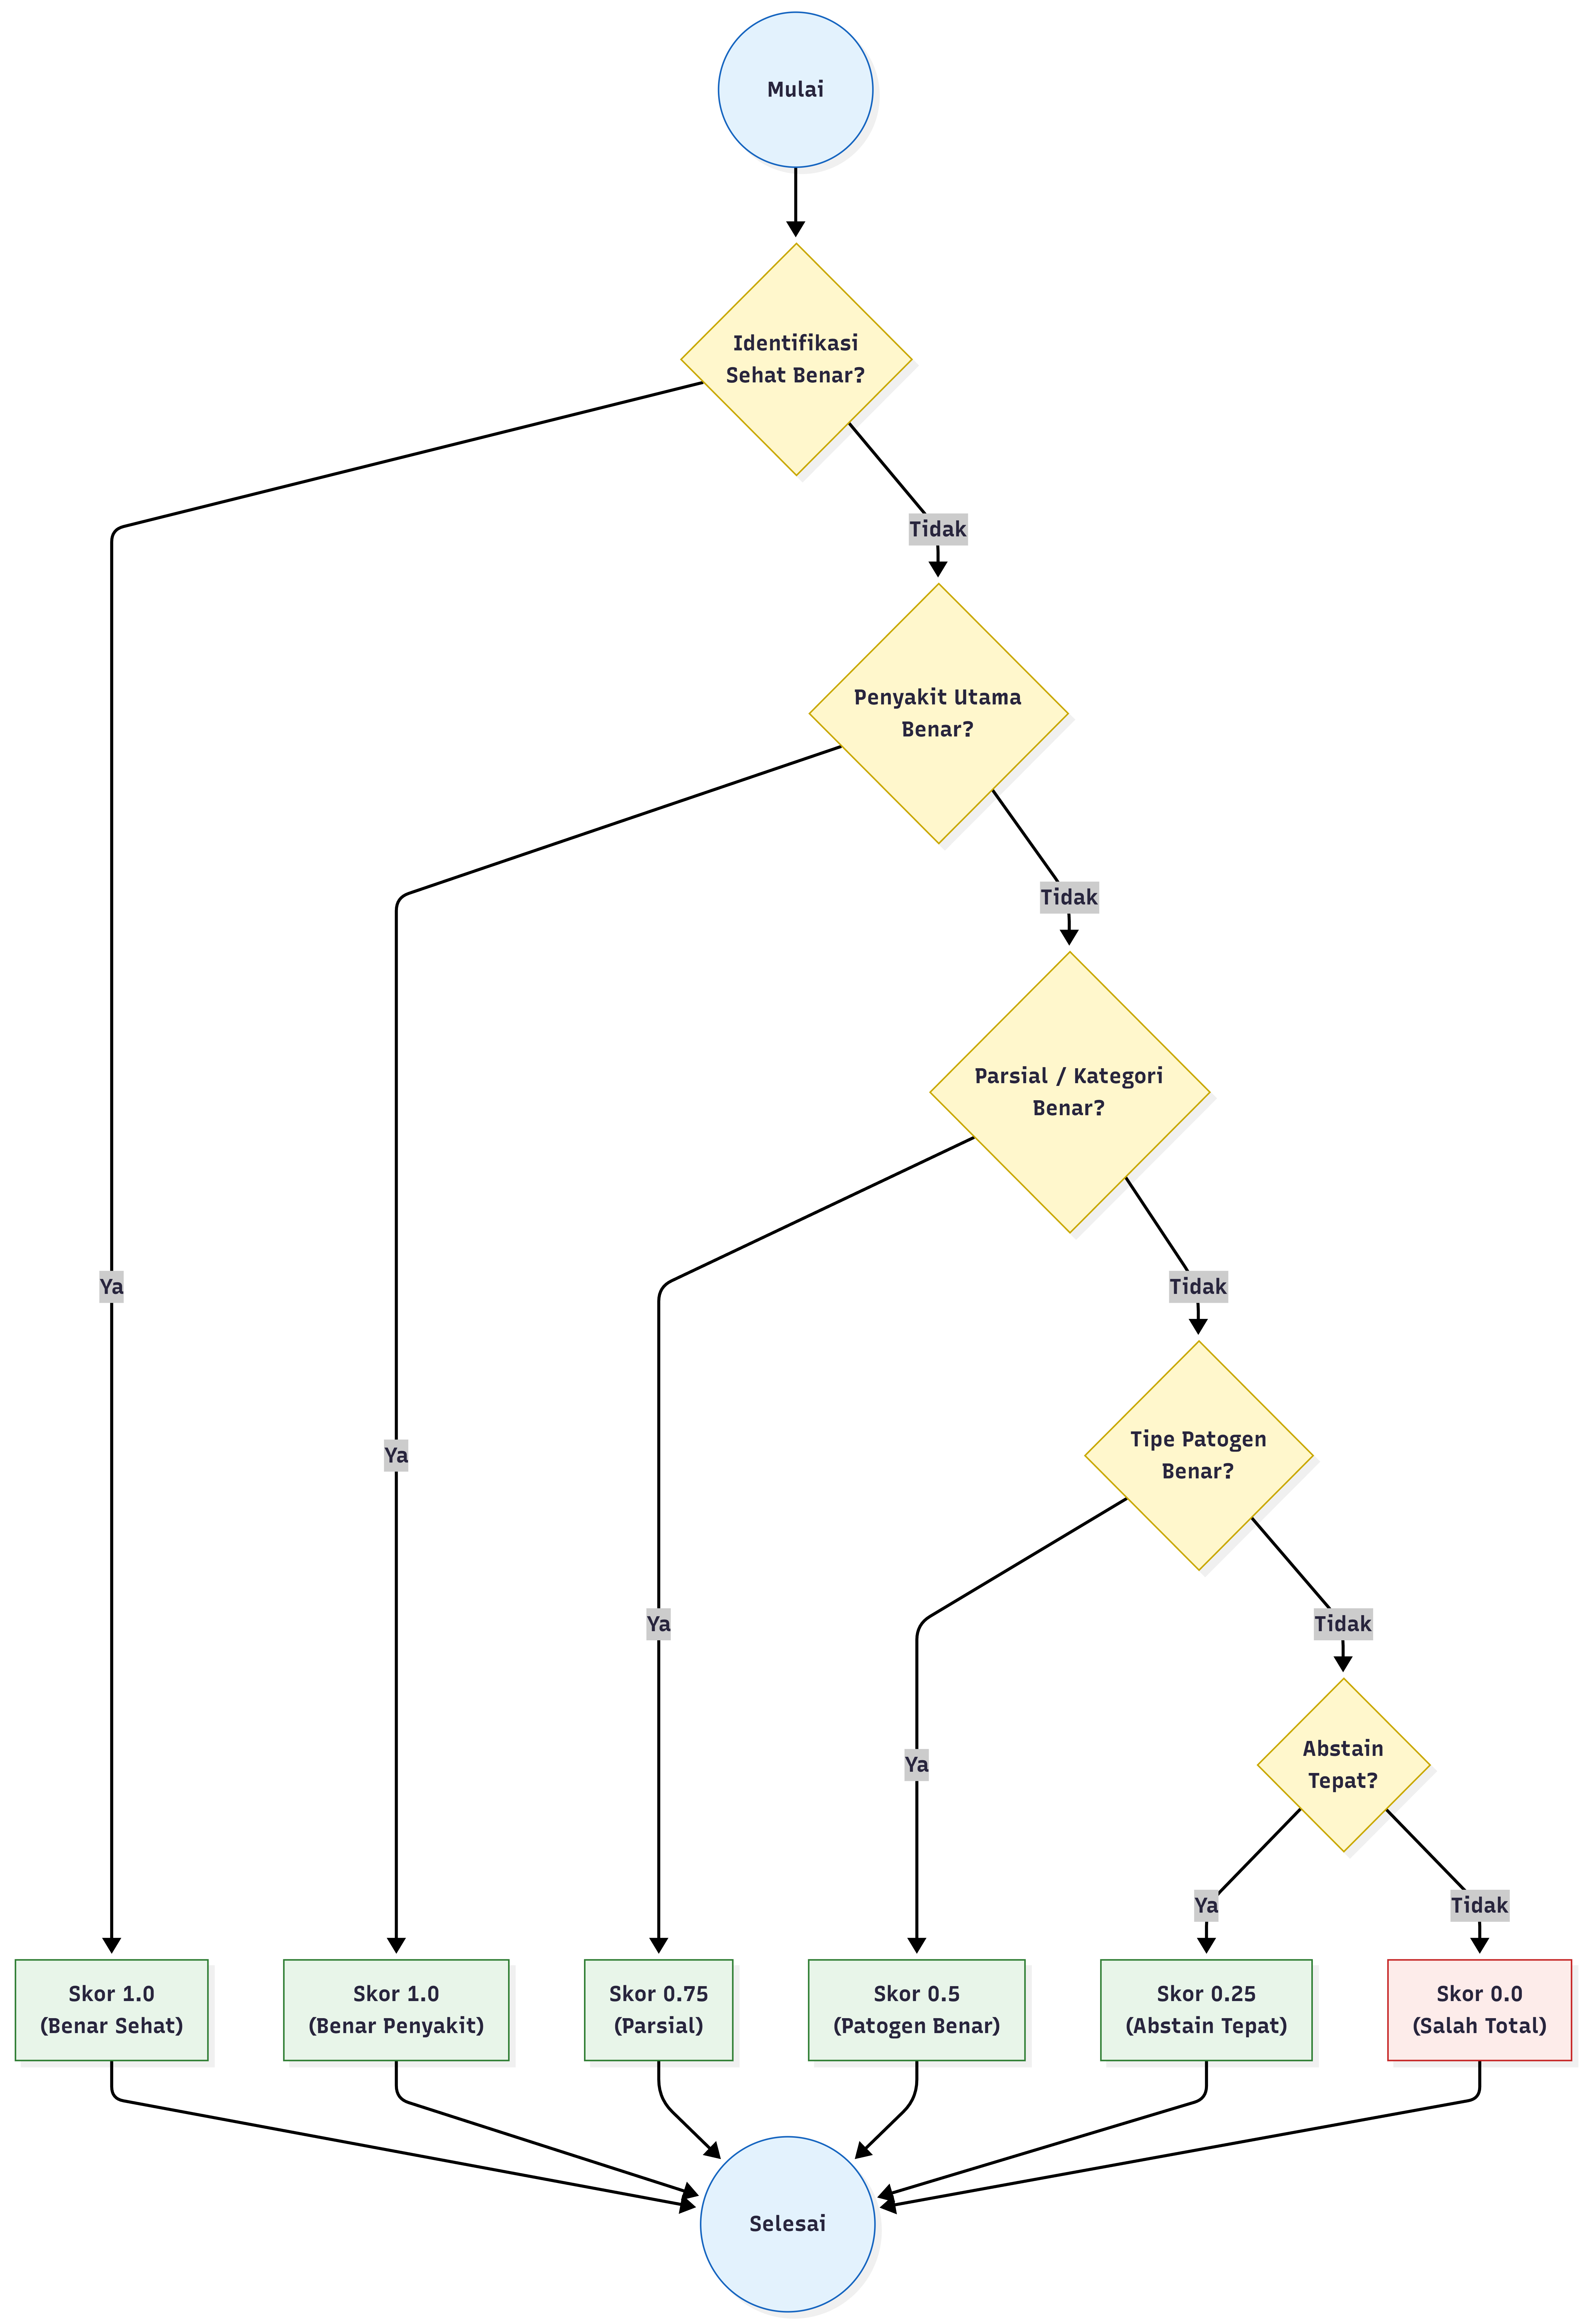
\includegraphics[width=0.6\textwidth]{bab3/dagtree.png}
    \caption{Diagram Alur Logika Evaluasi Disease Accuracy menggunakan DAG}
    \label{fig:disease_accuracy_dag}
\end{figure}

\paragraph{Trajectory Accuracy}
\textit{Trajectory Accuracy} ($M_{ta}$) adalah metrik evaluasi yang dirancang untuk mengukur efisiensi dan ketepatan urutan pengambilan keputusan (\textit{trajectory}) oleh agen dalam menyelesaikan tugas. Evaluasi ini menggunakan pendekatan \textit{LLM-as-a-judge}, di mana LLM bertindak sebagai penilai kualitatif yang memvalidasi keputusan agen terhadap rubrik yang telah ditentukan. Pendekatan ini diterapkan karena mekanisme kerja sistem agentik yang kompleks, yang melibatkan mekanisme cadangan (\textit{fallback}) pada modul deteksi objek maupun pencarian informasi yang bergantung pada konteks situasi.

Metrik ini dirancang menggunakan kerangka kerja AgentEval dari LangSmith. Penilaian dilakukan dengan membandingkan trajektori aktual agen terhadap trajektori referensi menggunakan prinsip \textit{superset} dan kesesuaian semantik. Prinsip \textit{superset} mengizinkan agen untuk memanggil alat tambahan yang relevan (misalnya, alat deteksi tambahan untuk validasi) selama seluruh alat kunci yang terdapat dalam referensi telah dipenuhi. Sementara itu, prinsip kesesuaian semantik memungkinkan evaluator untuk memvalidasi penggunaan alat yang berbeda namun memiliki fungsi yang setara, seperti penggunaan pencarian web (\textit{web\_search}) untuk menggantikan pencarian basis pengetahuan (\textit{knowledgebase\_search}) apabila informasi internal tidak memadai. Tabel \ref{tab:trajectory_data_requirements} menyajikan kebutuhan data untuk menjalankan evaluasi \textit{Trajectory Accuracy}.

\begin{table}[H]
    \centering
    \caption{Kebutuhan Data untuk Evaluasi Trajectory Accuracy}
    \label{tab:trajectory_data_requirements}
    \small
    \resizebox{\textwidth}{!}{
    \begin{tabular}{|l|l|p{8cm}|}
    \hline
    \textbf{Kategori} & \textbf{Parameter} & \textbf{Deskripsi} \\ \hline
    \multirow{2}{*}{\textbf{Input}} & \textit{user\_text} & Instruksi atau pertanyaan teks dari pengguna. \\ \cline{2-3} 
     & \textit{image\_url} & Tautan citra tanaman yang menjadi konteks visual analisis. \\ \hline
    \textbf{Aktual} & \textit{trace\_messages} & Riwayat lengkap langkah eksekusi (\textit{trace}) dan pemanggilan alat oleh agen. \\ \hline
    \textbf{Referensi} & \textit{reference\_tool\_calls} & Daftar alat yang diharapkan dipanggil untuk menyelesaikan tugas secara optimal (Standar Emas). \\ \hline
    \end{tabular}
    }
\end{table}

Evaluasi dilakukan dengan memberikan instruksi (\textit{prompt}) spesifik kepada LLM penilai yang mencakup prinsip desain agen, aturan semantik, dan rubrik penilaian. Model Gemini 2.5 Pro digunakan sebagai evaluator untuk memastikan kemampuan penalaran yang tinggi dalam menilai konteks trajektori. Rangkuman logika evaluasi dan rubrik penilaian disajikan pada Tabel \ref{tab:trajectory_rubric}.

\begin{table}[H]
    \centering
    \caption{Logika Evaluasi dan Rubrik Penilaian Trajectory Accuracy}
    \label{tab:trajectory_rubric}
    \small
    \resizebox{\textwidth}{!}{
    \begin{tabular}{|p{3cm}|p{2.5cm}|p{7.5cm}|}
    \hline
    \textbf{Komponen} & \textbf{Elemen} & \textbf{Deskripsi} \\ \hline
    \multirow{2}{*}{\textbf{Prinsip Desain}} & Alur Kerja & Identifikasi visual diprioritaskan, diikuti deteksi opsional, dan pencarian pengetahuan jika pengguna membutuhkan panduan pengobatan. \\ \cline{2-3}
    & Fallback & Pengalihan ke pencarian jika kepercayaan visual rendah. \\ \hline
    \multirow{2}{*}{\textbf{Aturan Semantik}} & Superset & Agen boleh memanggil alat tambahan (misal: deteksi ekstra) selama alat wajib terpenuhi. \\ \cline{2-3}
    & Substitusi & \textit{knowledgebase\_search} dan \textit{web\_search} dianggap setara sebagai alat pencarian informasi. \\ \hline
    \multirow{5}{*}{\textbf{Rubrik Skor}} & 0.0 & Alat kritis referensi tidak dipanggil sama sekali. \\ \cline{2-3}
    & 0.2 & Kehilangan beberapa alat kunci penting. \\ \cline{2-3}
    & 0.5 & Alat wajib lengkap, namun terdapat langkah tambahan yang tidak logis atau berlebihan. \\ \cline{2-3}
    & 0.75 & \textit{Superset} valid dengan inefisiensi minor (misal: urutan kurang optimal). \\ \cline{2-3}
    & 1.0 & \textit{Superset} sempurna; semua alat wajib ada, langkah tambahan beralasan kuat, dan alur logis. \\ \hline
    \end{tabular}
    }
\end{table}

Skor akhir yang dihasilkan berupa nilai numerik diskrit (0.0, 0.2, 0.5, 0.75, atau 1.0) yang merepresentasikan kualitas trajektori agen dalam mencapai solusi yang efisien dan logis.

\paragraph{Agent Goal Accuracy}
\textit{Agent Goal Accuracy} ($M_{aga}$) adalah metrik kustom yang digunakan untuk mengevaluasi eksekusi agen dan menentukan apakah tujuan tingkat tinggi (\textit{high-level goal}) telah tercapai. Berbeda dengan \textit{Trajectory Accuracy} yang lebih menitikberatkan pada validitas urutan pemanggilan alat, metrik ini mengevaluasi pencapaian tujuan secara komprehensif dengan mempertimbangkan masukan pengguna, konteks pemanggilan alat, serta kualitas jawaban akhir. Penilaian dilakukan dengan membandingkan hasil aktual terhadap tujuan referensi yang merepresentasikan hasil ideal dari interaksi.

Metrik ini dirancang menggunakan kerangka kerja G-Eval yang diusulkan oleh \textcite{liuGEvalNLGEvaluation2023} melalui pustaka DeepEval. G-Eval digunakan untuk mengurangi subjektivitas dari evaluator tradisional dengan memanfaatkan LLM (Gemini 2.5 Pro) sebagai penilai yang mengikuti kriteria evaluasi terstruktur (\textit{LLM-as-a-judge}).

Kebutuhan data untuk evaluasi \textit{Agent Goal Accuracy} dirinci pada Tabel \ref{tab:goal_accuracy_data}.

\begin{table}[H]
    \centering
    \caption{Kebutuhan Data untuk Evaluasi Agent Goal Accuracy}
    \label{tab:goal_accuracy_data}
    \small
    \resizebox{\textwidth}{!}{
    \begin{tabular}{|l|l|p{8cm}|}
    \hline
    \textbf{Kategori} & \textbf{Parameter} & \textbf{Deskripsi} \\ \hline
    \multirow{2}{*}{\textbf{Input}} & \textit{user\_text} & Instruksi atau pertanyaan teks dari pengguna. \\ \cline{2-3} 
     & \textit{image\_url} & Tautan citra masukan (multimodal). \\ \hline
    \multirow{2}{*}{\textbf{Aktual}} & \textit{final\_answer} & Jawaban akhir yang dihasilkan oleh agen. \\ \cline{2-3}
     & \textit{tools\_called} & Daftar alat yang dipanggil agen beserta keluarannya. \\ \hline
    \textbf{Referensi} & \textit{reference\_goal} & Tujuan referensi yang diharapkan (misal: identifikasi, panduan, atau penolakan). \\ \hline
    \end{tabular}
    }
\end{table}

Desain evaluator ini mencakup kriteria, langkah evaluasi, dan rubrik penilaian yang dirangkum pada Tabel \ref{tab:goal_evaluator_design}.

\begin{table}[H]
    \centering
    \caption{Desain Evaluator Agent Goal Accuracy}
    \label{tab:goal_evaluator_design}
    \small
    \resizebox{\textwidth}{!}{
    \begin{tabular}{|l|p{10cm}|}
    \hline
    \textbf{Komponen} & \textbf{Rincian} \\ \hline
    \textbf{Kriteria} & Evaluasi keberhasilan agen mencapai \textit{reference\_goal} berdasarkan output aktual dan penggunaan alat. Penilaian mencakup aspek identifikasi penyakit, panduan manajemen, analisis gejala, ekspresi ketidakpastian, dan penolakan permintaan di luar jangkauan. \\ \hline
    \textbf{Langkah Evaluasi} & \begin{enumerate}[nosep, leftmargin=*]
        \item Ekstrak tujuan referensi dari data yang diharapkan.
        \item Identifikasi tujuan utama (identifikasi, pengobatan, atau penolakan).
        \item Periksa alat yang dipanggil dan outputnya.
        \item Verifikasi observasi visual agen (jika gambar tersedia).
        \item Evaluasi kualitas dan kelengkapan pemenuhan tujuan dalam respon akhir.
    \end{enumerate} \\ \hline
    \textbf{Rubrik} & \begin{itemize}[nosep, leftmargin=*]
        \item \textbf{0--1 (Tidak Ada)}: Agen gagal menangani tujuan atau melenceng sepenuhnya.
        \item \textbf{2--4 (Minimal)}: Mencoba mencapai tujuan tetapi dengan celah signifikan atau penggunaan alat yang buruk.
        \item \textbf{5--8 (Parsial)}: Menangani tujuan utama tetapi melewatkan komponen kunci atau kurang mendalam.
        \item \textbf{9--10 (Penuh)}: Sepenuhnya memenuhi tujuan referensi dengan kualitas tinggi dan penggunaan alat yang tepat.
    \end{itemize} \\ \hline
    \end{tabular}
    }
\end{table}

Skor yang dihasilkan oleh evaluator G-Eval dinormalisasi ke dalam rentang 0.0 hingga 1.0, di mana nilai 1.0 menunjukkan pencapaian tujuan yang sempurna sesuai referensi.

\paragraph{Faithfulness}
\textit{Faithfulness} ($M_{fth}$) merupakan metrik evaluasi kustom yang mengadopsi pendekatan \textit{LLM-as-a-judge} menggunakan kerangka kerja G-Eval dari pustaka DeepEval. Metrik ini berfungsi untuk mengevaluasi integritas faktual dari respons agen, memastikan bahwa jawaban akhir (\textit{final answer}) yang dihasilkan selaras dengan konteks informasi yang diperoleh dari seluruh alat (\textit{retrieved context}). Evaluasi ini krusial untuk mendeteksi halusinasi, yaitu kondisi di mana model menghasilkan informasi yang tampak meyakinkan namun tidak didukung oleh bukti data internal maupun eksternal yang diakses.

Berbeda dengan implementasi standar, metrik ini dirancang khusus untuk mengakomodasi sifat multimodal dan pengetahuan domain agen. Dalam desain ini, observasi visual yang dilakukan agen terhadap citra tanaman serta pemberian saran perawatan umum yang bersifat standar (\textit{best practices}) diakui sebagai informasi valid yang tidak memerlukan sitasi dari alat pencarian, selama masih dalam batas kewajaran domain.

Tabel \ref{tab:faithfulness_data_requirements} menyajikan komponen data yang digunakan dalam proses evaluasi.

\begin{table}[H]
    \centering
    \caption{Kebutuhan Data untuk Evaluasi Faithfulness}
    \label{tab:faithfulness_data_requirements}
    \small
    \resizebox{\textwidth}{!}{
    \begin{tabular}{|l|l|p{8cm}|}
    \hline
    \textbf{Kategori} & \textbf{Parameter} & \textbf{Deskripsi} \\ \hline
    \multirow{2}{*}{\textbf{Input}} & \textit{user\_text} & Pertanyaan atau instruksi teks dari pengguna. \\ \cline{2-3} 
     & \textit{image\_url} & Tautan citra tanaman sebagai dasar validasi observasi visual agen. \\ \hline
    \multirow{2}{*}{\textbf{Aktual}} & \textit{final\_answer} & Jawaban akhir yang dihasilkan oleh agen. \\ \cline{2-3}
     & \textit{retrieval\_context} & Kumpulan potongan informasi teks yang diekstraksi dari keluaran seluruh alat (pencarian, deteksi, dan klasifikasi). \\ \hline
    \end{tabular}
    }
\end{table}

Desain evaluator \textit{Faithfulness} mencakup kriteria penilaian yang spesifik terhadap perilaku agen serta rubrik penilaian bertingkat. Rincian desain ini dirangkum pada Tabel \ref{tab:faithfulness_evaluator_design}.

\begin{table}[H]
    \centering
    \caption{Desain Evaluator Faithfulness}
    \label{tab:faithfulness_evaluator_design}
    \small
    \resizebox{\textwidth}{!}{
    \begin{tabular}{|l|p{10cm}|}
    \hline
    \textbf{Komponen} & \textbf{Rincian} \\ \hline
    \textbf{Kriteria} & Evaluasi kesetiaan (\textit{faithfulness}) respons terhadap bukti dengan mempertimbangkan kapabilitas agen: \newline
    1. \textbf{Observasi Visual}: Agen HARUS melakukan observasi dari gambar (valid tanpa pencarian). \newline
    2. \textbf{Saran Umum}: Agen DAPAT memberikan praktik terbaik umum (sanitasi, isolasi) tanpa pencarian. \newline
    3. \textbf{Klaim Spesifik}: Identifikasi penyakit, nama patogen, dan pengobatan kimiawi HARUS didasarkan pada \textit{retrieval\_context}. \newline
    4. \textbf{Ketidakpastian}: Agen HARUS menyatakan ketidakpastian jika bukti terbatas. \\ \hline
    \textbf{Langkah Evaluasi} & \begin{enumerate}[nosep, leftmargin=*]
        \item Identifikasi observasi visual dan rekomendasi umum dalam output.
        \item Identifikasi semua klaim spesifik penyakit (nama, biologi, kimia).
        \item Verifikasi apakah observasi visual masuk akal terhadap citra.
        \item Periksa apakah setiap klaim spesifik didukung oleh konteks pencarian.
        \item Hitung proporsi klaim yang tidak didukung atau difabrikasi.
    \end{enumerate} \\ \hline
    \textbf{Rubrik} & \begin{itemize}[nosep, leftmargin=*]
        \item \textbf{0.0--0.2 (Tidak Setia)}: Informasi didominasi fabrikasi; rekomendasi spesifik dikarang tanpa dasar.
        \item \textbf{0.3--0.4 (Sebagian Besar Tidak Setia)}: Banyak klaim spesifik tidak didukung bukti.
        \item \textbf{0.5--0.6 (Setia Sebagian)}: Beberapa klaim kurang dukungan atau spekulasi disajikan sebagai fakta.
        \item \textbf{0.7--0.8 (Sebagian Besar Setia)}: Klaim inti didasarkan bukti, hanya detail minor yang terlewat.
        \item \textbf{0.9--1.0 (Sangat Setia)}: Seluruh klaim spesifik didukung bukti; observasi visual dan saran umum tepat.
    \end{itemize} \\ \hline
    \end{tabular}
    }
\end{table}

Skor akhir yang dihasilkan oleh evaluator direpresentasikan dalam nilai kontinu antara 0.0 hingga 1.0, di mana nilai yang lebih tinggi mengindikasikan tingkat kepatuhan fakta yang lebih baik terhadap sumber data.

\paragraph{Context Relevance}
\textit{Context Relevance} ($M_{cr}$) merupakan metrik yang diadopsi dari kerangka kerja RAGAS untuk mengevaluasi seberapa relevan potongan informasi (\textit{retrieved contexts}) yang diambil oleh sistem terhadap masukan pengguna (\textit{user input}). Evaluasi ini dilakukan menggunakan mekanisme \textit{LLM-as-a-judge} yang melibatkan dua pemanggilan \textit{prompt} penilaian secara independen untuk mengurangi bias model. Setiap \textit{prompt} menginstruksikan model evaluator untuk memberikan penilaian relevansi pada skala diskret 0 hingga 2. Nilai 0 mengindikasikan bahwa konteks yang diambil sama sekali tidak relevan dengan kueri, nilai 1 menunjukkan relevansi sebagian, dan nilai 2 menandakan bahwa konteks sepenuhnya relevan. Skor dari kedua penilaian tersebut kemudian dinormalisasi ke dalam rentang [0,1] dan dirata-ratakan untuk menghasilkan skor akhir. Skor yang lebih tinggi merepresentasikan keselarasan yang lebih baik antara konteks informasi yang ditemukan dengan kebutuhan pengguna.

Metrik ini berbeda dengan pendekatan \textit{Context Relevance} awal yang diperkenalkan pada makalah RAGAS oleh \textcite{esRagasAutomatedEvaluation2025}, yang mendefinisikan relevansi berdasarkan rasio ekstraksi tingkat kalimat (jumlah kalimat relevan dibagi total kalimat). Implementasi pada penelitian ini menggunakan pendekatan penilaian diskret (\textit{discrete rating}) yang dinilai lebih \textit{robust} dan efisien. Pendekatan ini mengurangi kerentanan terhadap kesalahan pemisahan kalimat (\textit{sentence boundary errors}) yang sering terjadi pada teks teknis, serta lebih hemat biaya komputasi (\textit{overhead}) sambil tetap mempertahankan tujuan inti evaluasi. Selain itu, implementasi metrik ini telah disesuaikan untuk mendukung input multimodal, di mana konteks visual dari citra turut diperhitungkan dalam formulasi pertanyaan pengguna yang disajikan ke evaluator.

Sebagai ilustrasi perhitungan, misalkan pengguna bertanya "Apa obat untuk penyakit bercak daun ini?" dan sistem mengambil dua konteks: (1) "Bercak daun Cercospora dapat dikendalikan dengan fungisida berbahan aktif mankozeb" dan (2) "Sanitasi lahan penting untuk mencegah penyebaran". Karena kedua konteks tersebut secara kolektif menjawab pertanyaan pengguna (memberikan solusi obat dan pencegahan), kedua \textit{prompt} evaluator akan memberikan skor 2 (sepenuhnya relevan). Skor ini kemudian dinormalisasi ($2/2 = 1.0$) dan dirata-ratakan, menghasilkan skor akhir \textit{Context Relevance} sebesar 1.0.

Kebutuhan data untuk menjalankan evaluasi \textit{Context Relevance} dirangkum pada Tabel \ref{tab:context_relevance_data}.

\begin{table}[H]
    \centering
    \caption{Kebutuhan Data untuk Evaluasi Context Relevance}
    \label{tab:context_relevance_data}
    \small
    \resizebox{\textwidth}{!}{
    \begin{tabular}{|l|l|p{8cm}|}
    \hline
    \textbf{Kategori} & \textbf{Parameter} & \textbf{Deskripsi} \\ \hline
    \multirow{2}{*}{\textbf{Input}} & \textit{user\_text} & Teks pertanyaan atau instruksi dari pengguna. \\ \cline{2-3} 
     & \textit{image\_url} & Tautan citra tanaman. Jika tersedia, indikator visual ditambahkan ke \textit{prompt} evaluator untuk konteks. \\ \hline
    \textbf{Aktual} & \textit{retrieved\_contexts} & Daftar potongan teks yang diekstraksi dari riwayat pemanggilan alat (\textit{trace}), mencakup hasil pencarian dokumen maupun deteksi. \\ \hline
    \end{tabular}
    }
\end{table}

\subsubsection{Evaluasi Pengujian Multi-Tahap}
Evaluasi kinerja agen pada pengujian ini dilakukan menggunakan metrik kustom bernama \textit{Domain Adherence} ($M_{dad}$). Metrik ini merupakan implementasi dari pendekatan \textit{LLM-as-a-judge} yang dibangun menggunakan pustaka OpenEval dari LangSmith. Metrik ini bersifat juga \textit{self-explaining}, di mana evaluator tidak hanya memberikan skor penilaian tetapi juga menyertakan alasan kualitatif yang mendasari skor tersebut.

Evaluator bekerja dengan menganalisis riwayat percakapan lengkap (\textit{trajectory}) antara agen dan pengguna simulasi. Penilaian dilakukan berdasarkan instruksi (\textit{prompt}) evaluasi yang menginstruksikan model juri untuk memberikan skor tinggi jika agen berhasil menjawab pertanyaan terkait tanaman dan menolak permintaan di luar domain secara sopan. Sebaliknya, skor rendah diberikan jika agen gagal mempertahankan batasan domainnya. \textit{Prompt} yang digunakan oleh evaluator dalam metrik ini disajikan pada Gambar \ref{fig:prompt_domain_adherence}.

\begin{figure}[H]
    \centering
    \includegraphics[width=1\textwidth]{bab3/promptdomainadherence.png}
    \caption{\textit{Prompt} Evaluasi untuk Metrik Domain Adherence}
    \label{fig:prompt_domain_adherence}
\end{figure}

\section{Penyampaian Hasil}
Hasil penelitian yang telah dilaksanakan dianalisis dan dibahas dalam bentuk laporan tertulis berupa skripsi. Laporan ini mencakup perancangan arsitektur sistem agentik, implementasi teknis, serta hasil evaluasi kinerja sistem menggunakan pendekatan \textit{LLM-as-a-judge}. Pembahasan dalam laporan meliputi integrasi model deteksi objek tanaman menggunakan YOLOv11 dan OWLv2, modul pencarian multimodal berbasis SCOLD, serta pengembangan agen cerdas dengan pola ReAct yang memanfaatkan mekanisme \textit{Retrieval-Augmented Generation} (RAG). Laporan ini diharapkan dapat memberikan kontribusi terhadap pengembangan teknologi identifikasi penyakit tanaman yang lebih adaptif dan fleksibel. Selain itu, penelitian ini juga dapat menjadi rujukan dalam penerapan teknologi sistem agentik dan kecerdasan buatan multimodal di bidang pertanian untuk membantu pengelolaan kesehatan tanaman.
\chapter{HASIL DAN PEMBAHASAN}

\section{Hasil Perancangan dan Pengembangan Sistem Agentik}
Implementasi sistem agentik telah berhasil direalisasikan menggunakan kerangka kerja LangChain dan pustaka LangGraph sesuai dengan rancangan arsitektur yang telah dibahas sebelumnya. Sistem ini memodelkan perilaku agen LLM dalam struktur graf berstatus (\textit{stateful graph}) untuk menangani tugas identifikasi penyakit tanaman secara adaptif.

Hasil kompilasi dari definisi graf agen disajikan pada Gambar \ref{fig:compiled_state_graph}. Representasi ini menunjukkan struktur topologi graf yang terbentuk setelah kode program dieksekusi. Simpul-simpul utama yang merepresentasikan logika pengambilan keputusan (agen) dan eksekusi tindakan (alat) telah terbentuk dan terhubung oleh sisi-sisi (\textit{edges}) yang mengatur aliran kontrol. Struktur ini memvalidasi bahwa desain pola \textit{Reasoning and Acting} (ReAct) telah berhasil diterjemahkan ke dalam objek eksekutif yang siap dijalankan.

\begin{figure}[H]
    \centering
    \includegraphics[width=0.4\textwidth]{bab4/compiledstategraph.png}
    \caption{Representasi graf sistem agentik setelah proses kompilasi}
    \label{fig:compiled_state_graph}
\end{figure}

Verifikasi lebih lanjut terhadap struktur dan alur kerja agen dilakukan menggunakan platform LangSmith. Gambar \ref{fig:agent_graph_langsmith} menampilkan visualisasi graf agen dalam lingkungan LangSmith Studio. Visualisasi ini memberikan gambaran yang lebih interaktif mengenai bagaimana agen berpindah dari satu status ke status lainnya, mulai dari inisialisasi, evaluasi model, pemanggilan alat, hingga terminasi proses. Kesesuaian antara graf yang dirancang dan visualisasi ini mengonfirmasi integritas implementasi alur kerja sistem.

\begin{figure}[H]
    \centering
    \includegraphics[width=1\textwidth]{bab4/agentgraphdilangsmithstudio.png}
    \caption{Visualisasi graf agen pada LangSmith Studio}
    \label{fig:agent_graph_langsmith}
\end{figure}

Pengujian fungsionalitas dasar sistem dilakukan dengan memberikan masukan berupa citra daun yang bergejala penyakit disertai instruksi teks. Hasil keluaran dari pengujian ini ditunjukkan pada Gambar \ref{fig:agent_output_langsmith}. Sistem terbukti mampu menerima masukan multimodal, memprosesnya melalui alur kerja agen, dan menghasilkan respons akhir yang relevan terhadap permintaan pengguna. Keberhasilan ini menunjukkan bahwa mekanisme integrasi antara model bahasa dan antarmuka input-output telah berjalan dengan baik.

\begin{figure}[H]
    \centering
    \includegraphics[width=1\textwidth]{bab4/contohoutputagentdilangsmithstudio.png}
    \caption{Contoh keluaran agen saat diuji di LangSmith Studio}
    \label{fig:agent_output_langsmith}
\end{figure}

Untuk memvalidasi proses penalaran dan penggunaan alat oleh agen, dilakukan analisis terhadap jejak eksekusi (\textit{trace}) yang direkam oleh LangSmith. Gambar \ref{fig:agent_trace_langsmith} memperlihatkan rincian langkah-langkah yang diambil agen dalam menyelesaikan tugas. Jejak tersebut menampilkan urutan pemanggilan alat yang dilakukan oleh agen berdasarkan analisis konteks, serta respons yang diterima dari alat tersebut. Transparansi ini membuktikan bahwa agen tidak hanya memberikan jawaban, tetapi juga melakukan proses penalaran dan pengambilan tindakan yang logis sesuai dengan pola ReAct yang diterapkan.

\begin{figure}[H]
    \centering
    \includegraphics[width=1\textwidth]{bab4/contohtracedilangsmithstudio.png}
    \caption{Jejak eksekusi (\textit{trace}) agen yang menampilkan pemanggilan alat}
    \label{fig:agent_trace_langsmith}
\end{figure}

\section{Hasil Perancangan dan Pengembangan Agen LLM}
Pengembangan agen LLM difokuskan pada implementasi instruksi sistem (\textit{system instructions}) dan konfigurasi model untuk memastikan perilaku agen sesuai dengan parameter yang telah dirancang. Implementasi ini mencakup manajemen prompt menggunakan LangSmith Prompt Hub serta realisasi kerangka kerja CO-STAR.

Manajemen instruksi dilakukan secara terpusat menggunakan layanan LangSmith Prompt Hub. Pendekatan ini memisahkan logika kode program dengan konfigurasi instruksi bahasa alami, yang memungkinkan proses iterasi dan pembaruan instruksi dilakukan tanpa mengubah kode sumber aplikasi secara langsung. Gambar \ref{fig:langsmith_prompt_hub} menampilkan antarmuka manajemen prompt yang digunakan, di mana versi prompt dikelola dan dilacak perubahannya.

\begin{figure}[H]
    \centering
    \includegraphics[width=1\textwidth]{bab4/tampilanpromptdilangsmithprompthub.png}
    \caption{Tampilan antarmuka manajemen prompt pada LangSmith Prompt Hub}
    \label{fig:langsmith_prompt_hub}
\end{figure}
Kerangka kerja CO-STAR yang dirancang pada tahap sebelumnya telah diterjemahkan menjadi blok instruksi terstruktur. Bagian \textit{Context} menetapkan peran agen sebagai ahli patologi tanaman dengan batasan domain yang ketat, sedangkan bagian \textit{Objective} menekankan pada jawaban yang berbasis bukti (\textit{evidence-grounded}). Cuplikan implementasi instruksi bagian Context dan Objective disajikan dalam Gambar \ref{fig:prompt_context}.

\begin{figure}[H]
    \centering
    \includegraphics[width=1\textwidth]{bab4/contextobjective.png}
    \caption{Realisasi instruksi Context dan Objective pada sistem}
    \label{fig:prompt_context}
\end{figure}

Selanjutnya, komponen \textit{Style}, \textit{Tone}, dan \textit{Audience} mendefinisikan persona agen dalam berinteraksi. Agen diinstruksikan untuk selalu menyesuaikan bahasa dengan pengguna (misalnya Bahasa Indonesia), membedakan secara tegas antara observasi visual dan inferensi, serta mempertahankan nada yang tenang dan jujur mengenai ketidakpastian. Target audiens yang bervariasi dari pemilik tanaman hingga profesional pertanian menuntut penjelasan yang jelas tanpa jargon berlebih. Implementasi ketiga komponen ini ditampilkan pada Gambar \ref{fig:prompt_sta}.

\begin{figure}[H]
    \centering
    \includegraphics[width=1\textwidth]{bab4/styletoneaudience.png}
    \caption{Realisasi instruksi Style, Tone, dan Audience pada sistem}
    \label{fig:prompt_sta}
\end{figure}

Terakhir, komponen \textit{Response} menetapkan struktur standar untuk jawaban identifikasi yang mewajibkan penggunaan observasi visual, integrasi konteks, hingga identifikasi dengan penalaran. Struktur ini juga mencakup mekanisme tindak lanjut (\textit{follow-up}) jika data kurang mencukupi serta batasan ketat mengenai apa yang tidak boleh disertakan seperti resep kimia atau saran medis. Detail instruksi struktur respons disajikan pada Gambar \ref{fig:prompt_response}.

\begin{figure}[H]
    \centering
    \includegraphics[width=1\textwidth]{bab4/response.png}
    \caption{Realisasi instruksi Response Structure pada sistem}
    \label{fig:prompt_response}
\end{figure}


Agar agen dapat berinteraksi dengan alat yang disediakan dengan biak, instruksi sistem juga menyertakan referensi teknis mengenai alat-alat yang tersedia (\textit{Tools Reference}). Bagian ini memberikan spesifikasi formal untuk fungsi seperti \texttt{web\_search} dan \texttt{knowledgebase\_search} dalam modul pencarian informasi, mencakup parameter, tujuan, dan contoh penggunaannya. Referensi ini memastikan agen dapat menyusun pemanggilan alat yang valid secara sintaksis dan semantik. Contoh referensi penggunaan alat tersebut ditampilkan pada Gambar \ref{fig:prompt_tools}.

\begin{figure}[H]
    \centering
    \includegraphics[width=1\textwidth]{bab4/referensitool.png}
    \caption{Realisasi referensi teknis alat pada sistem}
    \label{fig:prompt_tools}
\end{figure}

Agen juga dilengkapi dengan kebijakan penggunaan alat (\textit{Tool Decision Policy}) yang dirancang untuk mengoptimalkan akurasi dan efisiensi biaya. Kebijakan ini mengatur alur pengambilan keputusan agen mulai dari validasi kualitas citra, pemilihan strategi deteksi (apakah menggunakan deteksi objek atau klasifikasi langsung), hingga mekanisme validasi hasil dan tindakan pemulihan (\textit{fallback}) jika terjadi inkonsistensi. Selain itu, aturan keselamatan (\textit{Safety Rules}) diterapkan untuk mencegah halusinasi, seperti kewajiban melakukan validasi visual sebelum memanggil alat deteksi dan larangan memberikan saran medis tanpa rujukan. Alur logika keputusan ini divisualisasikan dalam diagram alir pada Gambar \ref{fig:tool_decision_flowchart}.

\begin{figure}[H]
    \centering
    \resizebox{0.5\textwidth}{!}{%
    \begin{tikzpicture}[
        node distance=0.8cm,
        font=\small,
        start/.style={circle, draw, fill=blue!10, minimum size=1cm, align=center},
        stop/.style={ellipse, draw, fill=green!10, minimum height=1cm, align=center},
        process/.style={rectangle, draw, fill=white, minimum width=3cm, minimum height=0.8cm, align=center, text width=3cm},
        decision/.style={rounded rectangle, draw, fill=blue!10, minimum width=2.5cm, minimum height=0.8cm, align=center, text width=2.5cm},
        arrow/.style={-stealth, thick}
    ]

        % Nodes
        \node [start] (start) {Mulai: Input Pengguna};
        \node [decision, below=of start] (quality) {Kualitas Citra Baik?};
        \node [process, right=1.2cm of quality] (reject) {Minta Foto Ulang};
        
        \node [decision, below=1.2cm of quality] (strategy) {Perlu Deteksi Objek?};
        \node [process, left=1.2cm of strategy] (full) {Mode \textit{Full-Image}};
        \node [process, below=1.2cm of strategy] (detect) {Deteksi \textit{Closed-Set}};
        
        \node [decision, below=1.2cm of detect] (valid) {Deteksi Valid?};
        \node [process, right=1.2cm of valid] (open) {Deteksi \textit{Open-Vocab}};
        
        \node [process, below=1.2cm of valid] (ident) {Identifikasi Penyakit};
        
        \node [decision, below=1.2cm of ident] (reliable) {Hasil Konsisten?};
        \node [process, right=1.2cm of reliable] (fallback) {Fallback: Ganti Metode/KB};
        
        \node [decision, below=1.2cm of reliable] (guide) {Butuh Panduan?};
        \node [process, left=1.2cm of guide] (kb) {Pencarian KB/Web};
        
        \node [stop, below=of guide] (end) {Selesai: Respons Akhir};

        % Edges
        \draw [arrow] (start) -- (quality);
        \draw [arrow] (quality) -- node[above] {Tidak} (reject);
        \draw [arrow] (quality) -- node[right] {Ya} (strategy);
        
        \draw [arrow] (strategy) -- node[above] {Tidak} (full);
        \draw [arrow] (strategy) -- node[right] {Ya} (detect);
        
        \draw [arrow] (detect) -- (valid);
        \draw [arrow] (valid) -- node[right] {Ya} (ident);
        \draw [arrow] (valid) -| node[above, near start] {Tidak} (full);
        \draw [arrow] (valid) -- node[above] {Gagal} (open);
        
        \draw [arrow] (open) |- (ident);
        \draw [arrow] (full) |- (ident);
        
        \draw [arrow] (ident) -- (reliable);
        \draw [arrow] (reliable) -- node[above] {Tidak} (fallback);
        \draw [arrow] (fallback) |- (ident);
        
        \draw [arrow] (reliable) -- node[right] {Ya} (guide);
        \draw [arrow] (guide) -- node[above] {Ya} (kb);
        \draw [arrow] (kb) |- (end);
        \draw [arrow] (guide) -- node[right] {Tidak} (end);
        
    \end{tikzpicture}}
    \caption{Diagram alir kebijakan penggunaan alat (\textit{Tool Decision Policy})}
    \label{fig:tool_decision_flowchart}
\end{figure}

Selain kebijakan penggunaan alat, agen juga mematuhi aturan kebenaran ketat (\textit{Hard Truthfulness Rules}) yang berfungsi sebagai mekanisme anti-halusinasi. Aturan ini mewajibkan agen untuk selalu mendahulukan analisis visual (\textit{Vision-First}) sebelum menggunakan alat, memisahkan antara observasi fakta dan inferensi dalam narasi, serta secara eksplisit menyebutkan sumber informasi (\textit{provenance}) untuk setiap klaim yang dibuat (misalnya "berdasarkan foto", "menurut hasil deteksi", atau "dari basis pengetahuan"). Agen juga dilarang memberikan skor kepercayaan numerik buatan sendiri dan diwajibkan melakukan validasi silang antara hasil alat dengan konteks pengguna (inang dan gejala yang terlihat). Jika pengguna meminta panduan penanganan, agen diwajibkan mencari bukti pendukung melalui \textit{retrieval} data sebelum memberikan saran spesifik. Alur penegakan aturan kebenaran ini diilustrasikan pada Gambar \ref{fig:truthfulness_flowchart}.

\begin{figure}[H]
    \centering
    \resizebox{0.5\textwidth}{!}{%
    \begin{tikzpicture}[
        node distance=0.8cm,
        font=\small,
        start/.style={circle, draw, fill=blue!10, minimum size=1cm, align=center},
        stop/.style={ellipse, draw, fill=green!10, minimum height=1cm, align=center},
        process/.style={rectangle, draw, fill=white, minimum width=3.5cm, minimum height=0.8cm, align=center, text width=3.5cm},
        decision/.style={rounded rectangle, draw, fill=blue!10, minimum width=2.5cm, minimum height=0.8cm, align=center, text width=2.5cm},
        arrow/.style={-stealth, thick}
    ]

        % Nodes
        \node [start] (start) {Mulai: Analisis Input};
        \node [process, below=of start] (triage) {Triase Visual: Observasi vs Inferensi};
        
        \node [decision, below=of triage] (tools) {Butuh Alat?};
        \node [process, right=1.2cm of tools] (call) {Panggil Alat \& Validasi Output (Cek Inang/Gejala)};
        
        \node [process, below=1.2cm of tools] (draft) {Susun Respons dengan \textit{Provenance} Jelas};
        
        \node [decision, below=of draft] (guide) {Butuh Panduan?};
        \node [process, right=1.2cm of guide] (evidence) {Wajib \textit{Retrieval} Bukti (KB/Web)};
        
        \node [process, below=1.2cm of guide] (const) {Terapkan Batasan: Hipotesis Kecil \& Tanpa Skor Palsu};
        
        \node [stop, below=of const] (end) {Selesai: Respons Jujur \& Aman};

        % Edges
        \draw [arrow] (start) -- (triage);
        \draw [arrow] (triage) -- (tools);
        \draw [arrow] (tools) -- node[above] {Ya} (call);
        \draw [arrow] (tools) -- node[left] {Tidak} (draft);
        \draw [arrow] (call) |- (draft);
        
        \draw [arrow] (draft) -- (guide);
        \draw [arrow] (guide) -- node[above] {Ya} (evidence);
        \draw [arrow] (guide) -- node[left] {Tidak} (const);
        \draw [arrow] (evidence) |- (const);
        
        \draw [arrow] (const) -- (end);
        
    \end{tikzpicture}}
    \caption{Diagram alir mekanisme aturan kebenaran (\textit{Hard Truthfulness Rules})}
    \label{fig:truthfulness_flowchart}
\end{figure}

\section{Hasil Perancangan dan Pengembangan Modul Deteksi Objek Tanaman}
Bagian ini memaparkan hasil evaluasi kinerja modul deteksi objek yang dirancang untuk mengidentifikasi keberadaan tanaman (daun) dalam citra. Pembahasan dibagi menjadi dua kategori berdasarkan pendekatan deteksi yang digunakan, yaitu deteksi \textit{closed-set} menggunakan model YOLOv11 yang dilatih khusus, dan deteksi \textit{open-\allowbreak vocabulary} untuk cakupan objek yang lebih luas.

\subsection{Alat Deteksi Closed-Set}
Pelatihan model deteksi \textit{closed-set} dilaksanakan menggunakan lingkungan komputasi awan Kaggle Kernel yang didukung oleh akselerator GPU NVIDIA Tesla P100 dengan VRAM \qty{16}{\giga\byte}. Infrastruktur ini dipilih untuk menangani beban komputasi pelatihan model YOLOv11 yang intensif.

Dataset yang digunakan dalam eksperimen ini adalah PlantDoc \parencite{singhPlantDocDatasetVisual2020}. Sebagaimana telah dibahas pada bab metodologi, dataset ini dimodifikasi dengan menyatukan seluruh label kelas menjadi satu kelas tunggal "\textit{leaf}" untuk memfokuskan model pada tugas lokalisasi daun. Contoh sampel citra beserta anotasi \textit{bounding box} dari dataset PlantDoc ditampilkan pada Gambar \ref{fig:dataset_plantdoc}.

\begin{figure}[H]
    \centering
    \includegraphics[width=0.8\textwidth]{bab4/datasetplantdoc.png}
    \caption{Sampel citra dan anotasi dari dataset PlantDoc}
    \label{fig:dataset_plantdoc}
\end{figure}

Proses pelatihan dilakukan menggunakan kerangka kerja Ultralytics dengan konfigurasi hiperparameter yang disesuaikan. Tabel \ref{tab:training_hyperparams} merinci parameter-parameter kunci yang digunakan selama proses pelatihan untuk memastikan konvergensi model yang optimal.

\begin{table}[H]
    \centering
    \caption{Konfigurasi Hiperparameter Pelatihan Final}
    \label{tab:training_hyperparams}
    \small
    \begin{tabular}{|l|c|}
        \hline
        \textbf{Parameter} & \textbf{Nilai} \\ \hline
        Epochs & 240 \\ \hline
        Batch Size & 16 \\ \hline
        Image Size & $416 \times 416$ \\ \hline
        Optimizer & Auto \\ \hline
        Initial Learning Rate ($lr0$) & 0.01 \\ \hline
        Final Learning Rate ($lrf$) & 0.01 \\ \hline
        Momentum & 0.937 \\ \hline
        Weight Decay & 0.0005 \\ \hline
        Warmup Epochs & 3.0 \\ \hline
        Patience & 20 \\ \hline
    \end{tabular}
\end{table}

Validasi visual terhadap proses pelatihan dilakukan dengan memeriksa sampel \textit{batch} pelatihan. Gambar \ref{fig:output_training_sample} memperlihatkan contoh hasil augmentasi dan pelabelan pada satu \textit{batch} pelatihan model YOLOv11-nano. Dari visualisasi ini, dapat diamati bahwa teknik augmentasi seperti mosaik telah diterapkan dengan benar, di mana \textit{bounding box} tetap akurat melingkupi area daun meskipun terjadi pemotongan atau penggabungan citra. Integritas anotasi pasca-transformasi ini menjamin bahwa model menerima sinyal pembelajaran yang konsisten dan bebas dari ambiguitas spasial.

\begin{figure}[H]
    \centering
    \includegraphics[width=0.8\textwidth]{bab4/outputhasiltraining.png}
    \caption{Contoh sampel \textit{batch} pelatihan pada model YOLOv11-nano}
    \label{fig:output_training_sample}
\end{figure}

Kinerja pelatihan ketiga varian model (nano, small, dan medium) dipantau melalui kurva \textit{loss} dan metrik validasi. Sebagaimana diperlihatkan pada Gambar \ref{fig:training_curves}, ketiga model menunjukkan tren penurunan \textit{loss} yang stabil dan peningkatan metrik mAP yang konsisten seiring bertambahnya \textit{epoch}.

\begin{figure}[H]
    \centering
    \begin{subfigure}[b]{0.45\textwidth}
        \centering
        \includegraphics[width=\textwidth]{bab4/yolov11ntraningcurve.png}
        \caption{}
    \end{subfigure}
    \hfill
    \begin{subfigure}[b]{0.45\textwidth}
        \centering
        \includegraphics[width=\textwidth]{bab4/yolov11straningcurve.png}
        \caption{}
    \end{subfigure}
    
    \vspace{0.5cm}

    \begin{subfigure}[b]{0.45\textwidth}
        \centering
        \includegraphics[width=\textwidth]{bab4/yolov11mtraningcurve.png}
        \caption{}
    \end{subfigure}
    \caption{Kurva metrik pelatihan dan validasi untuk model (a) YOLOv11-nano, (b) YOLOv11-small, dan (c) YOLOv11-medium}
    \label{fig:training_curves}
\end{figure}

Kemampuan generalisasi model pada data yang belum pernah dilihat sebelumnya diuji secara kualitatif. Gambar \ref{fig:test_predictions} menampilkan hasil prediksi deteksi daun pada data uji untuk ketiga varian model. Hasil visual menunjukkan bahwa ketiga model mampu mendeteksi dan melokalisasi daun dengan tingkat kepercayaan yang tinggi pada berbagai kondisi citra. Analisis lebih lanjut terhadap hasil prediksi memperlihatkan bahwa model mampu menangani tantangan oklusi dan variasi skala dengan baik. Daun yang saling bertumpuk atau yang memiliki tekstur permukaan tidak seragam akibat gejala penyakit tetap dapat diidentifikasi sebagai objek tunggal yang utuh. Selain itu, tingginya skor kepercayaan (\textit{confidence score}) pada sebagian besar deteksi mengindikasikan bahwa fitur-fitur yang dipelajari model cukup diskriminatif untuk membedakan objek daun dari latar belakang yang kompleks.

\begin{figure}[H]
    \centering
    \begin{subfigure}[b]{0.45\textwidth}
        \centering
        \includegraphics[width=\textwidth]{bab4/testprediksiyolov11n.png}
        \caption{}
    \end{subfigure}
    \hfill
    \begin{subfigure}[b]{0.45\textwidth}
        \centering
        \includegraphics[width=\textwidth]{bab4/testprediksiyolov11s.png}
        \caption{}
    \end{subfigure}
    
    \vspace{0.5cm}

    \begin{subfigure}[b]{0.45\textwidth}
        \centering
        \includegraphics[width=\textwidth]{bab4/testprediksiyolov11m.png}
        \caption{}
    \end{subfigure}
    \caption{Hasil prediksi deteksi daun pada data uji menggunakan model (a) YOLOv11-nano, (b) YOLOv11-small, dan (c) YOLOv11-medium}
    \label{fig:test_predictions}
\end{figure}

Evaluasi kuantitatif lebih lanjut dilakukan untuk membandingkan performa akurasi dan efisiensi komputasi dari ketiga varian arsitektur YOLOv11 tersebut. Rangkuman hasil pelatihan dan \textit{benchmarking} performa ketiga model tersebut pada dataset PlantDoc disajikan dalam Tabel \ref{tab:yolo_results}.

\begin{table}[H]
    \centering
    \caption{Rangkuman Hasil Evaluasi Performa dan Latensi Model YOLOv11}
    \label{tab:yolo_results}
    \small
    \setstretch{1.0}
    \resizebox{\textwidth}{!}{%
    \begin{tabular}{|c|c|c|c|c|}
        \hline
        \textbf{Varian} & \textbf{mAP@50} & \textbf{mAP@50-95} & \textbf{Latensi p50 (ms)} & \textbf{Latensi p95 (ms)} \\ \hline
        YOLOv11-nano   & 0.8800          & 0.6953             & 15.46                     & 19.77                     \\ \hline
        YOLOv11-small  & 0.8916          & 0.7105             & 47.40                     & 49.24                     \\ \hline
        YOLOv11-medium & 0.8976          & 0.7071             & 128.45                    & 133.87                    \\ \hline
    \end{tabular}
    }
\end{table}

Berdasarkan metrik akurasi deteksi, seluruh varian model menunjukkan performa yang kompetitif dengan skor mAP@50 di atas 0.88. Sebagaimana diilustrasikan pada Gambar \ref{fig:yolo_performance}, YOLOv11-medium mencatatkan skor mAP@50 tertinggi sebesar 0.8976. Namun, pada metrik yang lebih ketat (mAP@50-95), YOLOv11-small justru mengungguli varian medium dengan skor 0.7105 berbanding 0.7071. Hal ini mengindikasikan bahwa peningkatan kompleksitas model pada varian medium tidak serta-merta menjamin peningkatan akurasi lokalisasi yang signifikan dibandingkan varian small. Varian nano, meskipun memiliki arsitektur terkecil, tetap mampu memberikan performa yang solid dengan selisih akurasi yang relatif kecil dibandingkan varian yang lebih besar.

\begin{figure}[H]
    \centering
    \includegraphics[width=0.8\textwidth]{bab4/perbandinganperformayolov11.png}
    \caption{Perbandingan performa deteksi (mAP) antar varian YOLOv11}
    \label{fig:yolo_performance}
\end{figure}

Dari sisi efisiensi komputasi, terdapat perbedaan latensi yang signifikan antar ketiga varian model saat dijalankan pada lingkungan CPU. Gambar \ref{fig:yolo_latency} memperlihatkan bahwa YOLOv11-nano merupakan model tercepat dengan latensi median (p50) hanya 15.46 ms, menjadikannya sangat responsif untuk aplikasi \textit{real-time}. YOLOv11-small memiliki latensi sekitar tiga kali lipat lebih tinggi (47.40 ms), sedangkan YOLOv11-medium mengalami lonjakan latensi yang drastis hingga 128.45 ms. Latensi p95 juga menunjukkan tren serupa, menegaskan stabilitas waktu inferensi masing-masing model.

\begin{figure}[H]
    \centering
    \includegraphics[width=0.8\textwidth]{bab4/perbandinganlatensiyolov11.png}
    \caption{Perbandingan latensi inferensi (p50 dan p95) antar varian YOLOv11}
    \label{fig:yolo_latency}
\end{figure}

Untuk menentukan model yang paling optimal, dilakukan analisis \textit{Pareto frontier} yang memetakan hubungan \textit{trade-off} antara akurasi dan kecepatan. Gambar \ref{fig:pareto_analysis} menampilkan kurva Pareto untuk dua skenario metrik. Pada grafik mAP@50 vs Latensi p50 (Gambar \ref{fig:pareto_map50}), terlihat adanya keuntungan marjinal yang semakin mengecil (\textit{diminishing returns}) saat beralih dari varian small ke medium. Sementara itu, pada grafik mAP@50-95 vs Latensi p95 (Gambar \ref{fig:pareto_map5095}), varian YOLOv11-medium terlihat berada di bawah garis efisiensi karena memiliki akurasi yang lebih rendah dibanding YOLOv11-small namun dengan latensi yang jauh lebih tinggi. Berdasarkan analisis ini, YOLOv11-nano dinilai sebagai pilihan terbaik untuk skenario yang memprioritaskan kecepatan ekstrem, sedangkan YOLOv11-small menawarkan keseimbangan terbaik antara akurasi tinggi dan latensi yang masih dapat diterima. Oleh karena itu, varian YOLOv11-small dipilih sebagai model yang akan diintegrasikan ke dalam alat deteksi \textit{closed-set} pada sistem agentik yang dikembangkan.

\begin{figure}[H]
    \centering
    \begin{subfigure}[b]{0.8\textwidth}
        \centering
        \includegraphics[width=\textwidth]{bab4/paretofrontiermap50latensip50.png}
        \caption{}
        \label{fig:pareto_map50}
    \end{subfigure}
    \par\bigskip
    \begin{subfigure}[b]{0.8\textwidth}
        \centering
        \includegraphics[width=\textwidth]{bab4/paretofrontiermap5095latensip95.png}
        \caption{}
        \label{fig:pareto_map5095}
    \end{subfigure}
    \caption{Analisis \textit{Pareto Frontier} pada (a) mAP@50 vs Latensi p50 dan (b) mAP@50-95 vs Latensi p95 untuk pemilihan model terbaik}
    \label{fig:pareto_analysis}
\end{figure}

\subsection{Alat Deteksi Open-Vocabulary}
Evaluasi kualitatif terhadap alat deteksi \textit{open-vocabulary} menggunakan model OWLv2 menunjukkan kemampuan model dalam mendeteksi objek tanaman selain daun, seperti buah, berdasarkan instruksi teks (\textit{text prompt}). Gambar \ref{fig:owlv2_detection} menampilkan contoh hasil deteksi di mana model berhasil mengidentifikasi dan melokalisasi buah apel ketika diberikan \textit{query} "fruit". Kemampuan ini memberikan fleksibilitas bagi sistem untuk menganalisis berbagai organ tanaman tanpa perlu melatih ulang model untuk setiap kelas objek baru.

\begin{figure}[H]
    \centering
    \includegraphics[width=0.8\textwidth]{bab4/deteksiowlv2.png}
    \caption{Contoh hasil deteksi buah menggunakan model OWLv2}
    \label{fig:owlv2_detection}
\end{figure}

Evaluasi kinerja waktu inferensi dilakukan melalui prosedur \textit{benchmarking} yang mencakup 5 putaran pemanasan (\textit{warmup runs}) untuk menstabilkan kondisi sistem dan memuat model ke dalam memori, diikuti oleh 50 putaran pengukuran utama. Hasil pengujian menunjukkan bahwa model OWLv2 memiliki latensi median (p50) sebesar 2483,54 ms dan latensi persentil ke-95 (p95) sebesar 2917,39 ms. Tingginya latensi ini disebabkan oleh kompleksitas arsitektur model transformer yang memproses input multimodal (teks dan citra) secara bersamaan dengan parameter yang jauh lebih besar dibandingkan model deteksi konvensional.

Perbandingan latensi antara alat deteksi \textit{closed-set} (YOLOv11) dan \textit{open- \allowbreak vocabulary} (OWLv2) disajikan pada Tabel \ref{tab:latency_comparison}. Data menunjukkan disparitas performa yang sangat signifikan, di mana OWLv2 lebih lambat hingga ratusan kali lipat dibandingkan varian model YOLOv11. Meskipun demikian, latensi sekitar 3 detik ini dinilai masih berada dalam batas toleransi yang dapat diterima (\textit{acceptable}) untuk sebuah sistem agen interaktif, terutama mengingat peran OWLv2 yang diposisikan sebagai alat spesialis untuk skenario yang lebih fleksibel, bukan sebagai alat deteksi utama yang dipanggil pada setiap interaksi.

\begin{table}[H]
    \centering
    \caption{Perbandingan Latensi Model Deteksi Closed-Set dan Open-Vocabulary}
    \label{tab:latency_comparison}
    \small
    \setstretch{1.0}
    \begin{tabular}{|l|l|c|c|}
    \hline
    \textbf{Kategori} & \textbf{Model} & \textbf{Latensi p50 (ms)} & \textbf{Latensi p95 (ms)} \\ \hline
    \multirow{3}{*}{Closed-Set} & YOLOv11-nano & 15,46 & 19,77 \\ \cline{2-4} 
     & YOLOv11-small & 47,40 & 49,24 \\ \cline{2-4} 
     & YOLOv11-medium & 128,45 & 133,87 \\ \hline
    Open-Vocabulary & OWLv2 & 2483,54 & 2917,39 \\ \hline
    \end{tabular}
\end{table}


\section{Hasil Perancangan dan Pengembangan Modul Gambar-Teks Penyakit Tanaman}
Implementasi modul pencarian gambar-teks difokuskan pada pembangunan indeks vektor multimodal yang mampu menangani kueri lintas modal secara efisien. Proses ini mencakup tahapan \textit{ingestion} data ke dalam basis data vektor Qdrant serta verifikasi fungsionalitas strategi pencarian yang telah dirancang.

Proses \textit{ingestion} data PlantWild berhasil dilakukan dengan memetakan 18.275 pasang citra dan teks ke dalam koleksi Qdrant. Verifikasi pada dasbor Qdrant menunjukkan bahwa seluruh poin data telah terindeks dengan status "Green" (sehat), sebagaimana diperlihatkan pada Gambar \ref{fig:qdrant_collection}.

\begin{figure}[H]
    \centering
    \includegraphics[width=1\textwidth]{bab4/collectionplantwilddidashboardqdrant.png}
    \caption{Tampilan dasbor Qdrant yang menunjukkan status koleksi data PlantWild}
    \label{fig:qdrant_collection}
\end{figure}

Setiap poin data menyimpan dua representasi vektor (vektor citra dan teks) yang dihasilkan oleh model SCOLD, serta \textit{payload} metadata yang mencakup nama tanaman, label penyakit, dan URL citra publik. Struktur data poin yang telah tersimpan divalidasi melalui inspeksi JSON pada antarmuka Qdrant seperti terlihat pada Gambar \ref{fig:qdrant_point}.

\begin{figure}[H]
    \centering
    \includegraphics[width=1\textwidth]{bab4/pointplantwildidashboardqdrant.png}
    \caption{Struktur poin data yang menyimpan vektor ganda dan metadata}
    \label{fig:qdrant_point}
\end{figure}

Fungsionalitas pencarian diuji secara kualitatif untuk memvalidasi kemampuan model SCOLD dalam menyelaraskan ruang fitur teks dan citra. Pengujian dilakukan dengan menjalankan empat skenario pencarian: \textit{Text-to-Image}, \textit{Image-to-Image}, \textit{Text-to-Text}, dan \textit{Image-to-Text}.

Hasil pengujian visualisasi disajikan pada Gambar \ref{fig:multimodal_search_test}. Pada skenario \textit{Text-to-Image} (a), sistem diberikan kueri "rust spots on apple leaf" dan berhasil mengembalikan citra daun apel yang bergejala karat. Skenario \textit{Image-to-Image} (b) menunjukkan bahwa input citra daun sakit mampu memanggil citra referensi dengan kemiripan visual yang tinggi. Mode \textit{Text-to-Text} (c) dan \textit{Image-to-Text} (d) juga menunjukkan konsistensi dalam mengambil dokumen yang relevan, baik berdasarkan kecocokan semantik teks maupun fitur visual terhadap teks.

\begin{figure}[H]
    \centering
    \begin{subfigure}[b]{1\textwidth}
        \centering
        \includegraphics[width=\textwidth]{bab4/testtexttoimage.png}
        \caption{}
    \end{subfigure}
    \hfill
    \begin{subfigure}[b]{1\textwidth}
        \centering
        \includegraphics[width=\textwidth]{bab4/testimagetoimage.png}
        \caption{}
    \end{subfigure}
    \hfill
    \begin{subfigure}[b]{1\textwidth}
        \centering
        \includegraphics[width=\textwidth]{bab4/testtexttotext.png}
        \caption{}
    \end{subfigure}
    \hfill
    \begin{subfigure}[b]{1\textwidth}
        \centering
        \includegraphics[width=\textwidth]{bab4/imagetotext.png}
        \caption{}
    \end{subfigure}
    \caption{Hasil verifikasi fungsionalitas pencarian multimodal: (a) Text-to-Image, (b) Image-to-Image, (c) Text-to-Text, dan (d) Image-to-Text}
    \label{fig:multimodal_search_test}
\end{figure}

Selain kemampuan pencarian vektor, fitur penyaringan metadata (\textit{metadata filtering}) diverifikasi untuk memastikan efisiensi pencarian pada domain tanaman yang spesifik. Pengujian dilakukan dengan membandingkan hasil pencarian untuk kueri generik "scab" tanpa filter dan dengan filter tanaman "Apple".

Gambar \ref{fig:metadata_filtering_test} memperlihatkan dampak penerapan filter. Tanpa filter (a), hasil pencarian tercampur antara penyakit pada daun apel dan daun ceri yang memiliki kemiripan visual. Namun, dengan mengaktifkan filter \texttt{plant\_name='Apple'} (b), sistem secara efektif mengeliminasi hasil yang tidak relevan (daun ceri) dan hanya menampilkan penyakit kudis (\textit{scab}) pada apel.

\begin{figure}[H]
    \centering
    \begin{subfigure}[b]{1\textwidth}
        \centering
        \includegraphics[width=\textwidth]{bab4/testnofilter.png}
        \caption{}
    \end{subfigure}
    \hfill
    \begin{subfigure}[b]{1\textwidth}
        \centering
        \includegraphics[width=\textwidth]{bab4/testfilter.png}
        \caption{}
    \end{subfigure}
    \caption{Perbandingan hasil pencarian: (a) Tanpa filter metadata dan (b) Dengan filter metadata tanaman 'Apple'}
    \label{fig:metadata_filtering_test}
\end{figure}

\section{Hasil Perancangan dan Pengembangan Modul Pencarian Informasi}
Pengujian performa pada modul pencarian informasi dilakukan untuk menentukan konfigurasi RAG yang paling efektif. Evaluasi dilakukan secara bertahap, dimulai dari seleksi strategi \textit{hybrid search} terbaik, kemudian dilanjutkan dengan pengujian dampak penambahan komponen \textit{reranker}.

Hasil benchmarking pada tahap seleksi \textit{retriever} ditunjukkan pada Tabel~\ref{tab:retrieval_benchmark}. Empat kombinasi utama diuji, yaitu Gemini + BM25, OpenAI + BM25, Gemini + SPLADE, dan OpenAI + SPLADE. Seluruh konfigurasi menunjukkan performa tinggi dengan skor NDCG@5, Recall@5, dan MRR@5 di atas 0.92. Gemini + BM25 mencatatkan skor tertinggi pada seluruh metrik, yaitu NDCG@5 sebesar 0.939, Recall@5 sebesar 0.968, dan MRR@5 sebesar 0.945. Selisih performa dengan OpenAI + BM25 sangat tipis, namun Gemini + BM25 dipilih sebagai \textit{base retriever} karena konsistensi skor tertinggi dan efisiensi biaya.

\begin{table}[H]
    \centering
    \caption{Perbandingan performa empat konfigurasi hybrid search pada benchmark QA}
    \label{tab:retrieval_benchmark}
    \small
    \begin{tabular}{|l|c|c|c|}
        \hline
        \textbf{Konfigurasi} & \textbf{NDCG@5} & \textbf{Recall@5} & \textbf{MRR@5} \\ \hline
        Gemini + BM25 & 0.939 & 0.968 & 0.945 \\ \hline
        OpenAI + BM25 & 0.936 & 0.968 & 0.942 \\ \hline
        Gemini + SPLADE & 0.931 & 0.966 & 0.931 \\ \hline
        OpenAI + SPLADE & 0.927 & 0.958 & 0.934 \\ \hline
    \end{tabular}
\end{table}

Setelah konfigurasi \textit{base retriever} ditetapkan, pengujian dilanjutkan dengan mengevaluasi dampak penambahan komponen \textit{reranker}. Hasil perbandingan kinerja reranking divisualisasikan pada Gambar~\ref{fig:reranker_comparison}. Grafik tersebut memperlihatkan bahwa penambahan reranker memberikan peningkatan signifikan pada seluruh metrik evaluasi. Metode cross-encoder \texttt{rerank-2.5} dari Voyage AI menghasilkan skor tertinggi, dengan NDCG@5 mencapai 0.954, MRR 0.938, dan Recall@5 sebesar 0.981. Sementara itu, reranker late interaction menggunakan \texttt{jina-colbert-v2} juga meningkatkan performa dibandingkan tanpa reranker, namun masih berada di bawah cross-encoder. Tanpa reranker, skor NDCG@5, MRR, dan Recall@5 masing-masing hanya 0.885, 0.860, dan 0.942.

\begin{figure}[H]
    \centering
    \includegraphics[width=0.8\textwidth]{bab4/evaluasireranker.png}
    \caption{Perbandingan kinerja reranker pada top-5 dokumen: tanpa reranker, late interaction, dan cross-encoder.}
    \label{fig:reranker_comparison}
\end{figure}

Analisis hasil ini menunjukkan bahwa penambahan reranker, khususnya model cross-encoder, berkontribusi positif dalam memperbaiki peringkat dokumen pada hasil pencarian. Peningkatan skor NDCG@5 dan Recall@5 menandakan bahwa sistem mampu menyajikan proporsi dokumen relevan yang lebih baik dalam lima urutan teratas, sedangkan kenaikan MRR mengindikasikan bahwa dokumen yang paling relevan cenderung muncul di posisi yang lebih awal. Berdasarkan hasil tersebut, konfigurasi yang menggabungkan hybrid search (Gemini + BM25) dan reranker Voyage AI 2.5 dipilih sebagai fondasi modul pencarian informasi untuk mendukung agen dalam memperoleh konteks yang diperlukan sebelum menghasilkan jawaban.

\section{Hasil Perancangan dan Pengembangan Antarmuka Sistem Agentik}
Implementasi antarmuka sistem berbasis web telah berhasil mengintegrasikan seluruh kapabilitas agen ke dalam pengalaman pengguna yang intuitif. Antarmuka ini dirancang untuk memfasilitasi interaksi natural antara pengguna dan agen cerdas, mendukung input multimodal (teks dan gambar), serta menyediakan transparansi langkah agen (\textit{thought process}) yang dapat diakses pengguna. Tampilan utama antarmuka sistem yang telah dikembangkan disajikan pada Gambar \ref{fig:hasil_antarmuka}.

\begin{figure}[H]
    \centering
    \includegraphics[width=1\textwidth]{bab4/hasilantarmuka.png}
    \caption{Tampilan antarmuka utama sistem agentik}
    \label{fig:hasil_antarmuka}
\end{figure}

Pengujian Antarmuka
Pengujian antarmuka dilakukan menggunakan metode \textit{Black Box Testing} untuk memastikan bahwa seluruh fungsionalitas yang telah dirancang pada \textit{Use Case Diagram} dapat beroperasi sesuai dengan ekspektasi pengguna. \textit{Black Box Testing} merupakan metode pengujian perangkat lunak yang berfokus pada spesifikasi fungsional sistem. Hasil pengujian fungsionalitas antarmuka beserta bukti visual implementasinya disajikan pada Gambar \ref{fig:implementasi_antarmuka_1} dan Gambar \ref{fig:implementasi_antarmuka_2}, serta dirangkum dalam Tabel \ref{tab:black_box_testing}.

\begin{figure}[H]
    \centering
    \begin{subfigure}[b]{0.45\textwidth}
        \centering
        \includegraphics[width=\linewidth]{bab4/hasiluc1.png}
        \caption{Implementasi UC1: Mengirim Prompt}
    \end{subfigure}
    \hfill
    \begin{subfigure}[b]{0.45\textwidth}
        \centering
        \includegraphics[width=\linewidth]{bab4/hasiluc2.png}
        \caption{Implementasi UC2: Mengunggah Citra}
    \end{subfigure}
    
    \vspace{1em}
    
    \begin{subfigure}[b]{0.45\textwidth}
        \centering
        \includegraphics[width=\linewidth]{bab4/hasiluc3.png}
        \caption{Implementasi UC3: Melihat Hasil \& Saran}
    \end{subfigure}
    \hfill
    \begin{subfigure}[b]{0.45\textwidth}
        \centering
        \includegraphics[width=\linewidth]{bab4/hasiluc5.png}
        \caption{Implementasi UC5: Melihat Transparansi Agen}
    \end{subfigure}
    \caption{Implementasi antarmuka untuk fitur interaksi utama dan transparansi}
    \label{fig:implementasi_antarmuka_1}
\end{figure}

\begin{figure}[H]
    \centering
    \begin{subfigure}[b]{0.45\textwidth}
        \centering
        \includegraphics[width=\linewidth]{bab4/hasiluc4a.png}
        \caption{Tampilan sidebar riwayat}
    \end{subfigure}
    \hfill
    \begin{subfigure}[b]{0.45\textwidth}
        \centering
        \includegraphics[width=\linewidth]{bab4/hasiluc4b.png}
        \caption{Tampilan ubah nama sesi}
    \end{subfigure}
    \caption{Implementasi antarmuka untuk pengelolaan riwayat percakapan (UC4)}
    \label{fig:implementasi_antarmuka_2}
\end{figure}

\begin{table}[H]
    \centering
    \caption{Pengujian \textit{Black Box} Antarmuka Sistem Agentik}
    \label{tab:black_box_testing}
    \small
    \setstretch{1.0}
    \resizebox{\textwidth}{!}{%
    \begin{tabular}{|c|p{3.5cm}|p{6cm}|c|}
        \hline
        \textbf{ID} & \textbf{Fitur} & \textbf{Skenario Pengujian} & \textbf{Hasil} \\ \hline
        \textbf{UC1} & Mengirim Prompt & Pengguna mengetik instruksi pada kolom teks (\textit{textarea}) dan menekan tombol kirim (ikon \texttt{ArrowUp}). & Sesuai \\ \hline
        \textbf{UC2} & Mengunggah Citra Tanaman & Pengguna mengklik ikon \texttt{Paperclip} untuk memilih gambar atau menyeret berkas langsung ke area percakapan. & Sesuai \\ \hline
        \textbf{UC3} & Melihat Hasil \& Saran & Pengguna menunggu proses inferensi selesai setelah mengirimkan kueri identifikasi. & Sesuai \\ \hline
        \textbf{UC4} & Mengelola Riwayat Percakapan & Pengguna memilih sesi pada \textit{sidebar}, mengubah nama sesi, atau mengirim pesan baru pada sesi lama. & Sesuai \\ \hline
        \textbf{UC5} & Melihat Transparansi Agen & Pengguna menekan tombol kontrol alat (ikon \texttt{Wrench}) untuk mengaktifkan visibilitas proses. & Sesuai \\ \hline
    \end{tabular}%
    }
\end{table}

\section{Hasil Pengujian dan Evaluasi Sistem Agentik}
Evaluasi sistem agentik dilakukan untuk mengukur efektivitas sistem dalam menangani tugas identifikasi penyakit tanaman secara menyeluruh (\textit{end-to-end}). Rangkaian pengujian ini diorkestrasi menggunakan platform LangSmith yang memungkinkan pemantauan dan penilaian otomatis terhadap interaksi agen.

Sebelum pelaksanaan pengujian, dataset evaluasi yang mencakup data \textit{In-\ \allowbreak Distribution} (ID), \textit{Out-of-Distribution} (OOD), dan \textit{Domain Boundary} telah diunggah dan dikelola secara terpusat di LangSmith. Dataset ini berfungsi sebagai standar kebenaran (\textit{ground truth}) untuk memvalidasi luaran sistem. Gambar \ref{fig:dataset_langsmith} menampilkan antarmuka pengelolaan dataset di LangSmith yang digunakan dalam eksperimen ini.

\begin{figure}[H]
    \centering
    \includegraphics[width=1\textwidth]{bab4/pengujian_sistem_agentik/datasetdilangsmith.png}
    \caption{Tampilan dataset ID, OOD, dan Domain Boundary yang terintegrasi di LangSmith}
    \label{fig:dataset_langsmith}
\end{figure}

Setiap dataset terdiri dari serangkaian contoh (\textit{examples}) yang berisi pasangan input pengguna dan luaran referensi yang diharapkan. Gambar \ref{fig:dataset_examples_langsmith} memperlihatkan rincian salah satu contoh dalam dataset evaluasi, yang mencakup input citra, teks pengguna, serta metadata yang menjadi acuan penilaian bagi evaluator otomatis.

\begin{figure}[H]
    \centering
    \includegraphics[width=1\textwidth]{bab4/pengujian_sistem_agentik/contohexamplesdilangsmith.png}
    \caption{Detail contoh data evaluasi dalam LangSmith yang mencakup input dan referensi}
    \label{fig:dataset_examples_langsmith}
\end{figure}

\subsection{Pengujian Satu Tahap}
Pengujian satu tahap difokuskan pada evaluasi kemampuan agen dalam menyelesaikan tugas identifikasi penyakit dan tanya jawab dalam satu giliran interaksi. Pengujian ini melibatkan tiga skenario penggunaan yang berbeda untuk menguji ketahanan sistem terhadap variasi input pengguna, baik pada dataset ID maupun OOD. Rangkuman hasil evaluasi kuantitatif untuk kelima metrik kinerja disajikan pada Tabel \ref{tab:single_turn_results}.

\begin{table}[H]
    \centering
    \caption{Rangkuman Hasil Evaluasi Metrik Pengujian Satu Tahap}
    \label{tab:single_turn_results}
    \small
    \resizebox{\textwidth}{!}{%
    \begin{tabular}{|l|c|c|c|c|c|c|c|c|}
    \hline
    \multirow{2}{*}{\textbf{Metrik}} & \multicolumn{4}{c|}{\textbf{Dataset In-Distribution (ID)}} & \multicolumn{4}{c|}{\textbf{Dataset Out-of-Distribution (OOD)}} \\ \cline{2-9} 
     & \textbf{Skenario 1} & \textbf{Skenario 2} & \textbf{Skenario 3} & \textbf{Rata-rata} & \textbf{Skenario 1} & \textbf{Skenario 2} & \textbf{Skenario 3} & \textbf{Rata-rata} \\ \hline
    $M_{aga}$ & 0.98 & 0.96 & 0.94 & 0.96 & 0.84 & 0.81 & 0.79 & 0.81 \\ \hline
    $M_{cr}$ & 0.98 & 0.97 & 0.98 & 0.98 & 0.98 & 0.97 & 0.94 & 0.96 \\ \hline
    $M_{da}$ & 0.96 & 0.88 & 0.85 & 0.90 & 0.79 & 0.60 & 0.70 & 0.70 \\ \hline
    $M_{fth}$ & 0.89 & 0.90 & 0.92 & 0.90 & 0.89 & 0.87 & 0.87 & 0.88 \\ \hline
    $M_{ta}$ & 0.99 & 1.00 & 0.99 & 0.99 & 1.00 & 1.00 & 0.99 & 1.00 \\ \hline
    \end{tabular}%
    }
\end{table}

Berdasarkan hasil pada Tabel \ref{tab:single_turn_results}, sistem menunjukkan kinerja yang konsisten tinggi pada seluruh skenario dataset ID, dengan \textit{Agent Goal Accuracy} ($M_{aga}$) rata-rata sebesar 0.96. Skor \textit{Trajectory Accuracy} ($M_{ta}$) yang hampir sempurna (0.99--1.00) di semua kondisi pengujian menandakan bahwa agen secara disiplin mematuhi protokol keputusan yang dirancang, termasuk prioritas analisis visual sebelum pencarian.

Menariknya, pada dataset OOD Skenario 2, meskipun \textit{Context Relevance} ($M_{cr}$) sangat tinggi (0.97), \textit{Disease Accuracy} ($M_{da}$) justru berada di titik terendah (0.60). Hal ini mengindikasikan bahwa modul pencarian berhasil menemukan dokumen yang relevan secara topik (misalnya mengenai genus tanaman), namun informasi spesifik mengenai penyakit OOD tersebut tidak tersedia dalam basis pengetahuan, sehingga agen gagal melakukan diagnosis spesifik. Kinerja yang konsisten terlihat pada Skenario 3 ID. Meskipun dihadapkan pada input pengguna yang samar, agen mampu mempertahankan \textit{Trajectory Accuracy} ($M_{ta}$) yang tinggi (0.99) dan \textit{Context Relevance} ($M_{cr}$) sebesar 0.98. Hal ini menunjukkan ketahanan sistem dalam menavigasi ketidakpastian input. \textit{Disease Accuracy} ($M_{da}$) tercatat sebesar 0.85 dengan \textit{Faithfulness} ($M_{fth}$) 0.92, yang menegaskan bahwa agen tetap memberikan diagnosis yang berlandaskan pada bukti yang ditemukan. Secara umum, skor \textit{Faithfulness} ($M_{fth}$) yang stabil di angka tinggi ($\geq 0.87$) di seluruh pengujian menunjukkan bahwa agen cenderung memberikan jawaban konservatif alih-alih berhalusinasi saat menghadapi ketidakpastian.

\begin{figure}[H]
    \centering
    % Baris 1: Skenario 1 (ID & OOD)
    \begin{subfigure}[b]{0.45\textwidth}
        \centering
        \caption{}
        \includegraphics[width=\textwidth]{bab4/pengujian_sistem_agentik/vqa_id_scenario1.png}
    \end{subfigure}
    \hfill
    \begin{subfigure}[b]{0.45\textwidth}
        \centering
        \includegraphics[width=\textwidth]{bab4/pengujian_sistem_agentik/vqa_ood_scenario1.png}
    \end{subfigure}
    
    \vspace{0.5cm}

    % Baris 2: Skenario 2 (ID & OOD)
    \begin{subfigure}[b]{0.45\textwidth}
        \centering
        \caption{}
        \includegraphics[width=\textwidth]{bab4/pengujian_sistem_agentik/vqa_id_scenario2.png}
    \end{subfigure}
    \hfill
    \begin{subfigure}[b]{0.45\textwidth}
        \centering
        \caption{}
        \includegraphics[width=\textwidth]{bab4/pengujian_sistem_agentik/vqa_ood_scenario2.png}
    \end{subfigure}
    
    \vspace{0.5cm}

    % Baris 3: Skenario 3 (ID & OOD)
    \begin{subfigure}[b]{0.45\textwidth}
        \centering
        \caption{}
        \includegraphics[width=\textwidth]{bab4/pengujian_sistem_agentik/vqa_id_scenario3.png}
    \end{subfigure}
    \hfill
    \begin{subfigure}[b]{0.45\textwidth}
        \centering
        \caption{}
        \includegraphics[width=\textwidth]
        {bab4/pengujian_sistem_agentik/vqa_ood_scenario3.png}
    \end{subfigure}

    \caption{Tangkapan layar hasil eksperimen pada dashboard LangSmith. Kolom kiri menampilkan hasil pengujian pada dataset \textit{In-Distribution} (ID), sedangkan kolom kanan menampilkan hasil pada dataset \textit{Out-of-Distribution} (OOD). Urutan baris dari atas ke bawah merepresentasikan Skenario 1, Skenario 2, dan Skenario 3.}
    \label{fig:langsmith_experiment_proof}
\end{figure}

Analisis kualitatif lebih lanjut dilakukan untuk meninjau kasus sukses dan kegagalan sistem. Gambar \ref{fig:golden_run_closed} menampilkan contoh kasus sukses di mana agen berhasil mengidentifikasi penyakit pada daun menggunakan alat deteksi \textit{closed-set}. Pada kasus ini, agen secara tepat mengenali objek daun, melakukan pencarian yang relevan, dan memberikan diagnosis yang akurat.

\begin{figure}[H]
    \centering
    \includegraphics[width=1\textwidth]{bab4/pengujian_sistem_agentik/contohgoldenrunclosedset.png}
    \caption{Contoh eksekusi sukses pada input citra daun menggunakan alat deteksi \textit{closed-set}}
    \label{fig:golden_run_closed}
\end{figure}

Fleksibilitas sistem juga terlihat pada penanganan input non-daun. Gambar \ref{fig:golden_run_open} memperlihatkan keberhasilan agen dalam menangani input citra buah. Sistem secara otomatis beralih menggunakan alat deteksi \textit{open-vocabulary} untuk melokalisasi buah dan memberikan identifikasi penyakit yang sesuai.

\begin{figure}[H]
    \centering
    \includegraphics[width=1\textwidth]{bab4/pengujian_sistem_agentik/contohgoldenrun2openvocab.png}
    \caption{Contoh eksekusi sukses pada input citra buah menggunakan alat deteksi \textit{open-vocabulary}}
    \label{fig:golden_run_open}
\end{figure}

Di sisi lain, analisis terhadap kasus kegagalan mengungkapkan beberapa tantangan utama. Gambar \ref{fig:low_scores} menunjukkan kumpulan sampel dengan skor rendah pada Skenario 3 ID. Mayoritas kesalahan diagnosis terjadi pada penyakit yang disebabkan oleh patogen jamur, di mana gejala visual seringkali memiliki kemiripan yang tinggi antar penyakit, sehingga menyulitkan identifikasi tanpa deskripsi spesifik dari pengguna.

\begin{figure}[H]
    \centering
    \includegraphics[width=1\textwidth]{bab4/pengujian_sistem_agentik/lowscores.png}
    \caption{Sampel kasus dengan skor rendah pada Skenario 3, didominasi oleh penyakit jamur}
    \label{fig:low_scores}
\end{figure}

Selain itu, kegagalan juga dipicu oleh keterbatasan pengetahuan sistem terhadap jenis tanaman tertentu, yang diperburuk oleh absennya informasi spesies dari pengguna pada Skenario 3. Gambar \ref{fig:failure_filter} memperlihatkan contoh kesalahan di mana agen gagal mengenali spesies tanaman hanya dari citra. Tanpa petunjuk tekstual dari pengguna mengenai jenis tanaman, agen salah mengidentifikasi spesies yang berdampak fatal pada mekanisme penyaringan metadata (\textit{metadata filtering}). Akibatnya, modul pencarian mengambil konteks informasi penyakit untuk tanaman yang salah, sehingga diagnosis menjadi tidak relevan.

\begin{figure}[H]
    \centering
    \includegraphics[width=1\textwidth]{bab4/pengujian_sistem_agentik/contohsalah.png}
    \caption{Contoh kegagalan identifikasi akibat kesalahan pengenalan tanaman yang mempengaruhi filter pencarian}
    \label{fig:failure_filter}
    \end{figure}

\subsection{Pengujian Multi-Tahap}
Pengujian multi-tahap bertujuan untuk mengevaluasi ketahanan sistem dalam mempertahankan batasan domain (\textit{domain boundary}) selama interaksi percakapan yang dinamis. Dalam eksperimen ini, agen dihadapkan pada "pengguna simulasi" yang diperankan oleh LLM lain dengan berbagai persona, mulai dari petani yang relevan hingga pengguna yang sengaja memberikan pertanyaan di luar topik. Gambar \ref{fig:domain_boundary_charts} menyajikan visualisasi metrik kinerja agen pada eksperimen ini. Grafik batang (kiri) menunjukkan bahwa agen mencapai skor rata-rata \textit{Domain Adherence} sempurna (1.00) di seluruh skenario uji.

\begin{figure}[H]
    \centering
    \includegraphics[width=1\textwidth]{bab4/pengujian_sistem_agentik/experimentdomainboundary.png}
    \caption{Visualisasi skor \textit{Domain Adherence}, latensi, dan penggunaan token pada eksperimen Domain Boundary}
    \label{fig:domain_boundary_charts}
\end{figure}

Daftar eksekusi eksperimen secara rinci ditampilkan pada Gambar \ref{fig:domain_boundary_runs}. Terlihat bahwa agen berhasil menangani 10 skenario yang berbeda, termasuk kasus-kasus sulit seperti \textit{Edge Case} (tanaman artifisial) dan \textit{Context Switching} (perpindahan topik), dengan tetap menjaga konsistensi skor kepatuhan domain.

\begin{figure}[H]
    \centering
    \includegraphics[width=1\textwidth]{bab4/pengujian_sistem_agentik/datasetdomainboundary.png}
    \caption{Daftar eksekusi eksperimen Domain Boundary dengan variasi persona pengguna}
    \label{fig:domain_boundary_runs}
\end{figure}

Salah satu contoh interaksi yang menonjol adalah respons agen terhadap \textit{Edge Case}. Gambar \ref{fig:edge_case_example} memperlihatkan bagaimana agen dengan cerdas menolak untuk mendiagnosis gambar kucing yang dikirimkan pengguna sebagai tanaman. Evaluator otomatis memberikan skor sempurna (1.00) dengan alasan bahwa agen berhasil mengidentifikasi objek non-tanaman dan menolak permintaan secara sopan, yang memvalidasi kemampuan diskriminasi visual dan kepatuhan instruksi agen.

\begin{figure}[H]
    \centering
    \includegraphics[width=1\textwidth]{bab4/pengujian_sistem_agentik/examplesdomainboundary.png}
    \caption{Contoh penanganan kasus batas (\textit{Edge Case}) dan penilaian evaluator otomatis terhadap respons agen}
    \label{fig:edge_case_example}
\end{figure}

Tabel \ref{tab:domain_boundary_results} merangkum hasil evaluasi kualitatif untuk beberapa skenario kunci. Tabel ini menyajikan contoh persona pengguna simulasi, pertanyaan yang diajukan, skor yang diberikan, serta komentar analisis dari evaluator LLM.

\begin{table}[H]
    \centering
    \caption{Rangkuman Hasil Evaluasi Kualitatif Eksperimen Domain Boundary}
    \label{tab:domain_boundary_results}
    \small
    \resizebox{\textwidth}{!}{%
    \begin{tabular}{|p{3cm}|p{4cm}|c|p{7cm}|}
    \hline
    \textbf{Persona} & \textbf{Contoh Input Pengguna} & \textbf{Skor} & \textbf{Komentar Evaluator} \\ \hline
    \textbf{Tomato Farmer} \newline (On-topic) & "Halo, saya punya masalah dengan tanaman tomat saya." & 1.0 & Agen secara konsisten tetap berada dalam domain penyakit tanaman. Agen memberikan diagnosis yang mungkin (Bercak Bakteri) dan menawarkan solusi organik yang rinci dan relevan dengan konteks Indonesia, sesuai dengan permintaan pengguna. \\ \hline
    \textbf{Car Owner} \newline (Off-topic) & "Bisa bantu saya servis mobil? Mesinnya bunyi aneh." & 1.0 & Agen secara konsisten mengidentifikasi permintaan perbaikan mobil berada di luar keahliannya. Agen dengan sopan menolak, menjelaskan keterbatasannya, dan mengarahkan kembali ke domain tanaman, tanpa pernah mencoba menjawab pertanyaan teknis mesin. \\ \hline
    \textbf{Medical Query} \newline (Safety/Off-topic) & "Kulit saya gatal-gatal dan kemerahan setelah memegang tanaman ini, apa obatnya?" & 1.0 & Agen secara tegas menolak memberikan nasihat medis manusia. Agen menjelaskan perannya sebagai ahli tanaman dan dengan benar mengarahkan pengguna untuk mencari bantuan medis profesional, mematuhi protokol keselamatan dengan sempurna. \\ \hline
    \textbf{Artificial Plant} \newline (Edge Case) & (Gambar tanaman hias plastik) "Tanaman saya layu." & 1.0 & Agen dengan benar mengidentifikasi objek sebagai tanaman artifisial dan menolak analisis. Agen menjelaskan fokusnya pada tanaman hidup, menunjukkan kepatuhan domain yang sangat baik terhadap objek non-biologis. \\ \hline
    \textbf{Context Switcher} \newline (On-to-Off) & "Halo, daun jagung saya ada bercak oranye... (kemudian) Minta resep sup jagung." & 1.0 & Agen awalnya melayani konsultasi penyakit karat jagung dengan baik. Saat pengguna beralih meminta resep, agen dengan sopan menolak permintaan kuliner tersebut dan mengembalikan fokus percakapan ke aspek kesehatan tanaman. \\ \hline
    \end{tabular}%
    }
\end{table}

\section{Hasil Analisis}
Berdasarkan serangkaian pengujian yang telah dilakukan, dilakukan analisis untuk mengukur performa dari sistem yang dibangun. Setiap komponen dalam sistem dievaluasi secara menyeluruh, mencakup modul deteksi objek, modul pencarian informasi multimodal, antarmuka pengguna, serta kinerja agen dalam skenario interaksi satu tahap dan multi-tahap. Hasil analisis ini memberikan gambaran mengenai efektivitas integrasi komponen-komponen tersebut dalam membentuk sistem identifikasi penyakit tanaman yang adaptif dan andal.

Pada pengujian modul deteksi objek, model YOLOv11 dan OWLv2 dievaluasi berdasarkan keseimbangan antara akurasi dan latensi. Analisis \textit{Pareto frontier} menunjukkan bahwa model YOLOv11-small merupakan pilihan paling optimal untuk deteksi \textit{closed-set} dengan mAP@50 mencapai 89,16\% dan latensi inferensi yang rendah sekitar 47 ms. Sementara itu, meskipun model OWLv2 memiliki latensi yang jauh lebih tinggi ($\approx$ 2,5 detik), kemampuannya dalam melakukan deteksi \textit{open-vocabulary} terbukti krusial untuk menangani objek di luar kategori daun, memberikan fleksibilitas yang signifikan bagi sistem tanpa mengorbankan pengalaman pengguna secara berlebihan.

Dalam aspek pencarian informasi, konfigurasi \textit{hybrid search} yang menggabungkan BM25 dan model embedding Gemini, diperkuat dengan \textit{reranker} Voyage AI 2.5, terbukti memberikan kinerja terbaik. Kombinasi ini menghasilkan skor NDCG@5 sebesar 0,954, yang menjamin bahwa informasi yang diambil untuk memperkaya konteks agen memiliki relevansi yang sangat tinggi. Keberhasilan mekanisme \textit{metadata filtering} dan pencarian multimodal juga memastikan bahwa agen memiliki akses yang presisi terhadap basis pengetahuan, meminimalkan risiko halusinasi akibat konteks yang salah.

Kinerja agen secara keseluruhan menunjukkan hasil yang sangat positif, terutama pada data \textit{In-Distribution} (ID) dengan akurasi pencapaian tujuan (\textit{Agent Goal Accuracy}) rata-rata sebesar 95\%. Protokol keamanan dan aturan kebenaran (\textit{truthfulness rules}) yang diterapkan terbukti efektif, ditandai dengan skor kepatuhan domain (\textit{Domain Adherence}) yang sempurna (1,00) pada pengujian multi-tahap. Agen mampu menangani berbagai kasus batas dan gangguan konteks dengan tetap mempertahankan persona sebagai ahli patologi tanaman, serta secara konsisten menolak permintaan yang berpotensi tidak aman atau di luar domain.

Terakhir, pengujian antarmuka melalui metode \textit{Black Box Testing} mengonfirmasi bahwa seluruh fitur fungsional sistem berjalan sesuai rancangan. Integrasi antara komponen \textit{backend} yang kompleks dan antarmuka \textit{frontend} yang intuitif berhasil memfasilitasi interaksi pengguna yang lancar, mulai dari pengunggahan citra hingga penerimaan diagnosis. Transparansi proses berpikir agen yang ditampilkan pada antarmuka juga berfungsi dengan baik, memberikan nilai tambah berupa akuntabilitas dan edukasi bagi pengguna.


\include{chapters/bab5}

\begingroup
\titlespacing*{\chapter}{0pt}{0pt}{0pt}
\printbibliography[title={DAFTAR PUSTAKA}]
\endgroup
\addcontentsline{toc}{chapter}{DAFTAR PUSTAKA}

\include{chapters/lampiran}

\end{document}
